\documentclass[10pt]{article}  

\usepackage{physics}
\usepackage{amsmath}
\usepackage{tikz}
\usepackage{mathdots}
\usepackage{yhmath}
\usepackage{cancel}
\usepackage{color}
\usepackage{siunitx}
\usepackage{array}
\usepackage{multirow}
\usepackage{amssymb}
\usepackage{gensymb}
\usepackage{tabularx}
\usepackage{extarrows}
\usepackage{booktabs}
\usepackage{tgpagella}

\setlength{\parindent}{0em}
\setlength{\parskip}{1em}

\usetikzlibrary{fadings}
\usetikzlibrary{patterns}
\usetikzlibrary{shadows.blur}
\usetikzlibrary{shapes}

\begin{document}

\begin{center}
{\huge \textit{Understanding Analysis}}

{\Large {Solution of exercise problems.}}

{Quasar Chunawala}

{Version 1.0.1, last revised on 2022-10-15.}



\textbf{{\footnotesize Abstract}}

{\footnotesize This is a solution manual for Understanding Analysis, 2nd edition, by Stephen Abbott. }

\end{center}
\textbf{[Abbott 1.3.7]} Let $\displaystyle A\subseteq \mathbf{R}$ be nonempty and bounded above and let $\displaystyle c\in \mathbf{R}$. Define the set $\displaystyle c+A$ by


\begin{equation*}
c+A\ =\{c+a:a\in A\}
\end{equation*}
Then, $\displaystyle \sup ( c+A) =c+\sup A$.



\textit{Proof.}

Since $\displaystyle A$ is non-empty, bounded subset of $\displaystyle \mathbf{R}$, by the Axiom Of Completeness, there exists a least upper bound of $\displaystyle A$; we denote it by $\displaystyle \sup A$.



By the definition of least upper bound, we are required to prove that:



(1) $\displaystyle c\ +\ \sup A$ is an upper bound of $\displaystyle c+A$.

(2) If $\displaystyle u$ is an upper bound of $\displaystyle c+A$, then $\displaystyle c+\sup A\leq u$.



(1) We know that, $\displaystyle a\leq \sup A$, for all $\displaystyle a\in A$. 

So, $\displaystyle c+a\leq c+\sup A$ for all $\displaystyle c+a\in c+A$. So, $\displaystyle c+\sup A$ is an upper bound of $\displaystyle c+A$.



(2) Let $\displaystyle u$ be an arbitrary upper bound of $\displaystyle c+A$. Then, $\displaystyle c+a\leq u$ for all $\displaystyle a\in A$. Thus, $\displaystyle a\leq u-c$ for all $\displaystyle a\in A$. Thus, $\displaystyle u-c$ is an upper bound for $\displaystyle A$. Consequently, $\displaystyle \sup A\leq u-c$. Thus, $\displaystyle c+\sup A\leq u$. As $\displaystyle u$ was arbitrary to begin with, this is true for all such upper bounds. 



Consequently, $\displaystyle \sup ( c+A) =c+\sup A$.



Lemma 1.3.8. Assume $\displaystyle s\in \mathbf{R}$ is an upper bound for a set $\displaystyle A\subseteq \mathbf{R}$. Then, $\displaystyle s=\sup A$ if and only if, for all $\displaystyle \epsilon  >0$, there exists an element $\displaystyle a\in A$ satisfying $\displaystyle s-\epsilon < a$.



\textit{Proof}.



$\displaystyle \Longrightarrow $direction.

We are given that, $\displaystyle s$ be an upper bound for the set $\displaystyle A\subseteq \mathbf{R}$. We proceed by contradiction. Assume that $\displaystyle s=\sup A$, such that there exists $\displaystyle \epsilon _{0}  >0$, such that for all $\displaystyle a\in A$, $\displaystyle s-\epsilon _{0}  >a$. Clearly, $\displaystyle s-\epsilon _{0}$ is an upper bound for $\displaystyle A$. But, $\displaystyle s-\epsilon _{0} < s=\sup A$. This is a contradiction. Hence our initial assumption is false. 



It follows, that if $\displaystyle s=\sup A$, then for all $\displaystyle \epsilon  >0$, there exists $\displaystyle a\in A$, such that $\displaystyle s-\epsilon < a< s$.



$\displaystyle \Longleftarrow $direction.

$\displaystyle s$ is an upper bound for $\displaystyle A$. We are given that, for all $\displaystyle \epsilon  >0$, $\displaystyle \exists a\in A$, such that $\displaystyle s-\epsilon < a$. We proceed by contradiction. Assume that $\displaystyle s$ is not the supremum of $\displaystyle A$. Then, there exists an upper bound $\displaystyle t$ for $\displaystyle A$, such that $\displaystyle t< s$.



Put $\displaystyle \epsilon =s-t$. Then, $\displaystyle \exists a\in A$, such that $\displaystyle s-( s-t) =t< a$. But, this contradicts the fact that $\displaystyle t$ is an upper bound for $\displaystyle A$. Hence, our initial assumption is false. $\displaystyle s=\sup A$.

\qed 

\textbf{[Abbott 1.3.1. (a)] }Write a formal definition in the style of definition 1.3.2 for the infimum or the greatest lower bound of a set.



\textbf{Definition (Greatest Lower Bound)}. A real number $\displaystyle l$ is the greatest lower bound for a set $\displaystyle A\subseteq \mathbf{R}$, if it meets the following two criteria:



(i) $\displaystyle l$ is a lower bound for $\displaystyle A$.

(ii) If $\displaystyle m$ is an arbitrary lower bound for $\displaystyle A$, $\displaystyle m\leq l$.



(b) Now, state and prove a version Lemma 1.3.8. for the greatest lower bound.



Let $\displaystyle l$ be a lower bound for $\displaystyle A\subseteq \mathbf{R}$.Then, $\displaystyle l=\inf A$, if and only for all $\displaystyle \epsilon  >0$, there exists $\displaystyle a\in A$, such that $\displaystyle a< l+\epsilon $.



$\displaystyle \Longrightarrow $direction. $\displaystyle l$ is a lower bound for $\displaystyle A$. We are given that $\displaystyle l=\inf A$. We proceed by contradiction. Assume that $\displaystyle \exists \epsilon _{0}  >0$, such that $\displaystyle \forall a\in A$, $\displaystyle a\geq l+\epsilon _{0}$. Thus, $\displaystyle l+\epsilon _{0}$ is a lower bound for $\displaystyle A$. But, $\displaystyle l+\epsilon _{0}  >l=\inf A$. This is a contradiction. Hence, our initial assumption is false. 



$\displaystyle \forall \epsilon  >0$, $\displaystyle \exists a\in A$, such that $\displaystyle a< l+\epsilon $.



$\displaystyle \Longleftarrow $direction. 

$\displaystyle l$ is a lower bound of $\displaystyle A$. We are given that, $\displaystyle \forall \epsilon  >0$, $\displaystyle \exists a\in A$, such that $\displaystyle a< l+\epsilon $. We proceed by contradiction. Assume that $\displaystyle l$ is not the infimum of $\displaystyle A$. Then, there exists a lower bound $\displaystyle m$ for $\displaystyle A$, such that $\displaystyle m >l$. 



Put $\displaystyle \epsilon =m-l$. It follows that, there exists $\displaystyle a\in A$, such $\displaystyle a< l+( m-l) =m$. But, this contradicts the fact that $\displaystyle m$ is a lower bound for $\displaystyle A$. Hence, our initial assumption must be false. 



$\displaystyle l=\inf A$.



\textbf{[Abbott 1.3.2]} Give an example of each of the following, or state the request is impossible.



(a) A set $\displaystyle B$ with $\displaystyle \inf B\geq \sup B$. 



It is impossible for a set to satisfy $\displaystyle \inf B >\sup B$. For a singleton set, $\displaystyle \inf B=\sup B$.



(b) A finite set that contains its infimum but not its supremum.



This request is impossible. A finite set always contains its infimum and supremum. 



(c) A bounded subset of $\displaystyle \mathbf{Q}$, that contains its supremum but not it's infimum.



Consider $\displaystyle A=\{r:0< r\leq 1,\ r\in \mathbf{Q}\}$. This is a bounded subset of $\displaystyle \mathbf{Q}$. 

We have, $\displaystyle \inf A=0$. $\displaystyle 0\notin A$. $\displaystyle \sup A=1$. $\displaystyle 1\in A$.



\textbf{[Abbott 1.3.4] }Let $\displaystyle A_{1} ,A_{2} ,A_{3} ,\dotsc $be a collection of non-empty sets, each of which is bounded above. 



(a) Find a formula for $\displaystyle \sup ( A_{1} \cup A_{2})$. Extend this to $\displaystyle \sup \left(\bigcup _{k=1}^{N} A_{k}\right) .$



\textbf{\textit{Proof}}.

Our claim is that $\displaystyle \sup ( A_{1} \cup A_{2}) =\max\left\{\sup A_{1} ,\sup A_{2}\right\}$.

Let $\displaystyle s_{1} =\sup A_{1}$ and $\displaystyle s_{2} =\sup A_{2}$. Let $\displaystyle m=\max\{s_{1} ,s_{2}\}$.



(a)\textbf{Claim}: $\displaystyle m$ is an upper bound for $\displaystyle A_{1} \cup A_{2}$. 



Let $\displaystyle a$ be an arbitrary element of $\displaystyle A_{1} \cup A_{2}$. Then, either $\displaystyle a\in A_{1}$ or $\displaystyle a\in A_{2}$ or both are true. Consequently, either $\displaystyle a\leq s_{1}$ or $\displaystyle a\leq s_{2}$ or both are true. Since, $\displaystyle s_{1} \leq $ and $\displaystyle s_{2} \leq m$, in both cases, we must have that, $\displaystyle a\leq m$.



(b)\textbf{Claim}: If $\displaystyle u$ is an upper bound for $\displaystyle A_{1} \cup A_{2}$, then $\displaystyle m\leq u$.



Let $\displaystyle u$ be an upper bound for $\displaystyle A_{1} \cup A_{2}$. Then, $\displaystyle a\leq u$ for all $\displaystyle a\in A_{1} \cup A_{2}$. 

So, $\displaystyle a'\leq u$ for all $\displaystyle a'\in A_{1}$ and $\displaystyle a''\leq u$ for all $\displaystyle a''\in A_{2}$. So, $\displaystyle u$ is an upper bound for $\displaystyle A_{1}$ and $\displaystyle A_{2}$. So, $\displaystyle s_{1} \leq u$ and $\displaystyle s_{2} \leq u$ are both true. Consequently, $\displaystyle m\leq u$.



From (a) and (b) it follows that, $\displaystyle m=\sup ( A_{1} \cup A_{2})$.



We can extend this to finite $\displaystyle N$. 



\textbf{Claim: }$\displaystyle \sup \left( \cup _{k=1}^{n} A_{k}\right) =\max_{1\leq k\leq n}\sup A_{k}$. 

The claim is true for $\displaystyle k=1$ and $\displaystyle k=2$. We proceed by the principle of mathematical induction. 



Assume that $\displaystyle P( n)$ is true. That is, we assume that


\begin{equation*}
\sup \left( \cup _{k=1}^{n} A_{k}\right) =\max_{1\leq k\leq n}\sup A_{k}
\end{equation*}
Our inductive hypotheses is:
\begin{equation*}
\sup \left( \cup _{k=1}^{n+1} A_{k}\right) =\max_{1\leq k\leq n+1}\sup A_{k}
\end{equation*}
We have:


\begin{equation*}
\begin{aligned}
\sup \left( \cup _{k=1}^{n+1} A_{k}\right) & =\sup \left(\left( \cup _{k=1}^{n} A_{k}\right) \cup A_{n+1}\right)\\
 & =\max\left\{\sup \left( \cup _{k=1}^{n} A_{k}\right) ,\sup A_{n+1}\right\}\\
 & =\max\left\{\max_{1\leq k\leq n}\left\{\sup A_{k}\right\} ,\sup A_{n+1}\right\}\\
 & =\max_{1\leq k\leq n+1}\left\{\sup A_{k}\right\}
\end{aligned}
\end{equation*}




(b) Consider $\displaystyle \sup \left(\bigcup _{k=1}^{\infty } A_{k}\right)$. Does the formula in (a) extend to the infinite case? 



\textbf{[Abbott 1.4.1]} Recall that \textbf{I} stands for the set of irrational numbers.



(a) Show that if $\displaystyle a,b\in \mathbf{Q}$, then $\displaystyle ab$ and $\displaystyle a+b$ are elements of $\displaystyle \mathbf{Q}$ as well.



\textbf{\textit{Proof.}}



Let $\displaystyle a=\frac{m}{n}$, $\displaystyle b=\frac{p}{q}$ with $\displaystyle n$ and $\displaystyle q$ matural numbers, $\displaystyle m$ and $\displaystyle p$ as integers in $\displaystyle \mathbf{Z}$. 



The addition of rational numbers $\displaystyle a+b$ is defined as :


\begin{equation*}
\frac{m}{n} +\frac{p}{q} :=\frac{mq+np}{nq}
\end{equation*}
Since, both $\displaystyle n$ and $\displaystyle q$ are non-zero, $\displaystyle nq\neq 0$. The product of two natural numbers is a natural number so, $\displaystyle nq\in \mathbf{N}$. Moreover, $\displaystyle mq+np\in \mathbf{Z}$. Consequently, $\displaystyle m/n\ +\ p/q\in \mathbf{Q}$. Hence, $\displaystyle \mathbf{Q}$ is closed under addition.



 The product of rational numbers $\displaystyle ab$ is defined as:


\begin{equation*}
a\times b=\frac{mp}{nq}
\end{equation*}


Since, $\displaystyle \mathbf{Z}$ is closed under multiplication, $\displaystyle mp\in \mathbf{Z}$. Similarly, $\displaystyle nq\in \mathbf{N}$ and $\displaystyle nq\neq 0$. Consequently, the product $\displaystyle a\ \times b$ belongs to $\displaystyle \mathbf{Q}$.



(b) Show that if $\displaystyle a\in \mathbf{Q}$ and $\displaystyle t\in \mathbf{I}$, then $\displaystyle a+t\in \mathbf{I}$ and $\displaystyle at\in \mathbf{I}$ as long as $\displaystyle a\neq 0$.



\textbf{[Abbott 1.4.2]} Let $\displaystyle A\subseteq \mathbf{R}$ be non-empty and bounded above, and let $\displaystyle s\in \mathbf{R}$ have the property that for all $\displaystyle n\in \mathbf{N}$, $\displaystyle s+\frac{1}{n}$ is an upper bound for $\displaystyle A$ and $\displaystyle s-\frac{1}{n}$ is not an upper bound for $\displaystyle A$. Show that $\displaystyle s=\sup A$.



\textbf{\textit{Proof.}}

\textbf{Claim}. $\displaystyle s$ is an upper bound for $\displaystyle A$. 

We proceed by contradiction. 



Assume that $\displaystyle s$ is not an upper bound for $\displaystyle A$. Then there exists $\displaystyle a_{0} \in A$, such that $\displaystyle s< a_{0}$. By the Archimedean property, there exists a natural number $\displaystyle n_{0} \in \mathbf{N}$, such that


\begin{equation*}
\frac{1}{n_{0}} < a_{0} -s
\end{equation*}
Thus, there exists $\displaystyle n_{0} \in \mathbf{N}$ such that:
\begin{equation*}
\begin{aligned}
s+\frac{1}{n_{0}} & < s+( a_{0} -s)\\
s+\frac{1}{n_{0}} & < a_{0}
\end{aligned}
\end{equation*}
That is, there exists $\displaystyle n_{0} \in \mathbf{N}$, such that $\displaystyle s+\frac{1}{n_{0}}$ is not an upper bound for $\displaystyle A$.

But, this is a contradiction. $\displaystyle \forall n\in \mathbf{N}$, $\displaystyle s+\frac{1}{n}$ is an upper bound for $\displaystyle A$.



\textbf{Claim.} If $\displaystyle t$ is any other upper bound for $\displaystyle A$, $\displaystyle s\leq t$.

We proceed by contradiction.



Assume that there exists an upper bound $\displaystyle t_{0}$, for $\displaystyle A$, such that $\displaystyle t_{0} < s$. By the Archimedean property there exists $\displaystyle m_{0} \in \mathbf{N}$ such that 


\begin{equation*}
\frac{1}{m_{0}} < s-t_{0}
\end{equation*}
 So, there exists $\displaystyle m_{0}$ such that:


\begin{equation*}
\begin{aligned}
s-\frac{1}{m_{0}} &  >s-( s-t_{0})\\
 & =t_{0}
\end{aligned}
\end{equation*}
That is, there exists $\displaystyle m_{0} \in \mathbf{N}$, such that $\displaystyle s-\frac{1}{m_{0}}$ is an upper bound for $\displaystyle A$.



But this is a contradiction. $\displaystyle \forall m\in \mathbf{N}$, $\displaystyle s-\frac{1}{m}$ is not an upper bound for $\displaystyle A$.



This closes the proof. $\displaystyle s=\sup A$.

\qed 

\textbf{[Abbott 1.4.3]} Prove that $\displaystyle \cap _{n=1}^{\infty }\left( 0,\frac{1}{n}\right) =\emptyset $. Notice that this demonstrates that the intervals in the Nested Interval Property must be closed for the conclusion of the theorem to hold.



\textbf{\textit{Proof.}}

Let $\displaystyle I_{n} =\left( 0,\frac{1}{n}\right)$. Let $\displaystyle x$ be an arbitrary real number in $\displaystyle I_{1} =( 0,1)$. By the Archimedean property, there exists a natural number $\displaystyle n_{0} \in \mathbf{N}$, such that 


\begin{equation*}
\frac{1}{n_{0}} < x
\end{equation*}
Thus, $\displaystyle x\notin I_{n_{0}}$ and therefore $\displaystyle x\notin \cap _{n=1}^{\infty } I_{n}$. 

Since $\displaystyle x$ was arbitrary, this holds for all $\displaystyle 0< x< 1$. 


\begin{equation*}
\cap _{n=1}^{\infty } I_{n} =\emptyset 
\end{equation*}


\textbf{Cantor's Diagonalization Method}



Cantor published his discovery that $\displaystyle \mathbf{R}$ is uncountable in $\displaystyle 1874$. Althoug it has some modern polish on it, the argument presented in theorem 1.5.6 (ii) is actually quite similar to the one Cantor originally found. In 1891, Cantor offered another proof of this same fact that is startling in its simplicity. It relies on decimal representations for real numbers, which we will accept and use without any formal definitions.



\textbf{Theorem 1.6.1. }The open interval $\displaystyle ( 0,1) =\{x\in \mathbf{R} :0< x< 1\}$ is uncountable.



\textbf{[Abbott 1.6.1]} Show that $\displaystyle ( 0,1)$ is countable if and only if $\displaystyle \mathbf{R}$ is uncountable. 



\textbf{Proof}. As with Theorem 1.5.6., we proceed by contradiction and assume that there does exist a function $\displaystyle f:\mathbf{N}\rightarrow ( 0,1)$ that is $\displaystyle 1-1$ and onto. For each $\displaystyle m\in \mathbf{N}$, $\displaystyle f( m)$ is a real number between $\displaystyle 0$ and $\displaystyle 1$ and we represent it using the decimal notation




\begin{equation*}
f( m) =.a_{m_{1}} a_{m_{2}} a_{m_{3}} a_{m_{4}} \dotsc 
\end{equation*}


What is meant here is that for each $\displaystyle m,n\in \mathbf{N}$, $\displaystyle a_{mn}$ is the digit from the set $\displaystyle \{0,1,2,\dotsc ,9\}$ that represents the $\displaystyle n$th digit in the decimal expansion of $\displaystyle f( m)$. The $\displaystyle 1-1$ correspondence between $\displaystyle \mathbf{N}$ and $\displaystyle ( 0,1)$ can be summarized in the doubly indexed array:




\begin{equation*}
\begin{array}{ c l }
\mathbf{N} & \ \ \ \ \ \ \ \ ( 0,1)\\
\hline
1 & \longleftrightarrow f( 1) \ =\ .\mathbf{a_{11}} \quad a_{12} \quad a_{13} \quad a_{14} \quad a_{15} \quad a_{16} \quad \dotsc \\
2 & \longleftrightarrow f( 2) \ =\ .a_{21} \quad \mathbf{a_{22}} \quad a_{23} \quad a_{24} \quad a_{25} \quad a_{26} \quad \dotsc \\
3 & \longleftrightarrow f( 3) \ =\ .a_{31} \quad a_{32} \quad \mathbf{a_{33}} \quad a_{34} \quad a_{35} \quad a_{36} \quad \dotsc \\
4 & \longleftrightarrow f( 4) \ =\ .a_{41} \quad a_{42} \quad a_{43} \quad \mathbf{a_{44}} \quad a_{45} \quad a_{46} \quad \dotsc \\
5 & \longleftrightarrow f( 5) \ =\ .a_{51} \quad a_{52} \quad a_{53} \quad a_{54} \quad \mathbf{a_{55}} \quad a_{56} \quad \dotsc \\
6 & \longleftrightarrow f( 6) \ =\ .a_{61} \quad a_{62} \quad a_{63} \quad a_{64} \quad a_{65} \quad \mathbf{a_{66}} \quad \dotsc \\
\vdots  & \ \ \ \ \ \ \ \ \ \vdots \ \ \ \ \ \ \ \ \ \ \ \ \ \vdots \ \ \ \ \ \ \vdots \ \ \ \ \ \vdots \ \ \ \ \ \vdots \ \ \ \ \ \ \vdots \ \ \ \ \ \ \vdots \quad \ddots 
\end{array}
\end{equation*}


The key assumption abou this correspondence is that every real number in $\displaystyle ( 0,1)$ is assumed to appear somewhere on the list.



Now for the pearl of the argument. Define a real number $\displaystyle x\in ( 0,1)$ with the decimal expansion $\displaystyle x=.b_{1} b_{2} b_{3} b_{4} \dotsc $ using the rule:




\begin{equation*}
b_{n} =\begin{cases}
2 & \text{if } a_{nn} \neq 2\\
3 & \text{if } a_{nn} =2
\end{cases}
\end{equation*}


\textbf{[Abbott 1.6.2]} (a) Explain why the real number $\displaystyle x=.b_{1} b_{2} b_{3} b_{4} \dotsc $ cannot be $\displaystyle f( 1)$.



Since the first digit $\displaystyle b_{1}$ in the decimal expansion of $\displaystyle x$ differs from the first digit $\displaystyle a_{11}$ in the decimal expansion of $\displaystyle f( 1)$, $\displaystyle x\neq f( 1)$.



(b) Now, explain why $\displaystyle x\neq f( 2)$ and in general why $\displaystyle x\neq f( n)$ for any $\displaystyle n\in \mathbf{N}$.



Since the second digit $\displaystyle b_{2}$ in the decimal expansion of $\displaystyle x$ differs from the second digit $\displaystyle a_{22}$ in the decimal expansion of $\displaystyle f( 2)$, $\displaystyle x\neq f( 2)$.



In general, since the $\displaystyle n$th digit $\displaystyle b_{n}$ in the decimal expansion of $\displaystyle x$ differs from the $\displaystyle n$th digit $\displaystyle a_{nn}$ in the decimal expansion of $\displaystyle f( n)$, $\displaystyle x\neq f( n)$, for all $\displaystyle n\in \mathbf{N}$.



(c) Point out the contradiction that arises from these observations and conclude that $\displaystyle ( 0,1)$ is uncountable.



This shows that $\displaystyle x$ does not belong to the set $\displaystyle \{f( 1) ,f( 2) ,f( 3) ,\dotsc \}$. This contradicts the fact that $\displaystyle x\in ( 0,1)$. Hence our initial assumption is false. The set $\displaystyle ( 0,1)$ is uncountable.



\textbf{[Abbott 2.2.1] }What happens if we reverse the order of the quantifiers in definition 2.2.3?



\textit{Definition}. A sequence $\displaystyle ( x_{n})$ verconges to $\displaystyle x$ if there exists $\displaystyle \epsilon  >0$ such that for all $\displaystyle N\in \mathbf{N}$, it is true that $\displaystyle n\geq N$ implies $\displaystyle |x_{n} -x|< \epsilon $.



Give an example of a vercongent sequence. Is there an example of a vercongent sequence that is divergent? Can a sequence verconge to two different values? What exactly is being described in this strange definition?



\textbf{Proof}.



The sequence $\displaystyle ( x_{n}) =\frac{1}{n}$ is vercongent. 



Consider the sequence $\displaystyle ( x_{n})_{n=1}^{\infty } =( -1)^{n}$. Pick $\displaystyle \epsilon =2$. For all $\displaystyle N\in \mathbf{N}$, if $\displaystyle n\geq N$, it follows that


\begin{equation*}
|x_{n} -0|=1< 2=\epsilon 
\end{equation*}
Thus, it is a vercongent sequence.



A sequence can verconge to two different values. Let $\displaystyle ( x_{n}) =( -1)^{n}$. 



Pick $\displaystyle \epsilon =2$. For all $\displaystyle N\in \mathbf{N}$, if $\displaystyle n\geq N$, it follows that 


\begin{equation*}
|x_{n} -\frac{1}{2} |< 2=\epsilon 
\end{equation*}
Consequently, $\displaystyle ( x_{n})$ also verconges to $\displaystyle \frac{1}{2}$. 



\textbf{[Abbott 2.2.2]} Verify using the definition of the convergence of a sequence, that the following sequences converge to the proposed limit.



(a) $\displaystyle \lim \frac{2n+1}{5n+4} =\frac{2}{5}$.



\textbf{Solution}.



We are interested to make the distance $\displaystyle |\frac{2n+1}{5n+4} -\frac{2}{5} |$ as small as we please. 

Let's explore the inequality:


\begin{equation*}
\begin{aligned}
|\frac{2n+1}{5n+4} -\frac{2}{5} | & < \epsilon \\
\therefore \frac{|5( 2n+1) -2( 5n+4) |}{|5( 5n+4) |} & < \epsilon \\
\frac{3}{5( 5n+4)} & < \epsilon 
\end{aligned}
\end{equation*}
We know that $\displaystyle \frac{3}{5( 5n+4)} < \frac{3}{5( 5n)}$. We can strengthen the inequality we wish to prove, by choosing an upper bound for the left hand side of the inequality. So, we are interested to have:


\begin{equation*}
\frac{3}{25n} < \epsilon 
\end{equation*}
Let's choose $\displaystyle N >\frac{3}{25\epsilon }$. To show that this choice of $\displaystyle N$ indeed works, pick an arbitrary $\displaystyle \epsilon  >0$. Then, $\displaystyle n\geq N$ implies that:


\begin{equation*}
\begin{array}{ r r c }
 & n &  >\frac{3}{25\epsilon }\\
\Longrightarrow  & \frac{1}{n} & < \frac{25\epsilon }{3}\\
\Longrightarrow  & \frac{3}{25n} & < \epsilon \\
\Longrightarrow  & |\frac{2n+1}{5n+4} -\frac{2}{5} | & < \epsilon 
\end{array}
\end{equation*}


 \ (b) $\displaystyle \lim \frac{2n^{2}}{n^{3} +3} =0$.



\textbf{Solution.}



We are interested to make the distance $\displaystyle |\frac{2n^{2}}{n^{3} +3} -0|$ as small as we please. 



Let's explore the inequality:


\begin{equation*}
|\frac{2n^{2}}{n^{3} +3} |< \epsilon 
\end{equation*}
Since all quantities are positive, we may write:


\begin{equation*}
\frac{2n^{2}}{n^{3} +3} < \epsilon 
\end{equation*}
Now, $\displaystyle \frac{2n^{2}}{n^{3} +3} < \frac{2n^{2}}{n^{3}}$. We can strengthen the condition we wish to prove by replacing the left hand side of the above inequality by it's upper bound. Therefore, we are interested in making


\begin{equation*}
\frac{2}{n} < \epsilon 
\end{equation*}
We choose $\displaystyle N >\frac{2}{\epsilon }$. To show that this choice of $\displaystyle N$ indeed works, we pick an arbitrary $\displaystyle \epsilon  >0$. Then, for all $\displaystyle n\geq N$, we have 


\begin{equation*}
\begin{array}{ c r l }
 & n &  >\frac{2}{\epsilon }\\
\Longrightarrow  & \frac{2}{n} & < \epsilon \\
\Longrightarrow  & |\frac{2n^{2}}{n^{3} +3} | & < \epsilon 
\end{array}
\end{equation*}
Hence, $\displaystyle \lim \frac{2n^{2}}{n^{3} +3} =0$.



(c) $\displaystyle \lim \frac{\sin n^{2}}{\sqrt[3] n} =0$.



\textbf{Proof.}



We are interested to make the distance $\displaystyle |\frac{\sin n^{2}}{\sqrt[3] n} |$ as small as we please.



Let's explore the inequality :


\begin{equation}
|\frac{\sin n^{2}}{\sqrt[3] n} |< \epsilon 
\end{equation}
We know that,


\begin{equation*}
|\sin n^{2} |< 1
\end{equation*}


We can strengthen the condition we are interested to prove by replacing left-hand side in the inequality (1) by it's upper bound. We have:


\begin{equation*}
\frac{1}{\sqrt[3] n} < \epsilon 
\end{equation*}
Let's pick $\displaystyle N >\frac{1}{\epsilon ^{3}}$. Then, for all $\displaystyle n\geq N$, it follows that:


\begin{equation*}
\begin{array}{ c r l }
 & n &  >\frac{1}{\epsilon ^{3}}\\
\Longrightarrow  & \frac{1}{\sqrt[3] n} & < \epsilon \\
\Longrightarrow  & |\frac{\sin n^{2}}{\sqrt[3] n} | & < \epsilon 
\end{array}
\end{equation*}


Consequently, $\displaystyle \lim \frac{\sin n^{2}}{\sqrt[3] n} =0$.



\textbf{Example 2.2.4.} Give an example of each or state that the request is impossible. For any that are impossible, give a compelling argument for why that is the case.



(a) A sequence with an infinite number of ones that does not converge to one.



\textbf{Proof.}



Consider the sequence 


\begin{equation*}
( x_{n}) =( 1,0,1,0,1,0,\dotsc )
\end{equation*}
This sequence does not converge to $\displaystyle 1$, but has an infinite number of $\displaystyle 1$s.



(b) A sequence with an infinite number of ones that converges to a limit not equal to one.



This request is impossible. We proceed by contradiction. Assume that there exists a sequence $\displaystyle ( x_{n})$ with an infinite number of $\displaystyle 1$s and converges to a limit $\displaystyle l\neq 1$. 



The sequence $\displaystyle ( x_{n})$ has infinite number of $\displaystyle 1$s. The distance between $\displaystyle 1$ and $\displaystyle l$ is $\displaystyle |l-1|$. 



Pick $\displaystyle \epsilon _{0} =\frac{|l-1|}{2}$.For all $\displaystyle N\in \mathbf{N}$, it follows that there are atleast some terms of the sequence $\displaystyle ( x_{n})$ beginning with or after the $\displaystyle N$th term, such that the distance $\displaystyle |x_{n} -l|\geq \epsilon _{0}$. Consequently, the sequence does not converge to $\displaystyle l$. This is a contradiction.



Thus, there is no sequence $\displaystyle ( x_{n})$. 



(c) A divergent sequence such that for every $\displaystyle n\in \mathbf{N}$, it is possible to find conseceutive ones somewhere in the sequence.



\textbf{Solution}.



Consider the sequence $\displaystyle ( x_{n}) =( 1,1,-1,1,1,-1,1,1,-1,\dotsc )$. This is a divergent sequence, where for all $\displaystyle n\in \mathbf{N}$, it is possible to find consecutive ones in the sequence.



\textbf{[Abbott 2.2.6]} Prove theorem 2.2.7. To get started, assume $\displaystyle ( a_{n})\rightarrow a$ and also that $\displaystyle ( a_{n})\rightarrow b$. Now argue that $\displaystyle a=b$.



Assume that $\displaystyle ( a_{n})\rightarrow a$ and $\displaystyle ( a_{n})\rightarrow b$. Pick an arbitrary $\displaystyle \epsilon  >0$. 



There exists $\displaystyle N_{1}( \epsilon ) \in \mathbf{N}$ such that for all $\displaystyle n\geq N_{1}$ :


\begin{equation}
|a_{n} -a|< \epsilon /2
\end{equation}


There exists $\displaystyle N_{2}( \epsilon ) \in \mathbf{N}$ such that for all $\displaystyle n\geq N_{2}$ :


\begin{equation}
|a_{n} -b|< \epsilon /2
\end{equation}


Pick $\displaystyle N=\max\{N_{1} ,N_{2}\}$. For $\displaystyle n\geq N$, both the inequalities (1) and (2) are satisfied. 



We have:


\begin{equation*}
\begin{array}{ r l c }
|( a_{n} -b) -( a_{n} -a) | & \leq |a_{n} -b|+|a_{n} -a| & \left\{\text{Triangle Inequality}\right\}\\
|a-b| & < \frac{\epsilon }{2} +\frac{\epsilon }{2} =\epsilon  & 
\end{array}
\end{equation*}
Since $\displaystyle \epsilon $ was arbitrary to begin with, this is true for all $\displaystyle \epsilon  >0$. So, for all $\displaystyle \epsilon  >0$, the distance $\displaystyle |a-b|$ can be made smaller than $\displaystyle \epsilon $. Consequently, $\displaystyle a=b$.



\textbf{[Abbott 2.3.1]} Let $\displaystyle x_{n} \geq 0$ for all $\displaystyle n\in \mathbf{N}$. 



(a) If $\displaystyle ( x_{n})\rightarrow 0$, show that $\displaystyle \left(\sqrt{x_{n}}\right)\rightarrow 0$.



\textbf{Proof}.

We are interested to make the distance $\displaystyle |\sqrt{x_{n}} |$ as small as we please. 



Let's explore the inequality:


\begin{equation*}
\begin{array}{ r l }
|\sqrt{x_{n}} | & < \epsilon \\
|\sqrt{x_{n}} |^{2} =|\left(\sqrt{x_{n}}\right)^{2} |=|x_{n} | & < \epsilon ^{2}
\end{array}
\end{equation*}
Pick an arbitrary $\displaystyle \epsilon  >0$. As $\displaystyle ( x_{n})\rightarrow 0$, we know that there exists $\displaystyle N_{\epsilon } \in \mathbf{N}$ such that, for all $\displaystyle n\geq N_{\epsilon }$, we have:


\begin{equation*}
|x_{n} |< \epsilon ^{2}
\end{equation*}


Since $\displaystyle \epsilon $ was arbitrary, it follows that for all $\displaystyle \epsilon  >0$, there exists $\displaystyle N\in \mathbf{N}$, such that, for all $\displaystyle n\geq N$,


\begin{equation*}
|\sqrt{x_{n}} |< \epsilon 
\end{equation*}




(b) If $\displaystyle ( x_{n})\rightarrow x$, show that $\displaystyle \left(\sqrt{x_{n}}\right)\rightarrow \sqrt{x}$.



If $\displaystyle x=0$, then (a) holds and we are done. Assume that $\displaystyle x\neq 0$.



We are interested to prove that the distance $\displaystyle |\sqrt{x_{n}} -\sqrt{x} |$ can be made as small as well please. Pick an arbitrary $\displaystyle \epsilon  >0$. Let's explore the inequality :


\begin{equation*}
|\sqrt{x_{n}} -\sqrt{x} |< \epsilon 
\end{equation*}
This can be rewritten as:


\begin{equation*}
\frac{|x_{n} -x|}{\sqrt{x_{n}} +\sqrt{x}} < \epsilon 
\end{equation*}
We can strengthen the condition we wish to prove, by replacing $\displaystyle \frac{1}{\sqrt{x_{n}} +\sqrt{x}}$ by its upper bound. Since, $\displaystyle x_{n} \geq 0$, $\displaystyle \sqrt{x_{n}} \geq 0$. So, 


\begin{equation*}
\frac{1}{\sqrt{x_{n}} +\sqrt{x}} < \frac{1}{\sqrt{x}}
\end{equation*}
So, our claim is:


\begin{equation*}
\begin{array}{ r l }
\frac{|x_{n} -x|}{\sqrt{x}} & < \epsilon \\
\text{that is, } |x_{n} -x| & < \epsilon \sqrt{x}
\end{array}
\end{equation*}


Since $\displaystyle ( x_{n})\rightarrow x$, there exists $\displaystyle N\in \mathbf{N}$, such that for all $\displaystyle n\geq N$, we have:
\begin{equation*}
\begin{array}{ r l }
|x_{n} -x| & < \epsilon \sqrt{x}
\end{array}
\end{equation*}
Thus, for all $\displaystyle n\geq N$,


\begin{equation*}
|\sqrt{x_{n}} -\sqrt{x} |< \epsilon 
\end{equation*}
Consequently, $\displaystyle \left(\sqrt{x_{n}}\right)\rightarrow x$.



\textbf{Abbott 2.3.2. }Using only definition 2.2.3, prove that if $\displaystyle ( x_{n})\rightarrow 2$, then



(a) $\displaystyle \left(\frac{2x_{n} -1}{3}\right)\rightarrow 1$.



\textbf{Proof}.



We are interested to make the distance $\displaystyle \left| \frac{2x_{n} -1}{3} -1\right| $ as small as we please.



Pick an arbitrary $\displaystyle \epsilon  >0$. We would like to have:


\begin{equation*}
\begin{array}{ r l }
\left| \frac{2x_{n} -1}{3} -1\right|  & < \epsilon \\
\text{or } ,\left| \frac{2x_{n} -1-3}{3}\right|  & < \epsilon \\
\frac{2}{3}| x_{n} -2|  & < \epsilon \\
| x_{n} -2|  & < \frac{3\epsilon }{2}
\end{array}
\end{equation*}
Since $\displaystyle ( x_{n})\rightarrow 2$, there exists $\displaystyle N\in \mathbf{N}$, such that for all $\displaystyle n\geq N$, $\displaystyle |x_{n} -2|< 3\epsilon /2$. Consequently, for all $\displaystyle n\geq N$ the above inequality would be satisfied, and therefore $\displaystyle |( 2x_{n} -1) /3-1|< \epsilon $. Hence, $\displaystyle \left(\frac{2x_{n} -1}{3}\right)\rightarrow 1$.



(b) We are interested to make the distance $\displaystyle \left| \frac{1}{x_{n}} -\frac{1}{2}\right| $ as small as we please. Pick an arbitrary $\displaystyle \epsilon  >0$. 

We would like to show that:
\begin{equation*}
\begin{array}{ r l }
\left| \frac{1}{x_{n}} -\frac{1}{2}\right|  & < \epsilon \\
\frac{|x_{n} -2|}{2|x_{n} |} & < \epsilon 
\end{array}
\end{equation*}
We can strengthen the condition we wish to prove by finding an upper bound for the left hand side of the above inequality.

 

Let's pick $\displaystyle \epsilon =1$. Since $\displaystyle ( x_{n})\rightarrow 2$, there exists $\displaystyle N_{1} \in \mathbf{N}$, such that for all $\displaystyle n\geq N_{1}$, the distance $\displaystyle |x_{n} -2|< 1$. In other words,


\begin{equation*}
1< x_{n} < 3
\end{equation*}
Thus, $\displaystyle |x_{n} | >1$. Consequently,


\begin{equation*}
\frac{|x_{n} -2|}{2|x_{n} |} < \frac{|x_{n} -2|}{2}
\end{equation*}
So, our claim is:


\begin{equation*}
\frac{|x_{n} -2|}{2} < \epsilon 
\end{equation*}
Since $\displaystyle ( x_{n})\rightarrow 2$, there exists $\displaystyle N_{2} \in \mathbf{N}$, such that for all $\displaystyle n\geq N_{2} ,$ the distance 


\begin{equation*}
|x_{n} -2|< 2\epsilon 
\end{equation*}


We pick $\displaystyle N=\max\{N_{1} ,N_{2}\}$. To show that this choice of $\displaystyle N$ works, let $\displaystyle n\geq N$. We have:


\begin{equation*}
\left| \frac{1}{x_{n}} -\frac{1}{2}\right| =\frac{|x_{n} -2|}{2|x_{n} |} < \frac{1}{2} |x_{n} -2|< \frac{1}{2} \cdot 2\epsilon =\epsilon 
\end{equation*}


\textbf{Abbott 2.3.3. (Squeeze Theorem.)} Show that if $\displaystyle x_{n} \leq y_{n} \leq z_{n}$ for all $\displaystyle n\in \mathbf{N}$, and if $\displaystyle \lim x_{n} =\lim z_{n} =l$, then $\displaystyle \lim y_{n} =l$ as well.



\textbf{Proof}.



Pick an arbitrary $\displaystyle \epsilon  >0$. 



Since $\displaystyle ( x_{n})\rightarrow l$, there exists $\displaystyle N_{1} \in \mathbf{N}$, such that for all $\displaystyle n\geq N_{1}$:


\begin{equation*}
l-\epsilon < x_{n} < l+\epsilon 
\end{equation*}


Since $\displaystyle ( y_{n})\rightarrow l$, there exists $\displaystyle N_{2} \in \mathbf{N}$, such that for all $\displaystyle n\geq N_{2}$:


\begin{equation*}
l-\epsilon < y_{n} < l+\epsilon 
\end{equation*}


Pick $\displaystyle N=\max\{N_{1} ,N_{2}\}$. Since, $\displaystyle x_{n} \leq y_{n} \leq z_{n}$, for all $\displaystyle n\in \mathbf{N}$, we have that for all $\displaystyle n\geq N$,


\begin{equation*}
l-\epsilon < x_{n} \leq y_{n} \leq z_{n} < l+\epsilon 
\end{equation*}
That is:


\begin{equation*}
l-\epsilon < y_{n} < l+\epsilon 
\end{equation*}


As $\displaystyle \epsilon $ was arbitrary to begin with, this holds true for all $\displaystyle \epsilon $. Consequently, $\displaystyle ( y_{n})$ is a convergent sequence and $\displaystyle ( y_{n})\rightarrow l$.



\textbf{Abbott 2.3.4.} Let $\displaystyle ( a_{n})\rightarrow 0$ and use the Algebraic Limit Theorem to compute each of the following limits (assuming the fractions are always defined):



(a) $\displaystyle \lim \left(\frac{1+2a_{n}}{1+3a_{n} -4a_{n}^{2}}\right)$



\textbf{Proof}.


\begin{equation*}
\begin{array}{ c l }
\lim \frac{1+2a_{n}}{1+3a_{n} -4a_{n}^{2}} & =\frac{\lim 1+2a_{n}}{\lim 1+3a_{n} -4a_{n}^{2}}\\
 & =\frac{1+2\cdot 0}{1+3\cdot 0-4\cdot 0}\\
 & =1
\end{array}
\end{equation*}
(b) $\displaystyle \lim \left(\frac{( a_{n} +2)^{2} -4}{a_{n}}\right)$



\textbf{Proof}.




\begin{equation*}
\begin{array}{ c l c }
\lim \left(\frac{( a_{n} +2)^{2} -4}{a_{n}}\right) & =\lim \frac{a_{n}^{2} +4a_{n} +4-4}{a_{n}} & \\
 & =\lim \frac{a_{n}^{2} +4a_{n}}{a_{n}} & \\
 & =\lim \frac{\cancel{a_{n}}( a_{n} +4)}{\cancel{a_{n}}} & \left\{\text{Since } a_{n} \neq 0\right\}\\
 & =\lim ( a_{n} +4) & \\
 & =4 & 
\end{array}
\end{equation*}
(c) $\displaystyle \lim \left(\frac{\frac{2}{a_{n}} +3}{\frac{1}{a_{n}} +5}\right)$.



\textbf{Proof}.




\begin{equation*}
\begin{array}{ c l }
\lim \left(\frac{\frac{2}{a_{n}} +3}{\frac{1}{a_{n}} +5}\right) & =\lim \frac{2+3a_{n}}{1+5a_{n}}\\
 & =\frac{\lim 2+3a_{n}}{\lim 1+5a_{n}}\\
 & =\frac{2+3\cdot 0}{1+5\cdot 0}\\
 & 2
\end{array}
\end{equation*}


\textbf{Abbott 2.3.5}. Let $\displaystyle ( x_{n})$ and $\displaystyle ( y_{n})$ be given and define $\displaystyle ( z_{n})$ to be the shuffled sequence $\displaystyle ( x_{1} ,y_{1} ,x_{2} ,y_{2} ,x_{3} ,y_{3} ,\dotsc ,x_{n} ,y_{n} ,\dotsc )$. Prove that $\displaystyle ( z_{n})$ is convergent if and only if $\displaystyle ( x_{n})$ and $\displaystyle ( y_{n})$ are both convergent with $\displaystyle \lim x_{n} =\lim y_{n}$.



\textbf{Proof}.



$\displaystyle \Longrightarrow $direction.



We are given that $\displaystyle ( z_{n})$ is convergent. We are interested to prove that both $\displaystyle ( x_{n})$ and $\displaystyle ( y_{n})$ are convergent with $\displaystyle \lim x_{n} =\lim y_{n}$.



Assume that $\displaystyle ( z_{n})\rightarrow l$. Pick an arbitrary $\displaystyle \epsilon  >0$. There exists $\displaystyle N\in \mathbf{N}$, such that for all $\displaystyle n\geq N$, we have:


\begin{equation*}
l-\epsilon < z_{n} < l+\epsilon 
\end{equation*}
If $\displaystyle N=2M$ (even), then for all $\displaystyle m >M$, both $\displaystyle ( x_{m})$ and $\displaystyle ( y_{m})$ fall in the interval $\displaystyle ( l-\epsilon ,l+\epsilon )$.



If $\displaystyle N=2K+1$ (odd), then for all $\displaystyle k\geq K$, both $\displaystyle ( x_{k})$ and $\displaystyle ( y_{k})$ fall in the interval $\displaystyle ( l-\epsilon ,l+\epsilon )$. 



In both cases, we are able to find a response to the given $\displaystyle \epsilon -$challenge and the sequences $\displaystyle ( x_{n})$ and $\displaystyle ( y_{n})$ eventually settle in $\displaystyle ( l-\epsilon ,l+\epsilon )$. Consequently, $\displaystyle \lim x_{n} =\lim y_{n} =l$.



$\displaystyle \Longleftarrow $direction.



We are given that both $\displaystyle ( x_{n})$ and $\displaystyle ( y_{n})$ are convergent sequences with $\displaystyle \lim x_{n} =\lim y_{n}$ and we are interested to prove that the shuffled sequence $\displaystyle ( z_{n})$ is also convergent.



Pick an arbitrary $\displaystyle \epsilon  >0$.



Since $\displaystyle ( x_{n})\rightarrow l$, there exists $\displaystyle N_{1} \in \mathbf{N}$, such that for all $\displaystyle n\geq N_{1}$, we have:


\begin{equation*}
|x_{n} -l|< \epsilon 
\end{equation*}


Since $\displaystyle ( y_{n})\rightarrow l$, there exists $\displaystyle N_{2} \in \mathbf{N}$, such that for all $\displaystyle n\geq N_{2}$, we have:


\begin{equation*}
|y_{n} -l|< \epsilon 
\end{equation*}


Note that $\displaystyle x_{n} =z_{2n-1}$ and $\displaystyle y_{n} =z_{2n}$. Let $\displaystyle N=\max\{2N_{1} -1,2N_{2}\}$. Then for all $\displaystyle n\geq N$, it follows that 


\begin{equation*}
l-\epsilon < z_{n} < l+\epsilon 
\end{equation*}
Consequently, $\displaystyle ( z_{n})\rightarrow l$.



\textbf{[Abbott 2.3.6]} Consider the sequence given by $\displaystyle b_{n} =n-\sqrt{n^{2} +2n}$. Taking $\displaystyle ( 1/n)\rightarrow 0$ as given and using both the Algebraic Limit Theorem and the result in exercise 2.3.1., show that $\displaystyle \lim b_{n}$ exists and find the value of the limit.



\textbf{Proof}.



We have:


\begin{equation*}
\begin{array}{ c l }
\lim n-\sqrt{n^{2} +2n} & =\lim n-\sqrt{n^{2} +2n} \cdot \frac{n+\sqrt{n^{2} +2n}}{n+\sqrt{n^{2} +2n}}\\
 & =\lim \frac{n^{2} -\left( n^{2} +2n\right)}{n+\sqrt{n^{2} +2n}}\\
 & =-\lim \frac{2n}{n+\sqrt{n^{2} +2n}}\\
 & =-\lim \frac{2}{1+\sqrt{1+\frac{2}{n}}}\\
 & =-\frac{2}{1+1} =-1
\end{array}
\end{equation*}


\textbf{[Abbott 2.3.7]} Give an example of each of the following, or state that such a request is impossible by referencing the proper theorem(s):



(a) Sequences $\displaystyle ( x_{n})$ and $\displaystyle ( y_{n})$, which both diverge, but whose sum $\displaystyle ( x_{n} +y_{n})$ converges.



\textbf{Proof}.



Consider $\displaystyle ( x_{n}) =n$ and $\displaystyle ( y_{n}) =-n$. Both $\displaystyle ( x_{n})$ and $\displaystyle ( y_{n})$ are divergent sequences but $\displaystyle ( x_{n} +y_{n})$ is constant zero sequence.



(b) sequences $\displaystyle ( x_{n})$ and $\displaystyle ( y_{n})$ where $\displaystyle ( x_{n})$ converges, $\displaystyle ( y_{n})$ diverges and $\displaystyle ( x_{n} +y_{n})$ converges. 



\textbf{Proof}.



This request is impossible. We have:




\begin{equation*}
\begin{array}{ c l }
y_{n} & =( x_{n} +y_{n}) -x_{n}\\
\lim y_{n} & =\lim [( x_{n} +y_{n}) -x_{n}]\\
 & =\lim ( x_{n} +y_{n}) -\lim x_{n}
\end{array}
\end{equation*}
Since both $\displaystyle \lim ( x_{n} +y_{n})$ and $\displaystyle \lim x_{n}$ are well-defined, the sequence $\displaystyle ( y_{n})$ must be convergent.



(c) a convergent sequence $\displaystyle ( b_{n})$ with $\displaystyle b_{n} \neq 0$ for all $\displaystyle n$ such that $\displaystyle ( 1/b_{n})$ diverges.



Let $\displaystyle b_{n} :=\frac{1}{n}$. Then, $\displaystyle \frac{1}{b_{n}} =n$ is a divergent sequence.



(d) an unbounded sequence $\displaystyle ( a_{n})$ and a convergent sequence $\displaystyle ( b_{n})$ with $\displaystyle ( a_{n} -b_{n})$ bounded.



\textbf{Proof}.



This request is impossible. 



If $\displaystyle ( a_{n} -b_{n})$ is a bounded sequence, then there exists $\displaystyle M_{1} \in \mathbf{N}$, such that for all $\displaystyle n\in \mathbf{N}$, $\displaystyle |a_{n} -b_{n} |\leq M_{1}$.



By theorem 2.3.3, convergent sequences are bounded. So, $\displaystyle ( b_{n})$ is a bounded sequence. Hence, there exists $\displaystyle M_{2} \in \mathbf{N}$ such that $\displaystyle |b_{n} |\leq M_{2}$ for all $\displaystyle n\in \mathbf{N}$.



We have:


\begin{equation*}
\begin{array}{ c l c }
|a_{n} | & =|( a_{n} -b_{n}) +b_{n} | & \\
 & \leq |( a_{n} -b_{n}) |+|b_{n} | & \left\{\text{Triangle Inequality}\right\}\\
 & \leq M_{1} +M_{2} & 
\end{array}
\end{equation*}


Thus, $\displaystyle ( a_{n})$ must be a bounded sequence.



(e) two sequences $\displaystyle ( a_{n})$ and $\displaystyle ( b_{n})$ where $\displaystyle ( a_{n} b_{n})$ and $\displaystyle ( a_{n})$ converge but $\displaystyle ( b_{n})$ does not.



\textbf{Proof}.



Consider $\displaystyle ( a_{n}) =\frac{1}{n}$ and $\displaystyle ( b_{n}) =n$. The sequences $\displaystyle ( a_{n} b_{n}) =1$ and $\displaystyle ( a_{n}) =\frac{1}{n}$ converge but $\displaystyle ( b_{n}) =n$ does not.



\textbf{Abbott 2.3.8}. Let $\displaystyle ( x_{n})\rightarrow x$ and let $\displaystyle p( x)$ be a polynomial.



(a) Show $\displaystyle p( x_{n})\rightarrow p( x)$.



\textbf{Proof}.



Let $\displaystyle p( x)$ be the polynomial :


\begin{equation*}
p( x) =a_{0} +a_{1} x+a_{2} x^{2} +a_{3} x^{3} +\dotsc +a_{m} x^{m}
\end{equation*}


The image sequence $\displaystyle p( x_{n})$ is defined as :


\begin{equation*}
p( x_{n}) =a_{0} +a_{1}( x_{n}) +a_{2}( x_{n})^{2} +a_{3}( x_{n})^{3} +\dotsc +a_{m}( x_{n})^{m}
\end{equation*}


Taking limits on both sides, we have:




\begin{equation*}
\begin{array}{ c l c }
\lim p( x_{n}) & =\lim a_{0} +a_{1}( x_{n}) +a_{2}( x_{n})^{2} +a_{3}( x_{n})^{3} +\dotsc +a_{m}( x_{n})^{m} & \\
 & =\lim a_{0} +a_{1}\lim x_{n} +a_{2}\lim x_{n} \cdot \lim x_{n} +\dotsc  & \left\{\text{Algebraic Limit Theorem}\right\}\\
 & =a_{0} +a_{1} x+a_{2} x^{2} +\dotsc +a_{m} x^{m} & \\
 & =p( x) & 
\end{array}
\end{equation*}


(b) Find an example of a function $\displaystyle f( x)$ and a convergent sequence $\displaystyle ( x_{n})\rightarrow x$ where the sequence $\displaystyle f( x_{n})$ converges, but not to $\displaystyle f( x)$.



Consider the function 


\begin{equation*}
f( x) =\begin{cases}
x^{2} & \text{if } x\neq 0\\
1 & \text{if } x=0
\end{cases}
\end{equation*}
and let $\displaystyle ( x_{n})$ be the sequence 


\begin{equation*}
x_{n} =\frac{1}{n}
\end{equation*}
Then, $\displaystyle ( x_{n})\rightarrow 0$, and $\displaystyle f( x_{n}) =\frac{1}{n^{2}}$, so $\displaystyle f( x_{n})\rightarrow 0$, but $\displaystyle f( 0) =1$.



\textbf{Abbott 2.3.9}. (a) Let $\displaystyle ( a_{n})$ be a bounded (not necessarily convergent) sequence, and assume $\displaystyle \lim b_{n} =0$. Show that $\displaystyle \lim ( a_{n} b_{n}) =0$. Why are we not allowed to use the Algebraic Limit Theorem to prove this?



\textbf{Proof}.



(a) We are interested to prove that the distance $\displaystyle |a_{n} b_{n} |$ can be made as small as we please. 



Pick an arbitrary $\displaystyle \epsilon  >0$. Since $\displaystyle ( a_{n})$ is a bounded sequence there exist $\displaystyle M\in \mathbf{N}$ for all $\displaystyle n\in \mathbf{N}$ such that $\displaystyle |a_{n} |\leq M$.



As $\displaystyle ( b_{n})\rightarrow 0$, there exists $\displaystyle N\in \mathbf{N}$, such that for all $\displaystyle n\geq N$, we have:


\begin{equation*}
|b_{n} |< \frac{\epsilon }{M}
\end{equation*}
Together, for all $\displaystyle n\geq N$, we have:


\begin{equation*}
|a_{n} b_{n} |< M\cdot \frac{\epsilon }{M} =\epsilon 
\end{equation*}
Thus, $\displaystyle ( a_{n} b_{n})\rightarrow 0$. 



The Algebraic Limit Theorem is applicable, if and only if, the sequences $\displaystyle ( a_{n})$ and $\displaystyle ( b_{n})$ are both convergent.



(b) Can we conclude anything about the convergence of $\displaystyle ( a_{n} b_{n})$ if we assume that $\displaystyle ( b_{n})$ converges to some nonzero limit $\displaystyle b$?



No, we cannot conclude anything about the convergence of $\displaystyle ( a_{n} b_{n})$. Consider the sequence $\displaystyle ( a_{n}) =( -1)^{n}$, $\displaystyle ( b_{n}) =1+\frac{1}{n}$. Here, $\displaystyle ( a_{n})$ is a bounded sequence. $\displaystyle ( b_{n})\rightarrow 1$. But, $\displaystyle ( a_{n} b_{n})$ is divergent.



(c) Use (a) to prove theorem 2.3.3. part (iii) for the case when $\displaystyle a=0$.



\textbf{Proof}.



We are interested to prove that $\displaystyle \lim a_{n} b_{n} =ab$ where $\displaystyle a=0$. 



We have that $\displaystyle \lim a_{n} =0$. As $\displaystyle ( b_{n})$ is a convergent sequence, and convergent sequences are bounded, so $\displaystyle ( b_{n})$ is bounded. From (a) it follows that $\displaystyle \lim a_{n} b_{n} =0$.



\textbf{Abbott 2.3.10}. Consider the following list of conjectures. Provide a short proof for those that are true and a counterexample for any that are false.



(a) If $\displaystyle \lim ( a_{n} -b_{n}) =0$, then $\displaystyle \lim a_{n} =\lim b_{n}$.



This proposition is false. Consider $\displaystyle ( a_{n}) =n$ and $\displaystyle ( b_{n}) =n-\frac{1}{n}$. Then, $\displaystyle \lim ( a_{n} -b_{n}) =0$, but both $\displaystyle ( a_{n})$ and $\displaystyle ( b_{n})$ are divergent sequences.



(b) If $\displaystyle ( b_{n})\rightarrow b$, then $\displaystyle |b_{n} |\rightarrow |b|$. 



This proposition is true. 



We are interested to make the distance $\displaystyle ||b_{n} |-|b||$ as small as we please.



Pick an arbitrary $\displaystyle \epsilon  >0$. We are interested to prove that:


\begin{equation*}
\begin{array}{ c c }
||b_{n} |-|b|| & < \epsilon 
\end{array}
\end{equation*}
We can strengthen the condition we wish to prove by replacing the left-hand side of the inequality by its upper bound. We know that, $\displaystyle ||b_{n} |-|b||\leq |b_{n} -b|$. Thus, we shall prove that:


\begin{equation*}
|b_{n} -b|< \epsilon 
\end{equation*}
Since $\displaystyle ( b_{n})\rightarrow b$, there exists $\displaystyle N\in \mathbf{N}$ such that for all $\displaystyle n\geq N$, we have:


\begin{equation*}
|b_{n} -b|< \epsilon 
\end{equation*}
Consequently, $\displaystyle |b_{n} |\rightarrow |b|$.



(c) If $\displaystyle ( a_{n})\rightarrow a$ and $\displaystyle ( b_{n} -a_{n})\rightarrow 0$, then $\displaystyle ( b_{n})\rightarrow a$.



\textbf{Proof}.



This proposition is true. 



By the Algebraic Limit Theorem, 




\begin{equation*}
\begin{array}{ c l }
\lim b_{n} & =\lim ( a_{n} +( b_{n} -a_{n}))\\
 & =\lim a_{n} +\lim ( b_{n} -a_{n})\\
 & =a+0\\
 & =a
\end{array}
\end{equation*}
\textbf{Abbott 2.3.11. (Cesaro Means)}. 



(a) Show that if $\displaystyle ( x_{n})$ is a convergent sequence, then the sequence given by the averages:


\begin{equation*}
y_{n} =\frac{x_{1} +x_{2} +\dotsc +x_{n}}{n}
\end{equation*}
also converges to the same limit.



\textbf{Proof}.



Let $\displaystyle ( x_{n})\rightarrow x$. We are interested to make the distance $\displaystyle |( x_{1} +x_{2} +\dotsc +x_{n}) /n-x|$ as small as we please. Pick an arbitrary $\displaystyle \epsilon  >0$. 



We are interested to prove that:


\begin{equation*}
\begin{array}{ c c }
\left| \frac{x_{1} +x_{2} +\dotsc +x_{n}}{n} -x\right|  & < \epsilon \\
\left| \frac{( x_{1} +x_{2} +\dotsc +x_{n}) -nx}{n}\right|  & < \epsilon 
\end{array}
\end{equation*}
Consider the expression:


\begin{equation*}
\begin{array}{ c l }
\left| \frac{( x_{1} +x_{2} +\dotsc +x_{n}) -nx}{n}\right|  & =\frac{1}{n} |( x_{1} -x) +( x_{2} -x) +( x_{3} -x) +\dotsc +( x_{n} -x) |\\
 & \leq \frac{1}{n}( |( x_{1} -x) |+|( x_{2} -x) |+\dotsc +|x_{l} -x|+\dotsc +|x_{n} -x|)\\
 & \leq \frac{\sum _{i=1}^{l} |x_{i} -x|}{n} +\frac{\sum _{i=l+1}^{n} |x_{i} -x|}{n}
\end{array}
\end{equation*}


Let $\displaystyle \epsilon  >0$. Since, $\displaystyle ( x_{n})\rightarrow x$, we can pick $\displaystyle l$ such that for all $\displaystyle k >l$, $\displaystyle |x_{l} -x|< \epsilon /2$. Now that $\displaystyle l$ is fixed, pick $\displaystyle N$ large enough so that for all $\displaystyle n >N$, we can make the first term:


\begin{equation*}
\frac{\sum _{i=1}^{l} |x_{i} -x|}{n} < \frac{\epsilon }{2}
\end{equation*}


It follows that for all $\displaystyle n >N$:


\begin{equation*}
\frac{\sum _{i=1}^{l} |x_{i} -x|}{n} +\frac{\sum _{i=l+1}^{n} |x_{i} -x|}{n} \leq \frac{\epsilon }{2} +\frac{( n-l)( \epsilon /2)}{n} < \epsilon 
\end{equation*}


\textbf{Abbott 2.4.1.} (a) Prove that the sequence defined by $\displaystyle x_{1} =3$ and 


\begin{equation*}
x_{n+1} =\frac{1}{4-x_{n}}
\end{equation*}
converges.



\textbf{Proof}.



\textbf{Claim}. $\displaystyle ( x_{n})$ is a bounded sequence.



We prove using induction that $\displaystyle ( x_{n})$ is a bounded sequence.



(1) Base case : $\displaystyle 0< x_{1} \leq 3$

(2) We assume that $\displaystyle 0< x_{n} \leq 3$.

(3) We are interested to prove that $\displaystyle 0< x_{n+1} \leq 3$.



Clearly,
\begin{equation*}
x_{n+1} =\frac{1}{4-x_{n}} \leq \frac{1}{4-3} =1< 3
\end{equation*}
And,


\begin{equation*}
x_{n+1} =\frac{1}{4-x_{n}} \geq \frac{1}{4-0} =\frac{1}{4}  >0
\end{equation*}
By the principle of mathematical induction, $\displaystyle 0< x_{n} \leq 3$ for all $\displaystyle n\in \mathbf{N}$.



\textbf{Claim}. $\displaystyle ( x_{n})$ is a monotonically decreasing sequence.



(1) Base case: $\displaystyle x_{1} =3$ and $\displaystyle x_{2} =\frac{1}{3}$. Thus, $\displaystyle x_{1} \geq x_{2}$.



(2) We assume that $\displaystyle x_{n} \geq x_{n+1} .$



(3) We are interested to prove that $\displaystyle x_{n+1} \geq x_{n+2}$.



We have:


\begin{equation*}
\begin{array}{ c l c }
x_{n+1} -x_{n+2} & =\frac{1}{4-x_{n}} -\frac{1}{4-x_{n+1}} & \\
 & =\frac{x_{n} -x_{n+1}}{( 4-x_{n})( 4-x_{n+1})} & \\
 &  >\frac{1}{16}( x_{n} -x_{n+1}) & \{x_{n}  >0\ \forall n\in \mathbf{N}\}\\
 &  >0 & 
\end{array}
\end{equation*}
Consequently, by the principle of mathematical induction, $\displaystyle x_{n} -x_{n+1} \geq 0$ for all $\displaystyle n\in \mathbf{N}$.



Thus, $\displaystyle ( x_{n})$ is a monotonically decreasing and bounded sequence. By the Monotone Convergence Theorem (MCT), $\displaystyle ( x_{n})$ is a convergent sequence.



(b) Now that we know that $\displaystyle \lim x_{n}$ exists, explain why $\displaystyle \lim x_{n+1}$ must also exist and equal the same value.



Pick an arbitrary $\displaystyle \epsilon  >0$. Since $\displaystyle ( x_{n})$ converges to $\displaystyle x$, there exists $\displaystyle N( \epsilon ) \in \mathbf{N}$, such that for all $\displaystyle n\geq N$, we have 


\begin{equation*}
x-\epsilon < x_{n} < x+\epsilon 
\end{equation*}


Define $\displaystyle N'=N+1$. If $\displaystyle y_{n} =x_{n+1}$, then for all $\displaystyle n\geq N'$, we have:


\begin{equation*}
x-\epsilon < y_{n} < x+\epsilon 
\end{equation*}
So, $\displaystyle ( y_{n})\rightarrow x$.



(c) Taking limits on both sides, we have:


\begin{equation*}
\begin{array}{ r l }
x & =\frac{1}{4-x}\\
x( 4-x) & =1\\
4x-x^{2} & =1\\
x^{2} -4x & =-1\\
x^{2} -4x+1 & =0\\
( x-2)^{2} -\left(\sqrt{3}\right)^{2} & =0\\
x=2\pm \sqrt{3} & 
\end{array}
\end{equation*}


Since, $\displaystyle ( x_{n}) \leq 3$, by the Order Limit Theorem, $\displaystyle x< 3$. So, $\displaystyle x=2-\sqrt{3}$.



\textbf{Abbott 2.4.2}. (a) Consider the recursively defined sequence $\displaystyle y_{1} =1$,




\begin{equation*}
y_{n+1} =3-y_{n}
\end{equation*}


and set $\displaystyle y=\lim y_{n}$. Because $\displaystyle ( y_{n})$ and $\displaystyle ( y_{n+1})$ have the same limit, taking the limit across the recursive equation gives $\displaystyle y=3-y$. Solving for $\displaystyle y$ we conclude that $\displaystyle \lim y_{n} =3/2$. What is wrong with this statement?



\textbf{Proof}.



This is incorrect, as we do not whether the sequence $\displaystyle ( y_{n})$ is convergent. Looking at the first few terms of the sequence:


\begin{equation*}
( y_{n}) =( 1,2,1,2,1,2,\dotsc )
\end{equation*}


it is indeed a divergent sequence.



(b) This time set $\displaystyle ( y_{1})$ and $\displaystyle ( y_{n+1}) =3-\frac{1}{y_{n}}$. Can the strategy in (a) be applied to compute the limit of this sequence?



\textbf{Proof}.



The first few terms of the sequence are :


\begin{equation*}
( y_{n}) =\left( 1,2,\frac{5}{2} ,\frac{13}{5} ,\frac{34}{13} ,\dotsc \right)
\end{equation*}
\textbf{Claim}. The sequence $\displaystyle ( y_{n})$ is bounded. $\displaystyle 1\leq y_{n} < 3$ for all $\displaystyle n\in \mathbf{N}$.



\underline{Base Case}: $\displaystyle P( 1)$ is true. $\displaystyle 1\leq y_{1} < 3$.



\underline{Hypotheses} : Assume that $\displaystyle P( n)$ is true. We assume that $\displaystyle 1\leq y_{n} < 3$.



\underline{Inductive step} : We are interested to prove that $\displaystyle 1\leq y_{n+1} < 3$.



We have:


\begin{equation*}
y_{n+1} =3-\frac{1}{y_{n}} \geq 3-1=2
\end{equation*}


Also,


\begin{equation*}
y_{n+1} =3-\frac{1}{y_{n}} < 3-\frac{1}{3} =\frac{8}{3}
\end{equation*}
Consequently: 


\begin{equation*}
1\leq y_{n+1} < 3
\end{equation*}


Thus, by the principle of mathematical induction $\displaystyle 1\leq y_{n} < 3$ for all $\displaystyle n\in \mathbf{N}$.



\textbf{Claim}. The sequence $\displaystyle ( y_{n})$ is monotonically increasing. $\displaystyle y_{n} \leq y_{n+1}$ for all $\displaystyle n\in \mathbf{N}$.



\textbf{Proof}.



\underline{Base Case}: $\displaystyle y_{1} \leq y_{2}$.



\underline{Hypotheses} : Assume that $\displaystyle y_{n} \leq y_{n+1}$, that is $\displaystyle y_{n+1} -y_{n} \geq 0$.



\underline{Inductive step}: Consider


\begin{equation*}
\begin{array}{ c l c }
y_{n+2} -y_{n+1} & =\left( 3-\frac{1}{y_{n+1}}\right) -\left( 3-\frac{1}{y_{n}}\right) & \\
 & =\frac{1}{y_{n}} -\frac{1}{y_{n+1}} & \\
 & =\frac{y_{n+1} -y_{n}}{y_{n} y_{n+1}} & \\
 & \geq 0 & \{y_{n}  >0\ \forall n\in \mathbf{N} ,\\
 &  & y_{n+1} -y_{n} \geq 0\}
\end{array}
\end{equation*}
By the principle of mathematical induction $\displaystyle ( y_{n})$ is a monotonically increasing sequence.



By the Monotone convergence theorem, $\displaystyle ( y_{n})$ is convergent and $\displaystyle \lim y_{n}$ exists. The strategy in (a) can be applied to compute the limit of this sequence. Let $\displaystyle y=\lim y_{n}$. We have:


\begin{equation*}
\begin{array}{ r l }
y & =3-\frac{1}{y}\\
y^{2} & =3y-1\\
y^{2} -3y+1 & =0\\
y & =\frac{3\pm \sqrt{9-4\cdot 1\cdot 1}}{2\cdot 1} =\frac{3\pm \sqrt{5}}{2}
\end{array}
\end{equation*}
Since $\displaystyle ( y_{n}) \geq 1$, by the order limit theorem $\displaystyle y\geq 1$. So, $\displaystyle y=\frac{3+\sqrt{5}}{2}$.



\textbf{Abbott. 2.4.3}. (a) Show that :


\begin{equation*}
\sqrt{2} ,\sqrt{2+\sqrt{2}} ,\sqrt{2+\sqrt{2+\sqrt{2}}} ,\dotsc 
\end{equation*}
 converges and find the limit.



\textbf{Proof}.



This sequence is recursively defined as :
\begin{equation*}
y_{n+1} =\sqrt{2+y_{n}}
\end{equation*}


(a) \textbf{Claim}. The sequence $\displaystyle ( y_{n})$ is bounded. $\displaystyle 0< y_{n} < 2$. 



\underline{Base Case}. $\displaystyle P( 1)$ is true. $\displaystyle 0< y_{1} < 2$.



\underline{Hypotheses}. We assume that $\displaystyle 0< y_{n} < 2$.



\underline{Inductive Step}. We are interested to prove that:


\begin{equation*}
0< y_{n+1} < 2
\end{equation*}
We have:


\begin{equation*}
\begin{array}{ c l c }
y_{n+1} & =\sqrt{2+y_{n}} & \\
 &  >\sqrt{2} & \{y_{n}  >0\}\\
 &  >0 & 
\end{array}
\end{equation*}
Moreover,


\begin{equation*}
\begin{array}{ c l }
y_{n+1} & =\sqrt{2+y_{n}}\\
 & < \sqrt{2+2}\\
 & =2
\end{array}
\end{equation*}
Thus, by the priniciple of mathematical induction, $\displaystyle 0< y_{n} < 2$ for all $\displaystyle n\in \mathbf{N}$.



\textbf{Claim}. The sequence $\displaystyle ( y_{n})$ is monotonically increasing. $\displaystyle y_{n} \leq y_{n+1}$ for all $\displaystyle n\in \mathbf{N}$.



\underline{Base Case}. $\displaystyle y_{1} \leq y_{2}$.



\underline{Hypotheses}. We assume that $\displaystyle y_{n} \leq y_{n+1}$.



\underline{Inductive step}. We have:


\begin{equation*}
\begin{array}{ r l c }
y_{n} & \leq y_{n+1} & \\
( 2+y_{n}) & \leq ( 2+y_{n+1}) & \\
( 2+y_{n})^{2} & \leq ( 2+y_{n+1})^{2} & \\
y_{n+1}^{2} & \leq y_{n+2}^{2} & \\
y_{n+1} & \leq y_{n+2} & \{\text{As } y_{n}  >0\ \forall n\in \mathbf{N} ,\\
 &  & \text{we can take square roots on both sides.}\}
\end{array}
\end{equation*}
Consequently, the sequence $\displaystyle ( y_{n})$ is a monotonically increasing sequence.



By the Monotone Convergence Theorem, $\displaystyle ( y_{n})$ is a convergent sequence. Let $\displaystyle \lim y_{n} =y$. Then,


\begin{equation*}
\begin{array}{ r l }
y & =\sqrt{2+y}\\
y^{2} & =2+y\\
y^{2} -y-2 & =0\\
y^{2} -2y+y-2 & =0\\
y( y-2) +1( y-2) & =0\\
( y-2)( y+1) & =0
\end{array}
\end{equation*}
Since $\displaystyle y >0$, $\displaystyle y=2$.



(b) Does the sequence 


\begin{equation*}
\sqrt{2} ,\sqrt{2\sqrt{2}} ,\sqrt{2\sqrt{2\sqrt{2}}} ,\dotsc 
\end{equation*}
converge? If so find the limit.



\textbf{Solution}.



This sequence can be recursively defined as:


\begin{equation*}
y_{n+1} =\sqrt{2y_{n}}
\end{equation*}


Let's prove that this sequence is bounded. Our claim is that $\displaystyle \sqrt{2} \leq y_{n} < 2$ for all $\displaystyle n\in \mathbf{N}$.



\underline{Base case}. $\displaystyle \sqrt{2} \leq y_{1} < 2$.



\underline{Hypotheses}. We assume that, $\displaystyle \sqrt{2} \leq y_{n} < 2$.



\underline{Inductive step}. We are interested to prove that $\displaystyle \sqrt{2} \leq y_{n+1} < 2$.



We have:


\begin{equation*}
\begin{array}{ c c }
y_{n+1} & =\sqrt{2y_{n}}\\
 & \geq \sqrt{2\sqrt{2}}\\
 & \geq \sqrt{2\cdot 1} =\sqrt{2}
\end{array}
\end{equation*}
Also,


\begin{equation*}
\begin{array}{ c l }
y_{n+1} & \leq \sqrt{2\cdot 2}\\
 & =2
\end{array}
\end{equation*}
Thus, by the principle of mathematical induction, the sequence $\displaystyle ( y_{n})$ is bounded and 


\begin{equation*}
\sqrt{2} \leq y_{n} < 2
\end{equation*}
for all $\displaystyle n\in \mathbf{N}$.



Let's prove that this sequence is monotonically increasing. Our claim is that $\displaystyle y_{n} \leq y_{n+1}$ for all $\displaystyle n\in \mathbf{N}$.



\underline{Base Case}. We have $\displaystyle y_{1} \leq y_{2}$.



\underline{Hypotheses}. We assume that $\displaystyle y_{n} \leq y_{n+1}$.



\underline{Inductive step}. We are interested to prove that $\displaystyle y_{n+1} \leq y_{n+2}$. We have:


\begin{equation*}
\begin{array}{ c l }
y_{n+2} & =\sqrt{2y_{n+1}}\\
 &  >\sqrt{y_{n+1} \cdot y_{n+1}}\\
 & =y_{n+1}
\end{array}
\end{equation*}
By the principle of mathematical induction, $\displaystyle ( y_{n})$ is a monotonically increasing sequence. 



Since, $\displaystyle ( y_{n})$ is a bounded and monotonically increasing sequence, by the Monotone Convergence Theorem, $\displaystyle ( y_{n})$ is a convergent sequence. Let $\displaystyle \lim y_{n} =y$. Then we have:


\begin{gather*}
y=\sqrt{2y}\\
\sqrt{y}\left(\sqrt{y} -\sqrt{2}\right) =0\\
\therefore y=2
\end{gather*}
Abbott 2.4.4. (a) In section 1.4, we used the Axiom of Completeness(AoC) to prove the Archimedean property of $\displaystyle \mathbf{R}$. Show that the Monotone Convergence Theorem can also be used to prove the Archimedean property without making any use of the AoC.



\textbf{Proof}.



Archimedean Property of Real Numbers. Given any real number $\displaystyle x\in \mathbf{R}$, there exists a natural number $\displaystyle n\in \mathbf{N}$, such that $\displaystyle x< n$.



\textbf{Proof}.

We proceed by contradiction. We are given a real number $\displaystyle x\in \mathbf{R}$. Assume that for all natural numbers $\displaystyle n\in \mathbf{N}$, we have $\displaystyle n\leq x$. Thus, $\displaystyle \mathbf{N}$ is a bounded set. Moreover, $\displaystyle ( x_{n}) =n$ is a monotonically increasing sequence. Hence, by the Montone Convergence Theorem, $\displaystyle ( x_{n}) =n$ is a convergent sequence. Let $\displaystyle l=\lim x_{n}$.



By the definition of convergence, for all $\displaystyle \epsilon  >0$, there exists $\displaystyle N\in \mathbf{N}$, such that for all $\displaystyle n\geq N$, $\displaystyle |x_{n} -l|< \epsilon $. Pick $\displaystyle \epsilon _{0} =1$. Then,


\begin{equation*}
l-1< N< l+1
\end{equation*}




But, $\displaystyle N+2$ and all the successive natural numbers do not belong to this $\displaystyle \epsilon $-neighbourhood. This is a contradiction. 



Hence our initial assumption is false. 



(b) Use the Monotone Convergence Theorem to supply a proof for the Nested Interval Property that doesn't make use of AoC.



These two results suggest that we could have used the Monotone Convergence Theorem in place of AoC as our starting axiom for building a proper theory of real numbers.



\textbf{Proof.}



\textbf{Abbott 2.4.5}. \textbf{(Calculating Square roots)}. Let $\displaystyle x_{1} =2$ and define $\displaystyle x_{n+1} =\frac{1}{2}\left( x_{n} +\frac{2}{x_{n}}\right)$.



(a) Show that $\displaystyle x_{n}^{2}$ is always greater than or equal to $\displaystyle 2$, and then use this to prove that $\displaystyle x_{n} -x_{n+1} \geq 0$. Conclude that $\displaystyle \lim x_{n} =\sqrt{2}$. 



(b) Modify the sequence $\displaystyle ( x_{n})$ so that it converges to $\displaystyle \sqrt{c}$.



\textbf{Proof}.



(a) 

Let us prove that $\displaystyle ( x_{n})$ is a bounded sequence. We claim that $\displaystyle 1\leq x_{n} \leq 2$. $\displaystyle P( 1)$ is true. $\displaystyle x_{1} =2$. We assume that $\displaystyle P( n)$ is true. So, $\displaystyle 1\leq x_{n} \leq 2$. We have:


\begin{equation*}
\begin{array}{ c l }
x_{n+1} & =\frac{1}{2}\left( x_{n} +\frac{2}{x_{n}}\right)\\
 & \geq \frac{1}{2}\left( 1+\frac{2}{2}\right) =1
\end{array}
\end{equation*}
 And,


\begin{equation*}
\begin{array}{ c l }
x_{n+1} & =\frac{1}{2}\left( x_{n} +\frac{2}{x_{n}}\right)\\
 & \leq \frac{1}{2}\left( 2+\frac{2}{1}\right) =2
\end{array}
\end{equation*}
By the principle of mathematical induction, $\displaystyle 1\leq x_{n} \leq 2$ for all $\displaystyle n\in \mathbf{N}$.



We are interested to prove that $\displaystyle ( x_{n})$ is a monotonically decreasing sequence. Our claim is $\displaystyle x_{n} -x_{n+1} \geq 2$ for all $\displaystyle n\in \mathbf{N}$.



We are also interested to \ prove that $\displaystyle x_{n}^{2} \geq 2$. We will induct on $\displaystyle n$.



\underline{Base Case}. $\displaystyle x_{1}^{2} =4$. So, $\displaystyle x_{1}^{2} \geq 2$



\underline{Hypotheses}. Our claim is that $\displaystyle x_{n}^{2} \geq 2$.



\underline{Inductive step}. We have:
\begin{equation*}
\begin{array}{ c l }
2x_{n+1} x_{n} & =x_{n}^{2} +2\\
x_{n}^{2} -2x_{n} x_{n+1} +2 & =0
\end{array}
\end{equation*}


We know that $\displaystyle x_{n}$ is real and $\displaystyle 1\leq x_{n} \leq 2$. For this equation to have real roots, we must have $\displaystyle b^{2} -4ac\geq 0$ or $\displaystyle 4x_{n+1}^{2} -4( 2) \geq 0$. Consequently, $\displaystyle x_{n+1}^{2} \geq 2$.



By the principle of mathematical induction, $\displaystyle x_{n}^{2} \geq 2$ for all natural numbers $\displaystyle n\in \mathbf{N}$.

\underline{Base Case}. $\displaystyle x_{2} =\frac{1}{2}\left( x_{1} +\frac{2}{x_{1}}\right) =\frac{1}{2}\left( 2+\frac{2}{2}\right) =\frac{3}{2}$. So, $\displaystyle x_{1} \geq x_{2}$.

\underline{Hypotheses}. We assume that $\displaystyle x_{n} -x_{n+1} \geq 0$.



\underline{Inductive step}. We have:


\begin{equation*}
\begin{array}{ c l c }
x_{n+1} -x_{n+2} & =x_{n+1} -\frac{1}{2}\left( x_{n+1} +\frac{2}{x_{n+1}}\right) & \\
 & =\frac{x_{n+1}}{2} -\frac{1}{x_{n+1}} & \\
 & =\frac{x_{n+1}^{2} -2}{2x_{n+1}} & \\
 & \geq 0 & \left\{x_{n+1}^{2} \geq 2,\ 1\leq x_{n} \leq 2\right\}
\end{array}
\end{equation*}
Thus, $\displaystyle ( x_{n})$ is a bounded and monotonically decreasing sequence. Consequently, by the Montone Convergence theorem, $\displaystyle ( x_{n})$ is a convergent sequence. Let $\displaystyle \lim x_{n} =x$. Then,




\begin{equation*}
\begin{array}{ c l c }
x & =\frac{1}{2}\left( x+\frac{2}{x}\right) & \\
2x & =x+\frac{2}{x} & \\
x & =\frac{2}{x} & \\
x^{2} & =2 & \\
x & =\sqrt{2} & \left\{\text{since } 1\leq x\leq 2\right\}
\end{array}
\end{equation*}
(b) Modify the sequence $\displaystyle ( x_{n})$ so that it converges to $\displaystyle \sqrt{c} .$



Let $\displaystyle x_{n+1} =\frac{1}{2}\left( x_{n} +\frac{c}{x_{n}}\right)$. This sequence converges to $\displaystyle \sqrt{c}$.

\textbf{Abbott 2.4.6}. (Arithmetic-Geometric Mean).

(a) Explain why $\displaystyle \sqrt{xy} \leq ( x+y) /2$ for any two positive real numbers $\displaystyle x$ and $\displaystyle y$. (The geometric mean is always less than or equal to the arithmetic mean).



\textbf{Proof}.

We have:


\begin{equation*}
( x-y)^{2} \geq 0
\end{equation*}
for any two real numbers $\displaystyle x$ and $\displaystyle y$. Thus,


\begin{equation*}
\begin{array}{ c c }
( x+y)^{2} -4xy & \geq 0\\
\left(\frac{x+y}{2}\right)^{2} & \geq xy\\
\frac{x+y}{2} & \geq \sqrt{xy}
\end{array}
\end{equation*}
(b) Now let $\displaystyle 0\leq x_{1} \leq y_{1}$ and define 


\begin{equation*}
x_{n+1} =\sqrt{x_{n} y_{n}} \quad \text{and } \quad y_{n+1} =\frac{x_{n} +y_{n}}{2}
\end{equation*}
Show that $\displaystyle \lim x_{n}$ and $\displaystyle \lim y_{n}$ both exist and are equal.



\textbf{Proof}.



We claim that $\displaystyle 0\leq x_{n} \leq y_{n}$ for all $\displaystyle n\in \mathbf{N}$. $\displaystyle P( 1)$ is true. $\displaystyle 0\leq x_{1} \leq y_{1}$. We assume that $\displaystyle P( n)$ is true. We are interested to prove that $\displaystyle 0\leq x_{n+1} \leq y_{n+1}$. 



We have that:


\begin{equation*}
GM\leq AM
\end{equation*}
Thus,


\begin{equation*}
\begin{array}{ r l }
\sqrt{x_{n} y_{n}} & \leq \frac{( x_{n} +y_{n})}{2}\\
\therefore x_{n+1} & \leq y_{n+1}
\end{array}
\end{equation*}
Moreover, since $\displaystyle x_{n}$ and $\displaystyle y_{n}$ are non-negative, $\displaystyle x_{n+1} \geq 0$ and so $\displaystyle 0\leq x_{n+1} \leq y_{n+1}$. Thus, by the principle of mathematical induction, 


\begin{equation*}
0\leq x_{n} \leq y_{n} \quad \forall n\in \mathbf{N}
\end{equation*}


Also, consider the sequence $\displaystyle ( y_{n})$. 


\begin{equation*}
\begin{array}{ c l }
y_{n+1} & =\frac{x_{n} +y_{n}}{2}\\
 & \leq \frac{y_{n} +y_{n}}{2} =y_{n}
\end{array}
\end{equation*}
Consequently, $\displaystyle ( y_{n})$ is a monotonically decreasing and bounded below by $\displaystyle 0$. By the Montone Convergence Theorem, $\displaystyle \lim y_{n}$ exists.



Furthermore, if we consider the sequence $\displaystyle ( x_{n})$:


\begin{equation*}
\begin{array}{ c l }
x_{n+1} & =\sqrt{x_{n} y_{n}}\\
 & \geq \sqrt{x_{n} \cdot x_{n}} =x_{n}
\end{array}
\end{equation*}
So, $\displaystyle ( x_{n})$ is a monotonically increasing sequence and bounded above by $\displaystyle y_{1}$. By the Montone Convergence Theorem, $\displaystyle \lim x_{n}$ exists.



Consider the expression $\displaystyle y_{n+1} =( x_{n} +y_{n}) /2$. Taking limits on both sides, we have:


\begin{equation*}
\begin{array}{ r l c }
\lim y_{n+1} & =\frac{1}{2}\left(\lim x_{n} +\lim y_{n}\right) & \\
\lim y_{n} & =\frac{1}{2}\left(\lim x_{n} +\lim y_{n}\right) & \left\{\text{since} \ \lim y_{n} =\lim y_{n+1}\right\}\\
\frac{1}{2}\lim y_{n} & =\frac{1}{2}\lim x_{n} & \\
\lim y_{n} & =\lim x_{n} & 
\end{array}
\end{equation*}
\textbf{Abbott 2.4.7}. Let $\displaystyle ( a_{n})$ be a bounded sequence. 



(a) Prove that the sequence defined by $\displaystyle y_{n} =\sup \{a_{k} :k\geq n\}$ converges. 



\textbf{Proof}.

We are given that $\displaystyle ( a_{n})$ is a bounded sequence. Consider the set:


\begin{equation*}
A=\{a_{n} :n\in \mathbf{N}\}
\end{equation*}
By Axiom Of Completeness (AoC), $\displaystyle A$ has an infimum and supremum. Thus, $\displaystyle \sup A$ and $\displaystyle \inf A$ exist. 



We propose that $\displaystyle ( y_{n})$ is a decreasing sequence. We have


\begin{equation*}
\begin{array}{ c l }
y_{n} & =\sup \{a_{k} :k\geq n\}\\
 & =\max\left\{a_{n} ,\sup \{a_{k} :k\geq n+1\}\right\}\\
 & \geq \sup \{a_{k} :k\geq n+1\}\\
 & =y_{n+1}
\end{array}
\end{equation*}
By the principle of mathematical induction, $\displaystyle y_{n} \geq y_{n+1}$ for all $\displaystyle n\in \mathbf{N}$.



Thus, $\displaystyle ( y_{n})$ is a monotonically decreasing sequence. 



Moreover, define $\displaystyle ( z_{n}) =\inf\{a_{k} :k\geq n\}$. We know that, $\displaystyle \inf\{a_{k} :k\geq n\} \geq \inf\{a_{k} :k\geq 1\} =\inf A$. Thus, we can write:


\begin{equation*}
\sup A=y_{1} \geq \dotsc \geq y_{n} \geq \dotsc \geq z_{n} \geq \dotsc \geq z_{1} =\inf A
\end{equation*}


Thus, the sequence $\displaystyle ( y_{n})$ is bounded by $\displaystyle \inf A$. By the Montone Convergence Theorem, $\displaystyle ( y_{n})$ is a convergent sequence and $\displaystyle \lim _{n\rightarrow \infty } y_{n}$ exists.



(b) The limit infimum of $\displaystyle ( a_{n})$ or $\displaystyle \liminf a_{n}$ is defined by:


\begin{equation*}
\liminf a_{n} =\lim z_{n}
\end{equation*}
Since, $\displaystyle ( z_{n})$ is a montonically increasing and bounded sequence, by the Monotone Convergence Theorem, $\displaystyle ( z_{n})$ is a convergent sequence. 



(c) Prove that $\displaystyle \liminf a_{n} \leq \limsup a_{n}$ for every bounded sequence, and give and example of a sequence for which the inequality is strict.



\textbf{Proof}.



We have that $\displaystyle z_{n} \leq y_{n}$ for all $\displaystyle n\in \mathbf{N}$. Since both $\displaystyle ( y_{n})$ and $\displaystyle ( z_{n})$ are convergent sequences, by the Order Limit Theorem,


\begin{equation*}
\begin{array}{ c c }
\lim z_{n} & \leq \lim y_{n}\\
\liminf a_{n} & \leq \limsup a_{n}
\end{array}
\end{equation*}
Consider the sequence 




\begin{equation*}
( a_{n}) =( -1)^{n}\left( 1+\frac{1}{n}\right)
\end{equation*}
We observe that:


\begin{equation*}
\begin{array}{ c c }
\limsup a_{n} & =1\\
\liminf a_{n} & =-1
\end{array}
\end{equation*}
Thus, for this sequence, $\displaystyle \liminf a_{n} < \limsup a_{n}$.



(d) Show that $\displaystyle \liminf a_{n} =\limsup a_{n}$ if and only $\displaystyle \lim a_{n}$ exists. In this case, all three share the same value.



\textbf{Proof}.

$\displaystyle \Longrightarrow $ direction.



We are given that $\displaystyle \liminf a_{n} =\limsup a_{n}$. We are interested to prove that $\displaystyle \lim a_{n}$ exists. 



Let $\displaystyle \liminf a_{n} =\limsup a_{n} =a$. We know that:


\begin{equation*}
\begin{array}{ r c l }
\inf\{a_{k} :k\geq n\} & \leq a_{n} & \leq \sup \{a_{k} :k\geq n\}\\
z_{n} & \leq a_{n} & \leq y_{n}
\end{array}
\end{equation*}
Since, $\displaystyle \lim z_{n} =\lim y_{n}$, by the Squeeze Theorem, $\displaystyle \lim a_{n}$ exists and $\displaystyle \lim a_{n} =l$



$\displaystyle \Longleftarrow $ direction.



For the sake of an example consider the sequence $\displaystyle ( a_{n}) =\frac{( -1)^{n}}{n}$. By the Algebraic limit theorem,

$\displaystyle \lim a_{n} =\lim ( -1)^{n} \cdot \lim \frac{1}{n} =\lim ( -1)^{n} \cdot 0=0$.


\tikzset{every picture/.style={line width=0.75pt}} %set default line width to 0.75pt        

\begin{tikzpicture}[x=0.75pt,y=0.75pt,yscale=-1,xscale=1]
%uncomment if require: \path (0,395); %set diagram left start at 0, and has height of 395





\end{tikzpicture}



Pick an arbitrary $\displaystyle \epsilon  >0$. Since $\displaystyle ( a_{n})\rightarrow a$, there exists $\displaystyle N\in \mathbf{N}$, such that for all $\displaystyle n >N$:


\begin{equation*}
a_{n} \in ( a-\epsilon /2,a+\epsilon /2)
\end{equation*}
Since $\displaystyle y_{N} =\sup _{k\geq N}\{a_{k} :k\in \mathbf{N}\}$, we must have $\displaystyle y_{N} \in [ a-\epsilon /2,a+\epsilon /2] \subseteq ( a-\epsilon ,a+\epsilon )$. In fact, for all $\displaystyle n >N$, $\displaystyle y_{n} \in ( a-\epsilon ,a+\epsilon )$.



Also, since $\displaystyle z_{N} =\inf_{k\geq N}\{a_{k} :k\in \mathbf{N}\}$, we must have $\displaystyle z_{N} \in [ a-\epsilon /2,a+\epsilon /2] \subseteq ( a-\epsilon ,a+\epsilon )$. In fact, for all $\displaystyle n >N$, $\displaystyle z_{n} \in ( a-\epsilon ,a+\epsilon )$.



Consequently, $\displaystyle \lim y_{n} =a$ and $\displaystyle \lim z_{n} =a$. And we have:


\begin{equation*}
\lim y_{n} =\lim z_{n} =\lim a_{n} =a
\end{equation*}
\qed 



\textbf{Abbott 2.4.8}. For each series, find an explicit formula for the sequence of the partial sums and determine if the series converges. 



(a) $\displaystyle \sum _{n=1}^{\infty }\frac{1}{2^{n}}$ 



\textbf{Proof}.

Let $\displaystyle ( s_{n})$ be the sequence of partial sums. We have:




\begin{equation*}
\begin{array}{ c l }
s_{k} & =\sum _{n=1}^{k}\frac{1}{2^{n}}\\
 & =\frac{1}{2} \cdot \frac{\left( 1-( 1/2)^{n}\right)}{1-( 1/2)}\\
 & =1-\frac{1}{2^{n}}
\end{array}
\end{equation*}
The sequence $\displaystyle ( s_{n})$ is monotonically increasing sequence and bounded above by $\displaystyle 1$. Consequently, the infinite series is convergent.



(b) $\displaystyle \sum _{n=1}^{\infty }\frac{1}{n( n+1)}$



\textbf{Proof}.



Let $\displaystyle ( s_{n})$ be the sequence of partial sums. We have:




\begin{equation*}
\begin{array}{ c l }
s_{k} & =\sum _{n=1}^{\infty }\frac{1}{n( n+1)}\\
 & =\frac{1}{1\cdot 2} +\frac{1}{2\cdot 3} +\dotsc +\frac{1}{k( k+1)}\\
 & =\frac{1}{1} -\frac{1}{2} +\frac{1}{2} -\frac{1}{3} +\dotsc +\frac{1}{k} -\frac{1}{k+1}\\
 & =\frac{1}{1} -\cancel{\frac{1}{2}} +\cancel{\frac{1}{2}} -\cancel{\frac{1}{3}} +\dotsc +\cancel{\frac{1}{k}} -\frac{1}{k+1}\\
 & =1-\frac{1}{k+1}
\end{array}
\end{equation*}
This is monotonically increasing sequence bounded above by $\displaystyle 1$. Hence, the infinite series is convergent.



(c) $\displaystyle \sum _{n=1}^{\infty }\log\left(\frac{n+1}{n}\right)$



\textbf{Proof}.



Again this can be written as a telescopic sum. Let $\displaystyle ( s_{n})$ be the sequence of partial sums. Then,


\begin{equation*}
\begin{array}{ c l }
s_{k} & =\sum _{n=1}^{k}\log\left(\frac{n+1}{n}\right)\\
 & =\log\frac{2}{1} +\log\frac{3}{2} +\dotsc +\log\frac{k+1}{k}\\
 & =\log 2-\log 1+\log 3-\log 2+\dotsc +\log k+1-\log k\\
 & =\log k+1
\end{array}
\end{equation*}
However, $\displaystyle ( s_{k})$ is unbounded and hence it is a divergent series.



\textbf{Abbott 2.4.9}. Complete the proof of the Cauchy condensation test theorem 2.4.6. by showing that if the series $\displaystyle \sum _{n=0}^{\infty } 2^{n} b_{2^{n}}$ diverges, then so does $\displaystyle \sum _{n=1}^{\infty } b_{n}$. Example 2.4.5. may be a useful reference.



\textbf{Proof}.



$\displaystyle ( \Longleftarrow $direction)



We know that $\displaystyle b_{n} \geq 0$ and decreasing. Let $\displaystyle ( s_{n})$ be the sequence of partial sums of the infinite series $\displaystyle \sum _{n=0}^{\infty } b_{n}$. We have:


\begin{equation*}
\begin{array}{ c l }
s_{2^{k}} & =b_{1} +b_{2} +b_{3} +\dotsc +b_{2^{k}}\\
 & =b_{1} +b_{2} +( b_{3} +b_{4}) +( b_{5} +b_{6} +b_{7} +b_{8}) +\dotsc +( b_{2^{k-1} +1} +\dotsc +b_{2^{k}})\\
 & \geq b_{1} +b_{2} +( b_{4} +b_{4}) +( b_{8} +b_{8} +b_{8} +b_{8}) +\dotsc +2^{k-1} b_{2^{k}}\\
 & =b_{1} +\frac{1}{2}\left( 2b_{2} +4b_{4} +8b_{8} +\dotsc +2^{k} b_{2^{k}}\right)\\
 & =\frac{b_{1}}{2} +\sum _{n=0}^{k} 2^{n} b_{2^{n}}
\end{array}
\end{equation*}
Since $\displaystyle \sum _{n=0}^{k} 2^{n} b_{2^{n}}$ is unbounded, $\displaystyle \sum _{n=0}^{\infty } b_{n}$ is unbounded and divergent.



\textbf{Abbott 2.5.1}.\textbf{ }Give an example of each of the following, or argue that such a request is impossible.



(a) A sequence that has a subsequence that is bounded but contains no subsequence that converges.



\textbf{Proof}.

This request is impossible. Assume that a sequence $\displaystyle ( a_{n})$ contains a bounded subsequence $\displaystyle ( a_{n_{k}})$. By the Bolzanno Weierstrass Theorem, every bounded sequence has atleast one convergent subsequence. So, $\displaystyle ( a_{n_{k}})$ has atleast one subsequence $\displaystyle ( a_{n_{k_{i}}})$ that is convergent. Since $\displaystyle ( a_{n_{k_{i}}})$ is a subsequence of the original sequence $\displaystyle ( a_{n})$, the given request is impossible.



(b) A sequence that does not contain $\displaystyle 0$ or $\displaystyle 1$ as a term but contains subsequences converging to each of these values. 



\textbf{Proof}.

Consider the sequence:


\begin{equation*}
( a_{n}) =\left(\frac{1}{2} ,\frac{1}{2} ,\frac{1}{3} ,\frac{2}{3} ,\frac{1}{4} ,\frac{3}{4} ,\dotsc \right)
\end{equation*}
where the odd term is given by $\displaystyle a_{2n-1} =\frac{1}{n}$ and the even term is given by $\displaystyle a_{2n} =1-\frac{1}{n}$.



(c) A sequence that contains subsequences converging to every point in the infinite set $\displaystyle \{1,1/2,1/3,1/4,1/5,\dotsc \}$. 



\textbf{Proof}.



Consider the sequence:


\begin{equation*}
\left( 1,1,\frac{1}{2} ,1,\frac{1}{2} ,\frac{1}{3} ,1,\frac{1}{2} ,\frac{1}{3} ,\frac{1}{4} ,\dotsc \right)
\end{equation*}




(d) A sequence that contains subsequences converging to every point in the infinite set $\displaystyle \{1,1/2,1/3,1/4,1/5,\dotsc \}$ and no subsequences converging to points outside of this set.



\textbf{Solution}. 



This request is impossible. Consider the sequence
\begin{equation*}
\left( 1,1,\frac{1}{2} ,1,\frac{1}{2} ,\frac{1}{3} ,1,\frac{1}{2} ,\frac{1}{3} ,\frac{1}{4} ,\dotsc \right)
\end{equation*}
This contains a subsequence that converges to $\displaystyle 0$. 



\textbf{Abbott 2.5.2}. Decide whether the following propositions are true or false, providing a short justification for each conclusion.



(a) If every proper subsequence of $\displaystyle ( x_{n})$ converges, then $\displaystyle ( x_{n})$ converges as well.



\textbf{Solution}.



Consider the tail subsequence $\displaystyle ( x_{n})_{n=2}^{\infty }$. Let $\displaystyle x\ =\ \lim \{x_{n}\}_{n=2}^{\infty }$. Pick an arbitrary $\displaystyle \epsilon  >0$. There exists $\displaystyle N\in \mathbf{N}$, such that for all $\displaystyle n >N$, $\displaystyle x_{n} \in ( x-\epsilon ,x+\epsilon )$. Consequently, $\displaystyle ( x_{n})$ is a convergent sequence.



(b) If $\displaystyle ( x_{n})$ contains a divergent subsequence, then $\displaystyle ( x_{n})$ diverges.



\textbf{Solution}.



This proposition is true. We proceed by contradiction. 



We are given that $\displaystyle ( x_{n})$ contains a divergent subsequence. Assume that $\displaystyle ( x_{n})$ is a convergent sequence. 



By Theorem 2.5.2, every subsequence of $\displaystyle ( x_{n})$ converges to the same limit as the original sequence. This contradicts the fact that, $\displaystyle ( x_{n})$ contains a divergent subsequence. Hence, our initial assumption is false. $\displaystyle ( x_{n})$ is a divergent sequence.



(c) If $\displaystyle ( x_{n})$ is bounded and diverges, then there exist two subsequences of $\displaystyle ( x_{n})$ that converge to different limits. 



\textbf{Proof}.



This proposition is true.



We are given that $\displaystyle ( x_{n})$ is a bounded sequence and diverges. We proceed by contradiction.



Assume that all subsequences of $\displaystyle ( x_{n})$ converge to the same limit $\displaystyle l$. Then the tail subsequence $\displaystyle \{x_{n}\}_{n=2}^{\infty }$ converges to $\displaystyle l$. But this implies that $\displaystyle ( x_{n})$ is a convergent sequence and $\displaystyle ( x_{n})\rightarrow l$. This contradicts the fact that $\displaystyle ( x_{n})$ is a divergent sequence. 



Hence, our initial assumption is false. There exist two subsequences of $\displaystyle ( x_{n})$ that converge to two different limits. 



(d) If $\displaystyle ( x_{n})$ is monotone and contains a convergent subsequence, then $\displaystyle ( x_{n})$ converges.



\textbf{Proof}.

This proposition is true.



Let $\displaystyle ( x_{n_{k}})$ be a subsequence of $\displaystyle ( x_{n})$. Since $\displaystyle ( x_{n_{k}})$ is convergent, it is bounded. Thus, $\displaystyle \exists M >0$ for all $\displaystyle k\in \mathbf{N}$, such that $\displaystyle |x_{n_{k}} |\leq M$. Since, $\displaystyle ( x_{n})$ is monotone, we must have:


\begin{equation*}
x_{n_{k}} \leq x_{n_{k} +1} \leq x_{n_{k} +2} \leq \dotsc \leq x_{n_{k+1}}
\end{equation*}


or


\begin{equation*}
x_{n_{k}} \geq x_{n_{k} +1} \geq x_{n_{k} +2} \geq \dotsc \geq x_{n_{k+1}}
\end{equation*}


Since, $\displaystyle x_{n_{k}}$ and $\displaystyle x_{n_{k+1}}$ belong to the closed interval $\displaystyle [ -M,M]$, we must have that all intermediate terms $\displaystyle x_{n_{k} +1} ,\dotsc ,x_{n_{k+1} -1}$ of the sequence \ $\displaystyle ( x_{n})$ also lie in the closed interval $\displaystyle [ -M,M]$. So, this is true for all of $\displaystyle ( x_{n})$. Consequently, $\displaystyle ( x_{n})$ is a bounded sequence. 



By the Montone Convergence Theorem, $\displaystyle ( x_{n})$ is convergent.



Abbott 2.5.3. (a) Prove that if an infinite series converges, then the associative property holds. Assume $\displaystyle a_{1} +a_{2} +a_{3} +a_{4} +a_{5} +\dotsc $ converges to a limit $\displaystyle L$ (that is the sequence of partial sums $\displaystyle ( s_{n})\rightarrow L$). Show that any regrouping of the terms 




\begin{equation*}
( a_{1} +a_{2} +\dotsc +a_{n_{1}}) +( a_{n_{1} +1} +\dotsc +a_{n_{2}}) +( a_{n_{2} +1} +\dotsc +a_{n_{3}}) +\dotsc 
\end{equation*}
leads to a series that also converges to $\displaystyle L$.



\textbf{Proof}.



The sequence of partial sums $\displaystyle ( s_{n})\rightarrow L$. By Theorem 2.5.2, every subsequence of a convergent equence converges to the same limit as the original sequence. Therefore, the subsequence


\begin{equation*}
( s_{n_{1}} ,s_{n_{2}} ,s_{n_{3}} ,\dotsc )
\end{equation*}
converges to $\displaystyle L$. That is the sequence:


\begin{equation*}
\begin{array}{ l }
( a_{1} +\dotsc +a_{n_{1}})\\
( a_{1} +\dotsc +a_{n_{1}}) +( a_{n_{1} +1} +\dotsc +a_{n_{2}})\\
( a_{1} +\dotsc +a_{n_{1}}) +( a_{n_{1} +1} +\dotsc +a_{n_{2}}) +( a_{n_{2} +1} +\dotsc +a_{n_{3}})\\
\vdots 
\end{array}
\end{equation*}


Consequently, any regrouping of the terms of the infinite series leads to a series that also converges to $\displaystyle L$.



(b) Compare this result to the example discussed at the end of section 2.1 where infinite addition was shown not be associative. Why doesn't our proof in (a) apply to this example?



\textbf{Proof}.



Our proof in (a) applies only to an infinite series if it is convergent. The example at the end of section 2.1 is a divergent series. Consider the sequence of partial sums $\displaystyle ( s_{n})$:


\begin{equation*}
( -1,0,-1,0,-1,0,\dotsc )
\end{equation*}
which as we know is divergent.



\textbf{Example 2.5.4}. The Bolzano-Weierstrass Theorem is extremely important and so is the strategy employed in the proof. To gain some more experience with this technique, assume that the Nested Interval Property (NIP) is true and use it to provide a proof of the Axiom of Completeness. To prevent the argument from being circular, assume also that $\displaystyle \left( 1/2^{n}\right)\rightarrow 0$. (Why precisely is this last assumption needed to avoid circularity)? 



\textbf{Proof}.

Let $\displaystyle S$ be a subset of $\displaystyle \mathbf{R}$ bounded above by $\displaystyle M$. Our claim is that $\displaystyle \sup S$ exists. 




\tikzset{every picture/.style={line width=0.75pt}} %set default line width to 0.75pt        

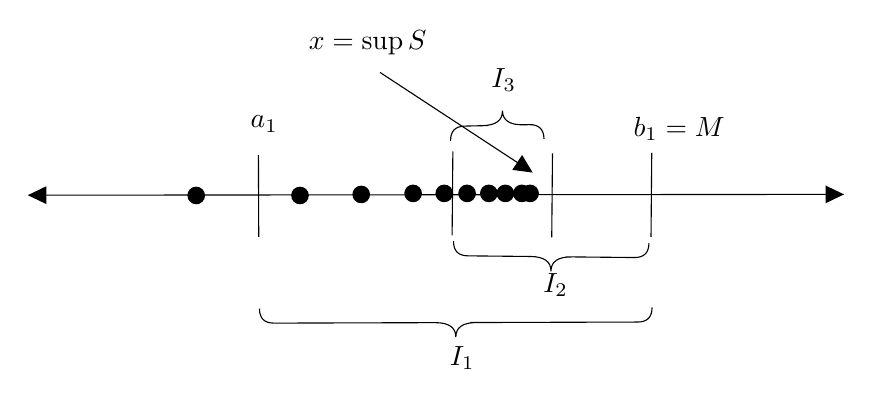
\begin{tikzpicture}[x=0.75pt,y=0.75pt,yscale=-1,xscale=1]
%uncomment if require: \path (0,196); %set diagram left start at 0, and has height of 196

%Straight Lines [id:da23809530369993093] 
\draw    (132.29,81.84) -- (519.56,81.45) ;
\draw [shift={(522.56,81.45)}, rotate = 179.94] [fill={rgb, 255:red, 0; green, 0; blue, 0 }  ][line width=0.08]  [draw opacity=0] (8.93,-4.29) -- (0,0) -- (8.93,4.29) -- cycle    ;
\draw [shift={(129.29,81.84)}, rotate = 359.94] [fill={rgb, 255:red, 0; green, 0; blue, 0 }  ][line width=0.08]  [draw opacity=0] (8.93,-4.29) -- (0,0) -- (8.93,4.29) -- cycle    ;
%Straight Lines [id:da9386714624284904] 
\draw    (429.91,61.5) -- (429.56,101.95) ;
%Shape: Circle [id:dp353816579177497] 
\draw  [fill={rgb, 255:red, 0; green, 0; blue, 0 }  ,fill opacity=1 ] (206.46,81.97) .. controls (206.46,79.78) and (208.24,78) .. (210.44,78) .. controls (212.63,78) and (214.41,79.78) .. (214.41,81.97) .. controls (214.41,84.17) and (212.63,85.95) .. (210.44,85.95) .. controls (208.24,85.95) and (206.46,84.17) .. (206.46,81.97) -- cycle ;
%Shape: Circle [id:dp09685381598729359] 
\draw  [fill={rgb, 255:red, 0; green, 0; blue, 0 }  ,fill opacity=1 ] (256.46,81.97) .. controls (256.46,79.78) and (258.24,78) .. (260.44,78) .. controls (262.63,78) and (264.41,79.78) .. (264.41,81.97) .. controls (264.41,84.17) and (262.63,85.95) .. (260.44,85.95) .. controls (258.24,85.95) and (256.46,84.17) .. (256.46,81.97) -- cycle ;
%Shape: Circle [id:dp21260541128458166] 
\draw  [fill={rgb, 255:red, 0; green, 0; blue, 0 }  ,fill opacity=1 ] (285.96,81.47) .. controls (285.96,79.28) and (287.74,77.5) .. (289.94,77.5) .. controls (292.13,77.5) and (293.91,79.28) .. (293.91,81.47) .. controls (293.91,83.67) and (292.13,85.45) .. (289.94,85.45) .. controls (287.74,85.45) and (285.96,83.67) .. (285.96,81.47) -- cycle ;
%Shape: Circle [id:dp3621837432113053] 
\draw  [fill={rgb, 255:red, 0; green, 0; blue, 0 }  ,fill opacity=1 ] (310.96,80.97) .. controls (310.96,78.78) and (312.74,77) .. (314.94,77) .. controls (317.13,77) and (318.91,78.78) .. (318.91,80.97) .. controls (318.91,83.17) and (317.13,84.95) .. (314.94,84.95) .. controls (312.74,84.95) and (310.96,83.17) .. (310.96,80.97) -- cycle ;
%Shape: Circle [id:dp107771568588785] 
\draw  [fill={rgb, 255:red, 0; green, 0; blue, 0 }  ,fill opacity=1 ] (325.96,80.97) .. controls (325.96,78.78) and (327.74,77) .. (329.94,77) .. controls (332.13,77) and (333.91,78.78) .. (333.91,80.97) .. controls (333.91,83.17) and (332.13,84.95) .. (329.94,84.95) .. controls (327.74,84.95) and (325.96,83.17) .. (325.96,80.97) -- cycle ;
%Shape: Circle [id:dp08646027047616078] 
\draw  [fill={rgb, 255:red, 0; green, 0; blue, 0 }  ,fill opacity=1 ] (336.96,80.97) .. controls (336.96,78.78) and (338.74,77) .. (340.94,77) .. controls (343.13,77) and (344.91,78.78) .. (344.91,80.97) .. controls (344.91,83.17) and (343.13,84.95) .. (340.94,84.95) .. controls (338.74,84.95) and (336.96,83.17) .. (336.96,80.97) -- cycle ;
%Shape: Circle [id:dp8250863396323576] 
\draw  [fill={rgb, 255:red, 0; green, 0; blue, 0 }  ,fill opacity=1 ] (347.46,80.97) .. controls (347.46,78.78) and (349.24,77) .. (351.44,77) .. controls (353.63,77) and (355.41,78.78) .. (355.41,80.97) .. controls (355.41,83.17) and (353.63,84.95) .. (351.44,84.95) .. controls (349.24,84.95) and (347.46,83.17) .. (347.46,80.97) -- cycle ;
%Shape: Circle [id:dp4391539941836895] 
\draw  [fill={rgb, 255:red, 0; green, 0; blue, 0 }  ,fill opacity=1 ] (355.41,80.97) .. controls (355.41,78.78) and (357.19,77) .. (359.38,77) .. controls (361.58,77) and (363.36,78.78) .. (363.36,80.97) .. controls (363.36,83.17) and (361.58,84.95) .. (359.38,84.95) .. controls (357.19,84.95) and (355.41,83.17) .. (355.41,80.97) -- cycle ;
%Shape: Circle [id:dp50430776286293] 
\draw  [fill={rgb, 255:red, 0; green, 0; blue, 0 }  ,fill opacity=1 ] (363.36,80.97) .. controls (363.36,78.78) and (365.13,77) .. (367.33,77) .. controls (369.52,77) and (371.3,78.78) .. (371.3,80.97) .. controls (371.3,83.17) and (369.52,84.95) .. (367.33,84.95) .. controls (365.13,84.95) and (363.36,83.17) .. (363.36,80.97) -- cycle ;
%Shape: Circle [id:dp47307652627528274] 
\draw  [fill={rgb, 255:red, 0; green, 0; blue, 0 }  ,fill opacity=1 ] (367.33,80.97) .. controls (367.33,78.78) and (369.11,77) .. (371.3,77) .. controls (373.5,77) and (375.27,78.78) .. (375.27,80.97) .. controls (375.27,83.17) and (373.5,84.95) .. (371.3,84.95) .. controls (369.11,84.95) and (367.33,83.17) .. (367.33,80.97) -- cycle ;
%Straight Lines [id:da4627187915413793] 
\draw    (299,22.7) -- (370.05,69.3) ;
\draw [shift={(372.56,70.95)}, rotate = 213.26] [fill={rgb, 255:red, 0; green, 0; blue, 0 }  ][line width=0.08]  [draw opacity=0] (8.93,-4.29) -- (0,0) -- (8.93,4.29) -- cycle    ;
%Straight Lines [id:da6983959365845951] 
\draw    (240.41,62.5) -- (240.56,101.95) ;
%Straight Lines [id:da19549870057926433] 
\draw    (334.09,60.75) -- (333.73,101.2) ;
%Shape: Brace [id:dp38843570822590734] 
\draw   (240.91,136.5) .. controls (240.92,141.17) and (243.26,143.49) .. (247.93,143.48) -- (325.5,143.25) .. controls (332.17,143.23) and (335.51,145.55) .. (335.52,150.22) .. controls (335.51,145.55) and (338.83,143.21) .. (345.5,143.19)(342.5,143.2) -- (423.08,142.96) .. controls (427.75,142.95) and (430.07,140.61) .. (430.06,135.94) ;
%Shape: Brace [id:dp7338518996860539] 
\draw   (334.41,104) .. controls (334.36,108.67) and (336.67,111.02) .. (341.34,111.07) -- (371.41,111.37) .. controls (378.08,111.44) and (381.39,113.81) .. (381.34,118.48) .. controls (381.39,113.81) and (384.74,111.51) .. (391.41,111.58)(388.41,111.55) -- (421.49,111.88) .. controls (426.16,111.93) and (428.51,109.62) .. (428.56,104.95) ;
%Straight Lines [id:da9284476288664791] 
\draw    (382.09,61.75) -- (381.73,102.2) ;
%Shape: Brace [id:dp9578258559471491] 
\draw   (378,54.7) .. controls (377.89,50.03) and (375.51,47.75) .. (370.85,47.86) -- (368.12,47.92) .. controls (361.46,48.07) and (358.08,45.81) .. (357.97,41.14) .. controls (358.08,45.81) and (354.8,48.21) .. (348.13,48.36)(351.13,48.3) -- (339.84,48.55) .. controls (335.17,48.65) and (332.89,51.03) .. (333,55.7) ;

% Text Node
\draw (419.91,42.9) node [anchor=north west][inner sep=0.75pt]    {$b_{1} =M$};
% Text Node
\draw (263.41,1.4) node [anchor=north west][inner sep=0.75pt]    {$x=\sup S$};
% Text Node
\draw (235.41,42.4) node [anchor=north west][inner sep=0.75pt]    {$a_{1}$};
% Text Node
\draw (331.41,153.4) node [anchor=north west][inner sep=0.75pt]    {$I_{1}$};
% Text Node
\draw (376.41,118.4) node [anchor=north west][inner sep=0.75pt]    {$I_{2}$};
% Text Node
\draw (351.41,19.4) node [anchor=north west][inner sep=0.75pt]    {$I_{3}$};


\end{tikzpicture}



If $\displaystyle S$ is a finite subset of $\displaystyle \mathbf{R}$, then $\displaystyle \sup S=\max\{x:x\in S\}$. 



Let's assume that $\displaystyle S$ is an infinite set. Let $\displaystyle I_{1} =[ a_{1} ,b_{1}]$ be a closed interval such that $\displaystyle b_{1} =M$, $\displaystyle a_{1} < b_{1}$ with $\displaystyle [ a_{1} ,b_{1}]$ containing an infinite number of terms of $\displaystyle S$. We bisect $\displaystyle I_{1}$ into two intervals $\displaystyle L_{1} =[ a_{1} ,( a_{1} +b_{1}) /2]$ and $\displaystyle R_{1} =[( a_{1} +b_{1}) /2,b_{1}]$. 



We define $\displaystyle I_{2} =L_{1}$ if $\displaystyle R_{1} \cap S=\emptyset $ else $\displaystyle I_{2} =R_{1}$. In general,


\begin{equation*}
I_{k+1} =\begin{cases}
L_{k} & \text{if } R_{k} \cap S=\emptyset \\
R_{k} & \text{otherwise}
\end{cases}
\end{equation*}
Since 


\begin{equation*}
I_{1} \supseteq I_{2} \supseteq I_{3} \supseteq \dotsc \supseteq I_{k} \supseteq I_{k+1} \supseteq \dotsc 
\end{equation*}
by the Nested Interval Property (NIP) there exists an element $\displaystyle s\in \bigcap _{k=1}^{\infty } I_{k}$. \ 



Our claim is that $\displaystyle s=\sup S$. Since $\displaystyle ( 1/2)^{n}\rightarrow 0$, for all $\displaystyle \epsilon  >0$, there exists $\displaystyle N$ such that for all $\displaystyle n >N$, $\displaystyle l( I_{n}) =\frac{l( I_{1})}{2^{n}} < \epsilon $. Thus, $\displaystyle \lim a_{n} =\lim b_{n} =s$. 



(1) $\displaystyle s$ is an upper bound for $\displaystyle S$. 



It is clear that all $\displaystyle b_{n}$'s are an upper bound $\displaystyle S$. By the Order Limit Theorem, $\displaystyle x\leq s$ for all $\displaystyle x\in S$.



(2) $\displaystyle I_{k} \cap S\neq \emptyset $ for all $\displaystyle k\in \mathbf{N}$. Thus, for all $\displaystyle \epsilon  >0$, $\displaystyle \exists x\in I_{k} \cap S$ such that $\displaystyle s-\epsilon < x$. Consequently, by lemma 1.3.8, $\displaystyle s=\sup S$.



\textbf{Abbott 2.5.5}. Assume that $\displaystyle ( a_{n})$ is a bounded sequence with the property that every convergent subsequence of $\displaystyle ( a_{n})$ converges to the same limit $\displaystyle a\in \mathbf{R}$. Show that $\displaystyle ( a_{n})$ must converge to $\displaystyle a$.



\textbf{Proof}.



We are given that $\displaystyle ( a_{n})$ is a bounded sequence with the property that every convergent subsequence $\displaystyle ( a_{n})$ converges to the same limit $\displaystyle a\in \mathbf{R}$. We proceed by contradiction. 

Assume that $\displaystyle ( a_{n})$ is a divergent sequence.



From 2.5.2 (c), since $\displaystyle ( a_{n})$ is a bounded and divergent sequence, there exist atleast two subsequences of $\displaystyle ( a_{n})$ that converge to different limits. This contradicts the fact that every convergent subsequence of $\displaystyle ( a_{n})$ converges to the same limit $\displaystyle a\in \mathbf{R}$. 



Hence, our initial assumption is false. $\displaystyle ( a_{n})$ must be a convergent sequence.



\textbf{Abbott 2.5.6}. Use a similar strategy to the one in example 2.5.3. to show that $\displaystyle b^{1/n}$ exists for all $\displaystyle b\geq 0\ $and find the value of the limit.



\textbf{Solution}.

Assume that $\displaystyle 0\leq b< 1$. Then, since 


\begin{equation*}
b\leq b^{1/2} \leq b^{1/3} \leq b^{1/4} \leq \dotsc 
\end{equation*}
$\displaystyle ( b_{n})$ is a monotonically increasing sequence and bounded by $\displaystyle 1$, $\displaystyle ( b_{n})$ is a convergent sequence. Let $\displaystyle \lim b_{n} =l$. Since, $\displaystyle \lim b_{2n} =\lim \left( b^{1/n}\right)^{1/2} =\sqrt{l}$, we have that $\displaystyle \sqrt{l} =l$. So, $\displaystyle l=1$.



Assume that $\displaystyle b\geq 1$. Then, since


\begin{equation*}
b\geq b^{1/2} \geq b^{1/3} \geq b^{1/4} \geq \dotsc 
\end{equation*}
$\displaystyle \left( b^{1/n}\right)$ is a monotonically decreasing sequence bounded below by $\displaystyle 1$. Again, $\displaystyle \left( b^{1/n}\right)\rightarrow 1$.



\textbf{Abbott 2.5.7}. Extend the result proved in example 2.5.3 to the case $\displaystyle |b|< 1$, that is show that $\displaystyle \lim b^{n} =0$ if and only if $\displaystyle -1< b< 1$.



\textbf{Proof}.

($\displaystyle \Longrightarrow $) direction.

Assume that $\displaystyle \lim b^{n} =0$. Then, $\displaystyle \lim |b^{n} |=0$. We proceed by contradiction. Assume that $\displaystyle |b|\geq 1$. Then:


\begin{equation*}
1\leq |b|\leq |b|^{2} \leq |b|^{3} \leq \dotsc \leq |b|^{n} \leq \dotsc 
\end{equation*}


Since $\displaystyle \left( |b|^{n}\right)$ is convergent, by the Order Limit Theorem:


\begin{equation*}
1\leq \lim |b|^{n}
\end{equation*}


This contradicts the fact that $\displaystyle \lim |b|^{n} =0$.



($\displaystyle \Longleftarrow $) direction.



Assume that $\displaystyle -1< b< 0$. Pick an arbitrary $\displaystyle \epsilon  >0$. We pick $\displaystyle N\in \mathbf{N}$ such that,


\begin{equation*}
|b|^{N} < \epsilon 
\end{equation*}
 \ that is :


\begin{equation*}
\begin{array}{ r l }
N\log |b| & < \epsilon \\
\therefore N &  >\frac{\epsilon }{\log |b|}
\end{array}
\end{equation*}
Then, for all $\displaystyle n >N$, we have:


\begin{equation*}
b^{n} \in ( -\epsilon ,\epsilon )
\end{equation*}
Consequently, $\displaystyle \lim b^{n} =0$. 



If $\displaystyle b=0$, then the constant sequence $\displaystyle ( 0,0,0,\dotsc )$ converges to $\displaystyle 0$.



\textbf{Abbott 2.6.1}. Suppy a proof for the Theorem 2.6.2.



Every convergent sequence is a Cauchy sequence.



\textbf{Proof.}

Let $\displaystyle ( x_{n})$ be a convergent sequence. Assume that $\displaystyle ( x_{n})\rightarrow x$. Pick an arbitrary $\displaystyle \epsilon  >0$. There exists $\displaystyle N\in \mathbf{N}$, for all $\displaystyle n\geq N$, the distance


\begin{equation*}
|x_{n} -x|< \epsilon /2
\end{equation*}


Now, consider the expression $\displaystyle |x_{n} -x_{m} |$ where $\displaystyle m,n\geq N$. We have:


\begin{equation*}
\begin{array}{ c l c }
|x_{n} -x_{m} | & =|( x_{n} -x) -( x_{m} -x) | & \\
 & \leq |x_{n} -x|+|x_{m} -x| & \left\{\text{Triangle Inequality}\right\}\\
 & < \frac{\epsilon }{2} +\frac{\epsilon }{2} =\epsilon  & 
\end{array}
\end{equation*}
Thus, $\displaystyle ( x_{n})$ is a Cauchy sequence.



\textbf{Abbott 2.6.2}. Give an example of each of the following or argue that such a request is impossible.



(a) A Cauchy sequence that is not monotone.



\textbf{Proof}.

Consider $\displaystyle a_{n} =\frac{( -1)^{n}}{n}$. This is a convergent sequence and hence Cauchy. Moreover, it is not monotone.



(b) A Cauchy sequence with an unbounded subsequence. 

\textbf{Solution}.



This request is impossible. By Lemma 2.6.3, Cauchy sequences are bounded. Thus, there exists $\displaystyle M >0$, for all $\displaystyle n\in \mathbf{N}$, such that $\displaystyle |x_{n} |\leq M$. Let $\displaystyle ( x_{n_{k}})$ be any arbitrary subsequence of $\displaystyle ( x_{n})$. Then it follows that, $\displaystyle |x_{n_{k}} |\leq M$ for all $\displaystyle k\in \mathbf{N}$.



Thus, all subsequences of a Cauchy sequence are bounded.



(c) A divergent montone sequence with a Cauchy subsequence.



\textbf{Solution}.



This request is impossible. A divergent monotone sequence cannot contain a Cauchy subsequence. We proceed by contradiction.



Let $\displaystyle ( x_{n})$ be a divergent monotone sequence. Assume that, there exists \ a Cauchy subsequence $\displaystyle ( x_{n_{k}})$ of $\displaystyle ( x_{n})$. 



We know, from theorem 2.6.4, that if a sequence is convergent $\displaystyle \Longleftrightarrow $the sequence is Cauchy. So, Cauchy sequences are convergent. Thus, if a sequence is divergent, it is not Cauchy. Thus, $\displaystyle ( x_{n})$ is not Cauchy.



Carefully negating the definition of a Cauchy sequence, we have that $\displaystyle \exists \epsilon _{0}  >0$, for all $\displaystyle N\in \mathbf{N}$, such that for some $\displaystyle n >m\geq N$, it follows that $\displaystyle |x_{n} -x_{m} |\geq \epsilon _{0}$. 



We know that $\displaystyle ( x_{n_{k}})$ is Cauchy. Pick $\displaystyle \epsilon =\epsilon _{0}$. There exists $\displaystyle C\in \mathbf{N}$, such that for all $\displaystyle n_{k+1}  >n_{k} \geq C$, it follows that $\displaystyle |x_{n_{k+1}} -x_{n_{k}} |< \epsilon _{0}$. 



Since $\displaystyle ( x_{n})$ is monotone, it follows that all the intermediate terms $\displaystyle \{x_{n} :n\in \mathbf{N} ,n_{k} < n< n_{k+1}\}$ lie between $\displaystyle x_{n_{k}}$ and $\displaystyle x_{n_{k+1}}$ on the real line. Consequently, the distance amongst them must be smaller than $\displaystyle \epsilon _{0}$. Thus, we conclude that, for all $\displaystyle n >m\geq C$, $\displaystyle |x_{n} -x_{m} |< \epsilon _{0}$. 



This is a contradiction. Our initial assumption is false.



(d) An unbounded sequence containing a subsequence that is Cauchy.



Consider the sequence formed by juxtaposing the terms of the sequence $\displaystyle ( a_{n}) =( 0,0,0,0,\dotsc )$ which is Cauchy and $\displaystyle ( b_{n}) =( 1,2,3,4,5,\dotsc )$ which is unbounded. The shuffle sequence $\displaystyle ( c_{n}) =( 0,1,0,2,0,3,\dotsc )$ is unbounded and contains a Cauchy subsequence.



\textbf{Abbott 2.6.3}. If $\displaystyle ( x_{n})$ and $\displaystyle ( y_{n})$ are Cauchy sequences, then one easy way to prove that $\displaystyle ( x_{n} +y_{n})$ is Cauchy is to use the Cauchy criterion. By theorem 2.6.4, $\displaystyle ( x_{n})$ and $\displaystyle ( y_{n})$ must be convergent, and the Algebraic Limit Theorem the implies that $\displaystyle ( x_{n} +y_{n})$ is convergent and hence Cauchy.



(a) Give a direct argument that $\displaystyle ( x_{n} +y_{n})$ is a Cauchy sequence that does not use the Cauchy criterion or the Algebraic Limit Theorem. 



\textbf{Proof}.



Pick an arbitrary $\displaystyle \epsilon  >0$. 



Since $\displaystyle ( x_{n})$ is a Cauchy sequence, there exists $\displaystyle N_{1}  >0$, such that for all $\displaystyle n >m\geq N_{1}$, we have $\displaystyle |x_{n} -x_{m} |< \epsilon /2$.



Since $\displaystyle ( y_{n})$ is a Cauchy sequence, there exists $\displaystyle N_{2}  >0$, such that for all $\displaystyle n >m\geq N_{2}$, we have $\displaystyle |y_{n} -y_{m} |< \epsilon /2$.



Consider two arbitrary terms $\displaystyle z_{m} ,z_{n}$ of the sum sequence $\displaystyle ( z_{n}) =( x_{n} +y_{n})$, such that $\displaystyle m,n\geq N=\max\{N_{1} ,N_{2}\}$. We have:




\begin{equation*}
\begin{array}{ c l c }
|z_{n} -z_{m} | & =|x_{n} +y_{n} -( x_{m} +y_{m}) | & \\
 & \leq |x_{n} -x_{m} |+|y_{n} -y_{m} | & \left\{\text{Triangle Inequality}\right\}\\
 & < \frac{\epsilon }{2} +\frac{\epsilon }{2} =\epsilon  & 
\end{array}
\end{equation*}
Thus, by definition, $\displaystyle ( z_{n})$ is a Cauchy sequence.



(b) Do the same for the product $\displaystyle ( x_{n} y_{n})$.



\textbf{Proof}.



Pick an arbitrary $\displaystyle \epsilon  >0$. 



Consider two arbitrary terms $\displaystyle z_{m} ,z_{n}$ of the product sequence $\displaystyle ( z_{n}) =( x_{n} y_{n})$. We have:




\begin{equation*}
\begin{array}{ c l c }
|z_{n} -z_{m} | & =|x_{n} y_{n} -x_{m} y_{m} | & \\
 & =|x_{n} y_{n} -x_{m} y_{n} +x_{m} y_{n} -x_{m} y_{m} | & \\
 & \leq |x_{n} y_{n} -x_{m} y_{n} |+|x_{m} y_{n} -x_{m} y_{m} | & \left\{\text{Triangle Inequality}\right\}\\
 & =|y_{n} ||x_{n} -x_{m} |+|x_{m} ||y_{n} -y_{m} | & 
\end{array}
\end{equation*}
Since $\displaystyle ( x_{n})$ and $\displaystyle ( y_{n})$ are Cauchy sequences and Cauchy sequences are bounded, it follows that $\displaystyle ( x_{n})$ and $\displaystyle ( y_{n})$ are bounded. There exists $\displaystyle M_{1}  >0$, for all $\displaystyle n\in \mathbf{N}$, such that $\displaystyle |x_{n} |\leq M_{1}$. There exists $\displaystyle M_{2}  >0$, for all $\displaystyle n\in \mathbf{N}$, such that $\displaystyle |y_{n} |\leq M_{2}$. 



Since $\displaystyle ( x_{n})$ is a Cauchy sequence, there exists $\displaystyle N_{1}  >0$, such that for all $\displaystyle n >m\geq N_{1}$, we have $\displaystyle |x_{n} -x_{m} |< \epsilon /2M_{2}$.



Since $\displaystyle ( y_{n})$ is a Cauchy sequence, there exists $\displaystyle N_{2}  >0$, such that for all $\displaystyle n >m\geq N_{2}$, we have $\displaystyle |y_{n} -y_{m} |< \epsilon /2M_{1}$. \ 



Thus, for all $\displaystyle n >m\geq N=\max\{N_{1} ,N_{2}\}$, we can write:




\begin{equation*}
\begin{array}{ c l }
|z_{n} -z_{m} | & \leq |y_{n} ||x_{n} -x_{m} |+|x_{m} ||y_{n} -y_{m} |\\
 & < M_{2} \cdot \frac{\epsilon }{2M_{2}} +M_{1} \cdot \frac{\epsilon }{2M_{1}} =\epsilon 
\end{array}
\end{equation*}
Consequently, $\displaystyle ( z_{n})$ is Cauchy.



\textbf{Abbott 2.6.4}. Let $\displaystyle ( a_{n})$ and $\displaystyle ( b_{n})$ be Cauchy sequences. Decide whether each of the following sequences is a Cauchy sequence justifying each conclusion.



(a) $\displaystyle c_{n} =|a_{n} -b_{n} |$.



\textbf{Proof}.



If $\displaystyle ( a_{n})$ and $\displaystyle ( b_{n})$ are Cauchy sequences, by the Cauchy criterion, $\displaystyle ( a_{n})$ and $\displaystyle ( b_{n})$ are convergent. Applying the algebraic limit theorem, $\displaystyle ( a_{n} -b_{n})$ is a convergent sequence. Moreover, if $\displaystyle ( x_{n})$ is a convergent sequence, then from Exercise 2.3.10, $\displaystyle |x_{n} |$ is a convergent sequence. Thus, $\displaystyle |a_{n} -b_{n} |$ is a convergent sequence, and there Cauchy.



(b) $\displaystyle c_{n} =( -1)^{n} a_{n}$.



This conclusion is false. Consider the counterexample:



$\displaystyle c_{n} =( -1)^{n}\left( 1+\frac{1}{n}\right)$ where $\displaystyle a_{n} =1+\frac{1}{n}$. $\displaystyle ( a_{n})$ is Cauchy, but $\displaystyle ( c_{n})$ is not a Cauchy sequence.



(c) $\displaystyle c_{n} =[[ a_{n}]]$ where $\displaystyle [[ x]]$ is the greatest integer less than or equal to $\displaystyle x$.



\textbf{Proof}.



This proposition is false. Consider the sequence $\displaystyle a_{n} =\frac{( -1)^{n}}{n}$. 




\begin{equation*}
( a_{n}) =\left( -1,\frac{1}{2} ,-\frac{1}{3} ,\frac{1}{4} ,-\frac{1}{5} ,\dotsc \right)
\end{equation*}
so $\displaystyle ( a_{n})\rightarrow 0$ whilst 


\begin{equation*}
( c_{n}) =( -1,0,-1,0,-1,0,\dotsc )
\end{equation*}
so $\displaystyle ( c_{n})$ is not a Cauchy sequence.



\textbf{Abbott 2.6.5}. Consider the following (invented) definition: A sequence $\displaystyle ( s_{n})$ is pseudo-Cauchy if for all $\displaystyle \epsilon  >0$, there exists an $\displaystyle N$ such that if $\displaystyle n\geq N$, then $\displaystyle |s_{n+1} -s_{n} |< \epsilon $. 



Decide for which one of the following two propositions is actually true. Supply a proof for the valid statement and a counterexample for the other.



(i) Pseudo-Cauchy sequences are bounded.



\textbf{Solution}.



This proposition is false.

Consider the sequence of partial sums $\displaystyle s_{n} =\sum _{k=1}^{n}\frac{1}{n}$. This is a pseudo-cauchy sequence. The difference between successive terms can be made as small as possible. However, the sum keeps increasing ever-so slowly, and does not stop even if you took one million, one billion or one trillion terms.

image[mc://users/ec70f086d36050429d70122065f9a453/contents/cd362e2d1daba4cb43f2ec8530e0dcae-1oDju9eE1t-harmonic_series.png]



(ii) If $\displaystyle ( x_{n})$ and $\displaystyle ( y_{n})$ are pseudo-Cauchy, then $\displaystyle ( x_{n} +y_{n})$ is Pseudo-Cauchy as well.



This proposition is true.



Pick an arbitrary $\displaystyle \epsilon  >0$.



Since $\displaystyle ( x_{n})$ is pseudo-cauchy, $\displaystyle \exists N_{1}$ such that for all $\displaystyle n\geq N_{1}$, we have:


\begin{equation*}
|x_{n+1} -x_{n} |< \epsilon /2
\end{equation*}


Since $\displaystyle ( y_{n})$ is pseudo-cauchy, $\displaystyle \exists N_{2}$ such that for all $\displaystyle n\geq N_{2}$, we have:


\begin{equation*}
|y_{n+1} -y_{n} |< \epsilon /2
\end{equation*}
Let $\displaystyle N=\max\{N_{1} ,N_{2}\}$.



Then, for all $\displaystyle n\geq N$, we have:


\begin{equation*}
\begin{array}{ c l c }
|( x_{n+1} +y_{n+1}) -( x_{n} +y_{n}) | & =| ( x_{n+1} -x_{n}) +( y_{n+1} -y_{n})|  & \\
 & \leq | ( x_{n+1} -x_{n}) |\ +|( y_{n+1} -y_{n}) | & \left\{\text{Triangle Inequality}\right\}\\
 & < \frac{\epsilon }{2} +\frac{\epsilon }{2} =\epsilon  & 
\end{array}
\end{equation*}
Thus, $\displaystyle ( x_{n} +y_{n})$ is pseudo-Cauchy.



\textbf{Abbott 2.7.1}. Proving the Alternating Series Test (Theorem 2.7.7) amounts to show that the sequence of partial sums 


\begin{equation*}
s_{n} =a_{1} -a_{2} +a_{3} -\dotsc \pm a_{n}
\end{equation*}
converges. Different characterizations of completeness lead to different proofs.



(a) Prove the Alternating Series Test by showing that $\displaystyle ( s_{n})$ is a Cauchy sequence.



\textbf{Proof}.



Firstly, we have $\displaystyle a_{1} \geq a_{n}$ for all $\displaystyle n\geq 1$. Taking limits on both sides, by the Order Limit theorem, $\displaystyle a_{1} \geq \lim a_{n} =0$. Similarly, we can conclude 



(a) Consider the distance $\displaystyle |s_{n} -s_{m} |$. We are interested to make this distance as small as we please.




\begin{equation*}
\begin{array}{ c l }
|s_{n} -s_{m} | & =|( -1)^{m} a_{m+1} +\dotsc +( -1)^{n} a_{n} |\\
 & 
\end{array}
\end{equation*}
(b) Consider the sequence of partial sums $\displaystyle ( s_{1} ,s_{2} ,s_{3} ,s_{4} ,\dotsc )$



Let $\displaystyle S=\{s_{1} ,s_{2} ,s_{3} ,\dotsc \}$.




\tikzset{every picture/.style={line width=0.75pt}} %set default line width to 0.75pt        

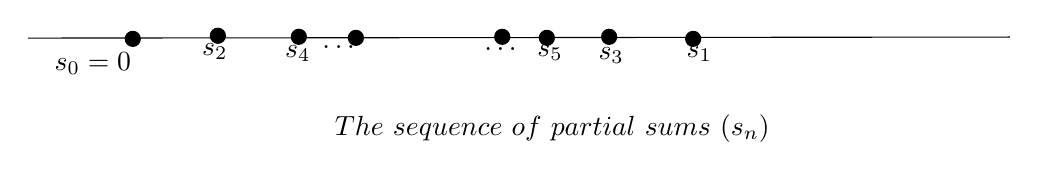
\begin{tikzpicture}[x=0.75pt,y=0.75pt,yscale=-1,xscale=1]
%uncomment if require: \path (0,154); %set diagram left start at 0, and has height of 154

%Straight Lines [id:da36241535270228753] 
\draw    (30.5,70.75) -- (503.5,70.25) ;
%Shape: Circle [id:dp541915650910596] 
\draw  [fill={rgb, 255:red, 0; green, 0; blue, 0 }  ,fill opacity=1 ] (77.25,71.13) .. controls (77.25,69.12) and (78.87,67.5) .. (80.88,67.5) .. controls (82.88,67.5) and (84.5,69.12) .. (84.5,71.13) .. controls (84.5,73.13) and (82.88,74.75) .. (80.88,74.75) .. controls (78.87,74.75) and (77.25,73.13) .. (77.25,71.13) -- cycle ;
%Shape: Circle [id:dp7237740080828454] 
\draw  [fill={rgb, 255:red, 0; green, 0; blue, 0 }  ,fill opacity=1 ] (347.25,71.13) .. controls (347.25,69.12) and (348.87,67.5) .. (350.88,67.5) .. controls (352.88,67.5) and (354.5,69.12) .. (354.5,71.13) .. controls (354.5,73.13) and (352.88,74.75) .. (350.88,74.75) .. controls (348.87,74.75) and (347.25,73.13) .. (347.25,71.13) -- cycle ;
%Shape: Circle [id:dp5509092505012745] 
\draw  [fill={rgb, 255:red, 0; green, 0; blue, 0 }  ,fill opacity=1 ] (118.25,69.63) .. controls (118.25,67.62) and (119.87,66) .. (121.88,66) .. controls (123.88,66) and (125.5,67.62) .. (125.5,69.63) .. controls (125.5,71.63) and (123.88,73.25) .. (121.88,73.25) .. controls (119.87,73.25) and (118.25,71.63) .. (118.25,69.63) -- cycle ;
%Shape: Circle [id:dp32465057417986576] 
\draw  [fill={rgb, 255:red, 0; green, 0; blue, 0 }  ,fill opacity=1 ] (306.75,70.13) .. controls (306.75,68.12) and (308.37,66.5) .. (310.38,66.5) .. controls (312.38,66.5) and (314,68.12) .. (314,70.13) .. controls (314,72.13) and (312.38,73.75) .. (310.38,73.75) .. controls (308.37,73.75) and (306.75,72.13) .. (306.75,70.13) -- cycle ;
%Shape: Circle [id:dp542752663091207] 
\draw  [fill={rgb, 255:red, 0; green, 0; blue, 0 }  ,fill opacity=1 ] (157.25,70.13) .. controls (157.25,68.12) and (158.87,66.5) .. (160.88,66.5) .. controls (162.88,66.5) and (164.5,68.12) .. (164.5,70.13) .. controls (164.5,72.13) and (162.88,73.75) .. (160.88,73.75) .. controls (158.87,73.75) and (157.25,72.13) .. (157.25,70.13) -- cycle ;
%Shape: Circle [id:dp224525675453076] 
\draw  [fill={rgb, 255:red, 0; green, 0; blue, 0 }  ,fill opacity=1 ] (276.75,70.63) .. controls (276.75,68.62) and (278.37,67) .. (280.38,67) .. controls (282.38,67) and (284,68.62) .. (284,70.63) .. controls (284,72.63) and (282.38,74.25) .. (280.38,74.25) .. controls (278.37,74.25) and (276.75,72.63) .. (276.75,70.63) -- cycle ;
%Shape: Circle [id:dp010209523647260355] 
\draw  [fill={rgb, 255:red, 0; green, 0; blue, 0 }  ,fill opacity=1 ] (184.75,70.63) .. controls (184.75,68.62) and (186.37,67) .. (188.38,67) .. controls (190.38,67) and (192,68.62) .. (192,70.63) .. controls (192,72.63) and (190.38,74.25) .. (188.38,74.25) .. controls (186.37,74.25) and (184.75,72.63) .. (184.75,70.63) -- cycle ;
%Shape: Circle [id:dp6888323480686172] 
\draw  [fill={rgb, 255:red, 0; green, 0; blue, 0 }  ,fill opacity=1 ] (255.25,70.13) .. controls (255.25,68.12) and (256.87,66.5) .. (258.88,66.5) .. controls (260.88,66.5) and (262.5,68.12) .. (262.5,70.13) .. controls (262.5,72.13) and (260.88,73.75) .. (258.88,73.75) .. controls (256.87,73.75) and (255.25,72.13) .. (255.25,70.13) -- cycle ;

% Text Node
\draw (42,76.4) node [anchor=north west][inner sep=0.75pt]    {$s_{0} =0$};
% Text Node
\draw (346.5,72.9) node [anchor=north west][inner sep=0.75pt]    {$s_{1}$};
% Text Node
\draw (113,71.9) node [anchor=north west][inner sep=0.75pt]    {$s_{2}$};
% Text Node
\draw (304,73.9) node [anchor=north west][inner sep=0.75pt]    {$s_{3}$};
% Text Node
\draw (153,72.9) node [anchor=north west][inner sep=0.75pt]    {$s_{4}$};
% Text Node
\draw (274.5,72.4) node [anchor=north west][inner sep=0.75pt]    {$s_{5}$};
% Text Node
\draw (171,72.9) node [anchor=north west][inner sep=0.75pt]    {$\dotsc $};
% Text Node
\draw (249,73.9) node [anchor=north west][inner sep=0.75pt]    {$\dotsc $};
% Text Node
\draw (177,106.4) node [anchor=north west][inner sep=0.75pt]    {$The\ sequence\ of\ partial\ sums\ ( s_{n})$};


\end{tikzpicture}



Define $\displaystyle I_{1} =[ 0,s_{1}]$. We bisect the interval $\displaystyle I_{1}$ into two halves $\displaystyle L_{1}$ and $\displaystyle R_{1}$. We let:


\begin{equation*}
I_{2} =\begin{cases}
R_{1} & \text{if } R_{1} \cap S\ \text{contains an infinite number of points}\\
L_{1} & \text{otherwise}
\end{cases}
\end{equation*}
 

In general, we let:


\begin{equation*}
I_{k+1} =\begin{cases}
R_{k} & \text{if } R_{k} \cap S\ \text{contains an infinite number of points of } S\\
L_{k} & \text{otherwise}
\end{cases}
\end{equation*}
We have $\displaystyle I_{k} \supseteq I_{k+1}$. By the Nested Interval Property, there exists $\displaystyle s\in \bigcap _{k=1}^{\infty } I_{k}$. Our claim is that $\displaystyle ( s_{n})\rightarrow s$. Pick an arbitrary $\displaystyle \epsilon  >0$. 



We can pick $\displaystyle K$ such that:


\begin{equation*}
l( I_{K}) =\frac{s_{1}}{2^{K-1}} < \epsilon 
\end{equation*}
Then, for all $\displaystyle k >K$, since $\displaystyle s \in I_{k}$, we must have that $\displaystyle |s_{k} -s|< \epsilon $. Thus, $\displaystyle ( s_{k})\rightarrow s$.



(c) We find that:


\begin{equation*}
\begin{array}{ c l c }
s_{2k+2} & =s_{2k} +( a_{2k+1} -a_{2k+2}) & \\
 & \geq s_{2k} & \left\{\text{since} \ ( a_{2k+1} -a_{2k+2}) \geq 0\right\}
\end{array}
\end{equation*}
And,
\begin{equation*}
\begin{array}{ c l c }
s_{2k+3} & =s_{2k+1} -a_{2k+2} +a_{2k+3} & \\
 & =s_{2k+1} -( a_{2k+2} -a_{2k+3}) & \\
 & \leq s_{2k+1} & \left\{\text{since} \ ( a_{2k+2} -a_{2k+3}) \geq 0\right\}
\end{array}
\end{equation*}
Thus, the subsequence $\displaystyle ( s_{2n})$ is a monotonically increasing sequence. And $\displaystyle ( s_{2n+1})$ is a monotonically decreasing sequence. Moreover,
\begin{equation*}
\begin{array}{ c l }
s_{2n} & =s_{2n+1} -a_{2n+1}\\
 & \leq s_{2n+1}
\end{array}
\end{equation*}
And therefore we conclude:


\begin{equation*}
0\leq s_{2} \leq s_{4} \leq s_{6} \leq \dotsc \leq s_{2n} \leq s_{2n+1} \leq \dotsc \leq s_{5} \leq s_{3} \leq s_{1}
\end{equation*}


Since $\displaystyle ( s_{2n})$ is monotonically increasing and bounded above by all $\displaystyle ( s_{2n+1})$'s, by the Monotone Convergence Theorem (MCT), $\displaystyle ( s_{2n})$ is a convergent sequence. 



Since $\displaystyle ( s_{2n+1})$ is monotonically increasing and bounded below by all $\displaystyle ( s_{2n})$'s, by the Monotone Convergence Theorem (MCT), $\displaystyle ( s_{2n+1})$ is a convergent sequence. 



The limits of $\displaystyle ( s_{2n})$ and $\displaystyle ( s_{2n+1})$ could be different. We will prove that the limits are same.



Let $\displaystyle s=\lim s_{2n}$. Pick an arbitrary $\displaystyle \epsilon  >0$. Consider the $\displaystyle \epsilon -$neighbourhood $\displaystyle ( s-\epsilon ,s+\epsilon )$. 



There exists $\displaystyle N_{1} \in \mathbf{N}$, such that for all $\displaystyle n\geq N_{1}$, $\displaystyle s_{2n} \in ( s-\epsilon ,s+\epsilon )$. 



There exists $\displaystyle N_{2} \in \mathbf{N}$, such that for all $\displaystyle n\geq N_{2}$, $\displaystyle |a_{2n+1} |< \epsilon /2$



 Let $\displaystyle N=\max\{N_{1} ,N_{2}\}$. Then, $\displaystyle 2N+1\ \geq 2N_{1} +1 >2N_{1}$ and $\displaystyle 2N+1\geq 2N_{2} +1$. Consider the distance:
\begin{equation*}
\begin{array}{ c l }
|s_{2N+1} -s| & =|s_{2N+1} -s_{2N} +s_{2N} -s|\\
 & \leq |s_{2N+1} -s_{2N} |+|s_{2N} -s|\\
 & =|a_{2N+1} |+|s_{2N} -s|\\
 & < \frac{\epsilon }{2} +\frac{\epsilon }{2} =\epsilon 
\end{array}
\end{equation*}


So, $\displaystyle s_{2N}$ and $\displaystyle s_{2N+1}$ belong to $\displaystyle ( s-\epsilon ,s+\epsilon )$. Since, 


\begin{equation*}
s-\epsilon < s_{2N} \leq s_{2N+2} \leq \dotsc \leq s_{2N+3} \leq s_{2N+1} < s+\epsilon 
\end{equation*}


we have that for all $\displaystyle n\geq N$, $\displaystyle s_{n} \in ( s-\epsilon ,s+\epsilon )$. Consequently, $\displaystyle ( s_{n})\rightarrow s$.



\textbf{Abbott 2.7.2}. Decide whether each of the following series converges or diverges:



(a) $\displaystyle \sum _{n=1}^{\infty }\frac{1}{2^{n} +n}$



We have: 
\begin{equation*}
0\leq \frac{1}{2^{n} +n} \leq \frac{1}{2^{n}}
\end{equation*}
Since the infinite series$\displaystyle \sum _{n=1}^{\infty }\frac{1}{2^{n}}$ converges, by the comparision test, $\displaystyle \sum _{n=1}^{\infty }\frac{1}{2^{n} +n}$ also converges.



(b) $\displaystyle \sum _{n=1}^{\infty }\frac{\sin( n)}{n^{2}}$.



We have:


\begin{equation*}
0\leq \frac{|\sin n|}{n^{2}} \leq \frac{1}{n^{2}}
\end{equation*}
Since $\displaystyle \sum _{n=1}^{\infty }\frac{1}{n^{p}}$ converges if $\displaystyle p >1$, by the comparision test, $\displaystyle \sum _{n=1}^{\infty }\frac{|\sin n|}{n^{2}}$ converges. By the absolute convergence test, $\displaystyle \sum _{n=1}^{\infty }\frac{\sin n}{n^{2}}$ also converges.



(c) $\displaystyle 1-\frac{3}{4} +\frac{4}{6} -\frac{5}{8} +\frac{6}{10} -\frac{7}{12} +\dotsc $



\textbf{Solution}.



The general term of this infinite series is $\displaystyle a_{k} =\sum _{k=1}^{\infty }( -1)^{k+1}\frac{k+1}{2k}$.



We know that, if $\displaystyle \sum _{n=1}^{\infty } a_{n}$ converges, $\displaystyle a_{n}\rightarrow 0$. Consequently, if $\displaystyle \lim a_{n} \neq 0$, then $\displaystyle \sum _{n=1}^{\infty } a_{n}$ diverges. This is called the $\displaystyle n$th term test. Clearly, both $\displaystyle \lim ( -1)^{n}$ and $\displaystyle \lim \frac{n+1}{2n}$ are non-zero, and hence by the $\displaystyle n$th term test, this series diverges.



(d) $\displaystyle 1+\frac{1}{2} -\frac{1}{3} +\frac{1}{4} +\frac{1}{5} -\frac{1}{6} +\frac{1}{7} +\frac{1}{8} -\frac{1}{9} +\dotsc $



\textbf{Solution}.



We have:


\begin{equation*}
\begin{array}{ c l }
S & =\ 1+\frac{1}{2} -\frac{1}{3} +\frac{1}{4} +\frac{1}{5} -\frac{1}{6} +\frac{1}{7} +\frac{1}{8} -\frac{1}{9} +\dotsc \\
 &  >1+\frac{1}{3} -\frac{1}{3} +\frac{1}{4} +\frac{1}{6} -\frac{1}{6} +\frac{1}{7} +\frac{1}{9} -\frac{1}{9} +\dotsc \\
 & =1+\frac{1}{4} +\frac{1}{7} +\frac{1}{9} +\frac{1}{12} +\frac{1}{15} +\frac{1}{18} +\frac{1}{21} +\dotsc \\
 &  >1+\frac{1}{9} +\frac{1}{9} +\frac{1}{9} +\frac{1}{18} +\frac{1}{18} +\frac{1}{18} +\dotsc \\
 & =1+\frac{1}{3} +\frac{1}{6} +\frac{1}{9} +\frac{1}{12} +\dotsc \\
 & =1+\frac{1}{3}\left( 1+\frac{1}{2} +\frac{1}{3} +\frac{1}{4} +\dotsc \right)
\end{array}
\end{equation*}
Since the harmonic series is unbounded, $\displaystyle S$ is unbounded and divergent.



(e) $\displaystyle 1-\frac{1}{2^{2}} +\frac{1}{3} -\frac{1}{4^{2}} +\frac{1}{5} -\frac{1}{6^{2}} +\frac{1}{7} -\frac{1}{8^{2}} +\dotsc $



\textbf{Solution}.

Let $\displaystyle ( a_{n})$ be the sequence of terms


\begin{equation*}
\left( 1,\frac{1}{2^{2}} ,\frac{1}{3} ,\frac{1}{4^{2}} ,\frac{1}{5} ,\frac{1}{6^{2}} ,\dotsc \right)
\end{equation*}
Clearly, $\displaystyle a_{1} \geq a_{2} \geq a_{3} \geq a_{4} \geq \dotsc $. And $\displaystyle ( a_{n})\rightarrow 0$. Therefore by the alternating series test, $\displaystyle \sum _{n=1}^{\infty }( -1)^{n+1} a_{n}$ is convergent.



\textbf{Abbott 2.7.3}. (a) Provide the details for the proof of the Comparision Test using the Cauchy Criterion for Series.



(b) Give another proof for the Comparison test, this time using the Monotone Convergence Theorem.



\textbf{Proof}.



(a) We have that $\displaystyle 0\leq a_{k} \leq b_{k}$ for all $\displaystyle k\in \mathbf{N}$.



(i) Suppose that $ $$\displaystyle \sum _{k=0}^{\infty } b_{k}$ is convergent.

Since, $\displaystyle \sum _{k=0}^{\infty } b_{k}$ converges, by the Cauchy Criterion, for all $\displaystyle \epsilon  >0$, $\displaystyle \exists N\in \mathbf{N}$, such that, for all $\displaystyle m,n\geq N$, we have: 


\begin{equation*}
|b_{m+1} +\dotsc +b_{n} |< \epsilon 
\end{equation*}


Since, $\displaystyle 0\leq a_{k} \leq b_{k}$, it follows that:


\begin{equation*}
|a_{m+1} +\dotsc +a_{n} |\leq |b_{m+1} +\dotsc +b_{n} |< \epsilon 
\end{equation*}


Consequently, by the Cauchy criterion, $\displaystyle \sum _{n=1}^{\infty } a_{k}$ converges.

(ii) Next, suppose that $\displaystyle \sum _{k=0}^{\infty } a_{k}$ is divergent.



There exists $\displaystyle \epsilon _{0}  >0$, for all $\displaystyle N\in \mathbf{N}$, such that for some $\displaystyle m,n\geq N$, we have:


\begin{equation*}
|a_{m+1} +\dotsc +a_{n} |\geq \epsilon _{0}
\end{equation*}


Since, $\displaystyle |b_{m+1} +\dotsc +b_{n} |\geq |a_{m+1} +\dotsc +a_{n} |$, it follows that, for some $\displaystyle m,n\geq N$:




\begin{equation*}
|b_{m+1} +\dotsc +b_{n} |\geq |a_{m+1} +\dotsc +a_{n} |\geq \epsilon _{0}
\end{equation*}
Consequently, by the Cauchy criterion, $\displaystyle \sum _{n=1}^{\infty } b_{k}$ diverges.



(b) Give another proof of the Comparison Test, this time using the Monotone Convergence Theorem.



\textbf{Proof}.



(1) We have that $\displaystyle 0\leq a_{k} \leq b_{k}$. Let $\displaystyle ( \alpha _{n})$ be the sequence of partial sums of the infinite series $\displaystyle \sum _{k=0}^{\infty } a_{k}$ and let $\displaystyle ( \beta _{n})$ be the sequence of partial sums of the infinite series $\displaystyle \sum _{k=0}^{\infty } b_{k}$.



We know that $\displaystyle ( \beta _{n})$ is convergent. Let $\displaystyle \beta =\lim \beta _{n}$. We have:


\begin{equation*}
\alpha _{n} \leq \beta _{n} \leq \beta 
\end{equation*}


since $\displaystyle b_{n} \geq 0$ for all $\displaystyle n\in \mathbf{N}$.



Thus, the sequence $\displaystyle ( \alpha _{n})$ is monotonically increasing and bounded by $\displaystyle \beta $. By the Monotone Convergence Theorem, the sequence of partial sums $\displaystyle ( \alpha _{n})$ is convergent.



(2) Suppose that $\displaystyle ( \alpha _{n})$ is divergent. Since, $\displaystyle ( \alpha _{n})$ is monotone and divergent, it is unbounded. Thus, $\displaystyle ( \beta _{n})$ is unbounded and therefore, $\displaystyle ( \beta _{n})$ is divergent.



\textbf{Abbott 2.7.4}. Give an example of each or explain why the request is impossible referencing the proper theorem(s).



(a) Two series $\displaystyle \sum x_{n}$ and $\displaystyle \sum y_{n}$ that both diverge but where $\displaystyle \sum x_{n} y_{n}$ converges.



\textbf{Solution}.



Consider $\displaystyle \sum ( -1)^{n+1}$ and $\displaystyle \sum \frac{1}{n}$. Both these series diverge, but the alternating harmonic series $\displaystyle \sum \frac{( -1)^{n+1}}{n}$ converges.



(b) A convergent series $\displaystyle \sum x_{n}$ and a bounded sequence $\displaystyle ( y_{n})$ such that $\displaystyle \sum x_{n} y_{n}$ diverges.



Consider the infinite series $\displaystyle \sum \frac{( -1)^{n+1}}{n}$ and the sequence $\displaystyle ( y_{n}) =( -1)^{n+1}$. The alternating harmonic series $\displaystyle \sum \frac{( -1)^{n+1}}{n}$ is convergent and the sequence $\displaystyle ( y_{n}) =( -1)^{n+1}$ is bounded in $\displaystyle [ -1,1]$. But, the infinite series $\displaystyle \sum \frac{( -1)^{2n+2}}{n} =\sum \frac{1}{n}$ diverges.



(c) Two sequences $\displaystyle ( x_{n})$ and $\displaystyle ( y_{n})$ where $\displaystyle \sum x_{n}$ and $\displaystyle \sum ( x_{n} +y_{n})$ both converge but $\displaystyle \sum y_{n}$ diverges.



This request is impossible.




\begin{equation*}
\begin{array}{ c l }
\sum y_{n} & =\sum ( x_{n} +y_{n}) -x_{n}\\
 & =\sum ( x_{n} +y_{n}) -\sum x_{n}
\end{array}
\end{equation*}
By the Algebraic Limit Theorem for infinite series, if $\displaystyle \sum ( x_{n} +y_{n})\rightarrow A$ and $\displaystyle \sum x_{n}\rightarrow B$, then $\displaystyle \sum y_{n}\rightarrow A-B$.



(d) A sequence $\displaystyle ( x_{n})$ satisfying $\displaystyle 0\leq x_{n} \leq 1/n$ where $\displaystyle \sum ( -1)^{n} x_{n}$ diverges.



\textbf{Abbott 2.7.5}. Now that we have proved the basic facts about the Geometric series, supply a proof for the Corollary 2.4.7.



\textbf{Proof}.



\textbf{Corollary 2.4.7}. The series $\displaystyle \sum _{n=1}^{\infty } 1/n^{p}$ converges if and only if $\displaystyle p >1$.



\textbf{Proof}.



$\displaystyle \Longrightarrow $ direction.



Let $\displaystyle b_{n} =\frac{1}{n^{p}}$.

By the Cauchy condensation test, since $\displaystyle \sum _{n=0}^{\infty } b_{n}$ converges, we have that $\displaystyle \sum _{n=0}^{\infty } 2^{n} b_{2^{n}}$ also converges.

Thus, 


\begin{equation*}
\begin{array}{ c l }
S & =b_{1} +2b_{2} +2^{2} b_{4} +2^{3} b_{8} +\dotsc \\
 & =\frac{1}{1^{p}} +\frac{2}{2^{p}} +\frac{2^{2}}{4^{p}} +\frac{2^{3}}{8^{p}} +\frac{2^{4}}{16^{p}} +\dotsc \\
 & =1+\frac{1}{2^{p-1}} +\frac{1}{\left( 2^{p-1}\right)^{2}} +\frac{1}{\left( 2^{p-1}\right)^{3}} +\dotsc 
\end{array}
\end{equation*}
But the latter is a geometric series which converges if and only if $\displaystyle |r|< 1$. Since $\displaystyle \frac{1}{2^{p-1}}  >0$ for all $\displaystyle p\in \mathbf{R}$, we must have $\displaystyle 0< \frac{1}{2^{p-1}} < 1$. Thus, $\displaystyle 2^{p-1}  >1$ so $\displaystyle p-1 >0$ and therefore $\displaystyle p >1$.



$ $$\displaystyle \Longleftarrow $ direction.



This direction should be trivial. 



\textbf{Abbott 2.7.6}. Let's say that a series subverges if the sequence partial sums contains a subsequence that converges. Consider this (invented) definition for a moment, and then decide which of the following statements are valid propositions about the subvergent series.



(a) If $\displaystyle ( a_{n})$ is bounded, then $\displaystyle \sum a_{n}$ subverges.



\textbf{Proof}.



This proposition is false.

Consider the constant sequence $\displaystyle ( a_{n}) =( 1,1,1,1,\dotsc )$. $\displaystyle ( a_{n})$ is a bounded sequence. Consider the sequence of partial sums of \ $\displaystyle \sum a_{n}$. 


\begin{equation*}
( 1,2,3,4,\dotsc )
\end{equation*}
No subsequence of of the partial sums is convergent.



(b) All convergent series are subvergent.



This proposition is true. 



Let $\displaystyle ( s_{n})$ be the sequence of partial sums of the infinite series $\displaystyle \sum a_{n}$. Since $\displaystyle ( s_{n})$ is convergent, so is $\displaystyle ( s_{n})_{n=2}^{\infty }$. Thus, $\displaystyle ( s_{n})$ is subvergent.



(c) If $\displaystyle \sum |a_{n} |$ subverges, then $\displaystyle \sum a_{n}$ subverges as well. 



Let $\displaystyle ( s_{n})$ be the sequence of partial sums of the absolute value series $\displaystyle \sum |a_{n} |$ and let $\displaystyle ( t_{n})$ be the sequence of partial sums of the series $\displaystyle \sum a_{n}$. 



Since $\displaystyle ( s_{n})$ subverges, there exists a subsequence $\displaystyle ( s_{n_{k}})$ of $\displaystyle ( s_{n})$ that converges.



Pick an arbitrary $\displaystyle \epsilon  >0$. By the Cauchy criterion, there exists $\displaystyle N >0$, such that for all $\displaystyle m >l\geq N$, we have:


\begin{equation*}
|s_{n_{m}} -s_{n_{l}} |< \epsilon 
\end{equation*}
Thus,


\begin{equation*}
||a_{n_{l} +1} |+\dotsc +|a_{n_{m}} ||< \epsilon 
\end{equation*}
But, $ $
\begin{equation*}
||a_{n_{l} +1} |+\dotsc +|a_{n_{m}} ||=|a_{n_{l} +1} |\ +\ \dotsc \ +|a_{n_{m}} |
\end{equation*}


From the triangle inequality, we know that,


\begin{equation*}
|a_{n_{l} +1} +\dotsc +a_{n_{m}} |\leq |a_{n_{l} +1} |\ +\ \dotsc \ +|a_{n_{m}} |< \epsilon 
\end{equation*}


Thus, for $\displaystyle m >l\geq N$, 


\begin{equation*}
|t_{n_{m}} -t_{n_{l}} |< \epsilon 
\end{equation*}
Thus, $\displaystyle ( t_{n_{k}})$ is Cauchy. Thus, $\displaystyle \sum a_{n}$ is subvergent.



(d) If $\displaystyle \sum a_{n}$ subverges, then $\displaystyle ( a_{n})$ has a convergent subsequence.



This proposition is false.



Consider the sequence 


\begin{equation*}
( a_{n}) =( 1,-1,2,-2,3,-3,4,-4,\dotsc )
\end{equation*}
The sequence of partial sums $\displaystyle ( s_{n})$ of the infinite series $\displaystyle \sum a_{n}$ is:


\begin{equation*}
( s_{n}) =( 1,0,2,0,3,0,4,0,\dotsc )
\end{equation*}
The sequence of partial sums $\displaystyle ( s_{n})$ has a convergent subsequence, $\displaystyle ( 0,0,0,0,\dotsc )$. Hence, the infinite series $\displaystyle \sum a_{n}$ is subvergent. But, $\displaystyle ( a_{n})$ has no convergent subsequence.



\textbf{Abbott 2.7.7}. (a) Show that if $\displaystyle a_{n}  >0$ and $\displaystyle \lim na_{n} =l$, with $\displaystyle l\neq 0$, then the series $\displaystyle \sum a_{n}$ diverges. 



Firstly, since $\displaystyle na_{n}  >0$, by the order limit theorem, $\displaystyle l\geq 0$. We are given that $\displaystyle l\neq 0$, so $\displaystyle l >0$. Pick $\displaystyle \epsilon =l/2$. Since $\displaystyle na_{n}\rightarrow l$, there exists $\displaystyle N\in \mathbf{N}$, such that for all $\displaystyle n\geq N$:


\begin{equation*}
l-\frac{l}{2} < na_{n} < l+\frac{l}{2}
\end{equation*}
that is:


\begin{equation*}
0< \frac{l}{2} < na_{n} < \frac{3l}{2}
\end{equation*}


We multiply the above inequality throughout by $\displaystyle 1/n$. Since $\displaystyle n\neq 0$, and $\displaystyle 1/n >0$, we have:


\begin{equation*}
0< \frac{l}{2n} < a_{n}
\end{equation*}
Now, $\displaystyle \sum _{n=N}^{\infty }\frac{l}{2n}$ diverges and therefore by the comparison test, $\displaystyle \sum _{n=N}^{\infty } a_{n}$ is divergent. Thus, $\displaystyle \sum _{n=1}^{\infty } a_{n}$ is divergent.

(b) Assume that $\displaystyle a_{n}  >0$ and $\displaystyle \lim n^{2} a_{n}$ exists. Show that $\displaystyle \sum a_{n}$ converges.



Let $\displaystyle \lim n^{2} a_{n} =l$. Pick $\displaystyle \epsilon =|l|/2$. There exists $\displaystyle N\in \mathbf{N}$, such that for all $\displaystyle n\geq N$, we have:


\begin{equation*}
0\leq \frac{|l|}{2} \leq n^{2} a_{n} \leq \frac{3|l|}{2}
\end{equation*}
Multiplying throughout by $\displaystyle 1/n^{2}$:
\begin{equation*}
0\leq \frac{|l|}{2n^{2}} \leq a_{n} \leq \frac{3|l|}{2n^{2}}
\end{equation*}


Since $\displaystyle \sum _{n=N}^{\infty }\frac{3|l|}{2n^{2}}$ is convergent, by the comparison test, $\displaystyle \sum _{n=N}^{\infty } a_{n}$ is also convergent. Consequently, $\displaystyle \sum _{n=1}^{\infty } a_{n}$ converges.



Abbott 2.7.8. Consider each of the following propositions. Provide short proofs for those that are true and counterexamples for any that are not.



(a) If $\displaystyle \sum ( a_{n})$ converges absolutely, then $\displaystyle \sum a_{n}^{2}$ also converges absolutely.



\textbf{Solution}.

Pick an arbitrary $\displaystyle \epsilon  >0$. Since $\displaystyle \sum a_{n}$ converges absolutely, there exists $\displaystyle N\in \mathbf{N}$, such that, for all $\displaystyle n >m\geq N$:


\begin{equation*}
|a_{m+1} |+\dotsc +|a_{n} |< \sqrt{\epsilon }
\end{equation*}
Squaring both sides,


\begin{equation*}
( |a_{m+1} |+\dotsc +|a_{n} |)^{2} < \epsilon 
\end{equation*}
We have:


\begin{equation*}
|a_{m+1} |^{2} +\dotsc +|a_{n} |^{2} \leq ( |a_{m+1} |+\dotsc +|a_{n} |)^{2}
\end{equation*}


So, for all $\displaystyle n >m\geq N$, it follows that:
\begin{equation*}
|a_{m+1} |^{2} +\dotsc +|a_{n} |^{2} < \epsilon 
\end{equation*}
Consequently, $\displaystyle \sum a_{n}^{2}$ converges absolutely.



(b) If $\displaystyle \sum a_{n}$ converges and $\displaystyle ( b_{n})$ converges, then $\displaystyle \sum a_{n} b_{n}$ converges.



\textbf{Solution}.



This proposition is false.



As a counterexample, let $\displaystyle a_{n} =\frac{( -1)^{n+1}}{\sqrt{n}}$ and $\displaystyle b_{n} =\frac{( -1)^{n+1}}{\sqrt{n}}$. And let $\displaystyle a_{n} '=\frac{1}{\sqrt{n}}$. Since $\displaystyle a_{1}^{'} \geq a_{2}^{'} \geq \dotsc $ and $\displaystyle ( a_{n} ')\rightarrow 0$, by the alternating series test $\displaystyle \sum ( -1)^{n+1} a_{n} '$ is convergent. Thus, $\displaystyle \sum a_{n}$ is convergent and $\displaystyle ( b_{n})$ is a convergent sequence. But, $\displaystyle \sum a_{n} b_{n} =\sum \frac{1}{n}$ is the harmonic series and we know this is divergent.



(c) If $\displaystyle \sum a_{n}$ converges conditionally, then $\displaystyle \sum n^{2} a_{n}$ diverges.



\textbf{Solution}.



Let's proceed by contradiction. We are given that $\displaystyle \sum a_{n}$ is convergent, but it is not absolutely convergent. Assume that $\displaystyle \sum n^{2} a_{n}$ converges.



Since $\displaystyle \sum n^{2} a_{n}$ converges, by theorem 2.7.3, $\displaystyle \lim n^{2} a_{n}\rightarrow 0$. Pick $\displaystyle \epsilon =1$. There exists $\displaystyle N\in \mathbf{N}$, such that, for all $\displaystyle n\geq N$, we have:


\begin{equation*}
-1< n^{2} a_{n} < 1
\end{equation*}
that is,


\begin{equation*}
0\leq n^{2} |a_{n} |< 1
\end{equation*}
which implies:


\begin{equation*}
0\leq |a_{n} |< \frac{1}{n^{2}}
\end{equation*}
By the comparison test, since $\displaystyle \sum _{n=N}^{\infty }\frac{1}{n^{2}}$ is convergent, it follows that $\displaystyle \sum _{n=N}^{\infty } |a_{n} |$ is convergent, so adding a finite number $\displaystyle N$ of terms to this, $\displaystyle \sum _{n=1}^{\infty } |a_{n} |$ should also be convergent. Thus, $\displaystyle \sum a_{n}$ is absolutely convergent. This is a contradiction.



Hence, our initial assumption is false. $\displaystyle \sum n^{2} a_{n}$ diverges.



\textbf{Abbott 2.7.9}. Given a series $\displaystyle \sum _{n=1}^{\infty } a_{n}$ with $\displaystyle a_{n} \neq 0$, the ratio Test states that if $\displaystyle ( a_{n})$ satisfies:


\begin{equation*}
\lim \left| \frac{a_{n+1}}{a_{n}}\right| =r< 1
\end{equation*}
then the series converges absolutely.



(a) Let $\displaystyle r'$ satisfy $\displaystyle r< r'< 1$. Explain why there exists an $\displaystyle N$ such that $\displaystyle n\geq N$ implies that $\displaystyle |a_{n+1} |\leq |a_{n} |r'$.



\textbf{Proof}.

Pick $\displaystyle \epsilon =( r'-r)$. There exists $\displaystyle N\in \mathbf{N}$, such that for all $\displaystyle n\geq N$, we have


\begin{equation*}
r-( r'-r) < \left| \frac{a_{n+1}}{a_{n}}\right| < r+( r'-r)
\end{equation*}
that is,


\begin{equation*}
0\leq \left| \frac{a_{n+1}}{a_{n}}\right| < r'< 1
\end{equation*}
or $\displaystyle |a_{n+1} |< |a_{n} |r'$.



(b) Why does $\displaystyle |a_{N} |\sum ( r')^{n}$ converge?



\textbf{Proof}.

Since $\displaystyle |r'|< 1$, the geometric series $\displaystyle |a_{N} |\sum ( r')^{n}$ is convergent.



(c) Now, show that $\displaystyle \sum |a_{n} |$ converges, and conclude that $\displaystyle \sum a_{n}$ converges.



\textbf{Solution}.



Consider the series $\displaystyle \sum _{n=1}^{\infty } |a_{n} |$. Let $\displaystyle ( s_{n})$ be the sequence of partial sums of this infinite series. Since the terms of this series are non-negative, $\displaystyle ( s_{n})$ is a monotonically increasing sequence. Moreover, let $\displaystyle n\geq N$, then we can write:


\begin{equation*}
\begin{array}{ c l }
s_{n} & =|a_{1} |+\dotsc +|a_{N} |+|a_{N+1} |+\dotsc +|a_{n} |\\
 & < |a_{1} |+\dotsc +|a_{N} |+|a_{N} |r'+|a_{N} |( r')^{2} +\dotsc +|a_{N} |( r')^{n-1}\\
 & < |a_{1} |+\dotsc +|a_{N} |\sum _{n=0}^{\infty }( r')^{n}\\
 & =|a_{1} |+\dotsc +|a_{N-1} |+\frac{|a_{N} |}{1-r'}
\end{array}
\end{equation*}
Thus, the sequence $\displaystyle ( s_{n})$ has an upper bound that we found above. By the Monotone convergence Theorem (MCT), $\displaystyle ( s_{n})$ is a convergent sequence. So, $\displaystyle \sum |a_{n} |$ converges. By the absolute convergence test,$\displaystyle \sum a_{n}$ converges.



\textbf{[Abbott 2.7.11] }Find examples of two series $\displaystyle \sum a_{n}$ and $\displaystyle \sum b_{n}$ both of which diverge but for which $\displaystyle \sum \min\{a_{n} ,b_{n}\}$ converges. To make it more challenging, produce examples where $\displaystyle ( a_{n})$ and $\displaystyle ( b_{n})$ are strictly positive and decreasing.



\textbf{Proof.}



Let $\displaystyle ( a_{n})$ be the sequence $\displaystyle ( 0,1,0,1,0,1,\dotsc )$ and $\displaystyle ( b_{n})$ be the sequence $\displaystyle \left( 1,0,\frac{1}{2} ,0,\frac{1}{3} ,0,\dotsc \right)$. Both $\displaystyle \sum _{n=1}^{\infty } a_{n}$ and $\displaystyle \sum _{n=1}^{\infty } b_{n}$ diverge. But, $\displaystyle \min\{a_{n} ,b_{n}\} =0$ and thus, $\displaystyle \sum _{n=1}^{\infty }\min\{a_{n} ,b_{n}\}$ converges.



This would also work, for example, with:




\begin{gather*}
( a_{n}) =\left( 1,1,\frac{1}{3^{2}} ,\right)\\
( b_{n}) =( 1,\frac{1}{2^{2}} ,\frac{1}{2} ,
\end{gather*}


\textbf{[Abbott 2.7.12] (Summation-by-parts). }Let $\displaystyle ( x_{n})$ and $\displaystyle ( y_{n})$ be sequences, let $\displaystyle s_{n} =x_{1} +x_{2} +\dotsc x_{n}$ and set $\displaystyle s_{0} =0$. Use the observation that $\displaystyle x_{j} =s_{j} -s_{j-1}$ to verify the formula 




\begin{equation*}
\sum _{j=m}^{n} x_{j} y_{j} =s_{n} y_{n+1} -s_{m-1} y_{m} +\sum _{j=m}^{n} s_{j}( y_{j} -y_{j+1})
\end{equation*}
\textbf{Proof.}



We can simplify the expression on the RHS as follows:




\begin{gather*}
\begin{array}{ r l }
\sum _{j=m}^{n} s_{j}( y_{j} -y_{j+1}) & =s_{m} y_{m} -s_{m} y_{m+1} +s_{m+1} y_{m+1}\\
 & -s_{m+1} y_{m+2} +\dotsc +s_{n} y_{n} -s_{n} y_{n+1}\\
 & =s_{m} y_{m} +y_{m+1}( s_{m+1} -s_{m}) +y_{m+2}( s_{m+2} -s_{m+1})\\
 & +\dotsc +y_{n}( s_{n} -s_{n-1}) -s_{n} y_{n+1}\\
 & =s_{m} y_{m} -s_{n} y_{n+1} +y_{m+1} x_{m+1} +y_{m+2} x_{m+2} +\dotsc +y_{n} x_{n}\\
 & =s_{m} y_{m} -s_{n} y_{n+1} +\sum _{j=m+1}^{n} x_{j} y_{j}\\
\sum _{j=m}^{n} s_{j}( y_{j} -y_{j+1}) -s_{m-1} y_{m} & =s_{m} y_{m} -s_{m-1} y_{m} -s_{n} y_{n+1} +\sum _{j=m+1}^{n} x_{j} y_{j}\\
 & =y_{m}( s_{m} -s_{m-1}) -s_{n} y_{n+1} +\sum _{j=m+1}^{n} x_{j} y_{j}\\
\sum _{j=m}^{n} s_{j}( y_{j} -y_{j+1}) +s_{n} y_{n+1} -s_{m-1} y_{m} & =x_{m} y_{m} +\sum _{j=m+1}^{n} x_{j} y_{j}\\
\sum _{j=m}^{n} s_{j}( y_{j} -y_{j+1}) +s_{n} y_{n+1} -s_{m-1} y_{m} & =\sum _{j=m}^{n} x_{j} y_{j}
\end{array}\\
\end{gather*}
\textbf{[Abbott 2.7.13]} (Abel's Test). Abel's test for convergence states that if the series $\displaystyle \sum _{k=1}^{\infty } x_{k}$ converges and if $\displaystyle ( y_{k})$ is a sequence satisfying:


\begin{equation*}
y_{1} \geq y_{2} \geq y_{3} \geq \dotsc \geq 0
\end{equation*}
then the series $\displaystyle \sum _{k=1}^{\infty } x_{k} y_{k}$ converges. 

(a) Use Abbott 2.7.12 to show that:


\begin{equation*}
\sum _{k=1}^{n} x_{k} y_{k} =s_{n} y_{n+1} +\sum _{k=1}^{n} s_{k}( y_{k} -y_{k+1})
\end{equation*}


where $\displaystyle s_{n} =x_{1} +\dotsc +x_{n}$.



\textbf{Proof.}



By the formula for summation by parts, we have:




\begin{equation*}
\begin{array}{ c l }
\sum _{k=1}^{n} x_{k} y_{k} & =s_{n} y_{n+1} -s_{0} y_{1} +\sum _{k=1}^{n} s_{k}( y_{k} -y_{k+1})\\
 & =s_{n} y_{n+1} -0\cdot y_{1} +\sum _{k=1}^{n} s_{k}( y_{k} -y_{k+1})\\
 & =s_{n} y_{n+1} +\sum _{k=1}^{n} s_{k}( y_{k} -y_{k+1})
\end{array}
\end{equation*}
(b) Use the comparison test to argue that: $\displaystyle \sum _{k=1}^{\infty } s_{k}( y_{k} -y_{k+1})$ converges absolutely, and show how this leads directly to a proof of Abel's test. 



\textbf{Proof.}



Since $\displaystyle \sum _{k=1}^{\infty } x_{k}$ converges, $\displaystyle ( s_{k})$ is a convergent sequence and hence it is bounded. There exists $\displaystyle M >0$ for all $\displaystyle k\in \mathbf{N}$, such that $\displaystyle |s_{k} |\leq M$. Thus,


\begin{equation*}
|s_{k}( y_{k} -y_{k+1}) |\leq M|y_{k} -y_{k+1} |\leq M( y_{k} -y_{k+1}) \quad \{\because y_{k} \geq y_{k+1}\}
\end{equation*}


We know that $\displaystyle ( y_{k} -y_{k+1}) \geq 0$. Let $\displaystyle ( t_{k})$ be the sequence of partial sums of the infinite series $\displaystyle \sum _{k=1}^{\infty }( y_{k} -y_{k+1})$. Since $\displaystyle ( t_{k})$ is a monotonically-increasing sequence and 


\begin{equation*}
\begin{array}{ c l }
t_{k} & =( y_{1} -y_{2}) +( y_{2} -y_{3}) +\dotsc +( y_{k} -y_{k+1})\\
 & =y_{1} -y_{2} +y_{2} -y_{3} +y_{3} +\dotsc +y_{k} -y_{k+1}\\
 & =y_{1} -y_{k+1}\\
 & \leq y_{1}
\end{array}
\end{equation*}
it is bounded by $\displaystyle y_{1}$, by the Montone convergence theorem, $\displaystyle t_{k}$ is a convergent series. By the Algebraic limit theorem for infinite series, $\displaystyle M\cdot \sum _{k=1}^{\infty }( y_{k} -y_{k+1})$ is a convergent series.

Hence, by the comparison test, $\displaystyle \sum _{k=1}^{\infty } |s_{k}( y_{k} -y_{k+1}) |$ is a convergent series.



By the Absolute convergence test, $\displaystyle \sum _{k=1}^{\infty } s_{k}( y_{k} -y_{k+1})$ is a convergent series. 

Passing to the limits, we have:


\begin{equation*}
\begin{array}{ c c }
\lim _{n\rightarrow \infty }\sum _{k=1}^{n} x_{k} y_{k} & =\lim _{n\rightarrow \infty }\left[ s_{n} y_{n+1} +\sum _{k=1}^{n} s_{k}( y_{k} -y_{k+1})\right]
\end{array}
\end{equation*}
Note that, $\displaystyle ( y_{n})$ is bounded by $\displaystyle [ 0,y_{1}]$ and is a monotonically decreasing sequence. Hence, by MCT, it is a convergent sequence. $\displaystyle ( s_{n})$ is also given to be a convergent sequence. Hence, the limit of the right hand side of the expression can be written as:
\begin{equation*}
\lim _{n\rightarrow \infty }\left[ s_{n} y_{n+1} +\sum _{k=1}^{n} s_{k}( y_{k} -y_{k+1})\right] =\lim _{n\rightarrow \infty } s_{n} y_{n+1} +\lim _{n\rightarrow \infty }\sum _{k=1}^{n} s_{k}( y_{k} -y_{k+1})
\end{equation*}
Since both these limits exist, the limit on the right hand side exists. Thus, the product series $\displaystyle \sum _{k=1}^{\infty } x_{k} y_{k}$ converges. \qed 



\textbf{[Abbott 2.7.14] (Dirichlet's Test) }Dirichlet's test for convergence states that, if the partial sums of $\displaystyle \sum _{k=1}^{\infty } x_{k}$ are bounded (but not necessarily convergent), and if $\displaystyle ( y_{k})$ is a sequence satisfying $\displaystyle y_{1} \geq y_{2} \geq y_{3} \geq \dotsc \geq 0$ with $\displaystyle \lim y_{k} =0$, then the series $\displaystyle \sum _{k=1}^{\infty } x_{k} y_{k}$ converges.



(a) Point out how the hypothesis of Dirichlet's Test differs from that of Abel's test in Exercise 2.7.13, but show that essentially the same strategy can be used to provide a proof.



\textbf{Proof.}



Since the sequence of partial sums $\displaystyle s_{n} =\sum _{k=1}^{n} x_{k}$ is bounded, there exists $\displaystyle M >0$, such that $\displaystyle |s_{n} |\leq M$ for all $\displaystyle n\in \mathbf{N}$. We can use the same strategy as in part (a) of exercise 2.7.13 to show that the infinite product series is convergent.



(b) Show how the Alternating Series Test (Theorem 2.7.7) can be derived as a special case of the Dirichlet's test.



\textbf{Proof.}



Let $\displaystyle x_{k} =( -1)^{k+1}$ and $\displaystyle y_{k} =a_{k}$, such that $\displaystyle a_{1} \geq a_{2} \geq a_{3} \geq \dotsc \geq 0$ and $\displaystyle \lim a_{k} =0$. Since the partial sums $\displaystyle ( s_{k})$ of the infinite series $\displaystyle \sum _{k=1}^{\infty }( -1)^{k+1}$ are bounded, by the Dirichlet test, $\displaystyle \sum _{k=1}^{\infty }( -1)^{k+1} a_{k}$ is convergent.



\textbf{Abbott 3.2.1}. (a) Where in the proof of theorem 3.2.3 part (ii) does the assumption that the collection of open sets be finite get used?



Theorem 3.2.3 part (ii) The intersection of a finite collection $\displaystyle \{O_{i} :1\leq i\leq N,N\in \mathbf{N}\}$ of open sets is open.



\textbf{Proof}. This assumption is used to find a candidate $\displaystyle \epsilon $-neighbourhood for the point $\displaystyle x\in \bigcap _{i=1}^{N} O_{i}$. We chose $\displaystyle \epsilon =\min\{\epsilon _{1} ,\dotsc ,\epsilon _{N}\}$. It would not be possible to choose such a candidate should the collection of open sets be countably infinite or uncountable. Consider the case we have a countable collection of open sets $\displaystyle O_{1} ,O_{2} ,\dotsc $ and where $\displaystyle \epsilon _{i} =\frac{1}{n}$. Then, $\displaystyle \epsilon _{i}  >0$, and $\displaystyle \inf\{\epsilon _{i} :i\in \mathbf{N}\} =0$. So, we would be unable to choose an $\displaystyle \epsilon $.



(b) Give an example of a countable collection of open sets $\displaystyle \{O_{1} ,O_{2} ,O_{3} ,\dotsc \}$ whose intersection $\displaystyle \bigcap _{n=1}^{\infty } O_{n}$ is closed, not empty and not all of $\displaystyle \mathbf{R}$.



\textbf{Proof}.



Consider $\displaystyle O_{n} =\left( -\frac{1}{n} ,\frac{1}{n}\right)$. We have: $\displaystyle \bigcap _{n=1}^{\infty } O_{n} =\{0\}$ which is closed, not empty and not all of $\displaystyle \mathbf{R}$.



\textbf{[Abbott 2.8.1]} Using the particular array $\displaystyle ( a_{ij})$ from section 2.1, compute $\displaystyle \lim _{n\rightarrow \infty } s_{nn}$. How does this value compare to the two iterated values for the sum already computed?



\textbf{Proof. }



We have:


\begin{equation*}
( a_{ij}) =\begin{bmatrix}
-1 & \frac{1}{2} & \frac{1}{4} & \frac{1}{8} & \frac{1}{16} & \dotsc \\
0 & -1 & \frac{1}{2} & \frac{1}{4} & \frac{1}{8} & \dotsc \\
0 & 0 & -1 & \frac{1}{2} & \frac{1}{4} & \dotsc \\
0 & 0 & 0 & -1 & \frac{1}{2} & \dotsc \\
0 & 0 & 0 & 0 & -1 & \ddots 
\end{bmatrix}
\end{equation*}
We have:


\begin{equation*}
\begin{array}{ r l l }
s_{11} & =-1 & \\
s_{22} & =2( -1) +1\cdot \frac{1}{2} & =-2+\frac{1}{2}\\
s_{33} & =3( -1) +2\cdot \frac{1}{2} +1\cdot \frac{1}{4} & =-2+\frac{1}{4}\\
s_{44} & =4( -1) +3\cdot \frac{1}{2} +2\cdot \frac{1}{2^{2}} +1\cdot \frac{1}{2^{3}} & =-2+\frac{1}{8}\\
 & \vdots  & \\
s_{nn} & =n( -1) +( n-1) \cdot \frac{1}{2} +( n-2) \cdot \frac{1}{2^{2}} +\dotsc +1\cdot \frac{1}{2^{n-1}} & =-2+\frac{1}{2^{n-1}}
\end{array}
\end{equation*}
Thus, 


\begin{equation*}
\lim _{n\rightarrow \infty } s_{nn} =-2+\lim _{n\rightarrow \infty }\frac{1}{2^{n-1}} =-2
\end{equation*}
Also, if we compute the row-wise sum, we get:


\begin{equation*}
-1+\frac{1}{2}\left( 1+\frac{1}{2} +\frac{1}{2^{2}} +\dotsc \right) =-1+\frac{1}{2} \cdot \frac{1}{1-( 1/2)} =0
\end{equation*}
Thus, passing to the limits, we have:


\begin{equation*}
\sum _{i=1}^{\infty }\sum _{j=1}^{\infty } a_{ij} =0
\end{equation*}
whereas if we compute the column-wise sum, we get:


\begin{equation*}
-1+\frac{1}{2}\left( 1+\frac{1}{2} +\frac{1}{2^{2}} +\dotsc +\frac{1}{2^{n-2}}\right) =-1+\frac{1}{2} \cdot \frac{\left( 1-( 1/2)^{n-1}\right)}{( 1-( 1/2))} =-1+1-\frac{1}{2^{n-1}} =-\frac{1}{2^{n-1}}
\end{equation*}
Thus, passing to the limits, we have:


\begin{equation*}
\sum _{j=1}^{\infty }\sum _{j=1}^{\infty } a_{ij} =-\left( 1+\frac{1}{2} +\frac{1}{2^{2}} +\dotsc \right) =-2
\end{equation*}
\textbf{[Abbott 2.8.2]} Show that if the iterated series 


\begin{equation*}
\sum _{i=1}^{\infty }\sum _{j=1}^{\infty } |a_{ij} |
\end{equation*}
converges (meaning that for each fixed $\displaystyle i\in \mathbf{N}$ the series $\displaystyle \sum _{j=1}^{\infty } |a_{ij} |$ converges to some real number $\displaystyle b_{i}$, and the series $\displaystyle \sum _{i=1}^{\infty } b_{i}$ converges as well), then the iterated series 


\begin{equation*}
\sum _{i=1}^{\infty }\sum _{j=1}^{\infty } a_{ij}
\end{equation*}
converges.



\textbf{Proof.}



\textbf{Claim}. The row-wise sums are convergent.



Fix $\displaystyle i\in \mathbf{N}$.



Since $\displaystyle \sum _{j=1}^{\infty } |a_{ij} |$ is convergent, there exists $\displaystyle N\in \mathbf{N}$ such that, $\displaystyle ( \forall n >m\geq N)$, 
\begin{equation*}
| a_{i,m+1}| +\dotsc +| a_{i,n}| < \epsilon 
\end{equation*}
We are interested to prove that $\displaystyle \sum _{j=1}^{\infty } a_{ij}$ is convergent. We have, $\displaystyle ( \forall n >m\geq N)$
\begin{equation*}
|a_{i,m+1} +\dotsc +a_{i,n} |\leq | a_{i,m+1}| +\dotsc +| a_{i,n}| < \epsilon 
\end{equation*}
Thus, for a fixed $\displaystyle i$, the (row-sum) 


\begin{equation*}
\sum _{j=0}^{\infty } a_{ij}
\end{equation*}
is convergent.



As $\displaystyle i$ was arbitrary, this must be true for all $\displaystyle i\in \mathbf{N}$.



\textbf{Claim}. The sum of these row-wise sums is convergent.



Since $\displaystyle \sum _{i=1}^{\infty } b_{i}$ is a convergent series, there exists $\displaystyle L\in \mathbf{N}$, such that for all $\displaystyle ( l >k\geq L)$


\begin{equation*}
|b_{k+1} +\dotsc +b_{l} |< \epsilon 
\end{equation*}


 Since $\displaystyle b_{n} \geq 0$ for all $\displaystyle n\in \mathbf{N}$, it follows that


\begin{equation*}
|b_{k+1} +\dotsc +b_{l} |=b_{k+1} +\dotsc +b_{l}
\end{equation*}
Consider the expression:


\begin{equation*}
\begin{array}{ c l }
\left| \sum _{j=1}^{\infty } a_{k+1,j} +\dotsc +\sum _{j=1}^{\infty } a_{l,j}\right|  & \leq | \sum _{j=1}^{\infty } a_{k+1,j}| +\dotsc +\left| \sum _{j=1}^{\infty } a_{l,j}\right| \\
 & \leq \sum _{j=1}^{\infty }| a_{k+1,j}| +\dotsc +\sum _{j=1}^{\infty }| a_{l,j}| \\
 & =b_{k+1} +\dotsc +b_{l}\\
 & =| b_{k+1} +\dotsc +b_{l}| \\
 & < \epsilon 
\end{array}
\end{equation*}
$\displaystyle ( \forall l >k\geq L)$. 



Consequently, the iterated series$\displaystyle \sum _{i=1}^{\infty }\sum _{j=1}^{\infty } a_{ij}$ is a convergent series. \qed 

\textbf{Theorem 2.8.1.} Let $\displaystyle \{a_{ij} :i,j\in \mathbf{N}\}$ be a doubly indexed array of real numbers. If


\begin{equation*}
\sum _{i=1}^{\infty }\sum _{j=1}^{\infty } |a_{ij} |
\end{equation*}
converges, then both $\displaystyle \sum _{i=1}^{\infty }\sum _{j=1}^{\infty } a_{ij}$ and $\displaystyle \sum _{j=1}^{\infty }\sum _{i=1}^{\infty } a_{ij}$ converge to the same value. Moreover,


\begin{equation*}
\lim _{n\rightarrow \infty } s_{nn} =\sum _{i=1}^{\infty }\sum _{j=1}^{\infty } a_{ij} =\sum _{j=1}^{\infty }\sum _{i=1}^{\infty } a_{ij}
\end{equation*}
where $\displaystyle s_{nn} =\sum _{i=1}^{n}\sum _{j=1}^{n} a_{ij}$.



\textbf{Proof.}



In the same way that we defined rectangular partial sums $\displaystyle s_{mn}$ above in the equation (1), define:


\begin{equation*}
t_{mn} =\sum _{i=1}^{m}\sum _{j=1}^{n} |a_{ij} |
\end{equation*}


\textbf{[Abbott 2.8.3]} (a) Prove that $\displaystyle ( t_{nn})$ converges.



\textbf{Proof.}



We are given that:
\begin{equation*}
\sum _{i=1}^{\infty }\sum _{j=1}^{\infty } |a_{ij} |
\end{equation*}
is a convergent series. Our claim is that $\displaystyle ( t_{nn})$ is a Cauchy sequence. 



Pick an arbitrary $\displaystyle \epsilon  >0$. 



We are interested to produce an $\displaystyle N\in \mathbf{N}$, such that, $\displaystyle ( \forall n >m\geq N)$,


\begin{equation*}
|t_{nn} -t_{mm} |=\sum _{i=m+1}^{n}\sum _{j=m+1}^{n} |a_{ij} |< \epsilon 
\end{equation*}


We know that, $\displaystyle \exists N\in \mathbf{N}$, such that for all $\displaystyle n >m\geq N$, 


\begin{equation*}
\sum _{i=m+1}^{n}\sum _{j=0}^{\infty } |a_{ij} |< \epsilon 
\end{equation*}
Thus, for all $\displaystyle n >m\geq N$, it follows that:
\begin{equation*}
|t_{nn} -t_{mm} |=\sum _{i=m+1}^{n}\sum _{j=m+1}^{n} |a_{ij} |\leq \sum _{i=m+1}^{n}\sum _{j=0}^{\infty } |a_{ij} |< \epsilon 
\end{equation*}


Consequently, $\displaystyle ( t_{nn})$ is a Cauchy sequence and cauchy sequences are convergent.



(b) Now, use the fact that $\displaystyle ( t_{nn})$ is a Cauchy sequence to argue that $\displaystyle ( s_{nn})$ converges. 



\textbf{Proof.}



Pick an arbitrary $\displaystyle \epsilon  >0$. Now, $\displaystyle ( t_{nn})$ is a Cauchy sequence. So, $\displaystyle ( \exists N\in \mathbf{N})( \forall n >m\geq N)( |t_{nn} -t_{mm} |< \epsilon )$. 



We have:


\begin{equation*}
|s_{nn} -s_{mm} |=\left| \sum _{i=m+1}^{n}\sum _{j=m+1}^{n} a_{ij}\right| \leq \sum _{i=m+1}^{n}\sum _{j=m+1}^{n} |a_{ij} |=|t_{nn} -t_{mm} |< \epsilon 
\end{equation*}
for all $\displaystyle n >m\geq N$.



Consequently, $\displaystyle ( s_{nn})$ is a Cauchy sequence. 



We can now set


\begin{equation*}
S=\lim _{n\rightarrow \infty } s_{nn}
\end{equation*}
In order to prove the theorem, we must show that the two iterated sums converge to this same limit. We first show that, 


\begin{equation*}
S=\sum _{i=1}^{\infty }\sum _{j=1}^{\infty } a_{ij}
\end{equation*}
Because $\displaystyle \{t_{mn} :m,n\in \mathbf{N}\}$ is bounded above, we can let 


\begin{equation*}
B=\sup \{t_{mn} :m,n\in \mathbf{N}\}
\end{equation*}


\textbf{[Abbott 2.8.4]} (a) Let $\displaystyle \epsilon  >0$ be arbitrary and argue that there exists an $\displaystyle N_{1} \in \mathbf{N}$ such that $\displaystyle m,n\geq N_{1}$ implies that $\displaystyle B-\epsilon /2< t_{mn} \leq B$.



\textbf{Proof.}



$\displaystyle ( t_{nn})$ is a convergent sequence. It is a monotonically increasing sequence, bounded above by $\displaystyle B$. We have:


\begin{equation*}
t_{11} \leq t_{22} \leq t_{33} \leq \dotsc \leq t_{nn}
\end{equation*}


Pick an arbitrary $\displaystyle \epsilon  >0$. By definition, $\displaystyle \exists N_{1} \in \mathbf{N}$, such that for all $\displaystyle n\geq N_{1}$, $\displaystyle B-\frac{\epsilon }{2} < t_{nn} \leq B< B+\frac{\epsilon }{2}$. Since, for all $\displaystyle m,n\geq N_{1}$, $\displaystyle t_{nn} \leq t_{mn} \leq B$, it follows that 


\begin{equation*}
B-\frac{\epsilon }{2} < t_{mn} \leq B< B+\frac{\epsilon }{2}
\end{equation*}
 for all $\displaystyle m,n\geq N_{1}$.



(b) Now, show that there exists an $\displaystyle N$ such that:


\begin{equation*}
|s_{mn} -S|< \epsilon 
\end{equation*}
for all $\displaystyle m,n\geq N$.



\textbf{Proof.}



We know that, $\displaystyle ( s_{nn})$ is a Cauchy sequence and converges to $\displaystyle S$. 







\textbf{[Abbott 3.2.2]} Let 


\begin{equation*}
A=\left\{( -1)^{n} +\frac{2}{n} :n=1,2,3,\dotsc \right\} \quad \text{and} \quad B=\{x\in \mathbf{Q} :0< x< 1\}
\end{equation*}
Answer the following questions for each set.



(a) What are the limit points?



(i) Enumerating the first few points of $\displaystyle A$, we have:


\begin{equation*}
\left\{1,2,-1+\frac{2}{3} ,1+\frac{2}{4} ,-1+\frac{2}{5} ,1+\frac{2}{6} ,\dotsc \right\}
\end{equation*}
$\displaystyle L=\{-1,1\}$ are the limit points of $\displaystyle A$.



(ii) $\displaystyle [ 0,1]$ are the set of all limit points of $\displaystyle B$. To see this, let $\displaystyle y\in [ 0,1]$ be an arbitrary point. Pick an arbitrary $\displaystyle \epsilon  >0$ and consider the punctured neighbourhood $\displaystyle ( y-\epsilon ,y+\epsilon ) -\{y\}$. Since $\displaystyle \mathbf{Q}$ is dense in $\displaystyle \mathbf{R}$, there exists a rational number $\displaystyle x\in \mathbf{Q}$, such that $\displaystyle y< x< y+\epsilon $. Thus, $\displaystyle ( V_{\epsilon }( y) -\{y\}) \cap B\neq \emptyset $. Consequently $\displaystyle y$ is a limit point for $\displaystyle B$. Since $\displaystyle y$ was arbitrary, $\displaystyle [ 0,1]$ is the set of all limit points of $\displaystyle B$.



(b) Is the set open? Closed?



(i) $\displaystyle A$ is not open. To see this, take the point $\displaystyle x=1$. This is a boundary point of $\displaystyle A$. Consider the $\displaystyle \epsilon $-neighbourhood of $\displaystyle 1$: $\displaystyle V_{\epsilon }( 1) =( 1-\epsilon ,1+\epsilon )$. $\displaystyle V_{\epsilon }( 1) \nsubseteq A$, for all $\displaystyle \epsilon  >0$. \ \ 



Since $\displaystyle L\not{\subseteq } A$, $\displaystyle A$ is not closed. 



(ii) $\displaystyle B$ is not open. Let $\displaystyle x$ be an arbitrary point of $\displaystyle B$. Consider the $\displaystyle \epsilon -$neighbourhood of $\displaystyle x$ : $\displaystyle ( x-\epsilon ,x+\epsilon )$. Since $\displaystyle \mathbf{Q}$ is dense in $\displaystyle \mathbf{R}$, we know that there exists a rational number $\displaystyle r\in \mathbf{Q}$ such that:


\begin{equation*}
x-\epsilon -\sqrt{2} < r< x+\epsilon -\sqrt{2}
\end{equation*}
So:


\begin{equation*}
x-\epsilon < r+\sqrt{2} < x+\epsilon 
\end{equation*}


So, there always exists an irrational number in $\displaystyle V_{\epsilon }( x)$. Consequently, for all $\displaystyle \epsilon  >0$}. $\displaystyle V_{\epsilon }( x) \nsubseteq B$. 



$\displaystyle 0$ is a limit point of $\displaystyle B$, that doesn't belong to $\displaystyle B$. So, $\displaystyle B$ is not closed.



(c) Does the set contain any isolated points?



(i) The set $\displaystyle A$ contains an infinite number of isolated points. For $\displaystyle n=2m$, pick $\displaystyle \epsilon =\frac{1}{2m} -\frac{1}{2m+2} =\frac{2}{2m( 2m+2)} =\frac{1}{2m( m+1)}$, then $\displaystyle A_{2} ,A_{4} ,A_{6} ,A_{8} ,\dotsc $ are isolated points.



(ii) All the points in $\displaystyle B$ are limit points. Hence, $\displaystyle B$ has no isolated points.



(d) 



(i) $\displaystyle cl( A) =A\cup \{-1\}$

(ii) $\displaystyle cl( B) =[ 0,1]$



\textbf{Abbott 3.2.3}. Decide whether the following sets are open, closed or neither. If a set is not open, find a point in the set for which there is no $\displaystyle \epsilon $-neighbourhood contained in the set. If a set is not closed, find a limit point that is not contained in the set.



(a) $\displaystyle \mathbf{Q}$.



$\displaystyle \mathbf{Q}$ is neither open nor closed. 



First, let $\displaystyle x\in \mathbf{Q}$, and consider any $\displaystyle \epsilon $-neighbourhood, $\displaystyle V_{\epsilon }( x)$ of the point $\displaystyle x$. There exists an irrational number between any two real numbers, so there exists $\displaystyle y\in \mathbf{I}$, such that $\displaystyle x-\epsilon < y< x+\epsilon $. Consequently, $\displaystyle \forall \epsilon  >0$, $\displaystyle \exists x$, such that $\displaystyle V_{\epsilon }( x) \nsubseteq \mathbf{Q}$. 



Next, consider the point $\displaystyle \sqrt{2} \in \mathbf{I}$ and the sequence $\displaystyle x_{n+1} =\frac{1}{2}\left( x_{n} +\frac{2}{x_{n}}\right)$ with $\displaystyle x_{0} =1$. The sequence $\displaystyle ( x_{n}) \subseteq \mathbf{Q}$, and $\displaystyle ( x_{n})\rightarrow \sqrt{2}$. Thus, $\displaystyle \sqrt{2}$ is a limit point for $\displaystyle \mathbf{Q}$, that does not belong to $\displaystyle \mathbf{Q}$.



(b) \ $\displaystyle \mathbf{N}$.



Let $\displaystyle n\in \mathbf{N}$. Let $\displaystyle \epsilon =1$. Then, $\displaystyle V_{1}( n) =( n-1,n+1) \nsubseteq \mathbf{N}$. Consequently, $\displaystyle \mathbf{N}$ is not open.



$\displaystyle \mathbf{N}$ has no limit points. Therefore, $\displaystyle \mathbf{N}$ is closed.



(c) $\displaystyle \{x\in \mathbf{R} :x\neq 0\}$



$\displaystyle \mathbf{R} -\{0\}$ is open. Let $\displaystyle y\in \mathbf{R} -\{0\}$. If $\displaystyle y >0$, then pick $\displaystyle \epsilon =y/2$. $\displaystyle ( y/2,3y/2) \subseteq \mathbf{R} -\{0\}$. If $\displaystyle y< 0$, pick $\displaystyle \epsilon =|y|/2$. Then, $\displaystyle ( y-|y|/2,y+|y|/2) \subseteq \mathbf{R} -\{0\}$. 



$\displaystyle \mathbf{R} -\{0\}$ is not closed. $\displaystyle 0$ is a limit point for $\displaystyle \mathbf{R} -\{0\}$, because for all $\displaystyle \epsilon  >0$, $\displaystyle ( -\epsilon ,\epsilon )$ intersects the set in atleast one point other than $\displaystyle 0$. And $\displaystyle 0$ does not belong to the set.



(d) $\displaystyle \left\{1+1/4+1/9+\dotsc +1/n^{2} :n\in \mathbf{N}\right\}$



This set is not open. Let $\displaystyle ( s_{n})$ be the sequence of partial sums of the infinite series $\displaystyle \sum \frac{1}{n^{2}}$. Then, the set consists of $\displaystyle S=\{s_{1} ,s_{2} ,s_{3} ,\dotsc ,s_{n} ,\dotsc \}$. Since, $\displaystyle a_{n}  >0$, $\displaystyle s_{n}  >0$ and $\displaystyle ( s_{n})$ is monotonically increasing. Pick $\displaystyle \epsilon =\min\{s_{n} -s_{n-1} ,s_{n+1} -s_{n}\}$. Then, $\displaystyle V_{\epsilon }( s_{n}) \nsubseteq S$. 



This set is not closed. We know that, $\displaystyle \sum \frac{1}{n^{p}}$ is convergent, if and only if $\displaystyle p >1$. So, $\displaystyle \sum \frac{1}{n^{2}}$ is convergent and in fact, $\displaystyle \sum \frac{1}{n^{2}} =\frac{\pi ^{2}}{6}$. Thus, the sequence $\displaystyle ( s_{n})\rightarrow \frac{\pi ^{2}}{6}$. So, $\displaystyle \pi ^{2} /6$ is a limit point for $\displaystyle S$ and does not belong to $\displaystyle S$.



(e) $\displaystyle \{1+1/2+1/3+\dotsc +1/n:n\in \mathbf{N}\}$.



This set is not open. Again let $\displaystyle ( s_{n})$ be the sequence of partial sums of the infinite series $\displaystyle \sum \frac{1}{n}$. Then, the set $\displaystyle S=\{s_{1} ,s_{2} ,\dotsc ,s_{n}\}$. The rest of the argument is similar to part(d).



$\displaystyle S$ is closed. The harmonic series $\displaystyle \sum \frac{1}{n}$ is divergent. Thus, $\displaystyle S$ only has isolated points and no limit points. 



\textbf{Abbott 3.2.4}. Let $\displaystyle A$ be nonempty and bounded above so that $\displaystyle s=\sup A$ exists.



(a) Show that $\displaystyle s\in cl( A)$.



\textbf{Proof}.



By definition, $\displaystyle \forall \epsilon  >0$, $\displaystyle \exists a\in A$, such that $\displaystyle s-\epsilon < a\leq s$. Take $\displaystyle \epsilon =\frac{1}{n}$ for all $\displaystyle n\in \mathbf{N}$. Then, we can construct a sequence $\displaystyle ( a_{n}) \subseteq A$, such that $\displaystyle s-\frac{1}{n} < a_{n} \leq s$. If we pick $\displaystyle N >\frac{1}{\epsilon }$, then for all $\displaystyle n\geq N$, $\displaystyle s-\epsilon < a_{n} < s+\epsilon $. So, $\displaystyle ( a_{n})\rightarrow s$. Thus, $\displaystyle s$ is limit point for $\displaystyle A$. Consequently, $\displaystyle s\in cl( A)$.



(b) Can an open set contain its supremum?



No, an open set cannot contain its supremum. Let $\displaystyle O$ be an open set and let $\displaystyle s=\sup O$. Then, $\displaystyle s$ is a limit point of $\displaystyle O$. We proceed by contradiction. Assume that $\displaystyle s\in O$. There exists $\displaystyle V_{\epsilon _{0}}( s)$ such that $\displaystyle V_{\epsilon _{0}}( s) \subseteq O$, so $\displaystyle V_{\epsilon _{0}}( s) \cap O^{C} =\emptyset $. 



Pick an arbitrary $\displaystyle \epsilon  >0$. And let $\displaystyle u$ be any point such that $\displaystyle s-\epsilon < s< u< s+\epsilon $. Since, $\displaystyle x\leq s$ for all $\displaystyle x\in O$, we must have that $\displaystyle u\notin O$, that is $\displaystyle u\in O^{C}$. Consequently, $\displaystyle \forall \epsilon  >0$, $\displaystyle V_{\epsilon }( s) -\{s\} \cap O^{C} \neq \emptyset $. 



This is a contradiction. Hence, our initial assumption is false. $\displaystyle s\notin O$.



\textbf{Abbott 3.2.5}. Prove Theorem 3.2.8.



\textbf{Theorem 3.2.8. }A set $\displaystyle F\subseteq \mathbf{R}$ is closed, if and only if every Cauchy sequence contained in $\displaystyle F$ has a limit that is also an element of $\displaystyle F$.



\textbf{Proof}. 

$\displaystyle \Longrightarrow $ direction. 



We are given that $\displaystyle F$ is closed. We proceed by contradiction. 



Assume that, there exists a Cauchy sequence $\displaystyle ( x_{n})$ contained in $\displaystyle F$, such that $\displaystyle ( x_{n})\rightarrow x$, with $\displaystyle x\notin F$. By Theorem 3.2.5, since $\displaystyle ( x_{n}) \subseteq F$ and $\displaystyle x_{n} \neq x$, $\displaystyle x$ is a limit point of $\displaystyle F$. 



But this is a contradiction. Since $\displaystyle F$ is closed, $\displaystyle x$ must belong to $\displaystyle F$. Consequently, our initial assumption is false. 



$\displaystyle \forall $Cauchy sequences contained in $\displaystyle F$, their limit is also an element of $\displaystyle F$.



$\displaystyle \Longleftarrow $direction.



We are given that, every Cauchy sequence contained in $\displaystyle F$ has a limit that is also an element of $\displaystyle F$. 



We proceed by contradiction. Assume that $\displaystyle F$ is not closed. Then, there exists a limit point $\displaystyle x$ of $\displaystyle F$, such that $\displaystyle x\notin F$. Since, $\displaystyle x$ is a limit point of $\displaystyle F$, there exists a sequence $\displaystyle ( x_{n}) \subseteq F$, such that $\displaystyle x_{n} \neq x$, and $\displaystyle ( x_{n})\rightarrow x$. This is a contradiction.



Hence our initial assumption is false.



\textbf{Abbott 3.2.6}. Decide whether the following statements are true or false. Provide counterexamples for those that are false, and supply proofs for those that are true.



(a) An open set that contains every rational number must necessarily be all of $\displaystyle \mathbf{R}$.



\textbf{Proof}.



This proposition is true. Let $\displaystyle O$ be any open set containing $\displaystyle \mathbf{R}$. We proceed by contradiction. Assume that there exists $\displaystyle x\in \mathbf{R}$, such that $\displaystyle x\notin O$.



(b) The Nested Interval Property remains true if the term closed interval is replaced by closed set.



\textbf{Proof}.



This proposition is false.



\textbf{Counterexample}.



Consider the set defined by $\displaystyle I_{k} =\{n\geq k:n\in \mathbf{N}\}$ for $\displaystyle k=1,2,3,\dotsc $. $\displaystyle I_{1} ,I_{2} ,\dotsc $ are nested closed sets. However, $\displaystyle \bigcap _{n=1}^{\infty } I_{n} =\emptyset $.



(c) Every non-empty open set contains a rational number.



\textbf{Proof}.



This proposition is true.



Let $\displaystyle O$ be a non-empty open set. Let $\displaystyle x\in O$. Then, since $\displaystyle x$ is an interior point, there exists $\displaystyle \epsilon _{0}  >0$, such that $\displaystyle V_{\epsilon _{0}}( x) \subseteq O$. Since, $\displaystyle \mathbf{Q}$ is dense in $\displaystyle \mathbf{R}$, there exists a rational number $\displaystyle r\in \mathbf{Q}$, such that $\displaystyle x-\epsilon < r< x+\epsilon $. Hence, $\displaystyle r\in O$.



(d) Every bounded infinite closed set contains a rational number.



\textbf{Proof}.



This proposition is false.



\textbf{Counterexample.}



Consider the set 


\begin{equation*}
S=\left\{\sqrt{2} +\frac{1}{n} :n\in \mathbf{N}\right\} \cup \left\{\sqrt{2}\right\}
\end{equation*}
$\displaystyle S$ is a bounded set. $\displaystyle \sqrt{2} \leq x\leq \sqrt{2} +1$ for all $\displaystyle x\in S$. $\displaystyle S$ is infinite and contains all its limit points, so $\displaystyle S$ is closed. But, $\displaystyle S$ does not have a rational number.



(e) The Cantor set is closed.



\textbf{Proof}.



Since 


\begin{equation*}
C=[ 0,1] -\left\{\left(\frac{1}{3} ,\frac{2}{3}\right) \cup \left(\frac{1}{9} ,\frac{2}{9}\right) \cup \left(\frac{7}{9} ,\frac{8}{9}\right) \cup \dotsc \right\}
\end{equation*}
it is the complementation of the set 
\begin{equation*}
\left(\frac{1}{3} ,\frac{2}{3}\right) \cup \left(\frac{1}{9} ,\frac{2}{9}\right) \cup \left(\frac{7}{9} ,\frac{8}{9}\right) \cup \dotsc 
\end{equation*}
(which is an open set) with respect to $\displaystyle [ 0,1]$. Thus, $\displaystyle C$ is a closed set.



\textbf{Abbott 3.2.7}. Given $\displaystyle A\subseteq \mathbf{R}$, let $\displaystyle L$ be the set of all limit points of $\displaystyle A$.



(a) Show that the set $\displaystyle L$ is closed.



\textbf{Proof}.



Let $\displaystyle x$ be an arbitrary limit point of $\displaystyle L$. 



Pick an arbitrary $\displaystyle \epsilon  >0$. Since $\displaystyle x$ is a limit point of $\displaystyle L$, $\displaystyle ( x-\epsilon ,x+\epsilon )$ intersects $\displaystyle L$ in some point $\displaystyle l$ other than $\displaystyle x$. Thus, $\displaystyle \exists l\in L$, such that $\displaystyle x-\epsilon < l< x+\epsilon $. 



Since, $\displaystyle l\in L$, $\displaystyle l$ is a limit point for $\displaystyle A$. Pick $\displaystyle \xi =\min\left\{\frac{l-( x-\epsilon )}{2} ,\frac{( x+\epsilon ) -l}{2} ,\frac{|l-x|}{2}\right\}$. Then,$\displaystyle V_{\xi }( l) =( l-\xi ,l+\xi )$} intersects $\displaystyle A$ for in some point other than $\displaystyle l$ and $\displaystyle x$.



Thus, $\displaystyle V_{\epsilon }( x)$ intersects $\displaystyle A$ in some point other than $\displaystyle x$. Since $\displaystyle \epsilon $ was arbitrary, this is true for all $\displaystyle \epsilon  >0$. Consequently, $\displaystyle x$ is a limit point for $\displaystyle A$. Thus, $\displaystyle x$ belongs to $\displaystyle L$. Since $\displaystyle x$ was an arbitrary limit point of $\displaystyle L$ and belongs to $\displaystyle L$, $\displaystyle L$ is closed.



(b) Argue that if $\displaystyle x$ is a limit point of $\displaystyle A\cup L$, then $\displaystyle x$ is a limit point of $\displaystyle A$. Use this observation to furnish a proof for theorem 3.2.12.



\textbf{Proof}.



Let $\displaystyle x$ be an arbitrary limit point of $\displaystyle A\cup L$. 



Pick an arbitrary $\displaystyle \epsilon  >0$. There exists $\displaystyle y\in A\cup L$, $\displaystyle y\neq x$, such that $\displaystyle y\in V\epsilon ( x) \cap ( A\cup L)$. This implies that either $\displaystyle y\in V\epsilon ( x) \cap A$ or $\displaystyle y\in V\epsilon ( x) \cap L$ or both. 



If $\displaystyle y\in V_{\epsilon }( x) \cap A$, then since $\displaystyle \epsilon $ was arbitrary, this must be true for all $\displaystyle \epsilon  >0$. Thus, $\displaystyle x$ is a limit point of $\displaystyle A$.



If $\displaystyle y\in V_{\epsilon }( x) \cap L$, then $\displaystyle y$ is a limit point of $\displaystyle A$. We can construct a tiny $\displaystyle \xi $-neighbourhood inside $\displaystyle V_{\epsilon }( x)$, determined by the rule:


\begin{equation*}
\xi =\min\left\{\frac{y-( x-\epsilon )}{2} ,\frac{( x+\epsilon ) -y}{2} ,\frac{|y-x|}{2}\right\}
\end{equation*}
Since $\displaystyle y$ is a limit point of $\displaystyle A$, $\displaystyle \exists z$, such that $\displaystyle z\neq x$ and $\displaystyle z\neq y$ with $\displaystyle z\in V_{\xi }( y) \cap A$. 



But this implies that, $\displaystyle \exists z$, with $\displaystyle z\neq x$, such that $\displaystyle z\in V_{\epsilon }( x) \cap A$. Since $\displaystyle \epsilon $ was arbitrary, this is true for $\displaystyle \epsilon  >0$. So, $\displaystyle x$ is a limit point of $\displaystyle A$.



In both cases, $\displaystyle x$ is a limit point of $\displaystyle A$. \ 



If $\displaystyle x$ is a limit point of $\displaystyle A$, $\displaystyle x$ belongs to $\displaystyle L$ and thus $\displaystyle x\in A\cup L$. Since, $\displaystyle x$ was arbitrary, $\displaystyle A\cup L$ is closed.



\textbf{[Abbott 3.2.8] }Assume that $\displaystyle A$ is an open set $\displaystyle B$ is a closed set. Determine if the following sets are definitely open, definitely closed, both or neither.



(a) $\displaystyle cl( A\cup B)$



We know, that the closure of any set $\displaystyle S$ is closed, so $\displaystyle cl( A\cup B)$ is definitely closed.



(b) $\displaystyle A\setminus B=\{x\in A:x\notin B\}$



We have $\displaystyle A\setminus B=A\cap B^{C}$. $\displaystyle B^{C}$ is an open set $\displaystyle A\cap B^{C}$ is definitely open, since the intersection of a finite collection of open sets is open. 



(c) $\displaystyle \left( A^{C} \cup B\right)^{C}$.



$\displaystyle \left( A^{C} \cup B\right)$ is closed, since the finite union of closed sets is closed. Thus, $\displaystyle \left( A^{C} \cup B\right)^{C}$ is definitely open. 



(d) $\displaystyle ( A\cap B) \cup \left( A^{C} \cap B\right)$.



We can simplify this as,


\begin{equation*}
\left( A\cup A^{C}\right) \cap B=B
\end{equation*}


Thus, it is a closed set.



(e) $\displaystyle cl( A)^{C} \cap cl\left( A^{C}\right)$



$\displaystyle A^{C}$ is closed, so $\displaystyle cl\left( A^{C}\right) =A^{C}$ and so,


\begin{equation*}
cl( A)^{C} \cap A^{C} =( cl( A) \cup A)^{C} =( cl( A))^{C}
\end{equation*}
Thus, it is definitely open.



\textbf{[Abbott 1.2.5] (De-Morgan's Laws)} Let $\displaystyle A$ and $\displaystyle B$ be subsets of $\displaystyle \mathbf{R}$.



(a) If $\displaystyle x\in ( A\cap B)^{c}$, explain why $\displaystyle x\in A^{C} \cup B^{C}$. This shows that $\displaystyle ( A\cap B)^{C} \subseteq A^{C} \cup B^{C}$.



\textbf{Proof}.



Let $\displaystyle x\in ( A\cap B)^{c}$. 



Intuitively, $\displaystyle x$ does not belong to both $\displaystyle A$ and $\displaystyle B$. This is possible if and only if, $\displaystyle x$ does not belong to atleast one of $\displaystyle A$ or $\displaystyle B$. So, either $\displaystyle x\notin A$ or $\displaystyle x\notin B$. So, $\displaystyle x\in A^{C}$ or $\displaystyle x\in B^{C}$. Thus, $\displaystyle x\in \left( A^{C} \cup B^{C}\right)$. 



Formally:
\begin{equation*}
\begin{array}{ r l }
 & x\in ( A\cap B)^{C}\\
\Longleftrightarrow  & \invneg (( x\in A) \land ( x\in B))\\
\Longleftrightarrow  & \invneg ( x\in A) \lor \invneg ( x\in B)\\
\Longleftrightarrow  & \left( x\in A^{C}\right) \lor \left( x\in B^{C}\right)\\
\Longleftrightarrow  & x\in \left( A^{C} \cup B^{C}\right)
\end{array}
\end{equation*}


(b) Prove the reverse inclusion $\displaystyle ( A\cap B)^{c} \supseteq A^{C} \cup B^{C}$ and conclude that $\displaystyle ( A\cap B)^{C} =A^{C} \cup B^{C}$.



Let $\displaystyle x\in \left( A^{C} \cup B^{C}\right)$.



Intuitively, $\displaystyle x$ belongs atleast one of $\displaystyle A^{C}$, $\displaystyle B^{C}$. Thus, $\displaystyle x$ does not belong to atleast one of $\displaystyle A$, $\displaystyle B$. Naturally, $\displaystyle x$ cannot belong to both $\displaystyle A$ and $\displaystyle B$. So, $\displaystyle x\notin ( A\cap B)$. Thus, $\displaystyle x\in ( A\cap B)^{C}$.



Formally: 
\begin{equation*}
\begin{array}{ r l }
 & x\in \left( A^{C} \cup B^{C}\right)\\
\Longleftrightarrow  & \left( x\in A^{C}\right) \lor \left( x\in B^{C}\right)\\
\Longleftrightarrow  & \invneg \left( \invneg \left( x\in A^{C}\right) \land \invneg \left( x\in B^{C}\right)\right)\\
\Longleftrightarrow  & \invneg (( x\in A) \land ( x\in B)\\
\Longleftrightarrow  & \invneg ( x\in ( A\cap B))\\
\Longleftrightarrow  & x\in ( A\cap B)^{C}
\end{array}
\end{equation*}




(c) Show that $\displaystyle ( A\cup B)^{C} =A^{C} \cap B^{C}$ by demonstrating inclusion both ways.



Let $\displaystyle x\in ( A\cup B)^{C}$.



Intuitively, $\displaystyle x$ is an element of $\displaystyle ( A\cup B)^{C}$. So, $\displaystyle x$ belongs neither to $\displaystyle A$ nor to $\displaystyle B$. So, $\displaystyle x$ must simultaneously be an element of both $\displaystyle A^{C}$ and $\displaystyle B^{C}$. Consequently, $\displaystyle x\in A^{C} \cap B^{C}$.



Formally:
\begin{equation*}
\begin{array}{ r l }
 & x\in ( A\cup B)^{C}\\
\Longleftrightarrow  & \invneg ( x\in ( A\cup B))\\
\Longleftrightarrow  & \invneg (( x\in A) \lor ( x\in B))\\
\Longleftrightarrow  & \invneg ( x\in A) \lor \invneg ( x\in B)\\
\Longleftrightarrow  & \left( x\in A^{C}\right) \lor \left( x\in B^{C}\right)\\
\Longleftrightarrow  & x\in \left( A^{C} \cup B^{C}\right)
\end{array}
\end{equation*}
Let $\displaystyle x\in \left( A^{C} \cap B^{C}\right)$. 



Intuitively, $\displaystyle x$ belongs to both $\displaystyle A^{C}$, $\displaystyle B^{C}$. So, $\displaystyle x$ does not belong to both $\displaystyle A$ and $\displaystyle B$. Thus, $\displaystyle x\in ( A\cap B)^{C}$. 
\begin{equation*}
\begin{array}{ c l }
 & x\in \left( A^{C} \cap B^{C}\right)\\
\Longleftrightarrow  & \left( x\in A^{C}\right) \land \left( x\in B^{C}\right)\\
\Longleftrightarrow  & \invneg ( \invneg \left( x\in A^{C}\right) \lor \invneg \left( x\in B^{C}\right)\\
\Longleftrightarrow  & \invneg (( x\in A) \lor ( x\in B))\\
\Longleftrightarrow  & \invneg ( x\in ( A\cup B))\\
\Longleftrightarrow  & x\in ( A\cup B)^{C}
\end{array}
\end{equation*}




\textbf{[Abbott 3.2.9]} A proof for De Morgan's Laws in the case of two sets is outlined in the exercise 1.2.5. The general argument is similar.



(a) Given a collection of sets $\displaystyle \{E_{\lambda } :\lambda \in \Lambda \}$, show that :


\begin{equation*}
\left(\bigcup _{\lambda \in \Lambda } E_{\lambda }\right)^{c} =\bigcap _{\lambda \in \Lambda } E_{\lambda }^{C} \ \quad \text{and} \quad \left(\bigcap _{\lambda \in \Lambda } E_{\lambda }\right)^{C} =\bigcup _{\lambda \in \Lambda } E_{\lambda }^{C}
\end{equation*}


\textbf{Proof}.



This proof is similar to the above exercise. So, we do not repeat it.



(b) Now, provide the details for the proof of the theorem 3.2.14.



(i) The union of a finite collection of closed sets is closed.



Let $\displaystyle O_{1} ,O_{2} ,\dotsc ,O_{N}$ be a finite collection of open sets. Let 


\begin{equation*}
O=\left(\bigcap _{i=1}^{N} O_{i}\right)
\end{equation*}
then from theorem 3.2.3, the intersection of a finite collection of open sets is open. Taking complementation on both sides,


\begin{equation*}
O^{C} =\left(\bigcup _{i=1}^{N} O_{i}^{c}\right)
\end{equation*}
we must have that the union of a finite collection of closed sets is closed.



(ii) The intersection of an arbitrary collection of closed sets is closed.



Let $\displaystyle \{O_{\lambda } :\lambda \in \Lambda \}$ be an arbitrary collection of open sets. From theorem 3.2.3, we know that:


\begin{equation*}
O=\left(\bigcup _{\lambda \in \Lambda } O_{\lambda }\right)
\end{equation*}
the union of an abitrary collection of open sets is open. Taking complementation on both sides, we have that:


\begin{equation*}
O^{C} =\bigcap _{\lambda \in \Lambda } O_{\lambda }^{C}
\end{equation*}
Since $\displaystyle O^{C}$ is closed and each of the $\displaystyle O_{\lambda }^{C}$ are closed, we must have that the intersection of an arbitrary collection of closed sets is closed.



\qed 

\textbf{[Abbott 3.2.10] }Only one of the following three descriptions can be realized. Provide an example that illustrates the viable description and explain why the other two cannot exist.



\textbf{Proof}.



(i) A countable set contained in $\displaystyle [ 0,1]$ with no limit points.



This is not viable.



Let $\displaystyle S=\{x_{n} :n\in \mathbf{N}\}$ be a countable set. Thus, $\displaystyle ( x_{n})$ is an arbitrary sequence in $\displaystyle [ 0,1]$. By the Bolzanno Weierstrass theorem, every bounded sequence has atleast one convergent subsequence. So, there exists $\displaystyle ( x_{n_{k}}) \subseteq ( x_{n})$ such that $\displaystyle ( x_{n_{k}})\rightarrow x$. So, $\displaystyle x$ is a limit point of $\displaystyle S$.



(ii) A countable set contained in $\displaystyle [ 0,1]$ with no isolated points.



Consider $\displaystyle \mathbf{Q} \cap [ 0,1]$. Let $\displaystyle x$ be an arbitrary rational number in $\displaystyle ( 0,1)$. $\displaystyle \forall \epsilon  >0$, $\displaystyle V_{\epsilon }( x)$ intersects $\displaystyle \mathbf{Q}$ in atleast one point other than $\displaystyle x$. So, all points in this set are limit points. Therefore, $\displaystyle \mathbf{Q} \cap [ 0,1]$ has no isolated points.



(iii) A set with an uncountable number of isolated points.

 

This is not viable.



Let $\displaystyle S$ be such a set, that is uncountable, there are no holes and the set is complete under the limiting operation. For all $\displaystyle x\in S$, there exists a cauchy sequence $\displaystyle ( x_{n}) \subseteq S$, such that $\displaystyle ( x_{n})\rightarrow x$. 



Thus, every point of $\displaystyle S$ is a limit point. $\displaystyle S$ cannot have isolated points. 



\textbf{[Abbott 3.2.11]} (a) Prove that $\displaystyle cl( A\cup B) =cl( A) \cup cl( B)$. 



\textbf{Proof}.



($\displaystyle \Longrightarrow $ direction).

Let $\displaystyle x\in cl( A\cup B)$. Let $\displaystyle L$ be the set of limit points of $\displaystyle A\cup B$. Since, $\displaystyle cl( A\cup B) =( A\cup B) \cup L$, then atleast one of \ $\displaystyle x\in ( A\cup B)$ or $\displaystyle x\in L$ holds true.



If $\displaystyle x\in ( A\cup B)$, then $\displaystyle x\in cl( A) \cup cl( B)$. 



Suppose that $\displaystyle x\in L$. That is $\displaystyle x$ is the limit point of $\displaystyle A\cup B$. By definition, there exists a sequence $\displaystyle ( x_{n}) \subseteq ( A\cup B)$ such that $\displaystyle x_{n} \neq x$ and $\displaystyle ( x_{n})\rightarrow x$. There exists a subset $\displaystyle ( x_{n_{k}}) \subseteq ( x_{n})$, such that atleast one of $\displaystyle ( x_{n_{k}}) \subseteq A$ or $\displaystyle ( x_{n_{k}}) \subseteq B$ holds. Every subsequence of a convergent sequence, converges to the same limit as the original sequence. So, $\displaystyle ( x_{n_{k}})\rightarrow x$. Thus, $\displaystyle x$ is either a limit point of $\displaystyle A$ or $\displaystyle x$ is a limit point of $\displaystyle B$. Consequently, $\displaystyle x\in cl( A) \cup cl( B)$.



($\displaystyle \Longleftarrow $ direction). 



Let $\displaystyle x\in cl( A) \cup cl( B)$.



$\displaystyle x$ belongs to atleast one of $\displaystyle cl( A)$ or $\displaystyle cl( B)$. Suppose $\displaystyle x\in cl( A)$. Let $\displaystyle cl( A) =A\cup L_{A}$. 



If $\displaystyle x$ belongs to $\displaystyle A$, then $\displaystyle x\in ( A\cup B)$ and so $\displaystyle x\in cl( A\cup B)$ and we are done.



If $\displaystyle x$ belongs to $\displaystyle L_{A}$, then $\displaystyle x$ is a limit point of $\displaystyle A$. So, there exists a sequence $\displaystyle ( x_{n}) \subseteq A$, such that $\displaystyle x_{n} \neq x$ and $\displaystyle ( x_{n})\rightarrow x$. Therefore, $\displaystyle ( x_{n}) \subseteq A\cup B$. So, $\displaystyle x$ is also a limit point of $\displaystyle A\cup B$. Thus, $\displaystyle x\in cl( A\cup B)$. 



We can similarly argue for the set $\displaystyle B.$



Consequently $\displaystyle x\in cl( A\cup B)$.



(b) Does this result extend to infinite unions of sets?



No, this result does not extend to infinite unions of sets.



\textbf{Counterexample}.



Let $\displaystyle A_{n} =\left\{\frac{1}{n}\right\}$, where $\displaystyle n\in \mathbf{N}$. Then, $\displaystyle A_{n}$ is compact for all $\displaystyle n\in \mathbf{N}$. But, $\displaystyle \bigcup _{n=1}^{\infty } A_{n}$ is not compact, since the limit point $\displaystyle 0$ does not belong to the infinite union.



\textbf{[Abbott 3.3.1] }Show that if $\displaystyle K$ is compact and nonempty, then $\displaystyle \sup K$ and $\displaystyle \inf K$ both exist and are elements of $\displaystyle K$.



\textbf{Proof}.



By the Heine Borel Theorem, $\displaystyle K$ is a closed and bounded set. Since $\displaystyle K$ is bounded, by the Axiom Of Completeness (AoC), both $\displaystyle \inf K$ and $\displaystyle \sup K$ exist. 



We are interested to prove that $\displaystyle \sup K$ is an element of $\displaystyle K$.



By definition, for all $\displaystyle \epsilon  >0$, there exists $\displaystyle x\in K$, such that $\displaystyle s-\epsilon < x\leq s< s+\epsilon $. Let $\displaystyle \epsilon =\frac{1}{n}$. Then, we can construct a sequence $\displaystyle ( x_{n})$ in $\displaystyle K$. Given any arbitrary $\displaystyle \epsilon  >0$, if we choose $\displaystyle N >\frac{1}{\epsilon }$, then for all $\displaystyle n\geq N$, $\displaystyle x_{n} \in ( s-\epsilon ,s+\epsilon )$. So, $\displaystyle ( x_{n})\rightarrow s$. Thus, $\displaystyle s$ is a limit point of $\displaystyle K$. Since $\displaystyle K$ is closed, $\displaystyle s$ belongs to $\displaystyle K$.



We can argue similarly for $\displaystyle \inf K\in K$.



\textbf{[Abbott 3.3.2.] }Decide which of the following sets are compact. For those that are not compact, show how definition 3.3.1. breaks down. In other words, give an example of a sequence contained in the given set, that does not possess a subsequence converging to a limit in the set.



(a) $\displaystyle \mathbf{N}$.



$\displaystyle \mathbf{N}$ is not compact. Consider $\displaystyle ( x_{n}) =n$, then no subsequence of $\displaystyle ( x_{n})$ does converges to a limit in the set. $\displaystyle \mathbf{N}$ is unbounded.



(b) $\displaystyle \mathbf{Q} \cap [ 0,1]$.



The set of rational numbers in $\displaystyle [ 0,1]$ is not compact. Consider the sequence $\displaystyle ( x_{n})$ defined recursively as $\displaystyle x_{n+1} =\frac{1}{2}\left( x_{n} +\frac{2}{x_{n}}\right)$ with $\displaystyle x_{1} =1$. $\displaystyle ( x_{n}) \subseteq \mathbf{Q}$ and $\displaystyle ( x_{n})\rightarrow \sqrt{2}$, which does not belong to $\displaystyle \mathbf{Q}$. So, clearly, not all limit points belong to the set. 



(c) The Cantor Set.



The Cantor Set $\displaystyle C$ is compact. It is closed and since $\displaystyle C\subseteq [ 0,1]$ it is bounded. 



(d) $\displaystyle \left\{1+1/2^{2} +1/3^{2} +\dotsc +1/n^{2} :n\in \mathbf{N}\right\}$.



The limit point $\displaystyle \pi ^{2} /6$ does not belong to the set. So, it is not compact.



(e) $\displaystyle \{1,1/2,2/3,3/4,4/5,\dotsc \}$



The general term is $\displaystyle \frac{n}{n+1}$. By the Algebraic Limit Theorem, $\displaystyle \lim _{n\rightarrow \infty }\frac{n}{n+1} =\lim _{n\rightarrow \infty }\frac{n+1-1}{n+1} =\lim _{n\rightarrow \infty } 1-\frac{1}{n+1} =1$.



The set is closed and bounded. Hence, it is compact.



\textbf{[Abbott 3.3.3.]} Prove the converse of Theorem 3.3.4 by showing that if a set $\displaystyle K\subseteq \mathbf{R}$ is closed and bounded, then it is compact.



\textbf{Proof}.



Let $\displaystyle K$ be a closed and bounded set. 



Let $\displaystyle ( x_{n})$ be an arbitrary sequence in $\displaystyle K$. As $\displaystyle K$ is bounded, the sequence $\displaystyle ( x_{n})$ is bounded. By the Bolzanno Weierstrass Theorem, there exists a converges subsequence $\displaystyle ( x_{n_{k}})$ of $\displaystyle ( x_{n})$. Let $\displaystyle ( x_{n_{k}})\rightarrow l$. Since $\displaystyle K$ is closed, $\displaystyle l\in K$.



As $\displaystyle ( x_{n})$ was arbitrary, it follows that, every sequence $\displaystyle ( x_{n})$ in $\displaystyle K$ has a subsequence that converges to a limit that is also in $\displaystyle K$. Hence, $\displaystyle K$ is compact by definition.



\textbf{[Abbot 3.3.4]} Assume $\displaystyle K$ is compact and $\displaystyle F$ is closed. Decide if the following sets are definitely compact, definitely closed, both, or neither.



(a) $\displaystyle K\cap F$.



\textbf{Proof}. 



Since $\displaystyle K$ is closed, $\displaystyle K\cap F$ is closed. Moreover, since $\displaystyle K$ is bounded, $\displaystyle K\cap F\subseteq K$ and therefore bounded. So, $\displaystyle K\cap F$ is definitely compact.



(b) $\displaystyle cl\left( F^{C} \cup K^{C}\right)$



\textbf{Proof}.

Since $\displaystyle F^{C}$ and $\displaystyle K^{C}$ are both open sets, $\displaystyle F^{C} \cup K^{C}$ is an open set. The closure of an open set is closed.



(c) $\displaystyle K\setminus F$.



\textbf{Proof.}



$\displaystyle K\setminus F$ is neither compact nor closed.



(d) $\displaystyle cl\left( K\cap F^{C}\right)$



Since $\displaystyle K\cap F^{C} \subseteq K$, it is a bounded set. Let $\displaystyle x$ be an arbitrary limit point of the set. Since $\displaystyle K\cap F^{C}$ is bounded, it's limit point $\displaystyle x$ must lie within the bounds. Thus, $\displaystyle cl\left( K\cap F^{C}\right)$ is both closed and bounded. Hence, it is compact. 



\textbf{[Abbott 3.3.5] }Decide whether the following propositions are true or false. If the claim is valid, supply a short proof, and if the claim is false, provide a counterexample.



(a) The arbitrary intersection of compact sets is compact.



\textbf{Proof}.

This claim is true.



The arbitrary intersection of closed sets is closed. Moreover, if the sets are bounded, the intersection of the sets is also bounded. Consequently, the arbitrary intersection of compact sets is compact.



(b) The arbitrary union of compact sets is compact.



\textbf{Proof.}



This proposition is false.



We define $\displaystyle x_{1} =1$, with $\displaystyle x_{n+1} =\frac{1}{2}\left( x_{n} +\frac{2}{x_{n}}\right)$.



Let $\displaystyle K_{1} =\{x_{1}\}$ and define :


\begin{equation*}
K_{n} =\{x_{n}\}
\end{equation*}
Then,


\begin{equation*}
\bigcup _{n=1}^{\infty } K_{n}
\end{equation*}
does not contain the limit point $\displaystyle \sqrt{2}$ and is therefore not compact.



(c)Let $\displaystyle A$ be arbitrary, and let $\displaystyle K$ be compact. Then, the intersection $\displaystyle A\cap K$ is compact.



\textbf{Proof}.



This proposition is false.



\textbf{Counterexample}.



Let $\displaystyle A=( 0,1)$ and $\displaystyle K=[ 0,1]$ then $\displaystyle A\cap K=( 0,1)$ which is not compact.



(d) If $\displaystyle F_{1} \supseteq F_{2} \supseteq F_{3} \supseteq F_{4} \supseteq F_{5} \supseteq \dotsc $ is a nested sequence of nonempty closed sets, then the intersection $\displaystyle \bigcap _{n=1}^{\infty } F_{n} \neq \emptyset $.

This proposition is false.



\textbf{Counterexample}.



Consider the set $\displaystyle \bigcap _{n=1}^{\infty }[ n,\infty )$. Each of $\displaystyle [ n,\infty )$ is a closed set. But, their intersection is empty.



As yet another example, let $\displaystyle ( s_{n})$ be the sequence of partial sums of the infinite series $\displaystyle \sum \frac{1}{n}$. And consider the following closed sets:


\begin{equation*}
\begin{array}{ c l }
F_{1} & =\{s_{1} ,s_{2} ,s_{3} ,\dotsc \}\\
F_{2} & =\{s_{2} ,s_{3} ,s_{4} ,\dotsc \}\\
F_{3} & =\{s_{3} ,s_{4} ,s_{5} ,\dotsc \}\\
 & \vdots \\
F_{n} & =\{s_{n} ,s_{n+1} ,s_{n+2} ,\dotsc \}
\end{array}
\end{equation*}
 \ All of these sets are closed, because they do not have a limit point. And $\displaystyle F_{1} \supseteq F_{2} \supseteq \dotsc $. But, their intersection is empty.



\textbf{[Abbott 3.3.6] }This exercise is meant to illustrate the point made in the opening paragraph to the section 3.3. Verify that the following three statements are true if every blank is filled in with the word finite. Which are true if every blank is filled in with the word compact? Which are true if every blank is filled in with the word closed?



(a) Every \_\_\_\_\_\_\_ set has a maximum.



\textbf{Solution}. 



Every finite set has a maximum. 



Every compact set is bounded, so it has a supremum and further $\displaystyle \sup K$ is a limit point of the set, so it belongs to the set. Thus, every compact set has a maximum.



(b) If $\displaystyle A$ and $\displaystyle B$ are \_\_\_\_\_, then $\displaystyle A+B=\{a+b:a\in A,b\in B\}$ is also \_\_\_\_\_\_.



\textbf{Solution}.



If $\displaystyle A$ and $\displaystyle B$ are finite, then $\displaystyle A+B$ has at most \# of elements of $\displaystyle A$ times \# of elements of $\displaystyle B$, so $\displaystyle A+B$ is finite.



If $\displaystyle A$ and $\displaystyle B$ is bounded, then there exists $\displaystyle M_{1}  >0$, such that $\displaystyle \forall a\in A$, $\displaystyle |a|\leq M_{1}$ and there \ exists $\displaystyle M_{2}  >0$, such that $\displaystyle \forall b\in B$, $\displaystyle |b|\leq M_{2}$. Consequently, $\displaystyle |a+b|\leq |a|+|b|\leq M_{1} +M_{2}$, So, $\displaystyle A+B$ is also bounded.



Consider $\displaystyle A=\left\{n+\frac{1}{n} :n\in \mathbf{N}\right\}$ and $\displaystyle B=\{-n:n\in \mathbf{N} ,n\neq 2\}$. Both $\displaystyle A$ and $\displaystyle B$ have no limit points so they are closed, but $\displaystyle A+B$ has a limit point $\displaystyle 0$ that does not belong to the set $\displaystyle A+B$, and hence it is not closed.



Suppose that $\displaystyle A$ and $\displaystyle B$ are compact. Let $\displaystyle c$ be a limit point of $\displaystyle A+B$. There exists a sequence $\displaystyle ( c_{n}) \subseteq A+B$ such that $\displaystyle c_{n} \neq c$, with $\displaystyle ( c_{n})\rightarrow c$. Every subsequence of a convergent sequence also approached the limit point $\displaystyle c$. 



 Since $\displaystyle c_{n} \in A+B$, we can write $\displaystyle ( c_{n})$ as the sum of the sequences $\displaystyle ( a_{n}) \subseteq A$ and $\displaystyle ( b_{n}) \subseteq B$. So:




\begin{equation*}
c_{n} =a_{n} +b_{n}
\end{equation*}


Now, since $\displaystyle A$ is compact, by the Heine Borel Theorem, there is a subsequence $\displaystyle ( a_{n_{k}})$ of $\displaystyle ( a_{n})$ that converges to a limit in $\displaystyle A$. Let $\displaystyle \lim a_{n_{k}} =a$,



Now, corresponding subsequence terms in $\displaystyle B$ can be expressed as:




\begin{equation*}
b_{n_{k}} =c_{n_{k}} -a_{n_{k}}
\end{equation*}


Taking limits on both sides, we have:


\begin{equation*}
\lim b_{n_{k}} =\lim ( c_{n_{k}} -a_{n_{k}})
\end{equation*}


Since both $\displaystyle \lim c_{n_{k}}$ and $\displaystyle \lim a_{n_{k}}$ exist, we are allowed to apply the Algebraic Limit Theorem, and thus:


\begin{equation*}
\lim b_{n_{k}} =\lim c_{n_{k}} -\lim a_{n_{k}} =c-a
\end{equation*}


Consequently, $\displaystyle ( b_{n_{k}})$ is a convergent subsequence. Let $\displaystyle b=\lim b_{n_{k}}$. Since $\displaystyle B$ is compact, $\displaystyle b\in B$. Thus, there exists $\displaystyle a\in A$, $\displaystyle b\in B$, such that $\displaystyle c=a+b$. Consequently, $\displaystyle c\in A+B$. Therefore, $\displaystyle A+B$ is compact.



(c) If $\displaystyle \{A_{n} :n\in \mathbf{N}\}$ is a collection of \_\_\_\_\_\_ sets with the property that every finite subcollection has a non-empty intersection, then $\displaystyle \bigcap _{n=1}^{\infty } A_{n}$ is non-empty as well.



\textbf{Solution}. 



If $\displaystyle \{A_{n} :1\leq n\leq N\}$ is a collection of finite sets with the property that every finite subcollection has a non-empty intersection, then $\displaystyle \bigcap _{n=1}^{N} A_{n}$ is non-empty as well.



Consider $\displaystyle A_{n} =[ n,\infty )$. Each of the $\displaystyle A_{n}$'s are closed. The intersection of any finite subcollection of sets is non-empty, but $\displaystyle \bigcap _{n=1}^{\infty } A_{n}$ is empty.



Let $\displaystyle \{A_{n} :n\in \mathbf{N}\}$ be a collection of compact sets. Since the arbitrary intersection of compact sets is compact, consider the sequence of sets 


\begin{equation*}
\begin{array}{ r l }
B_{1} & =A_{1}\\
B_{2} & =A_{1} \cap A_{2}\\
B_{3} & =A_{1} \cap A_{2} \cap A_{3}\\
\vdots  & \vdots \\
B_{n} & =\bigcap _{i=1}^{n} A_{i}
\end{array}
\end{equation*}
 Since, any finite subcollection has a non-empty intersection, each of the $\displaystyle B_{i}$'s are non-empty and compact. Moreover, 




\begin{equation*}
B_{1} \supseteq B_{2} \supseteq B_{3} \supseteq B_{4} \supseteq \dotsc 
\end{equation*}
By the Nested Compact set property, $\displaystyle \bigcap _{n=1}^{\infty } B_{i} =\bigcap _{n=1}^{\infty } A_{i}$ is non-empty.



\textbf{[Abbott 3.3.7]} As some more evidence of the surprising nature of the Cantor set, follow these steps to show that the sum $\displaystyle C+C=\{x+y:x,y\in C\}$ is equal to the closed interval $\displaystyle [ 0,2]$. (Keep in mind that $\displaystyle C$ has zero length and contains no intervals.)



Because $\displaystyle C\subseteq [ 0,1]$, $\displaystyle C+C\subseteq [ 0,2]$, so we only need to prove the reverse inclusion $\displaystyle [ 0,2] \subseteq \{x+y:x,y\in C\}$. Thus, given $\displaystyle s\in [ 0,2]$, we must find two elements $\displaystyle x,y\in C$, satisfying $\displaystyle x+y=s$.



(a) Show that there exists $\displaystyle x_{1} ,y_{1} \in C_{1}$, for which $\displaystyle x_{1} +y_{1} =s$. Show in general that, for arbitrary $\displaystyle n\in \mathbf{N}$, we can always find $\displaystyle x_{n} ,y_{n} \in C_{n}$ for which $\displaystyle x_{n} +y_{n} =s$.



\textbf{Solution.} 



Consider an arbitrary $\displaystyle s\in [ 0,2]$.



Consider the straight-line $\displaystyle x+y=s$. Let us represent the regions $\displaystyle [ 0,1/3] \times [ 0,1/3]$, $\displaystyle [ 0,1/3] \times [ 1/3,2/3]$, $\displaystyle [ 2/3,1] \times [ 0,1/3]$ and $\displaystyle [ 2/3,1] \times [ 2/3,1]$ graphically. For all $\displaystyle s\in [ 0,2]$, the straight-line $\displaystyle x+y=s$ will pass through atleast one of these four squares. 



If $\displaystyle s\in \left[ 0,\frac{2}{3}\right]$, then we can pick $\displaystyle x_{1} \in \left[ 0,\frac{1}{3}\right]$ and $\displaystyle y_{1} \in \left[ 0,\frac{1}{3}\right]$. 

If $\displaystyle s\in \left[\frac{2}{3} ,\frac{4}{3}\right]$, then we can pick $\displaystyle x_{1} \in \left[\frac{2}{3} ,1\right]$ and $\displaystyle y_{1} \in \left[ 0,\frac{1}{3}\right]$.



If $\displaystyle s\in \left[\frac{4}{3} ,2\right]$, then we can pick $\displaystyle x_{1} \in \left[\frac{2}{3} ,1\right]$ and $\displaystyle y_{1} \in \left[\frac{2}{3} ,1\right]$.






\tikzset{every picture/.style={line width=0.75pt}} %set default line width to 0.75pt        

\begin{tikzpicture}[x=0.75pt,y=0.75pt,yscale=-1,xscale=1]
%uncomment if require: \path (0,216); %set diagram left start at 0, and has height of 216

%Straight Lines [id:da23125789316703327] 
\draw    (200.98,26.02) -- (200.02,203) ;
\draw [shift={(200,206)}, rotate = 270.31] [fill={rgb, 255:red, 0; green, 0; blue, 0 }  ][line width=0.08]  [draw opacity=0] (10.72,-5.15) -- (0,0) -- (10.72,5.15) -- (7.12,0) -- cycle    ;
\draw [shift={(201,23.02)}, rotate = 90.31] [fill={rgb, 255:red, 0; green, 0; blue, 0 }  ][line width=0.08]  [draw opacity=0] (10.72,-5.15) -- (0,0) -- (10.72,5.15) -- (7.12,0) -- cycle    ;
%Straight Lines [id:da31130806622869667] 
\draw    (164,170.02) -- (489,170.02) ;
\draw [shift={(492,170.02)}, rotate = 180] [fill={rgb, 255:red, 0; green, 0; blue, 0 }  ][line width=0.08]  [draw opacity=0] (10.72,-5.15) -- (0,0) -- (10.72,5.15) -- (7.12,0) -- cycle    ;
\draw [shift={(161,170.02)}, rotate = 0] [fill={rgb, 255:red, 0; green, 0; blue, 0 }  ][line width=0.08]  [draw opacity=0] (10.72,-5.15) -- (0,0) -- (10.72,5.15) -- (7.12,0) -- cycle    ;
%Straight Lines [id:da19373134016143334] 
\draw    (196,65.5) -- (305,174.75) ;
%Straight Lines [id:da3065989242549658] 
\draw [color={rgb, 255:red, 74; green, 144; blue, 226 }  ,draw opacity=1 ][line width=3]    (200,170.25) -- (214,170.75) ;
%Straight Lines [id:da5337872464503794] 
\draw [color={rgb, 255:red, 74; green, 144; blue, 226 }  ,draw opacity=1 ][line width=3]    (235.5,169.75) -- (250,169.75) ;
%Straight Lines [id:da18796145486224103] 
\draw [color={rgb, 255:red, 74; green, 144; blue, 226 }  ,draw opacity=1 ][line width=3]    (200,154.25) -- (200,170.25) ;
%Straight Lines [id:da7827561427158307] 
\draw [color={rgb, 255:red, 74; green, 144; blue, 226 }  ,draw opacity=1 ][line width=3]    (201,120.25) -- (201,136.01) ;
%Shape: Brace [id:dp9481189301206503] 
\draw   (194.5,72.75) .. controls (189.83,72.75) and (187.5,75.08) .. (187.5,79.75) -- (187.5,109.5) .. controls (187.5,116.17) and (185.17,119.5) .. (180.5,119.5) .. controls (185.17,119.5) and (187.5,122.83) .. (187.5,129.5)(187.5,126.5) -- (187.5,159.25) .. controls (187.5,163.92) and (189.83,166.25) .. (194.5,166.25) ;
%Shape: Rectangle [id:dp7370392710361007] 
\draw   (201,119.75) -- (214.5,119.75) -- (214.5,136.01) -- (201,136.01) -- cycle ;
%Shape: Rectangle [id:dp3844229189869166] 
\draw   (200,154.25) -- (214,154.25) -- (214,170.51) -- (200,170.51) -- cycle ;
%Shape: Rectangle [id:dp9250984425093398] 
\draw   (237,120.13) -- (250.5,120.13) -- (250.5,136.38) -- (237,136.38) -- cycle ;
%Shape: Rectangle [id:dp3998885047141878] 
\draw   (236.5,153.49) -- (250,153.49) -- (250,169.75) -- (236.5,169.75) -- cycle ;

% Text Node
\draw (253.5,90.9) node [anchor=north west][inner sep=0.75pt]    {$x+y=s$};
% Text Node
\draw (170,104.4) node [anchor=north west][inner sep=0.75pt]    {$s$};


\end{tikzpicture}



Thus, there exists $\displaystyle x_{1} ,y_{1} \in C_{1}$ such that $\displaystyle x_{1} +y_{1} =s$. 



For $\displaystyle n=2$, each square is further subdivided into 4 square regions. 



In general, for $\displaystyle n=k$, there are $\displaystyle 4^{k}$ squares. By symmetry, the line $\displaystyle x+y=s$ is bound to pass through atleast one of the $\displaystyle 4^{k}$ squares. Thus, there exists $\displaystyle x_{n} ,y_{n} \in C_{n}$ such that $\displaystyle x_{n} +y_{n} =s$ for all $\displaystyle k\in \mathbf{N}$. 



(b) Keeping in mind that the sequences $\displaystyle ( x_{n})$ and $\displaystyle ( y_{n})$ do not necessarily converge, show how they can nevertheless be used to produce the desired $\displaystyle x$ and $\displaystyle y$ in $\displaystyle C$ satisfying $\displaystyle x+y=s$.



Since $\displaystyle ( x_{n}) \subseteq [ 0,1]$, it is a bounded sequence. By the Bolzanno Weierstrass Theorem, the sequence $\displaystyle ( x_{n})$ has atleast one convergent subsequence $\displaystyle ( x_{n_{k}})$. Let $\displaystyle \lim x_{n_{k}} =x$. 



Since


\begin{equation*}
y_{n_{k}} =( x_{n_{k}} +y_{n_{k}}) -x_{n_{k}}
\end{equation*}


we have that:


\begin{equation*}
\lim ( y_{n_{k}}) =\lim ( x_{n_{k}} +y_{n_{k}}) -\lim x_{n_{k}} =s-x=y
\end{equation*}


Thus, $\displaystyle ( y_{n_{k}})$ is a convergent sequence. 



Since $\displaystyle ( x_{n_{k}}) \subseteq C_{n}$ and $\displaystyle ( y_{n_{k}}) \subseteq C_{n}$ for all $\displaystyle n\geq n_{1}$, it follows that these subsequences lie in the infinite intersection $\displaystyle \bigcap _{n=n_{1}}^{\infty } C_{n}$ and thus in $\displaystyle \bigcap _{n=1}^{\infty } C_{n}$. Since, this is a closed and bounded set, their limit points $\displaystyle x,y\in \bigcap _{n=1}^{\infty } C_{n} =C$. \ 



\textbf{[Abbott 3.3.8] }Let $\displaystyle K$ and $\displaystyle L$ be non-empty compact sets, and define 




\begin{equation*}
d=\inf\{|x-y|:x\in K,y\in L\}
\end{equation*}


This turns out to be a reasonable definition for the distance between $\displaystyle K$ and $\displaystyle L$. 



(a) If $\displaystyle K$ and $\displaystyle L$ are disjoint show that $\displaystyle d >0$ and that $\displaystyle d=|x_{0} -y_{0} |$ for some $\displaystyle x_{0}$ in $\displaystyle K$ and $\displaystyle y_{0} \in L$.

 

\textbf{Proof}.



Let 


\begin{equation*}
A=\{|x-y|:x\in K,y\in L\}
\end{equation*}


Since $\displaystyle |x-y|\geq 0$, $\displaystyle A$ is bounded below. Thus, $\displaystyle \inf A$ exists. We are interested to prove that $\displaystyle A$ is compact and therefore $\displaystyle d=\inf A$ exists and further belongs to $\displaystyle A$.



Let $\displaystyle a$ be an arbitrary limit point of $\displaystyle A$. Thus, there exists a sequence $\displaystyle ( a_{n}) =|x_{n} -y_{n} |\subseteq A$, such that $\displaystyle ( a_{n}) =|x_{n} -y_{n} |\rightarrow a$. Since $\displaystyle K$ is bounded, by the Bolzanno Weierstrass theorem, there exists a convergent sequence $\displaystyle ( x_{n_{k}}) \subseteq K$, whose limit point also belongs to $\displaystyle K$. 



We now define the sequence $\displaystyle y_{n_{k}}$ such that $\displaystyle |x_{n_{k}} -y_{n_{k}} |=a_{n_{k}}$. Since, $\displaystyle y_{n_{k}}$ satisfies this equation, it must be a subsequence of $\displaystyle ( y_{n})$. Since both $\displaystyle ( a_{n_{k}})$ and $\displaystyle ( x_{n_{k}})$ are convergent, $\displaystyle ( y_{n_{k}})$ is convergent. Since, $\displaystyle \lim x_{n_{k}} \in K$ and $\displaystyle \lim y_{n_{k}} \in L$, we must have that $\displaystyle a\in A$. Consequently, $\displaystyle \inf A\in A$.



So, there exists $\displaystyle x_{0} \in K$ and $\displaystyle y_{0} \in L$ such that $\displaystyle d=|x_{0} -y_{0} |$.



(b) Show that it's possible to have $\displaystyle d=0$ if we assume only that the disjoint sets $\displaystyle K$ and $\displaystyle L$ are closed. 



\textbf{[Abbott 3.4.1]} If $\displaystyle P$ is a perfect set and $\displaystyle K$ is compact, is the intersection $\displaystyle P\cap K$ always compact? Always perfect?



\textbf{Proof.}



Since $\displaystyle P$ is closed and $\displaystyle K$ is closed and bounded, and the intersection of closed sets is closed, $\displaystyle P\cap K$ is closed. Further $\displaystyle P\cap K\subseteq K$, so it is bounded and therefore always compact. 



This is false. Consider $\displaystyle P=[ 0,1]$ and $\displaystyle K=\{1\}$. $\displaystyle P\cap K=\{1\}$ which is not a perfect set.



\textbf{[Abbott 3.4.2]} Does there exist a perfect set consisting of only rational numbers?



No, the rational numbers $\displaystyle \mathbf{Q}$ or any subset of it is not perfect. $\displaystyle \mathbf{Q}$ is not closed and hence it is not perfect.



\textbf{[Abbott 3.4.3]} Review the portion of the proof given in example 3.4.2. and follow these steps to complete the argument.



(a) Because $\displaystyle x\in C_{1}$, argue that there exists an $\displaystyle x_{1} \in C\cap C_{1}$ with $\displaystyle x_{1} \neq x$ satisfying $\displaystyle |x-x_{1} |\leq 1/3$.



\textbf{Solution.}



Let $\displaystyle x\in C$ be arbitrary. Since $\displaystyle C=\bigcap _{n=1}^{\infty } C_{n}$, $\displaystyle x\in C_{n}$ for all $\displaystyle n\in \mathbf{N}$.



We have established that $\displaystyle x\in C_{1}$. Suppose that $\displaystyle x\in [ a_{1} ,b_{1}] \subseteq C_{1}$. We choose 


\begin{equation*}
x_{1} =\begin{cases}
a_{1} & \text{if } x\leq ( a_{1} +b_{1}) /2\\
b_{1} & \text{otherwise}
\end{cases}
\end{equation*}
 

That is, we let $\displaystyle x_{1}$ to be the left-hand enpoint of the closed interval, if $\displaystyle x$ is smaller than than the mid-point, otherwise we let $\displaystyle x_{1}$ be the right-hand endpoint. Since the length of the interval $\displaystyle l( I_{1}) =\frac{1}{3}$, we have that $\displaystyle |x-x_{1} |\leq \frac{1}{3}$.



Since, endpoints of intervals are never excluded in the construction of the Cantor set, $\displaystyle x_{1} \in C\cap C_{1}$.



(b) Finish the proof 

Similarly, we know that $\displaystyle x\in C_{2}$. Suppose that $\displaystyle x\in [ a_{2} ,b_{2}] \subseteq C_{2}$. Then, we choose


\begin{equation*}
x_{2} =\begin{cases}
a_{2} & \text{if } x\leq ( a_{2} +b_{2}) /2\\
b_{2} & \text{otherwise}
\end{cases}
\end{equation*}
In general, if $\displaystyle x\in [ a_{n} ,b_{n}] \subseteq C_{n}$, then we choose


\begin{equation*}
x_{n} =\begin{cases}
a_{n} & \text{if } x\leq ( a_{n} +b_{n}) /2\\
b_{n} & \text{otherwise}
\end{cases}
\end{equation*}


Since $\displaystyle l( I_{n}) =\frac{1}{3^{n}}$, $\displaystyle |x_{n} -x|\leq \frac{1}{3^{n}}$. Pick an arbitrary $\displaystyle \epsilon  >0$. Pick $\displaystyle N$, such that 


\begin{equation*}
\frac{1}{3^{N}} < \epsilon 
\end{equation*}
or


\begin{equation*}
N >\frac{\log( 1/\epsilon )}{\log 3}
\end{equation*}
Then, for all $\displaystyle n\geq N$,


\begin{equation*}
|x_{n} -x|< \epsilon 
\end{equation*}
Consequently, $\displaystyle ( x_{n})\rightarrow x$. 



Thus, all points in the Cantor Set $\displaystyle C$ are limit points.



\textbf{[Abbott 3.4.4]} Repeat the Cantor construction from section 3.1 starting with the interval $\displaystyle [ 0,1]$. This time, however, remove the open middle fourth from each component.



(a) Is the resulting set compact? Perfect?



\textbf{Proof.}



We have:


\begin{equation*}
\begin{array}{ r l }
C_{1} ' & =\left[ 0,\frac{3}{8}\right] \cup \left[\frac{5}{8} ,1\right]\\
C_{2} ' & =\left[ 0,\frac{9}{64}\right] \cup \left[\frac{15}{64} ,\frac{24}{64}\right] \cup \left[\frac{40}{64} ,\frac{49}{64}\right] \cup \left[\frac{55}{64} ,1\right]\\
\vdots  & 
\end{array}
\end{equation*}
Since $\displaystyle \bigcap _{n=1}^{\infty } C_{n} '$ is closed and bounded, it is a compact set. 



Let $\displaystyle x\in C'$ be an arbitrary point. Since $\displaystyle x\in \bigcap _{n=1}^{\infty } C_{n} '$, $\displaystyle x\in C_{n} '$ for all $\displaystyle n\in \mathbf{N}$. Again, we can construct a sequence $\displaystyle ( x_{n}) \subseteq C'$ such that $\displaystyle ( x_{n})\rightarrow x$. 



Pick an arbitrary $\displaystyle \epsilon  >0$.



We can choose $\displaystyle N$ such that 


\begin{equation*}
\left(\frac{3}{8}\right)^{N} < \epsilon 
\end{equation*}


Then, for all $\displaystyle n\geq N$, $\displaystyle |x_{n} -x|< \epsilon $. 



Thus, every point is a limit point of $\displaystyle C'$. Consequently, $\displaystyle C'$ is closed and has no isolated points. Therefore, $\displaystyle C'$ is perfect.



(b) Using the algorithms from section 3.1, compute the length and dimension of this Cantor-like set. 



\textbf{Proof.} 



The length of the middle $\displaystyle 1/4$th Cantor set is given as follows:


\begin{equation*}
\begin{array}{ c l }
l\left( C^{( 1/4)}\right) & =1-\left(\sum _{n=1}^{\infty } 2^{n-1}\frac{1}{4} \cdot \left(\frac{3}{8}\right)^{n-1}\right)\\
 & =1-\frac{1}{4}\sum _{n=1}^{\infty }\left(\frac{3}{4}\right)^{n-1}\\
 & =1-\frac{1}{4} \cdot \frac{1}{1-\frac{3}{4}}\\
 & =0
\end{array}
\end{equation*}
If we magnify the Cantor set $\displaystyle C^{( 1/4)}$ by a factor of $\displaystyle 8/3$, this results in $\displaystyle [ 0,8/3]$. Removing the open middle $\displaystyle 1/4$th results in two intervals $\displaystyle [ 0,1]$ and $\displaystyle [ 5/3,8/3]$ which is where we started in the original construction, except that we now stand to produce an additional copy of $\displaystyle C^{( 1/4)}$ in the interval $\displaystyle [ 5/3,8/3]$. Magnifying the Cantor set $\displaystyle C^{( 1/4)}$ by a factor of $\displaystyle 8/3$ yields two copies of the original set. 



Thus, 


\begin{equation*}
( 8/3)^{x} =2
\end{equation*}
 \ Or, 


\begin{equation*}
x=\frac{\log( 8/3)}{\log 2}
\end{equation*}


\textbf{[Abbott 3.4.5]} Let $\displaystyle A$ and $\displaystyle B$ be non-empty subsets of $\displaystyle \mathbf{R}$. Show that if there exists disjoint open sets $\displaystyle U$ and $\displaystyle V$ with $\displaystyle A\subseteq U$ and $\displaystyle B\subseteq V$, then $\displaystyle A$ and $\displaystyle B$ are separated.



\textbf{Solution.}



We are given that $\displaystyle U$ and $\displaystyle V$ are disjoint open sets. We proceed by conradiction. 



Let $\displaystyle a$ be an arbitrary limit point of $\displaystyle A$. Assume that $\displaystyle a\in B$.



Since, $\displaystyle B\subseteq V$, $\displaystyle a$ is an interior point of $\displaystyle V$. Consequently, there exists $\displaystyle \epsilon _{0}  >0$, such that $\displaystyle V_{\epsilon _{0}}( a) =( a-\epsilon _{0} ,a+\epsilon _{0}) \subseteq V$. Since $\displaystyle U$ and $\displaystyle V$ are disjoint open sets, $\displaystyle V_{\epsilon _{0}}( a) \cap A=\emptyset $ and therefore $\displaystyle ( V_{\epsilon _{0}}( a) -\{a\}) \cap A=\emptyset $.



But, $\displaystyle a$ is the limit point of $\displaystyle a$. For all $\displaystyle \epsilon  >0$, it follows that $\displaystyle ( V_{\epsilon }( a) -\{a\}) \cap A\neq \emptyset $. This is a contradiction. Hence, our initial assumption is false. $\displaystyle a\notin B$. 



Since $\displaystyle a$ was arbitrary, this holds true for all limit points of $\displaystyle A$. So, $\displaystyle cl( A) \cap B=\emptyset $. We can similarly argue that $\displaystyle A\cap cl( B) =\emptyset $.



Therefore, $\displaystyle A$ and $\displaystyle B$ are separated.



\textbf{[Abbott 3.4.6]} \ Prove theorem 3.4.6.



\textbf{Theorem 3.4.6.} A set $\displaystyle E\subseteq \mathbf{R}$ is connected, if and only if, for all nonempty disjoint sets $\displaystyle A$ and $\displaystyle B$ satisfying $\displaystyle E=A\cup B$, there always exists a convergent sequence $\displaystyle ( x_{n})\rightarrow x$ with $\displaystyle ( x_{n})$ contained in one of $\displaystyle A$ or $\displaystyle B$, and $\displaystyle x$ an element of the other.



\textbf{Proof.}



$\displaystyle \Longrightarrow $direction.



We are given that $\displaystyle E$ is connected. We proceed by contradiction.



Assume that there exist non-empty disjoint sets $\displaystyle A,B$ satisfying $\displaystyle E=A\cup B$, such that for all convergent sequences $\displaystyle ( x_{n})\rightarrow x$, both $\displaystyle (( x_{n}) \subseteq A) \land ( x\in B)$ and $\displaystyle (( x_{n}) \subseteq B) \land ( x\in A)$ are false.



Let $\displaystyle a$ be a limit point of $\displaystyle A$. Then, $\displaystyle \exists ( a_{n}) \subseteq A$, such that $\displaystyle ( a_{n})\rightarrow a$. From above, it follows that $\displaystyle a\notin B$. Since, $\displaystyle a$ is a limit point of $\displaystyle A$, we have: $\displaystyle a\in cl( A) ,a\notin B$. Since $\displaystyle a$ was arbitrary, we must have: $\displaystyle cl( A) \cap B=\emptyset $.



We can similarly argue that $\displaystyle A\cap cl( B) =\emptyset $.



Since $\displaystyle E$ is connected, by definition, for all non-empty disjoint pairs of sets $\displaystyle C,D$ satisfying $\displaystyle E=C\cup D$, atleast one of $\displaystyle cl( C) \cap D$ or $\displaystyle C\cap cl( D)$ is non-empty. 



This is a contradiction. Hence, our initial assumption is false.



$\displaystyle \Longleftarrow $ direction.



We are given that, for all non-empty disjoint pairs $\displaystyle A,B$ satisfying $\displaystyle E=A\cup B$, there always exists a convergent sequence $\displaystyle ( x_{n})\rightarrow x$, such that atleast one of the following holds

(i) $\displaystyle (( x_{n}) \subseteq A) \land ( x\in B)$

(ii) $\displaystyle (( x_{n}) \subseteq B) \land ( x\in A)$



It follows, that atleast one of the following holds:

(i) there exists a limit point $\displaystyle a$ of $\displaystyle A$, such that $\displaystyle a\in B$. Since, $\displaystyle a\in cl( A)$, $\displaystyle cl( A) \cap B\neq \emptyset $

(ii) there exists a limit point $\displaystyle b$ of $\displaystyle B$, such that $\displaystyle b\in A$. Since $\displaystyle b\in cl( B)$, $\displaystyle A\cap cl( B) \neq \emptyset $



Thus, by definition $\displaystyle E$ is connected.



\textbf{[Abbott 4.2.1]}$ $\textbf{ }(a) Supply details for how corollary 4.2.4 part (ii) follows from the Sequential criterion for functional limits in theorem 4.2.3 and the Algebraic Limit Theorem for sequences proved in chapter 2.



\textbf{Proof.}



We are interested to prove that, given $\displaystyle \lim _{x\rightarrow c} f( x) =L$ and $\displaystyle \lim _{x\rightarrow c} g( x) =M$, 


\begin{equation*}
\lim _{x\rightarrow c}[ f( x) +g( x)] =L+M
\end{equation*}
Let $\displaystyle ( x_{n})$ be an arbitrary sequence, satisfying $\displaystyle x_{n} \neq c$, with $\displaystyle ( x_{n})\rightarrow c$. 



By the sequential criterion for functional limits, it follows that $\displaystyle \lim f( x_{n}) =L$ and $\displaystyle \lim g( x_{n}) =M$.



Therefore,


\begin{equation*}
\begin{array}{ c l c }
\lim [ f( x_{n}) +g( x_{n})] & =\lim f( x_{n}) +\lim g( x_{n}) & \left\{\text{Algebraic limit theorem for sequences}\right\}\\
 & =L+M & 
\end{array}
\end{equation*}
Since, $\displaystyle ( x_{n})$ was arbitrary, this is true for all sequences $\displaystyle ( x_{n}) \subseteq A$, with $\displaystyle x_{n} \neq c$ and $\displaystyle ( x_{n})\rightarrow c$.



Thus, by the Sequential Criterion for functional limits,


\begin{equation*}
\lim _{x\rightarrow c}[ f( x) +g( x)] =L+M
\end{equation*}


(b) Now, write another proof of corollary 4.2.4 part (ii) directly from the definition 4.2.1 without using the sequential criterion in theorem 4.2.3.



\textbf{Proof.}



We are given that $\displaystyle \lim _{x\rightarrow c} f( x) =L$ and $\displaystyle \lim _{x\rightarrow c} g( x) =M$. Since:



Pick an arbitrary $\displaystyle \epsilon  >0$. 



There exists $\displaystyle \delta _{1}  >0$, such that for all $\displaystyle x\in ( c-\delta _{1} ,c+\delta _{1})$, we have $\displaystyle | f( x) -L|< \epsilon /2$.



There exists $\displaystyle \delta _{2}  >0$, such that for all $ $$\displaystyle x\in ( c-\delta _{2} ,c+\delta _{2})$, we have $\displaystyle |g( x) -M|< \epsilon /2$.



Pick $\displaystyle \delta =\min\{\delta _{1} ,\delta _{2}\}$. Then, for all $\displaystyle x\in ( c-\delta ,c+\delta )$, we have:


\begin{equation*}
\begin{array}{ c l }
| f( x) +g( x) -( L+M)|  & =| f( x) -L+g( x) -M| \\
 & \leq |f( x) -L|+|g( x) -M|\\
 & < \frac{\epsilon }{2} +\frac{\epsilon }{2} =\epsilon 
\end{array}
\end{equation*}
 

Consequently, $\displaystyle \lim _{x\rightarrow c} f( x) +g( x) =L+M$.



(c) Repeat (a) and (b) for corollary 4.2.4 part (iii).



\textbf{Proof.}



(i) We are given that $\displaystyle \lim _{x\rightarrow c} f( x) =L$ and $\displaystyle \lim _{x\rightarrow c} g( x) =M$.



Let $\displaystyle ( x_{n})$ be an arbitrary sequence, satisfying $\displaystyle x_{n} \neq c$, such that $\displaystyle ( x_{n})\rightarrow c$. 



By the Sequential criterion for Functional Limits, $\displaystyle \lim f( x_{n})\rightarrow L$ and $\displaystyle \lim g( x_{n})\rightarrow M$.



We have:


\begin{equation*}
\begin{array}{ c l c }
\lim f( x_{n}) \cdot g( x_{n}) & =\lim f( x_{n}) \cdot \lim g( x_{n}) & \left\{\text{Algebraic limit theorem for sequences}\right\}\\
 & =L\cdot M & 
\end{array}
\end{equation*}


Since $\displaystyle ( x_{n})$ was an arbitrary sequence, this is true for all sequences $\displaystyle ( x_{n})\rightarrow c$, with $\displaystyle x_{n} \neq c$. By the sequential criterion for functional limits, $\displaystyle \lim _{x\rightarrow c} f( x) g( x) =LM$.



(ii) We are interested to make the distance $\displaystyle |f( x) g( x) -LM|$ as small as we please. Pick an arbitrary $\displaystyle \epsilon  >0$. 



Let us explore the expression $\displaystyle |f( x) g( x) -LM|$. We have:


\begin{equation*}
\begin{array}{ c l }
|f( x) g( x) -LM| & =|f( x) g( x) -Lg( x) +Lg( x) -LM|\\
 & \leq |g( x) ||f( x) -L|+|L||g( x) -M|
\end{array}
\end{equation*}


If we replace $\displaystyle |g( x) |$ by its upper bound, we will strengthen the condition the we wish to prove. 



Pick $\displaystyle \epsilon =1$. There exists $\displaystyle \delta _{1}  >0$, such that for all $\displaystyle |x-c|< \delta _{1}$, we have :


\begin{equation*}
|g( x) -M|< 1
\end{equation*}
or


\begin{equation*}
|g( x) |< | M|+1
\end{equation*}


There exists $\displaystyle \delta _{2}  >0$, such that for all $\displaystyle |x-c|< \delta _{2}$, we have:




\begin{equation*}
|f( x) -L|< \frac{\epsilon }{2( |M|+1)}
\end{equation*}


There exists $\displaystyle \delta _{3}  >0$ such that for all $\displaystyle |x-c|< \delta _{3}$, we have:


\begin{equation*}
|g( x) -M|< \frac{\epsilon }{2|L|}
\end{equation*}
Let $\displaystyle \delta =\min\{\delta _{1} ,\delta _{2} ,\delta _{3}\}$. Then, for all $\displaystyle |x-c|< \delta $, it follows that:


\begin{equation*}
\begin{array}{ c l }
|f( x) g( x) -LM| & \leq |g( x) ||f( x) -L|+|L||g( x) -M|\\
 & < ( |M|+1)\frac{\epsilon }{2( |M|+1)} +|L|\frac{\epsilon }{2|L|}\\
 & =\epsilon 
\end{array}
\end{equation*}
Consequently, $\displaystyle \lim _{x\rightarrow c} f( x) g( x) =LM$.



\textbf{[Abbott 4.2.2]} For each stated limit, find the largest possible $\displaystyle \delta $-neighbourhood that is a proper response to the given $\displaystyle \epsilon $-challenge.



(a) $\displaystyle \lim _{x\rightarrow 3}( 5x-6) =9$ where $\displaystyle \epsilon =1$.



\textbf{Proof.}



We are interested to make the distance $\displaystyle |( 5x-6) -9|< 1$. We have:


\begin{equation*}
\begin{array}{ r l }
|( 5x-6) -9| & < 1\\
|5x-15| & < 1\\
|x-3| & < \frac{1}{5}
\end{array}
\end{equation*}
Thus, the largest $\displaystyle \delta -$neighbourhood that is a proper response to the given $\displaystyle \epsilon $-challenge is $\displaystyle \left( 3-\frac{1}{5} ,3+\frac{1}{5}\right)$.



(b) $\displaystyle \lim _{x\rightarrow 4}\sqrt{x} =2$, where $\displaystyle \epsilon =1$.



\textbf{Proof.}



We are interested to make the distance $\displaystyle |\sqrt{x} -2|< \epsilon $. We have:


\begin{equation*}
\begin{array}{ r l }
|\sqrt{x} -2| & < \epsilon \\
|\left(\sqrt{x} -2\right) |\times \frac{|\sqrt{x} +2|}{|\sqrt{x} +2|} & < \epsilon \\
\left| \frac{x-4}{\sqrt{x} +2}\right|  & < \epsilon 
\end{array}
\end{equation*}
Since $\displaystyle \epsilon =1$, we would like to have, $\displaystyle |x-4|< |\sqrt{x} +2|$. 

 

If we replace $\displaystyle |\sqrt{x} +2|$ by its lower bound, we can strengthen the condition we wish to prove.



If $\displaystyle \epsilon =1$, there exists $\displaystyle \delta  >0$, such that for all $\displaystyle |x-4|< \delta $, we have $\displaystyle 1< \sqrt{x} < 3$. Consequently, $\displaystyle 3< \sqrt{x} +2< 5$. Thus, $\displaystyle 3$ is a lower bound for $\displaystyle \sqrt{x} +2$. \ 



Therefore, let $\displaystyle x$ be such that $\displaystyle |x-4|< 3$. Then, $\displaystyle x\in ( 1,7)$.



(c) \ $\displaystyle \lim _{x\rightarrow \pi }[[ x]] =3$, where $\displaystyle \epsilon =1$. 



\textbf{Proof.}



We are interested to make the distance $\displaystyle |[[ x]] -3|< 1$.



We have:


\begin{equation*}
\begin{array}{ c l }
 & -1< [[ x]] -3< 1\\
\Longleftrightarrow  & 2< [[ x]] < 4\\
\Longleftrightarrow  & [[ x]] =3
\end{array}
\end{equation*}
 If we pick $\displaystyle \delta =\pi -3$, then for all $\displaystyle x\in V_{\delta }( \pi )$, it follows that $\displaystyle [[ x]] =3$ or $\displaystyle |[[ x]] -3|< 1$.



(d) $\displaystyle \lim _{x\rightarrow \pi }[[ x]] =3$, where $\displaystyle \epsilon =0.01$.



We are interested to make the distance $\displaystyle |[[ x]] -3|< 0.01$. 



We have:




\begin{equation*}
\begin{array}{ c l }
 & -0.01< [[ x]] -3< 0.01\\
\Longleftrightarrow  & 2.99< [[ x]] < 3.01\\
\Longleftrightarrow  & [[ x]] =3
\end{array}
\end{equation*}
Again if we pick $\displaystyle \delta =\pi -3$, then for all $\displaystyle x\in V_{\delta }( \pi )$, it follows that $\displaystyle [[ x] =3$ or $\displaystyle |[[ x]] -3|< 0.01$. 



\textbf{[Abbott 4.2.3]} Review the definition of Thomae's function $\displaystyle t( x)$ from section 4.1.



(a) Construct three different sequences $\displaystyle ( x_{n})$, $\displaystyle ( y_{n})$ and $\displaystyle ( z_{n})$, each of which converges to $\displaystyle 1$ without using the number $\displaystyle 1$ as a term in the sequence.



\textbf{Proof.}



The Thomae's function is given by:


\begin{equation*}
t( x) =\begin{cases}
1 & \text{if} \ x=0\\
1/n & \text{if } x=m/n\in \mathbf{Q} \setminus \{0\}\\
0 & \text{if} \ x\notin \mathbf{Q}
\end{cases}
\end{equation*}
Let $\displaystyle x_{n} =1-\frac{1}{n}$, $\displaystyle y_{n} =1-\frac{\sqrt{2}}{n} ,\ n\geq 2$, and $\displaystyle z_{n}$ be the sequence defined as:


\begin{equation*}
z_{n} =\begin{cases}
1-\frac{1}{n} & \text{if} \ n=2m,\ m\in \mathbf{N}\\
1-\frac{\sqrt{2}}{n} & \text{if } n=2m+1,m\in \mathbf{N} ,m\geq 1
\end{cases}
\end{equation*}


(b) Now, compute $\displaystyle \lim t( x_{n})$, $\displaystyle \lim t( y_{n})$ and $\displaystyle \lim t( z_{n})$.



\textbf{Proof.}



Since $\displaystyle x_{n} =\frac{n-1}{n}$, $\displaystyle t( x_{n}) =\frac{1}{n}$. Thus, $\displaystyle t( x_{n})\rightarrow 0$. 



Since $\displaystyle y_{n}$ is irrational, $\displaystyle t( y_{n}) =0$. Thus, $\displaystyle t( y_{n})$ is the constant zero sequence and approaches $\displaystyle 0$. 



Since $\displaystyle t( z_{n})$ is the shuffle sequence consisting of the terms of $\displaystyle t( x_{n})$ and $\displaystyle t( y_{n})$ juxtaposed next to each other, $\displaystyle t( z_{n})\rightarrow 0$.



(c) Make an educated conjecture for the limit $\displaystyle \lim _{x\rightarrow 1} t( x)$ and use the definition 4.2.1B to verify the claim. 



Our claim is that $\displaystyle \lim _{x\rightarrow 1} t( x) =0$. 



We proceed by contradiction. Assume that there exists $\displaystyle \epsilon _{0}  >0$ for all $\displaystyle \delta  >0$ such that for atleast some $\displaystyle x\in ( 1-\delta ,1+\delta )$ different from $\displaystyle 1$, we have $\displaystyle |t( x) |\geq \epsilon _{0}$. 



By the Archimedean property, there exists $\displaystyle N\in \mathbf{N}$, such that $\displaystyle \frac{1}{N} < \epsilon _{0}$. 



Consider $\displaystyle \delta =\frac{1}{2N}$. There exists $\displaystyle x\in \left( 1-\frac{1}{2N} ,1+\frac{1}{2N}\right)$ different from $\displaystyle 1$ such that $\displaystyle t( x) \notin ( -\epsilon _{0} ,\epsilon _{0})$. 



Such an $\displaystyle x$ must necessarily have a denominator greater than $\displaystyle 2N$. \ But then, $\displaystyle t( x) \in \left( 0,\frac{1}{2N}\right)$ and so, $\displaystyle t( x) \in ( -\epsilon _{0} ,\epsilon _{0})$. This is a contradiction. Hence, our initial assumption is false.



\textbf{[Abbott 4.2.4]} Consider the reasonable but erroneous claim that:


\begin{equation*}
\lim _{x\rightarrow 10} 1/[[ x]] =1/10
\end{equation*}


\textbf{Solution.}



(a) Find the largest $\displaystyle \delta $ that represents a proper response to the challenge of \ $\displaystyle \epsilon =1/2$.



\textbf{Proof.}



Suppose that:


\begin{equation*}
\left| \frac{1}{[[ x]]} -\frac{1}{10}\right| < \frac{1}{2}
\end{equation*}
Then,




\begin{equation*}
\frac{1}{10} -\frac{1}{2} < \frac{1}{[[ x]]} < \frac{1}{10} +\frac{1}{2}
\end{equation*}
or,




\begin{equation*}
-\frac{2}{5} < \frac{1}{[[ x]]} < \frac{3}{5}
\end{equation*}


Consider $\displaystyle -\frac{2}{5} < \frac{1}{[[ x]]}$. If $\displaystyle [[ x]] < 0$, then $\displaystyle -\frac{5}{2}  >[[ x]]$. If $\displaystyle [[ x]]  >0$, then $\displaystyle -\frac{2}{5} < [[ x]]$. 



Consider $\displaystyle \frac{1}{[[ x]]} < \frac{3}{5}$. If $\displaystyle [[ x]] < 0$, then $\displaystyle [[ x]] < \frac{5}{3}$. If $\displaystyle [[ x]]  >0$, then $\displaystyle [[ x]]  >\frac{5}{3}$. $ $



Consequently, it follows that $\displaystyle [[ x]] < \ -\frac{5}{2}$ or $\displaystyle [[ x]]  >\frac{5}{3}$. 



Therefore, $\displaystyle x< \ -2\ $or $\displaystyle x\geq 2$. That is $\displaystyle x-10< \ -12$ or $\displaystyle x-10\geq -8$. 



Thus, if $\displaystyle |x-10|\leq 8$, the inequality is satisfied. Hence, $\displaystyle \delta _{\epsilon =1/2} =8$ is the largest $\displaystyle \delta $ response to the given $\displaystyle \epsilon $-challenge.



(b) Find the largest $\displaystyle \delta $ that represents a proper response to $\displaystyle \epsilon =1/50$.



Suppose that:




\begin{equation*}
\frac{1}{10} -\frac{1}{50} < \frac{1}{[[ x]]} < \frac{1}{10} +\frac{1}{50}
\end{equation*}


Thus,


\begin{equation*}
\frac{2}{25} < \frac{1}{[[ x]]} < \frac{3}{25}
\end{equation*}


So, $\displaystyle [[ x]]  >0$. Thus, 


\begin{equation*}
0< [[ x]] < \frac{25}{2}
\end{equation*}


and


\begin{equation*}
[[ x]]  >\frac{25}{3}
\end{equation*}


Consequently,
\begin{equation*}
1\leq x< 13
\end{equation*}
and


\begin{equation*}
x\geq 7
\end{equation*}
For both these conditions to be true simultaneously, we must have:


\begin{equation*}
7\leq x< 13
\end{equation*}
or


\begin{equation*}
-3\leq x-10< 3
\end{equation*}
Thus, the inequality is satisfied for all $\displaystyle x$ such that:


\begin{equation*}
|x-10|< 3
\end{equation*}
So, the largest $\displaystyle \delta _{\epsilon =1/50}$ response to the given $\displaystyle \epsilon $-challenge is $\displaystyle 3$.



(c) Find the largest $\displaystyle \epsilon $-challenge for which there is no suitable $\displaystyle \delta $ response possible.



\textbf{Proof.}



I think this is $\displaystyle \epsilon _{0} =\frac{1}{90}$.



\textbf{[Abott 4.2.5.]} Use definition 4.2.1 to supply a proper proof for the following limit statements.



(a) $\displaystyle \lim _{x\rightarrow 2}( 3x+4) =10$.



\textbf{Proof.}



We are interested to make the distance $\displaystyle |( 3x+4) -10|$ as small as we please. 



Pick an arbitrary $\displaystyle \epsilon  >0$. Let's explore the inequality:


\begin{equation*}
\begin{array}{ r l }
|( 3x+4) -10| & < \epsilon \\
|3x-6| & < \epsilon \\
|x-2| & < \frac{\epsilon }{3}
\end{array}
\end{equation*}


If we choose $\displaystyle \delta =\frac{\epsilon }{3}$, then $\displaystyle |x-2|< \delta $ implies that $\displaystyle |( 3x+4) -10|< \epsilon $. Consequently, $\displaystyle \lim _{x\rightarrow 2}( 3x+4) =10$.



(b) $\displaystyle \lim _{x\rightarrow 0} x^{3} =0$.



We are interested to make the distance $\displaystyle |x^{3} |$ as small as we please.



Pick an arbitrary $\displaystyle \epsilon  >0$. Let's explore the inequality:




\begin{equation*}
\begin{array}{ c c }
|x^{3} |< \epsilon  & \\
\therefore -\epsilon < x^{3} < \epsilon  & \\
\therefore -\sqrt[3] \epsilon < x< \sqrt[3] \epsilon  & \\
|x|< \sqrt[3] \epsilon  & 
\end{array}
\end{equation*}
 Pick $\displaystyle \delta =\epsilon ^{1/3}$. Then, $\displaystyle |x|< \delta $ implies that $\displaystyle |x^{3} |< \epsilon $.



Since $\displaystyle \epsilon $ was arbitrary, this is true for all $\displaystyle \epsilon  >0$. Consequently, $\displaystyle \lim _{x\rightarrow 0} x^{3} =0$.



(c) $\displaystyle \lim _{x\rightarrow 2}\left( x^{2} +x-1\right) =5$.



We are interested to make the distance $\displaystyle |\left( x^{2} +x-1\right) -5|$ as small as we please. 



Pick an arbitrary $\displaystyle \epsilon  >0$. Let's explore the inequality:




\begin{equation*}
\begin{array}{ r l }
|\left( x^{2} +x-1\right) -5| & < \epsilon \\
|x^{2} +x-6| & < \epsilon \\
|x^{2} +3x-2x-6| & < \epsilon \\
|x( x+3) -2( x+3) | & < \epsilon \\
|( x-2)( x+3) | & < \epsilon 
\end{array}
\end{equation*}
Assume that $\displaystyle \delta < 1$. Then $\displaystyle |x-2|< \delta $ implies that $\displaystyle x\in ( 1,3)$. Consequently, $\displaystyle 4< x+3< 6$. So, $\displaystyle |x+3|< 6$. If in the above inequality, we replace $\displaystyle |x+3|$ by its upper bound, we are strengthening the condition we wish to prove. 



So, we would like to therefore prove:


\begin{equation*}
|x-2|< \frac{\epsilon }{6}
\end{equation*}
If we choose $\displaystyle \delta =\min\{1,\epsilon /6\}$, then $\displaystyle |x-2|< \delta $ implies that $\displaystyle |\left( x^{2} +x-1\right) -5|< \epsilon $.



Consequently, $\displaystyle \lim _{x\rightarrow 2}\left( x^{2} +x-1\right) =6$.



(d) $\displaystyle \lim _{x\rightarrow 3} 1/x=1/3$.



We are interested to make the distance $\displaystyle \left| \frac{1}{x} -\frac{1}{3}\right| $ as small as we please. 



Pick an arbitrary $\displaystyle \epsilon  >0$. Let's explore the inequality 




\begin{equation*}
\begin{array}{ r l }
\left| \frac{1}{x} -\frac{1}{3}\right|  & < \epsilon \\
\frac{|x-3|}{3|x|} & < \epsilon 
\end{array}
\end{equation*}
Assume that $\displaystyle \delta < \frac{8}{3}$. Then $\displaystyle \frac{1}{3} < x< \frac{17}{3}$. So, $\displaystyle |x| >\frac{1}{3}$. If we replace $\displaystyle |x|$ by it's lower bound in the above inequality, we strengthen the condition, we wish to prove. Thus, our claim is:


\begin{equation*}
|x-3|< \epsilon 
\end{equation*}
 If we choose $\displaystyle \delta =\min\left\{\frac{8}{3} ,\epsilon \right\}$, then $\displaystyle |x-3|< \delta $ implies $\displaystyle \left| \frac{1}{x} -\frac{1}{3}\right| < \epsilon $. 



Since $\displaystyle \epsilon $ was arbitrary, this holds true for all $\displaystyle \epsilon  >0$. Consequently, $\displaystyle \lim _{x\rightarrow 3}\frac{1}{x} =\frac{1}{3}$.



\textbf{[Abbott 4.2.6] }Decide if the following claims are true or false and give short justifications for each conclusion.



(a) If a particular $\displaystyle \delta $ has been constructed as a suitable response to a particular $\displaystyle \epsilon $-challenge, then any small positive $\displaystyle \delta $ will also suffice.



\textbf{Proof.}



This proposition is true.



Suppose a particular $\displaystyle \delta $-neighbourhood has been constructed in response to a particular $\displaystyle \epsilon $-challenge. Then, for all $\displaystyle x\in ( c-\delta ,c+\delta )$, we have $\displaystyle f( x) \in ( L-\epsilon ,L+\epsilon )$. 



If $\displaystyle 0< \xi < \delta $, then $\displaystyle V_{\xi }( c) \subseteq V_{\delta }( c)$. Consequently, for all $\displaystyle x\in ( c-\xi ,c+\xi )$, it follows that $\displaystyle f( x) \in ( L-\epsilon ,L+\epsilon )$.



(b) If $\displaystyle \lim _{x\rightarrow a} f( x) =L$ and $\displaystyle a$ happens to be in the domain of $\displaystyle f$, then $\displaystyle L=f( a)$. 



This proposition is false.



Consider $\displaystyle f( x)$ defined piecewise as:


\begin{equation*}
f( x) =\begin{cases}
x & \text{if } x >0\\
1 & \text{if } x=0
\end{cases}
\end{equation*}
$\displaystyle \lim _{x\rightarrow 0} f( x) =\lim _{x\rightarrow 0}( x) =0$. But, $\displaystyle f( 0) =1$.



(c) $\displaystyle \lim _{x\rightarrow a} f( x) =L$, then $\displaystyle \lim _{x\rightarrow a} 3[ f( x) -2]^{2} =3( L-2)^{2}$. 



This proposition is true.




\begin{equation*}
\begin{array}{ r l c }
\lim _{x\rightarrow a} 3[ f( x) -2]^{2} & =3\cdot \lim _{x\rightarrow a}[ f( x) -2] \cdot \lim _{x\rightarrow a}[ f( x) -2] & \{\text{Algebraic Limit theorem}\\
 &  & \text{for functional limits}\}\\
 & =3\cdot ( L-2) \cdot ( L-2) & \\
 & =3( L-2)^{2} & 
\end{array}
\end{equation*}
(d) $\displaystyle \lim _{x\rightarrow a} f( x) =0$, then $\displaystyle \lim _{x\rightarrow a} f( x) g( x) =0$ for any function $\displaystyle g$ (with domain equal to the domain of $\displaystyle f$)



This proposition is false.



Let $\displaystyle f( x) =x-a$ be a function defined for all $\displaystyle \mathbf{R} -\{a\}$. Then, $\displaystyle \lim _{x\rightarrow a} f( x) =0$. And let $\displaystyle g( x) =\frac{1}{x-a}$, $\displaystyle x\neq a$. We have:


\begin{equation*}
\lim _{x\rightarrow a} f( x) \cdot g( x) =\lim _{x\rightarrow a}( x-a) \cdot \frac{1}{( x-a)} =\lim _{x\rightarrow a}( 1) =1
\end{equation*}


\textbf{[Abbott 4.2.7] }Let $\displaystyle g:A\rightarrow \mathbf{R}$ and assume that $\displaystyle f$ is a bounded function on $\displaystyle A$ in the sense that there exists $\displaystyle M >0$ satisfying $\displaystyle |f( x) |\leq M$ for all $\displaystyle x\in A$. Show that if $\displaystyle \lim _{x\rightarrow c} g( x) =0$, then $\displaystyle \lim _{x\rightarrow c} g( x) f( x) =0$ as well.



\textbf{Proof.}



We are interested to make the distance $\displaystyle |g( x) f( x) |$ as small as we please.



Pick an arbitrary $\displaystyle \epsilon  >0$. 



There exists $\displaystyle \delta  >0$, such that for all $\displaystyle x\in ( c-\delta ,c+\delta )$, it follows that:
\begin{equation*}
| g( x) |< \frac{\epsilon }{M}
\end{equation*}
Since, $\displaystyle f( x)$ is bounded, there exists $\displaystyle M >0$, for all $\displaystyle x\in A$, such that


\begin{equation*}
|f( x) |\leq M
\end{equation*}
Consequently, for all $\displaystyle x\in ( c-\delta ,c+\delta )$, we have:


\begin{equation*}
|g( x) f( x) |=|g( x) ||f( x) |< \frac{\epsilon }{M} \cdot M=\epsilon 
\end{equation*}
Thus, $\displaystyle \lim _{x\rightarrow c} g( x) f( x) =0$.



\textbf{[Abbott 4.2.8]} Compute each limit or state that it does not exist. Use the tools developed in this section to justify each conclusion.



(a) $\displaystyle \lim _{x\rightarrow 2}\frac{|x-2|}{( x-2)}$.



\textbf{Proof.}



This limit does not exist.

Consider the sequence $\displaystyle ( x_{n})$ defined by $\displaystyle x_{n} =2+\frac{1}{n}$. Now, $\displaystyle \lim x_{n} =2$. We have:


\begin{equation*}
\begin{array}{ c l c }
\lim f( x_{n}) & =\lim _{n\rightarrow \infty }\frac{|x_{n} -2|}{( x_{n} -2)} & \\
 & =\lim \frac{( x_{n} -2)}{( x_{n} -2)} & \left\{\text{since} \ x_{n} \geq 2\right\}\\
 & =\lim 1 & \\
 & =1 & 
\end{array}
\end{equation*}
Consider the sequence $\displaystyle ( y_{n})$ defined by $\displaystyle y_{n} =2-\frac{1}{n}$. Now, $\displaystyle \lim y_{n} =2$. We have:


\begin{equation*}
\begin{array}{ r l c }
\lim f( y_{n}) & =\lim _{n\rightarrow \infty }\frac{|y_{n} -2|}{( y_{n} -2)} & \\
 & =\lim \frac{-( y_{n} -2)}{( y_{n} -2)} & \left\{\text{since } y_{n} \leq 2\right\}\\
 & =\lim ( -1) & \\
 & =-1 & 
\end{array}
\end{equation*}
Therefore, there exists two sequences $\displaystyle ( x_{n})$ and $\displaystyle ( y_{n})$ such that $\displaystyle \lim x_{n} =\lim y_{n}$, but $\displaystyle \lim f( x_{n}) \neq \lim f( y_{n})$. Consequently, $\displaystyle \lim _{x\rightarrow 2}\frac{|x-2|}{( x-2)}$ does not exist.



(b) $\displaystyle \lim _{x\rightarrow 7/4}\frac{|x-2|}{( x-2)}$



\textbf{Proof}.



Our claim is $\displaystyle \lim _{x\rightarrow 7/4} f( x) =-1$.



We are interested to make the distance $\displaystyle |f( x) -( -1) |$ as small as we please. 



Pick an arbitrary $\displaystyle \epsilon  >0$. 



Let's explore the inequality:


\begin{equation*}
\left| \frac{|( x-2) |}{( x-2)} -( -1)\right| < \epsilon 
\end{equation*}
In other words:


\begin{equation*}
\left| \frac{|x-2|+( x-2)}{( x-2)}\right| < \epsilon 
\end{equation*}


Assume that $\displaystyle \delta < \frac{1}{4}$. Then, $\displaystyle \left| x-\frac{7}{4}\right| < \frac{1}{4}$ implies that $\displaystyle x\in \left(\frac{3}{2} ,2\right)$. Consequently, $\displaystyle x< 2$ and so $\displaystyle |x-2|=-( x-2)$. Thus, we have:


\begin{equation*}
\left| \frac{0}{( x-2)}\right| < \epsilon ,\quad \quad \{x\neq 2\}
\end{equation*}
Since $\displaystyle \epsilon  >0$, this is vacuously true.



Thus, a $\displaystyle \delta < \frac{1}{4}$ is a suitable response to any given $\displaystyle \epsilon $-challenge.

Therefore, $\displaystyle \lim _{x\rightarrow 7/4}\frac{|x-2|}{( x-2)} =-1$.



(c) $\displaystyle \lim _{x\rightarrow 0}( -1)^{[[ 1/x]]}$.



\textbf{Proof.}



This limit does not exist.

Let $\displaystyle ( x_{n})$ be a sequence defined by $\displaystyle x_{n} =\frac{1}{2n}$, $\displaystyle n\in \mathbf{N}$. We have, $\displaystyle ( x_{n})\rightarrow 0$. Now, $\displaystyle \frac{1}{x_{n}} =2n$ and 
\begin{equation*}
f( x_{n}) =( -1)^{[[ 1/x_{n}]]} =( -1)^{2n} =1
\end{equation*}
So, $\displaystyle \lim f( x_{n}) =1$.



Let $\displaystyle ( y_{n})$ be a sequence defined by $\displaystyle y_{n} =\frac{1}{2n+1} ,$ $\displaystyle n\in \mathbf{N}$. We have, $\displaystyle ( y_{n})\rightarrow 0$. And


\begin{equation*}
f( y_{n}) =( -1)^{[[ 1/y_{n}]]} =( -1)^{2n+1} =( -1)
\end{equation*}
So, $\displaystyle \lim f( y_{n}) =-1$.



Thus, $\displaystyle \exists ( x_{n}) ,( y_{n})$ such that $\displaystyle \lim x_{n} =\lim y_{n} =0$, but $\displaystyle \lim f( x_{n}) \neq \lim f( y_{n})$.



(d) $\displaystyle \lim _{x\rightarrow 0} \sqrt[3] x( -1)^{[[ 1/x]]}$.



Our claim is $\displaystyle \lim _{x\rightarrow 0} \sqrt[3] x( -1)^{[[ 1/x]]} =0$.



Since, $\displaystyle |( -1)^{[[ 1/x]]} |\leq 1$, given an arbitrary $\displaystyle \epsilon  >0$, we can pick $\displaystyle \delta =\epsilon ^{3}$. Then, for all $\displaystyle |x|< \delta $, it follows that $\displaystyle |\sqrt[3] x||( -1)^{[[ 1/x]]} |< \sqrt[3] \epsilon ^{3} \cdot 1=\epsilon $, since $\displaystyle h( t) =\sqrt[3] t$ is a monotonically increasing function. 



\textbf{[Abbott 4.2.9]} \ \textbf{(Infinite Limits.)} The statement $\displaystyle \lim _{x\rightarrow 0} 1/x^{2} =\infty $ certainly makes intuitive sense. To construct a rigorous definition in the challenge response style of the definition 4.2.1., for an infinite limit statement of this form, we replace the arbitrarily small $\displaystyle \epsilon  >0$ challenge with an (arbitrarily large) $\displaystyle M >0$ challenge:



\textit{Definition}: $\displaystyle \lim _{x\rightarrow c} f( x) =\infty $ means that for all $\displaystyle M >0$ we can find a $\displaystyle \delta  >0$ such that whenever $\displaystyle 0< |x-c|< \delta $, it follows that $\displaystyle f( x)  >M$.



(a) Show that $\displaystyle \lim _{x\rightarrow 0} 1/x^{2} =\infty $ in the sense described in the previous definition.



\textbf{Proof.}



Pick an arbitrary $\displaystyle M >0$. We are interested to make $\displaystyle \frac{1}{x^{2}}  >M$. Let's explore this inequality.


\begin{equation*}
\begin{array}{ r l }
\frac{1}{x^{2}} &  >M\\
x^{2} & < \frac{1}{M}\\
|x| & < \frac{1}{\sqrt{M}}
\end{array}
\end{equation*}
Pick $\displaystyle \delta =\frac{1}{\sqrt{M}}$, then $\displaystyle |x|< \delta $ implies that $\displaystyle \frac{1}{x^{2}}  >M$. Since $\displaystyle M >0$ was arbitrary, this is true for all $\displaystyle M >0$. Consequently,


\begin{equation*}
\lim _{x\rightarrow 0}\frac{1}{x^{2}} =\infty 
\end{equation*}
(b) Now construct a definition for the statement $\displaystyle \lim _{x\rightarrow \infty } f( x) =L$. Show that $\displaystyle \lim _{x\rightarrow \infty } 1/x=0$.



\textbf{Proof.}



\textit{Definition}. $\displaystyle \lim _{x\rightarrow \infty } f( x) =L$ means that for all $\displaystyle \epsilon  >0$, there exists $\displaystyle M >0$, such that for all $\displaystyle |x| >M$, it follows that $\displaystyle |f( x) -L|< \epsilon $.



We are interested to make the distance $\displaystyle \left| \frac{1}{x}\right| < \epsilon $. Assume that $\displaystyle M >1$, then $\displaystyle |x| >M$ implies that $\displaystyle |x| >1$. Therefore,


\begin{equation*}
|x| >\frac{1}{\epsilon }
\end{equation*}
 If we pick $\displaystyle M >\max\left\{1,\frac{1}{\epsilon }\right\}$, then $\displaystyle |x| >M$ implies that $\displaystyle \left| \frac{1}{x}\right| < \epsilon $. Consequently, $\displaystyle \lim _{x\rightarrow \infty }\frac{1}{x} =0$.



(c) What would a rigorous definition for $\displaystyle \lim _{x\rightarrow \infty } f( x) =\infty $ look like? Give an example of such a limit. 



\textbf{Solution.}



\textit{Definition}. For all $\displaystyle M >0$, there exists $\displaystyle N >0$, such that for all $\displaystyle x >N$, it follows that $\displaystyle f( x)  >M$.



\textbf{[Abbott 4.2.10] Right and left limits.} Introductory calculus courses typically refer to the right-hand limit of a function as the limit obtained by letting $\displaystyle x$ approach $\displaystyle a$ from the right-hand side 



(a) Give a proper definition in the style of the definition 4.2.1 for the right-hand and left-hand limit statements:


\begin{equation*}
\lim _{x\rightarrow a+} f( x) =L\ \quad \text{ and } \quad \lim _{x\rightarrow a-} f( x) =M
\end{equation*}
\textbf{Proof.}



$\displaystyle \lim _{x\rightarrow a+} f( x) =L$ means that for all $\displaystyle \epsilon  >0$, there exists $\displaystyle \delta  >0$, such that for all $\displaystyle x\in ( a,a+\delta )$, it follows that $\displaystyle f( x) \in ( L-\epsilon ,L+\epsilon )$.



$\displaystyle \lim _{x\rightarrow a-} f( x) =M$ means that for all $\displaystyle \epsilon  >0$, there exists $\displaystyle \delta  >0$, such that for all $\displaystyle x\in ( a-\delta ,a)$, it follows that $\displaystyle f( x) \in ( L-\epsilon ,L+\epsilon )$.



(b) Prove that $\displaystyle \lim _{x\rightarrow a} f( x) =L$ if and only if both the right and the left-handside limits equal $\displaystyle L$.



$\displaystyle \Longrightarrow $ direction. 



We are given $\displaystyle \lim _{x\rightarrow a} f( x) =L$. 



Pick an arbitrary $\displaystyle \epsilon  >0$. 



There exists $\displaystyle \delta  >0$, such that for all $\displaystyle x\in ( a-\delta ,a+\delta )$, $\displaystyle f( x) \in ( L-\epsilon ,L+\epsilon )$.



Let $\displaystyle t$ be an arbitrary point in $\displaystyle ( a-\delta ,a)$. Since $\displaystyle |t-a|< \delta $, $\displaystyle f( t) \in ( L-\epsilon ,L+\epsilon )$.



As $\displaystyle t$ is arbitrary, this is true for all $\displaystyle t\in ( a−\delta ,a)$. Since $\displaystyle \epsilon $ was arbitrary, this is true for all $\displaystyle \epsilon  >0$.



Consequently, $\displaystyle \lim _{x\rightarrow a-} f( x) =L$.



Let $\displaystyle s$ be an arbitrary point $\displaystyle ( a,a+\delta )$. Since $\displaystyle |s-a|< \delta $, $\displaystyle f( s) \in ( L-\epsilon ,L+\epsilon )$.



As $\displaystyle s$ is arbitrary, this is true for all $\displaystyle s\in ( a,a+\delta )$. Since $\displaystyle \epsilon $ was arbitrary, this is true for all $\displaystyle \epsilon  >0$.



Consequently, $\displaystyle \lim _{x\rightarrow a+} f( x) =L$



$\displaystyle \Longleftarrow $direction.



We are given that $\displaystyle \lim _{x\rightarrow a-} f( x) =\lim _{x\rightarrow a+} f( x) =L$. 



Pick an arbitrary $\displaystyle \epsilon  >0$.



There exists $\displaystyle \delta _{1}  >0$, such that for all $\displaystyle x\in ( a-\delta _{1} ,a)$, $\displaystyle f( x) \in ( L-\epsilon ,L+\epsilon )$.



There exists $\displaystyle \delta _{2}  >0$, such that for all $\displaystyle x\in ( a,a+\delta _{2})$, $\displaystyle f( x) \in ( L-\epsilon ,L+\epsilon )$.



Pick $\displaystyle \delta =\min\{\delta _{1} ,\delta _{2}\}$. Then, for all $\displaystyle x\in ( a-\delta ,a+\delta )$, $\displaystyle f( x) \in ( L-\epsilon ,L+\epsilon )$.



Since $\displaystyle \epsilon $ was arbitrary, this is true for all $\displaystyle \epsilon  >0$.



Consequently, $\displaystyle \lim _{x\rightarrow a} f( x) =L$.



\textbf{[Abbott 4.2.11] (Squeeze Theorem.)} Let $\displaystyle f,g$ and $\displaystyle h$ satisfy $\displaystyle f( x) \leq g( x) \leq h( x)$ for all $\displaystyle x$ in some common domain $\displaystyle A$. If $\displaystyle \lim _{x\rightarrow c} f( x) =L$ and $\displaystyle \lim _{x\rightarrow c} h( x) =L$ at some point $\displaystyle c$ of $\displaystyle A$, show that $\displaystyle \lim _{x\rightarrow c} g( x) =L$ as well. 



\textbf{Proof.}



Pick an arbitrary $\displaystyle \epsilon  >0$. 



There exists $\displaystyle \delta _{1}  >0$, such that for all $\displaystyle x\in ( c-\delta _{1} ,c+\delta _{1})$, $\displaystyle f( x) \in ( L-\epsilon ,L+\epsilon )$. 



There exists $\displaystyle \delta _{2}  >0$, such that for all $\displaystyle x\in ( c-\delta _{2} ,c+\delta _{2})$, $\displaystyle h( x) \in ( L-\epsilon ,L+\epsilon )$. 



Let $\displaystyle \delta =\min\{\delta _{1} ,\delta _{2}\}$. 



But since $\displaystyle f( x) \leq g( x) \leq h( x)$, for all $\displaystyle x\in ( c-\delta ,c+\delta )$, we have that $\displaystyle L-\epsilon < f( x) \leq g( x) \leq h( x) < L+\epsilon $. 



Since $\displaystyle \epsilon $ was arbitrary, this holds true for all $\displaystyle \epsilon  >0$. Consequently, $\displaystyle \lim _{x\rightarrow c} g( x) =L$.

\textbf{[Abbott 4.3.1]} Let $\displaystyle g( x) =\sqrt[3] x$.



(a) Prove that $\displaystyle g$ is continuous at $\displaystyle c=0$.



\textbf{Proof.}



We are interested to make the distance $\displaystyle |g( x) -g( 0) |$ as small as we please.



Pick an arbitrary $\displaystyle \epsilon  >0$.



Let's explore the inequality $\displaystyle |g( x) |< \epsilon $. 




\begin{equation*}
\begin{array}{ r l }
|g( x) | & < \epsilon \\
|\sqrt[3] x| & < \epsilon \\
|x| & < \epsilon ^{3}
\end{array}
\end{equation*}
 Pick $\displaystyle \delta =\epsilon ^{3}$. Then, for all $\displaystyle |x|< \delta $, it follows that $\displaystyle |g( x) |< \epsilon $. Since $\displaystyle \epsilon $ was arbitrary, this is true for all $\displaystyle \epsilon  >0$. Consequently, $\displaystyle g( x)$ is continuous at $\displaystyle c=0$.



(b) Prove that $\displaystyle g$ is continuous at a point $\displaystyle c\neq 0$. (The identity $\displaystyle a^{3} -b^{3} =( a-b)\left( a^{2} +ab+b^{2}\right)$ will be helpful).



\textbf{Proof.}



We are interested to make the distance $\displaystyle |g( x) -g( c) |$ as small as we please.



Consider the inequality $\displaystyle |g( x) -g( c) |< \epsilon $.




\begin{equation*}
\begin{array}{ r l }
|g( x) -g( c) | & < \epsilon \\
|\sqrt[3] x-\sqrt[3] c| & < \epsilon \\
|\sqrt[3] x-\sqrt[3] c|\times \frac{|x^{2/3} +x^{1/3} c^{1/3} +c^{2/3} |}{|x^{2/3} +x^{1/3} c^{1/3} +c^{2/3} |} & < \epsilon \\
\frac{|x-c|}{|x^{2/3} +x^{1/3} c^{1/3} +c^{2/3} |} & < \epsilon 
\end{array}
\end{equation*}


Now, if we complete the square in the denominator, we have:


\begin{equation*}
x^{2/3} +x^{1/3} c^{1/3} +c^{2/3} =x^{2/3} +2\cdot x^{1/3} \cdot \frac{c^{1/3}}{2} +\frac{c^{2/3}}{4} +\frac{3c^{2/3}}{4} =\left( x^{1/3} +\frac{c^{1/3}}{2}\right)^{2} +\left(\frac{\sqrt{3} c^{1/3}}{2}\right)^{2}
\end{equation*}
Since the sum of squares is always positive, we can write:


\begin{equation*}
\begin{array}{ r l }
\frac{|x-c|}{\left( x^{1/3} +\frac{c^{1/3}}{2}\right)^{2} +\left(\frac{\sqrt{3} c^{1/3}}{2}\right)^{2}} & < \epsilon 
\end{array}
\end{equation*}
Moreover, since $\displaystyle \left( x^{1/3} +c^{1/3} /2\right)^{2} \geq 0$, we can prove the stronger condition:


\begin{equation*}
\frac{|x-c|}{\frac{3}{4} c^{2/3}} < \epsilon ,\quad \{c\neq 0\}
\end{equation*}
Pick $\displaystyle \delta =\frac{3}{4} c^{2/3} \epsilon $. Then, $\displaystyle |x-c|< \delta $ implies that $\displaystyle |g( x) -g( c) |< \epsilon $.



Consequently, $\displaystyle g( x)$ is continuous at $\displaystyle c\neq 0$.



[Abbott 4.3.2.] To gain a deeper understanding of the relationship between $\displaystyle \epsilon $ and $\displaystyle \delta $ in the definition of continuity, let's explore some modest variations of Definition 4.3.1. In all of these, let $\displaystyle f$ be a function defined on all of $\displaystyle \mathbf{R}$.



(a) Let's say that $\displaystyle f$ is onetinuous at $\displaystyle c$ if for all $\displaystyle \epsilon  >0$ we can choose $\displaystyle \delta =1$ and it follows that $\displaystyle |f( x) -f( c) |< \epsilon $ whenever $\displaystyle |x-c|< \delta $. Find an example of a function that is onetinuous on all of $\displaystyle \mathbf{R}$. Find an example of a function that is onetinuous on all of $\displaystyle \mathbf{R}$.



\textbf{Proof.}



Consider the constant function $\displaystyle f( x) =k$. 



Pick an arbitrary $\displaystyle \epsilon  >0$. Consider $\displaystyle |f( x) -f( c) |< \epsilon $. We have:


\begin{equation*}
|k-k|< \epsilon 
\end{equation*}


But, this is vacuously true, irrespective of the $\displaystyle \epsilon $-challenge. Hence, we can pick $\displaystyle \delta =1$ response.



Consequently, $\displaystyle f( x) =k$ is onetinuous.



(b)Let's say that $\displaystyle f$ is equaltinuous at $\displaystyle c$, if for all $\displaystyle \epsilon  >0$ we can choose $\displaystyle \delta =\epsilon $ and it follows that $\displaystyle |f( x) -f( c) |< \epsilon $ whenever $\displaystyle |x-c|< \delta $. Find an example of a function that is equaltinuous on $\displaystyle \mathbf{R}$, that is no where onetinuous, or explain why there is no such function.



\textbf{Proof.}

Consider the linear function $\displaystyle f( x) =x$. Let $\displaystyle c$ be an arbitrary point. 



\textbf{Claim}. $\displaystyle f( x)$ is equaltinuous.

Pick an arbitrary $\displaystyle \epsilon  >0$. Consider $\displaystyle |f( x) -f( c) |< \epsilon $. We have:


\begin{equation*}
\begin{array}{ r l }
|f( x) -f( c) | & < \epsilon \\
|x-c| & < \epsilon 
\end{array}
\end{equation*}
Pick $\displaystyle \delta =\epsilon $. Then for all $\displaystyle |x-c|< \delta $, it follows that $\displaystyle |f( x) -f( c) |< \epsilon $. 



\textbf{Claim}. $\displaystyle f( x)$ is nowhere ontinuous.

Let $\displaystyle \epsilon _{0} =\frac{1}{2}$. Let's explore the inequality $\displaystyle |f( x) -f( c) |\geq \epsilon _{0}$. We have:
\begin{equation*}
|x-c|\geq \frac{1}{2}
\end{equation*}
Since $\displaystyle \mathbf{Q}$ is dense in $\displaystyle \mathbf{R}$, we can pick $\displaystyle x\in \mathbf{Q}$ satisfying:
\begin{equation*}
c-1< x\leq c-\frac{1}{2} \quad \text{or } \quad c+\frac{1}{2} \leq x< c+1
\end{equation*}
Thus, $\displaystyle |x-c|< 1$.



So, there exists $\displaystyle V_{\epsilon _{0}}( f( c))$ for $\displaystyle V_{1}( c)$, such that for atleast some $\displaystyle x\in V_{1}( c)$, it follows that $\displaystyle f( x) \notin V_{\epsilon _{0}}( f( c))$. 



There exists an $\displaystyle \epsilon $-challenge for which a $\displaystyle \delta $-response with $\displaystyle \delta =1$ is not suitable.



Since $\displaystyle c$ was arbitrary, $\displaystyle f$ is nowhere onetinuous.



(c) Let's say $\displaystyle f$ is lesstinuous at $\displaystyle c$ if for all $\displaystyle \epsilon  >0$, we can choose $\displaystyle 0< \delta < \epsilon $ and it follows that $\displaystyle |f( x) -f( c) |< \epsilon $ whenever $\displaystyle |x-c|< \delta $. Find an example of a function that is lesstinuous on $\displaystyle \mathbf{R}$, that is no where equaltinuous, or explain why there is no such function.



\textbf{Proof.}



Consider $\displaystyle f( x) =2x$.



\textbf{Claim.} $\displaystyle f( x)$ is lesstinuous.



Let's explore the inequality $\displaystyle f( x) =2x$. We have:


\begin{equation*}
\begin{array}{ r l }
|f( x) -f( c) | & < \epsilon \\
|2x-2c| & < \epsilon \\
|x-c| & < \frac{\epsilon }{2}
\end{array}
\end{equation*}
If we pick $\displaystyle \delta =\epsilon /2$, then for all $\displaystyle x$ satisfying $\displaystyle |x-c|< \delta $, it follows that $\displaystyle |f( x) -f( c) |< \epsilon $.



\textbf{Claim. }$\displaystyle f( x)$ is nowhere equaltinuous.



Let $\displaystyle \epsilon _{0} =\frac{1}{2}$. Now, $\displaystyle \delta =\epsilon _{0}$.



We can pick $\displaystyle x$ belonging to the set:


\begin{equation*}
( c-\delta ,c-\epsilon _{0} /2) \cup ( c+\epsilon _{0} /2,c+\delta )
\end{equation*}


Clearly, $\displaystyle |f( x) -f( c) |\geq \epsilon _{0}$. So, there exists $\displaystyle \epsilon _{0}$ for $\displaystyle \delta =\epsilon _{0}$, such that there for atleast some $\displaystyle x\in V_{\delta }( c)$, it follows that $\displaystyle |f( x) -f( c) |\geq \epsilon _{0}$. 



There exists an $\displaystyle \epsilon $-challenge for which a $\displaystyle \delta $-response with $\displaystyle \delta =\epsilon _{0}$ is not suitable.



(d) Is every lesstinuous function continuous? Is every continuous function lesstinuous? Explain.



\textbf{Proof.}



Every lesstinuous function is function, this follows from the definition of lesstinuous functions.



All continuous functions are not lesstinuous. 



Consider $\displaystyle f( x) =x/2$. Pick an arbitrary $\displaystyle \epsilon  >0$. Let's explore the inequality $\displaystyle |f( x) -f( c) |< \epsilon $.




\begin{equation*}
\begin{array}{ r l }
|f( x) -f( c) | & < \epsilon \\
|x/2-c/2| & < \epsilon \\
|x-c| & < 2\epsilon 
\end{array}
\end{equation*}
If we choose $\displaystyle \delta =2\epsilon $, then for all $\displaystyle x\in ( c-\delta ,c+\delta )$, it follows that $\displaystyle f( x) \in ( f( c) -\epsilon ,f( c) +\epsilon )$.



Consequently, $\displaystyle f$ is continuous but not lesstinuous.



\textbf{[Abbott 4.3.3.]} (a) Supply a proof for the theorem 4.3.9. using the $\displaystyle \epsilon -\delta $ characterization of continuity.



\textbf{Proof.}



We are given that $\displaystyle f$ is continuous at $\displaystyle c\in A$ and $\displaystyle g$ is continuous at $\displaystyle f( c) \in B$.



We are interested to make the distance $\displaystyle |g( f( x)) -g( f( c)) |$ as small as we please.



Pick an arbitrary $\displaystyle \epsilon  >0$. Let's explore the inequality $\displaystyle |g( f( x)) -g( f( c)) |< \epsilon $.



Since $\displaystyle g$ is continuous at $\displaystyle f( c) \in f( A)$, there exists $\displaystyle \xi  >0$, such that for all $\displaystyle f( x) \in f( A)$ satisfying $\displaystyle |f( x) -f( c) |< \xi $, it follows that $\displaystyle |g( f( x) -g( f( c)) |< \epsilon $.



Since $\displaystyle f$ is continuous at $\displaystyle c$, there exists $\displaystyle \delta  >0$, such that for all $\displaystyle x\in A$, satisfying $\displaystyle |x-c|< \delta $, it follows that $\displaystyle |f( x) -f( c) |< \xi $.



Since $\displaystyle \epsilon $ was arbitrary, this is true for all $\displaystyle \epsilon  >0$.



Consequently, for all $\displaystyle \epsilon  >0$, there exists $\displaystyle \delta  >0$, such that for all $\displaystyle x\in V_{\delta }( c)$, it follows that $\displaystyle g( f( x)) \in V_{\epsilon }( g( f( c))$. Consequently, $\displaystyle g( f( x))$ is continuous at $\displaystyle c$.



(b) Give another proof of this theorem usng the sequential characterization of continuity.



Let $\displaystyle ( x_{n})$ be an arbitrary sequence, with $\displaystyle ( x_{n}) \subseteq A$, such that $\displaystyle ( x_{n})\rightarrow c$.



Since $\displaystyle f$ is continuous at $\displaystyle c$, it follows that the image sequence $\displaystyle f( x_{n})\rightarrow f( c)$.



Now, $\displaystyle f( x_{n}) \subseteq f( A)$. Since, $\displaystyle g$ is continuous at $\displaystyle f( c)$, the image sequence under $\displaystyle g$ of $\displaystyle f( x_{n})$, $\displaystyle g( f( x_{n}))$ approaches $\displaystyle g( f( c))$. 



Since $\displaystyle ( x_{n})$ was an arbitrary sequence in $\displaystyle A$, this must be true for all sequences $\displaystyle ( x_{n}) \subseteq A$, with $\displaystyle ( x_{n})\rightarrow c$.



Consequently, $\displaystyle g( f( x))$ is continuous at $\displaystyle c$.



\textbf{[Abbott 4.3.4] }Assume $\displaystyle f$ and $\displaystyle g$ are defined on all of $\displaystyle \mathbf{R}$ and that $\displaystyle \lim _{x\rightarrow p} f( x) =q$ and $\displaystyle \lim _{x\rightarrow q} g( x) =r$. 



(a) Give an example to show that it may not be true that 


\begin{equation*}
\lim _{x\rightarrow p} g( f( x)) =r
\end{equation*}
\textbf{Proof.}



Define:


\begin{equation*}
f( x) =0
\end{equation*}
and


\begin{equation*}
g( x) =\begin{cases}
x & \text{if} \ x\neq 0\\
1 & \text{if } x=0
\end{cases}
\end{equation*}


We have $\displaystyle \lim _{x\rightarrow 0} f( x) =0$ and $\displaystyle \lim _{x\rightarrow 0} g( x) =0$. But, $\displaystyle \lim _{x\rightarrow 0} g( f( x)) =\lim _{x\rightarrow 0} g( 0) =\lim _{x\rightarrow 0}( 1) =1$.



(b) Show that the results in (a) does follow if we assume that $\displaystyle f$ and $\displaystyle g$ are continuous.



\textbf{Proof.}



For all sequences $\displaystyle ( t_{n})$, such that $\displaystyle ( t_{n})\rightarrow p$, since $\displaystyle f$ is continuous at $\displaystyle p$, the image sequence $\displaystyle f( t_{n})\rightarrow f( p)$. Consequently, $\displaystyle q=f( p)$.



For all sequences $\displaystyle ( y_{n})$, such that $\displaystyle ( y_{n})\rightarrow q$, since $\displaystyle g$ is continuous at $\displaystyle q$, $\displaystyle g( y_{n})\rightarrow g( q)$. Consequently, $\displaystyle r=g( q)$.



Let $\displaystyle ( x_{n})$ be an arbitrary sequence such that $\displaystyle ( x_{n})\rightarrow p$.



Since $\displaystyle f$ is continuous at $\displaystyle p$, the image sequence $\displaystyle f( x_{n})\rightarrow f( p)$.



Since $\displaystyle g$ is continuous at $\displaystyle f( p)$, the image sequence $\displaystyle g( f( x_{n}))\rightarrow g( f( p)) =g( q) =r$.



As $\displaystyle ( x_{n})$ is arbitrary, this is true for all sequences $\displaystyle ( x_{n})\rightarrow p$. 



Consequently, $\displaystyle \lim _{x\rightarrow p} g( f( x)) =r$. 



(c) Does the result in (a) hold if we only assume $\displaystyle f$ is continuous? How about if we only assume that $\displaystyle g$ is continuous?



\textbf{Proof.}



No, the result in (a) does not hold if we only assume $\displaystyle f$ is continuous. 



\textbf{[Abbott 4.3.5] }Show using Definition 4.3.1 that is $\displaystyle c$ is an isolated point of $\displaystyle A\subseteq \mathbf{R}$, then $\displaystyle f:A\rightarrow \mathbf{R}$, then $\displaystyle f:A\rightarrow \mathbf{R}$ is continuous at $\displaystyle c$.



\textbf{Proof.}



Since $\displaystyle c$ is an isolated point, there exists $\displaystyle \delta _{0}  >0$, such that $\displaystyle V_{\delta _{0}}( c) \cap A=\{c\}$. 



Pick an arbitrary $\displaystyle \epsilon  >0$. For any given $\displaystyle \epsilon $-challenge, we always choose the above $\displaystyle \delta _{0}$ as the response.



For all $\displaystyle x\in V_{\delta _{0}}( c)$ (and $\displaystyle x\in A)$, we must necessarily have $\displaystyle x=c$. Consequently, the distance $\displaystyle |f( x) -f( c) |=|f( c) -f( c) |=0< \epsilon $. 



By definition 4.3.1, $\displaystyle f$ is continuous at $\displaystyle c$.



\textbf{[Abbott 4.3.6]} Provide an example of each or explain why the request is impossible.



(a) Two functions $\displaystyle f$ and $\displaystyle g$, neither of which is continuous at $\displaystyle 0$ but such that $\displaystyle f( x) g( x)$ and $\displaystyle f( x) +g( x)$ are continuous at $\displaystyle 0$. 



Consider 


\begin{equation*}
f( x) =\begin{cases}
x & \text{if} \ x\neq 0\\
1 & \text{if } x=0
\end{cases}
\end{equation*}
and 


\begin{equation*}
g( x) =\begin{cases}
\frac{1}{x} & \text{if} \ x\neq 0\\
1 & \text{if } x=0
\end{cases}
\end{equation*}
We have:


\begin{equation*}
f( x) g( x) =1
\end{equation*}
Both $\displaystyle f( x)$ and $\displaystyle g( x)$ are not continuous at $\displaystyle x=0$. But the product $\displaystyle f( x) g( x)$ is the constant function that maps all $\displaystyle x\rightarrow 1$. So, $\displaystyle f( x) g( x)$ is continuous at $\displaystyle x=0$.



Further, consider


\begin{equation*}
f( x) =\begin{cases}
\frac{1}{x} & \text{if } x\neq 0\\
0 & \text{if} \ x=0
\end{cases}
\end{equation*}

\begin{equation*}
g( x) =\begin{cases}
-\frac{1}{x} & \text{if } x\neq 0\\
0 & \text{if} \ x=0
\end{cases}
\end{equation*}
Again both $\displaystyle f( x)$ and $\displaystyle g( x)$ are not continuous at $\displaystyle x=0$. But, the sum $\displaystyle f( x) +g( x)$ is the constant function that maps all $\displaystyle x\rightarrow 0$. So, $\displaystyle f( x) +g( x)$ is continuous at $\displaystyle x=0$.



(b) A function $\displaystyle f( x)$ continuous at $\displaystyle 0$ and $\displaystyle g( x)$ not continuous at $\displaystyle 0$ such that $\displaystyle f( x) +g( x)$ is continuous at $\displaystyle 0$. 



\textbf{Proof.}



This request is impossible.



Since $\displaystyle g( x) =[ f( x) +g( x)] -f( x)$, and $\displaystyle f( x) +g( x)$ as well as $\displaystyle f( x)$ are continuous, by the Algebraic continuity theorem, $\displaystyle g( x)$ must be continuous at $\displaystyle 0$.



(c) A function $\displaystyle f( x)$ continuous at $\displaystyle 0$ and $\displaystyle g( x)$ not continous at $\displaystyle 0$ such that $\displaystyle f( x) g( x)$ is continuous at $\displaystyle 0$. 



\textbf{Proof.}



Consider $\displaystyle f( x) =x$ and $\displaystyle g( x) =\frac{1}{x}$. $\displaystyle f( x)$ is continuous at $\displaystyle c=0$, whilst $\displaystyle g( x)$ is not continuous at $\displaystyle c=0$. The product $\displaystyle f( x) g( x) =1$ is continuous at $\displaystyle c=0$.



(d) A function $\displaystyle f( x)$ not continuous at $\displaystyle 0$ such that $\displaystyle f( x) +\frac{1}{f( x)}$ is continuous at $\displaystyle 0$.







\textbf{Proof.}



(e) A function $\displaystyle f( x)$ not continuous at $\displaystyle 0$ such that $\displaystyle [ f( x)]^{3}$ is continuous at $\displaystyle 0$.



This request is impossible.



Let $\displaystyle g( x) =\sqrt[3] x$. $\displaystyle [ f( x)]^{3}$ is continuous at $\displaystyle x=0$. $\displaystyle g( x)$ is continuous everywhere and therefore, it is continuous at $\displaystyle [ f( 0)]^{3}$. 



The theorem 4.3.9 says that if $\displaystyle f$ is continuous at $\displaystyle c\in A$ and $\displaystyle g$ is continuous at $\displaystyle f( c) \in f( A)$, then $\displaystyle g( f( x))$ is continuous at $\displaystyle c$.



So, $\displaystyle g( f( x)) =\sqrt[3] [ f( x)]^{3} =f( x)$ must be continuous at $\displaystyle 0$.



\textbf{[Abbott 4.3.7]} (a) Referring to the proper theorems, give a formal argument that Dirichlet's function from section 4.1 is nowhere-continuous on $\displaystyle \mathbf{R}$.



\textbf{Proof.}



The Dirichlet's function is defined as:




\begin{equation*}
f( x) =\begin{cases}
1 & \text{if } x\in \mathbf{Q}\\
0 & \text{if } x\notin \mathbf{Q}
\end{cases}
\end{equation*}


Let $\displaystyle c\in \mathbf{Q}$ be an arbitrary rational point.



Define $\displaystyle ( x_{n}) =c+\frac{1}{n}$. We have, $\displaystyle ( x_{n}) \subseteq \mathbf{Q}$, with $\displaystyle ( x_{n})\rightarrow c$. The image sequence $\displaystyle f( x_{n})$ is the constant sequence $\displaystyle ( 1,1,\dotsc )$. Thus, $\displaystyle f( x_{n})\rightarrow 1$.



Define $\displaystyle ( y_{n}) =c+\frac{\sqrt{2}}{n}$. We have $\displaystyle ( y_{n}) \subseteq I$, with $\displaystyle ( y_{n})\rightarrow c$. The image sequence $\displaystyle f( y_{n})$ is the constant sequence $\displaystyle ( 0,0,0,\dotsc )$. Thus, $\displaystyle f( y_{n})\rightarrow 0$.



Consequently, $\displaystyle \lim f( x_{n}) \neq \lim f( y_{n})$. So, $\displaystyle f$ is not continuous at any rational point.



Let $\displaystyle d\in \mathbf{I}$ be an arbitrary irrational point.



Since $\displaystyle \mathbf{Q}$ is dense in $\displaystyle \mathbf{R}$ :



We can pick a rational number $\displaystyle x_{1}$, satisfying $\displaystyle d-1< x_{1} < d+1$. We can pick the rational number $\displaystyle x_{2}$ satisfying $\displaystyle d-\frac{1}{2} < x_{2} < d+\frac{1}{2}$. In general, let $\displaystyle x_{n} \in \mathbf{Q}$, be such that, $\displaystyle d-\frac{1}{n} < x_{n} < d+\frac{1}{n}$.



Pick an arbitrary $\displaystyle \epsilon  >0$. If we pick $\displaystyle N >\frac{1}{\epsilon }$, then for all $\displaystyle n\geq N$, $\displaystyle x_{n} \in ( d-\epsilon ,d+\epsilon )$. Thus, $\displaystyle ( x_{n}) \subseteq \mathbf{Q}$ with $\displaystyle ( x_{n})\rightarrow d$. 



The image sequence $\displaystyle f( x_{n})$ is the constant sequence $\displaystyle ( 1,1,1,\dotsc )$. So, $\displaystyle f( x_{n})\rightarrow 1$.



Define $\displaystyle y_{n} =d+\frac{\sqrt{2}}{n}$. Since the irrationals are closed under addition, $\displaystyle ( y_{n}) \subseteq I$ and $\displaystyle ( y_{n})\rightarrow d$. The image sequence $\displaystyle f( y_{n}) =( 0,0,0,0,\dotsc )$. Thus, $\displaystyle f( y_{n})\rightarrow 0$.





Consequently, $\displaystyle \lim f( x_{n}) \neq \lim f( y_{n})$. So, $\displaystyle f$ is not continuous at any irrational point.



(b) Review the definition of Thomae's function in section 4.1 and demonstrate that it fails to be continuous at every rational point.



\textbf{Proof.}



The Thomae's function $\displaystyle t( x)$ is defined as:




\begin{equation*}
t( x) =\begin{cases}
1 & \text{if} \ x=0\\
\frac{1}{n} & \text{if } x=\frac{m}{n} \in \mathbf{Q} -\{0\} \ \text{is in the lowest terms with } n >0\ \\
0 & \text{if } x\notin \mathbf{Q}
\end{cases}
\end{equation*}


Let $\displaystyle c\in \mathbf{Q}$ be an arbitrary rational point. Consider the sequence $\displaystyle x_{n} =c+\frac{\sqrt{2}}{n}$. The image sequence $\displaystyle t( x_{n})$ is the constant zero sequence $\displaystyle ( 0,0,0,\dotsc )$. So, $\displaystyle t( x_{n})\rightarrow 0$. But, $\displaystyle t( c) \neq 0$. 



(c) Use the characterization of continuity in Theorem 4.3.2 (iii) to show that Thomae's function is continuous at every irrational point in $\displaystyle \mathbf{R}$. 



\textbf{Proof.}



Since the Thomae's function $\displaystyle t( x)$ is periodic with a frequency $\displaystyle 1$, and repeats itself between any two integers, it suffices to show that it is continuous at an irrational point $\displaystyle c$, $\displaystyle c\notin \mathbf{Q}$, $\displaystyle 0< c< 1$.



We proceed by contradiction. 



Assume that $\displaystyle t( x)$ is discontinous at $\displaystyle c$. Now, $\displaystyle t( c) =0$. 



Carefully negating the definition of the continuity of a function, we find that, there exists an $\displaystyle \epsilon _{0}  >0$, for all $\displaystyle \delta  >0$, such that for atleast some $\displaystyle x$ satisying $\displaystyle |x-c|< \delta $, it follows that $\displaystyle t( x) \geq \epsilon _{0}$. 



By the Archimedean property, there exists $\displaystyle N\in \mathbf{N}$, such that $\displaystyle \frac{1}{N} < \epsilon _{0}$. 



Since $\displaystyle t( x)$ is a rational number of the form $\displaystyle \frac{1}{n}$, $\displaystyle n\in \mathbf{N}$, $\displaystyle t( x)$ must belong to the set of finite numbers:


\begin{equation*}
t( x) \in \left\{\frac{1}{N-1} ,\frac{1}{N-2} ,\dotsc ,\frac{1}{2} ,1\right\}
\end{equation*}
 Thus, $\displaystyle x$ must belong to the finite set $\displaystyle S$:


\begin{equation*}
S=\left\{\frac{k}{l} :k,l\in \mathbf{N} ,1\leq l\leq N-1,\ k< l\right\}
\end{equation*}
But, we assumed that, for all $\displaystyle \delta  >0$, there exists $\displaystyle x$ satisfying $\displaystyle |x-c|< \delta $, such that $\displaystyle t( x) \geq \epsilon _{0}$. If we choose $\displaystyle \delta _{n} =\frac{1}{n}$, we can construct a sequence $\displaystyle ( x_{n})\rightarrow c$. 



However, $\displaystyle x$ belongs to the finite set $\displaystyle S$. A sequence whose terms are the elements of a finite set is either divergent or converges to an element from the set. Therein, lies our contradiction.



\textbf{[Abbott 4.3.8]} Decide if the following claims are true or false, providing either a short proof or counterexample to justify each conclusion. Assume throughout that $\displaystyle g$ is defined and continuous on all of $\displaystyle \mathbf{R}$.



(a) If $\displaystyle g( x) \geq 0$ for all $\displaystyle x< 1$, then $\displaystyle g( 1) \geq 0$ as well.



\textbf{Proof.}

Since $\displaystyle g$ is continuous, by the sequential characterization of continuity, for all sequences $\displaystyle ( x_{n})\rightarrow 1$, $\displaystyle g( x_{n})\rightarrow g( 1)$.



Consider the sequence $\displaystyle ( a_{n})$ defined by:


\begin{equation*}
a_{n} =1-\frac{1}{n}
\end{equation*}
Since $\displaystyle a_{n} < 1$, $\displaystyle g( a_{n}) \geq 0$. 



We know that, $\displaystyle g( a_{n})\rightarrow g( 1)$. By the order limit theorem, $\displaystyle \lim g( a_{n}) \geq 0$, so $\displaystyle g( 1) \geq 0$.



(b) If $\displaystyle g( r) =0$ for all $\displaystyle r\in \mathbf{Q}$, then $\displaystyle g( x) =0$ for all $\displaystyle x\in \mathbf{R}$.



\textbf{Proof.}



Let $\displaystyle c$ be any arbitrary rational point. For all sequences $\displaystyle ( x_{n})\rightarrow c$, $\displaystyle g( x_{n})\rightarrow g( c)$. 



Define $\displaystyle a_{n} =c+\frac{1}{n}$. Since $\displaystyle g( a_{n})$ is the constant zero sequence, $\displaystyle g( a_{n})\rightarrow 0$. Thus, $\displaystyle g( c) =0$.



Let $\displaystyle d$ be an arbitrary irrational point. Since $\displaystyle \mathbf{Q}$ is dense in $\displaystyle \mathbf{R}$, we can construct a rational sequence $\displaystyle ( b_{n})\rightarrow d$. Since $\displaystyle g( b_{n})$ is the constant zero sequence, $\displaystyle g( b_{n})\rightarrow 0$. Thus, $\displaystyle g( d) =0$.



So, $\displaystyle g( x) =0$ for all $\displaystyle x\in \mathbf{R}$.



(c) If $\displaystyle g( x_{0})  >0$ for a single point $\displaystyle x_{0} \in \mathbf{R}$, then $\displaystyle g( x)$ is in fact strictly positive for uncountably many points. 



Since $\displaystyle g( x)$ is continuous at $\displaystyle x_{0}$, for all $\displaystyle \epsilon  >0$, there exists $\displaystyle \delta  >0$, such that for all $\displaystyle x$ satisfying$\displaystyle | x-x_{0}| < \delta $, it follows that $\displaystyle |g( x) -g( x_{0}) |< \epsilon $. 



Pick $\displaystyle \epsilon =\frac{g( x_{0})}{2}  >0$. Then, there exists $\displaystyle \delta _{\epsilon }$, such that for all $\displaystyle x$ satisfying $\displaystyle |x-x_{0} |< \delta _{\epsilon }$, it follows that $\displaystyle \frac{g( x_{0})}{2} < g( x) < \frac{3g( x_{0})}{2}$. Thus, $\displaystyle g( x)$ is strictly positive.



Since, the interval $\displaystyle ( x_{0} -\delta _{\epsilon } ,x_{0} +\delta _{\epsilon })$ consists of uncountably many points, and $\displaystyle g( x)$ is defined and everywhere continuous, $\displaystyle g( x)$ is strictly positive for uncountably many points.



\textbf{[Abbott 4.3.9]} Assume that $\displaystyle h:\mathbf{R}\rightarrow \mathbf{R}$ is continuous on $\displaystyle \mathbf{R}$ and let $\displaystyle K=\{x:h( x) =0\}$. Show that $\displaystyle K$ is a closed set.



\textbf{Proof.}



Let $\displaystyle a$ be a limit point of $\displaystyle K$. We are interested to prove that $\displaystyle a\in K$. By definition, there exists $\displaystyle ( a_{n}) \subseteq K$, such that $\displaystyle a_{n} \neq a$, with $\displaystyle ( a_{n})\rightarrow a$. 



Since $\displaystyle h$ is a continuous function, $\displaystyle h( a_{n})\rightarrow h( a)$. But, $\displaystyle h( a_{n}) =0$ for all $\displaystyle n\in \mathbf{N}$. Consequently, $\displaystyle h( a_{n})\rightarrow 0$. Thus, $\displaystyle h( a) =0$. Consequently, $\displaystyle a\in K$.



Since $\displaystyle a$ was arbitrary, this is true of all the limit points of $\displaystyle K$.



So, $\displaystyle K$ is closed.



\textbf{[Abbott 4.3.10]} Observe that if $\displaystyle a$ and $\displaystyle b$ are real numbers, then


\begin{equation*}
\max\{a,b\} =\frac{1}{2}[( a+b) +|a-b|]
\end{equation*}
(a) Show that if $\displaystyle f_{1} ,f_{2} ,\dotsc ,f_{n}$ are continuous functions, then


\begin{equation*}
g( x) =\max\{f_{1}( x) ,f_{2}( x) ,\dotsc ,f_{n}( x)\}
\end{equation*}
is a continuous function.



\textbf{Proof.}



We proceed by mathematical induction. First let's prove that $\displaystyle g_{2}( x) =\max\{f_{1}( x) ,f_{2}( x)\}$ is continuous for the case $\displaystyle n=2$. We have:


\begin{equation*}
g_{2}( x) =\frac{1}{2}[ f_{1}( x) +f_{2}( x) +|f_{1}( x) -f_{2}( x) |]
\end{equation*}
By the Algebraic continuity theorem, if $\displaystyle f_{1}( x)$ and $\displaystyle f_{2}( x)$ are continuous functions, $\displaystyle f_{1}( x) +f_{2}( x)$ is also continuous. 



Let's prove that $\displaystyle h( x) =|f_{1}( x) -f_{2}( x) |$ is also continuous. I use a direct argument to prove this. However, notice that $\displaystyle h( x) =l( f_{1}( x) -f_{2}( x))$ where $\displaystyle l( x) =|x|$, and since $\displaystyle |x|$ is continuous, and the composition of continuous functions is continuous, it follows that $\displaystyle |f_{1}( x) -f_{2}( x) |$ is continuous.



Nevertheless, suppose we are interested to make the distance $\displaystyle ||f_{1}( x) -f_{2}( x) |-|f_{1}( c) -f_{2}( c) |$ as small as we please.



Let's explore the inequality:
\begin{equation*}
\begin{array}{ r l }
||f_{1}( x) -f_{2}( x) |-|f_{1}( c) -f_{2}( c) |\  & < \epsilon 
\end{array}
\end{equation*}
Replacing $\displaystyle ||f_{1}( x) -f_{2}( x) |-|f_{1}( c) -f_{2}( c) |$ by its upper bound will strengthen the condition we wish to prove.



Note that:


\begin{equation*}
||a|-|b||\leq |a-b|
\end{equation*}


\textbf{Short proof.}


\begin{equation*}
\begin{array}{ r l }
|a| & =|a-b+b|\\
 & \leq |a-b|+|b|\\
|a|-|b| & \leq |a-b|
\end{array}
\end{equation*}
And


\begin{equation*}
\begin{array}{ r l }
|b| & =|b-a+a|\\
 & \leq |a-b|+|a|\\
|b|-|a| & \leq |a-b|
\end{array}
\end{equation*}
Consequently,


\begin{equation*}
-|a-b|\leq |a|-|b|\leq |a-b|
\end{equation*}


Thus, the distance $\displaystyle ||a|-|b||\leq |a-b|$.



Consequently, 
\begin{equation*}
\begin{array}{ c l }
||f_{1}( x) -f_{2}( x) |-|f_{1}( c) -f_{2}( c) | & \ \leq |f_{1}( x) -f_{2}( x) -( f_{1}( c) -f_{2}( c)) |\\
 & =|f_{1}( x) -f_{1}( c) -( f_{2}( x) -f_{2}( c)) |\\
 & \leq |f_{1}( x) -f_{1}( c) |+|f_{2}( x) -f_{2}( c) |
\end{array}
\end{equation*}
Thus, our claim is :
\begin{equation*}
|f_{1}( x) -f_{1}( c) |+|f_{2}( x) -f_{2}( c) |< \epsilon 
\end{equation*}


There exists $\displaystyle \delta _{1}  >0$, such that for all $\displaystyle x$ satisfying $\displaystyle |x-c|< \delta _{1}$, it follows that $\displaystyle |f_{1}( x) -f_{1}( c) |< \epsilon /2$.



There exists $\displaystyle \delta _{2}  >0$, such that for all $\displaystyle x$ satisfying $\displaystyle |x-c|< \delta _{2}$, it follows that $\displaystyle |f_{2}( x) -f_{2}( c) |< \epsilon /2$.



Pick $\displaystyle \delta =\min\{\delta _{1} ,\delta _{2}\}$. Then, for all $\displaystyle x$ satisfying $\displaystyle |x-c|< \delta $, it follows that:
\begin{equation*}
\begin{array}{ r l }
||f_{1}( x) -f_{2}( x) |-|f_{1}( c) -f_{2}( c) | & \leq |f_{1}( x) -f_{1}( c) |+|f_{2}( x) -f_{2}( c) |\\
 & < \frac{\epsilon }{2} +\frac{\epsilon }{2} =\epsilon 
\end{array}
\end{equation*}
So, $\displaystyle |f_{1}( x) -f_{2}( x) |$ is continuous at $\displaystyle c$. Since $\displaystyle c$ was arbitrary, $\displaystyle |f_{1}( x) -f_{2}( x) |$ is continuous on $\displaystyle \mathbf{R}$.



Thus, $\displaystyle g_{2}( x)$ is continuous.



Assume that $\displaystyle g_{n-1}( x) =\max\{f_{1}( x) ,\dotsc ,f_{n-1}( x)\}$ is continuous. 



We are interested to prove that $\displaystyle g_{n}( x)$ is continuous. Because,


\begin{equation*}
g_{n}( x) =\max\{g_{n-1}( x) ,f_{n}( x)\}
\end{equation*}


and both $\displaystyle g_{n-1}$ and $\displaystyle f_{n}$ are continuous, we can argue as above that, $\displaystyle g_{n}$ is continuous. By the principle of mathematical induction, this is true for all $\displaystyle n\in \mathbf{N}$.



(b) Let's explore whether the result in (a) extends to the infinite case. For each $\displaystyle n\in \mathbf{N}$, define $\displaystyle f_{n}$ on $\displaystyle \mathbf{R}$ by:


\begin{equation*}
f_{n}( x) =\begin{cases}
1 & \text{if } |x|\geq 1/n\\
n|x| & \text{if } |x|< 1/n
\end{cases}
\end{equation*}


Now explicitly compute $\displaystyle h( x) =\sup \{f_{1}( x) ,f_{2}( x) ,f_{3}( x) ,\dotsc \}$.



\textbf{Proof.}



Note that, all $\displaystyle f_{n}( x)$ are continuous on $\displaystyle \mathbf{R}$.



We are only interested in the behavior of these functions and $\displaystyle h( x)$ in $\displaystyle [ -1,1]$, since $\displaystyle f_{n}( x) =1$ for all $\displaystyle |x|\geq 1$. 



Let $\displaystyle ( x_{n}) \subseteq ( 0,1]$ be an arbitrary sequence such that $\displaystyle ( x_{n})\rightarrow 0$. 



Since $\displaystyle 0< x_{n} < 1$, by the Archimedean property, for all $\displaystyle n\in \mathbf{N}$, there exists $\displaystyle M\in \mathbf{N}$, such that $\displaystyle \frac{1}{M} < x_{n}$. By definition, $\displaystyle f_{M+1}( x_{n}) =1$ and in fact, $\displaystyle f_{m}( x_{n}) =1$ for all $\displaystyle m\geq M$. So, $\displaystyle h( x_{n}) =1$. Consequently, $\displaystyle h( x_{n})$ is the constant sequence $\displaystyle ( 1,1,1,\dotsc )$. Thus, $\displaystyle h( x_{n})\rightarrow 1$.



Since $\displaystyle ( x_{n})$ was arbitrary, this is true for all sequences $\displaystyle ( x_{n})\rightarrow 0$. Thus, the functional limit $\displaystyle \lim _{x\rightarrow 0} h( x) =1$. But, $\displaystyle h( 0) =0$. Therefore, $\displaystyle h$ has a jump discontinuity at $\displaystyle c=0$.



Hence, the result in (a) does not extend to the infinite case.



\textbf{[Abbott 4.3.11]} (Contraction Mapping Theorem.) Let $\displaystyle f$ be a function defined on all of $\displaystyle \mathbf{R}$, and assume that there is a constant $\displaystyle c$ such that $\displaystyle 0< c< 1$ and 


\begin{equation*}
|f( x) -f( y) |\leq c|x-y|
\end{equation*}


for all $\displaystyle x,y\in \mathbf{R}$. 



(a) Show that: $\displaystyle f$ is continuous on $\displaystyle \mathbf{R}$.



\textbf{Proof.}



Let $\displaystyle x_{0}$ be an arbitrary but fixed point. Our claim is that $\displaystyle f$ is continuous at $\displaystyle x_{0}$. We would like to make the distance $\displaystyle |f( x) -f( x_{0}) |$ as small as we please.



Pick an arbitrary $\displaystyle \epsilon  >0$.



We would like to prove that:


\begin{equation*}
\begin{array}{ c c }
|f( x) -f( x_{0}) | & < \epsilon 
\end{array}
\end{equation*}


But, $\displaystyle |f( x) -f( x_{0}) |\leq c|x-x_{0} |$. Replacing $\displaystyle |f( x) -f( x_{0}) |$ by its upper bound strengthens the inequality we wish to prove.



Our claim therefore is:


\begin{equation*}
|x-x_{0} |< \frac{\epsilon }{c} ,\quad \{0< c< 1\}
\end{equation*}
Pick $\displaystyle \delta =\frac{\epsilon }{c}$. Then for all $\displaystyle x$ satisfying $\displaystyle |x-x_{0} |< \delta $, it follows that 


\begin{equation*}
|f( x) -f( x_{0}) |\leq c|x-x_{0} |< c\cdot ( \epsilon /c) =\epsilon 
\end{equation*}
Since $\displaystyle x_{0}$ was arbitrary, this must be true of all $\displaystyle x\in \mathbf{R}$. So, $\displaystyle f$ is continuous on $\displaystyle \mathbf{R}$.



(b) Pick some point $\displaystyle y_{1} \in \mathbf{R}$ and construct the sequence


\begin{equation*}
( y_{1} ,f( y_{1}) ,f( f( y_{1}) ,\dotsc )
\end{equation*}


In general, if $\displaystyle y_{n+1} =f( y_{n})$, show that the resulting sequence $\displaystyle ( y_{n})$ is a Cauchy sequence. Hence, we may let $\displaystyle y=\lim y_{n}$.



\textbf{Proof.}



Consider the distance $\displaystyle |y_{n} -y_{m} |$. We are interested to make this distance as small as possible.



Let's explore the expresson $\displaystyle |y_{n} -y_{m} |$. We have:


\begin{equation*}
\begin{array}{ c l c }
|y_{n} -y_{m} | & =|y_{n} -y_{n-1} +y_{n-1} -y_{n-2} +\dotsc +y_{m+1} -y_{m} | & \\
 & \leq |y_{n} -y_{n-1} |+|y_{n-1} -y_{n-2} |+\dotsc +|y_{m+1} -y_{m} | & \\
 & =|f( y_{n-1}) -f( y_{n-2}) |+|f( y_{n-2}) -f( y_{n-3}) |+\dotsc +|f( y_{m}) -f( y_{m-1}) | & \\
 & \leq c|y_{n-1} -y_{n-2} |+c|y_{n-2} -y_{n-3} |+\dotsc +c|y_{m} -y_{m-1} | & \\
 & \leq c^{n-2} |y_{2} -y_{1} |+c^{n-3} |y_{2} -y_{1} |+\dotsc +c^{m-1} |y_{2} -y_{1} | & \\
 & =c^{m-1} |y_{2} -y_{1} |\left( 1+c+c^{2} +\dotsc +c^{( n-m+1)}\right) & \\
 & \leq \frac{c^{m-1}}{1-c} |y_{2} -y_{1} | & \text{since }\{|c|< 1\}
\end{array}
\end{equation*}
Pick an arbitrary $\displaystyle \epsilon  >0$. We are interested to prove that $\displaystyle |y_{n} -y_{m} |< \epsilon $. Replacing $\displaystyle |y_{n} -y_{m} |$ by its upper bound strengthens the condition we wish to prove. 



Hence our claim is:


\begin{equation*}
\frac{c^{m-1}}{1-c} \cdot |y_{2} -y_{1} |< \epsilon 
\end{equation*}
or


\begin{equation*}
c^{m-1} < \frac{\epsilon ( 1-c)}{|y_{2} -y_{1} |}
\end{equation*}
Taking log on both sides:


\begin{equation*}
( m-1)\log c< \frac{\epsilon ( 1-c)}{|y_{2} -y_{1} |}
\end{equation*}


that is,


\begin{equation*}
( m-1)  >\frac{\epsilon ( 1-c)}{|y_{2} -y_{1} |\log c} ,\quad \left\{\text{since} \ \log c< 0\right\}
\end{equation*}
If we pick $\displaystyle M >1+\frac{\epsilon ( 1-c)}{|y_{2} -y_{1} |\log c}$, then for all $\displaystyle n >m\geq M$, it follows that $\displaystyle |y_{n} -y_{m} |< \epsilon $. Consequently, $\displaystyle ( y_{n})$ is a Cauchy sequence.



(c) Prove that $\displaystyle y$ is a fixed point of $\displaystyle f$ (that is $\displaystyle f( y) =y$) and that it is unique in this regard.



\textbf{Proof.}



We have: $\displaystyle y=\lim y_{n}$. Since $\displaystyle f$ is a continuous function, $\displaystyle f( y_{n})\rightarrow f( y)$. But, $\displaystyle f( y_{n}) =y_{n+1}$. So, $\displaystyle f( y_{n})\rightarrow y$. Consequently, $\displaystyle f( y) =y$.



(d) Finally, prove that if $\displaystyle x$ is any arbitrary point in $\displaystyle \mathbf{R}$, then the sequence $\displaystyle ( x,f( x) ,f( f( x)) ,\dotsc )$ converges to $\displaystyle y$ defined in (b).



\textbf{Proof.} 



Let $\displaystyle x$ be an arbitrary point in $\displaystyle \mathbf{R}$. Let $\displaystyle ( x_{n})$ be the sequence given by:


\begin{equation*}
( x_{n}) =( x,f( x) ,f( f( x)) ,\dotsc )
\end{equation*}


Consider the distance $\displaystyle |x_{n} -y|$. We would like to make this distance as small as we please. We have:


\begin{equation*}
\begin{array}{ c l }
|x_{n} -y| & =|f( x_{n-1}) -f( y) |\\
 & \leq c|x_{n-1} -y|\\
 & =c|f( x_{n-2}) -f( y) |\\
 & \leq c^{2} |x_{n-2} -y|\\
 & \leq c^{n-1} |x-y|
\end{array}
\end{equation*}
Given any arbitrary $\displaystyle \epsilon $-challenge, we can pick $\displaystyle N$ such that,


\begin{equation*}
\begin{array}{ r r l }
 & c^{N-1} |x-y| & < \epsilon \\
\text{that is,} & c^{N-1} & < \frac{\epsilon }{|x-y|}\\
\text{or} & N-1 &  >\frac{\epsilon }{|x-y|\log c}
\end{array}
\end{equation*}
It follows that $\displaystyle |x_{n} -y|< \epsilon $. Consequently, $\displaystyle \lim x_{n} =y$.



\textbf{[Abbott 4.3.12]} Let $\displaystyle F\subseteq \mathbf{R}$ be a nonempty closed set and define $\displaystyle g( x) =\inf\{|x-a|:a\in F\}$. Show that $\displaystyle g$ is continuous on all of $\displaystyle \mathbf{R}$ and $\displaystyle g( x) \neq 0$ for all $\displaystyle x\notin F$.



\textbf{Proof.}



\textbf{[Abbott 4.4.1]} (a) Show that $\displaystyle f( x) =x^{3}$ is continuous on all of $\displaystyle \mathbf{R}$.



\textbf{Proof.}



Let $\displaystyle c$ be an arbitrary point in $\displaystyle \mathbf{R}$. We are interested to make the distance $\displaystyle |f( x) -f( c) |$ as small as we please.



Pick an arbitrary $\displaystyle \epsilon  >0$. 



Case I. $\displaystyle c=0$.



Since $\displaystyle f( c) =0$, if we pick $\displaystyle \delta =\sqrt[3] \epsilon $, then for all $\displaystyle |x|< \delta $, we have $\displaystyle |f( x) |< \epsilon $.



Case II. $\displaystyle c\neq 0$.



We have:


\begin{equation*}
\begin{array}{ c l }
|f( x) -f( c) | & =|x^{3} -c^{3} |\\
 & =|x-c||x^{2} +cx+c^{2} |\\
 & =|x-c|\left| \left( x+\frac{c}{2}\right)^{2} +\left(\frac{\sqrt{3}}{2} c\right)^{2}\right| \\
 & =|x-c|\left[\left( x+\frac{c}{2}\right)^{2} +\left(\frac{\sqrt{3} c}{2}\right)^{2}\right]
\end{array}
\end{equation*}
If we assume that $\displaystyle \delta < 1$, then $\displaystyle x\in ( c-1,c+1)$. So, $\displaystyle x\leq c+1$. Therefore,


\begin{equation*}
\left( x+\frac{c}{2}\right)^{2} +\left(\frac{\sqrt{3} c}{2}\right)^{2} \leq \left(\frac{3c+2}{2}\right)^{2} +\left(\frac{\sqrt{3} c}{2}\right)^{2}
\end{equation*}


Hence, we try to prove the stronger condition:


\begin{equation*}
|x-c|\left[\left(\frac{3c+2}{2}\right)^{2} +\left(\frac{\sqrt{3} c}{2}\right)^{2}\right] \leq \epsilon 
\end{equation*}


Since $\displaystyle c\neq 0$, the expression $\displaystyle \{( 3c+2) /2)^{2} +\left(\sqrt{3} c/2\right)^{2}\}$ is strictly positive. Hence, we can pick 


\begin{equation*}
\delta =\min\left\{1,\frac{\epsilon }{\left(\frac{3c+2}{2}\right)^{2} +\left(\frac{\sqrt{3} c}{2}\right)^{2}}\right\}
\end{equation*}


Then, for all $\displaystyle x$ satisfying $\displaystyle |x-c|< \delta $, it follows that $\displaystyle |f( x) -f( c) |< \epsilon $.



Since $\displaystyle c$ was arbitrary, $\displaystyle f$ is continuous on all of $\displaystyle \mathbf{R}$.



(b) Argue, using theorem 4.4.5, that $\displaystyle f$ is not uniformly continuous on $\displaystyle \mathbf{R}$.



\textbf{Proof.}

Consider the sequence $\displaystyle x_{n} =n+\frac{1}{n}$ and $\displaystyle y_{n} =n$. \ Let $\displaystyle \epsilon _{0} =1$. Then, $\displaystyle ( x_{n} -y_{n}) =\frac{1}{n}$ and $\displaystyle ( x_{n} -y_{n}) =0$. But, 


\begin{equation*}
\begin{array}{ c l }
|f( x_{n}) -f( y_{n}) | & =\left| \left( n+\frac{1}{n}\right)^{3} -n^{3}\right| \\
 & =\left| n^{3} +3n^{2} \cdot \frac{1}{n} +3n\cdot \frac{1}{n^{2}} +\frac{1}{n^{3}} -n^{3}\right| \\
 & =\left| 3n+\frac{3}{n} +\frac{1}{n^{3}}\right| \\
 & =3n+\frac{3}{n} +\frac{1}{n^{3}}\\
 & \geq 3n\\
 & \geq \epsilon _{0}
\end{array}
\end{equation*}
Consequently, by the sequential criterion for the absence of uniform continuity, $\displaystyle f$ is not uniformly continuous.



(c) Show that $\displaystyle f$ is uniformly continuous on any bounded subset of $\displaystyle \mathbf{R}$.



\textbf{Proof.} 



Let $\displaystyle S\subseteq \mathbf{R}$ be any bounded subset of $\displaystyle \mathbf{R}$. Since $\displaystyle S$ is bounded, there exists $\displaystyle M >0$ for all $\displaystyle x\in S$, such that $\displaystyle |x|\leq M$.



We are interested to make the distance $\displaystyle |f( x) -f( y) |$ as small as we please. Pick an arbitrary $\displaystyle \epsilon  >0$.




\begin{equation*}
\begin{array}{ c l }
|f( x) -f( y) | & =|x^{3} -y^{3} |\\
 & \leq |x-y||x^{2} +xy+y^{2} |\\
 & \leq |x-y||x^{2} |+|x||y|+|y^{2} |\\
 & \leq |x-y|\left( M^{2} +M^{2} +M^{2}\right)\\
 & =|x-y|\cdot 3M^{2}
\end{array}
\end{equation*}
Pick $\displaystyle \delta =\frac{\epsilon }{3M^{2}}$. Then, for all $\displaystyle x,y\in S$ satisfying $\displaystyle |x-y|< \delta $, it follows that $\displaystyle |f( x) -f( y) |< \epsilon $.



[\textbf{Abbott 4.4.2] }(a) Is $\displaystyle f( x) =1/x$ uniformly continuous on $\displaystyle ( 0,1)$?



\textbf{Proof.}



Let $\displaystyle x_{n} =\frac{1}{n^{2}}$ and $\displaystyle y_{n} =\frac{1}{n^{2} +n}$, with $\displaystyle n\geq 2$. Both $\displaystyle ( x_{n})$ and $\displaystyle ( y_{n})$ are contained in $\displaystyle ( 0,1)$. Let $\displaystyle \epsilon _{0} =1$. Then $\displaystyle ( x_{n} -y_{n})\rightarrow 0$. Let's explore the expression $\displaystyle |f( x_{n}) -f( y_{n}) |$.


\begin{equation*}
\begin{array}{ c l }
|f( x_{n}) -f( y_{n}) | & =n^{2} +n-n^{2}\\
 & =n\\
 & \geq 1=\epsilon _{0}
\end{array}
\end{equation*}
Consequently, by the sequential criterion for the absence of uniform continuity, $\displaystyle f$ is not uniformly continuous on $\displaystyle ( 0,1)$.



(b) Is $\displaystyle g( x) =\sqrt{x^{2} +1}$ uniformly continuous on $\displaystyle ( 0,1)$?



We are interested to make the distance $\displaystyle |g( x) -g( y) |$ as small as we please. Pick an arbitrary $\displaystyle \epsilon  >0$. 


\begin{equation*}
\begin{array}{ c l c }
|g( x) -g( y) | & =|\sqrt{x^{2} +1} -\sqrt{y^{2} +1} | & \\
 & =\left| \sqrt{x^{2} +1} -\sqrt{y^{2} +1}\right| \times \frac{\left| \sqrt{x^{2} +1} +\sqrt{y^{2} +1}\right| }{\left| \sqrt{x^{2} +1} +\sqrt{y^{2} +1}\right| } & \\
 & =\frac{|\left( x^{2} +1\right) -\left( y^{2} +1\right) |}{\sqrt{x^{2} +1} +\sqrt{y^{2} +1}} & \\
 & =\frac{\left| x^{2} -y^{2}\right| }{\sqrt{x^{2} +1} +\sqrt{y^{2} +1}} & \\
 & =\frac{| x-y| | x+y| }{\sqrt{x^{2} +1} +\sqrt{y^{2} +1}} & \\
 & < \frac{| x-y| \cdot 2}{1+1} &  \begin{array}{l}
\{0< x< 1\}\\
\{0< y< 1\}
\end{array}\\
 & =| x-y|  & 
\end{array}
\end{equation*}
Therefore, we can try to prove the stronger condition $\displaystyle |x-y|< \epsilon $. Pick $\displaystyle \delta =\epsilon $. Then, for all $\displaystyle x,y\in ( 0,1)$ satisfying $\displaystyle |x-y|< \delta $, it follows that $\displaystyle |f( x) -f( y) |< \epsilon $.



(c) Is $\displaystyle h( x) =x\sin( 1/x)$ uniformly continuous on $\displaystyle ( 0,1)$?



\textbf{Proof.}



$\displaystyle f( x) =x$ is continuous on $\displaystyle ( 0,1) .$ We can show that $\displaystyle g( x) =\sin( 1/x)$ is continuous on $\displaystyle ( 0,1)$.



\textbf{Claim. }$\displaystyle \sin x$ is continuous on $\displaystyle ( 0,1]$



We can write:


\begin{equation*}
\begin{array}{ c l c }
|\sin x-\sin c| & \leq 2\left| \cos\left(\frac{x+c}{2}\right)\sin\left(\frac{x-c}{2}\right)\right|  & \\
 & \leq 2\left| \sin\left(\frac{x-c}{2}\right)\right|  & \text{since } |\cos x|\leq 1\\
 & =2\left| \left(\frac{x-c}{2}\right) -\frac{1}{3!}\left(\frac{x-c}{2}\right)^{3} +\frac{1}{5!}\left(\frac{x-c}{2}\right)^{5} -\dotsc \right|  & \left\{\text{Taylor's series 

expansion}\right\}
\end{array}
\end{equation*}




Pick $\displaystyle \delta < \frac{1}{2}$. Then $\displaystyle |x-c|< \frac{1}{2}$ implies that 


\begin{gather*}
\left(\frac{x-c}{2}\right)^{4} < \left(\frac{x-c}{2}\right)^{2}\\
\left(\frac{x-c}{2}\right)^{8} < \left(\frac{x-c}{2}\right)^{6}
\end{gather*}
Thus, the term inside the curly brackets is strictly non-negative and has a lower bound $\displaystyle 0$. Also Therefore, we can try to prove the stronger condition


\begin{equation*}
\begin{array}{ c l }
|\sin x-\sin c| & \leq 2\left| \frac{x-c}{2}\right| \\
 & =|x-c|
\end{array}
\end{equation*}
Pick $\displaystyle \delta =\min\left\{\frac{1}{2} ,\epsilon \right\}$. Then, for all $\displaystyle x$ satisfying $\displaystyle |x-c|< \delta $, it follows that $\displaystyle |\sin x-\sin c|< \epsilon $. Consequently, $\displaystyle \sin x$ is continuous on $\displaystyle ( 0,1]$.



Since $\displaystyle \frac{1}{x}$ is continuous on $\displaystyle ( 0,1]$ and the composition of continuous functions is continuous, provided they are well-defined, $\displaystyle \sin( 1/x)$ is continuous on $\displaystyle ( 0,1]$.



By Algebraic continuity theorem, $\displaystyle x\sin( 1/x)$ is continuous on $\displaystyle ( 0,1]$. 



We define a new function:


\begin{equation*}
h( x) =\begin{cases}
x\sin\frac{1}{x} & \text{if} \ x\neq 0\\
0 & \text{if } x=0
\end{cases}
\end{equation*}
\textbf{Claim.} $\displaystyle h( x)$ is continuous on $\displaystyle [ 0,1]$. 



We already know that $\displaystyle h( x)$ is continuous on $\displaystyle ( 0,1]$. Since, $\displaystyle |x\sin( 1/x) |\leq |x|$, if we choose $\displaystyle \delta =\epsilon $, for all $\displaystyle |x|< \delta $, it follows that $\displaystyle |h( x) |< \epsilon $. Consequently, $\displaystyle h( x)$ is continuous at $\displaystyle 0$.



So, $\displaystyle h( x)$ is continuous on $\displaystyle [ 0,1]$. 



By the theorem 4.4.7, a function that is continuous on a compact set $\displaystyle K$ is uniformly continuous on $\displaystyle K$. Consequently, $\displaystyle h$ is uniformly continuous on $\displaystyle [ 0,1]$. Thus, $\displaystyle h$ is uniformly continuous on $\displaystyle ( 0,1)$.



\textbf{[Abbott 4.4.3] } Show that $\displaystyle f( x) =1/x^{2}$ is uniformly continuous on the set $\displaystyle [ 1,\infty )$ but not on the set $\displaystyle ( 0,1]$.



\textbf{Proof.}



We are interested to make the distance $\displaystyle |f( x) -f( y) |$ as small as we please.



We have:


\begin{equation*}
\begin{array}{ c l c }
|f( x) -f( y) | & =\left| \frac{1}{x^{2}} -\frac{1}{y^{2}}\right|  & \\
 & =\frac{\left| x^{2} -y^{2}\right| }{x^{2} y^{2}} & \\
 & =\frac{| x-y| |x+y|}{x^{2} y^{2}} & \\
 & =\frac{|x-y|}{xy} \cdot \frac{|x+y|}{xy} & \\
 & \leq |x-y|\frac{x+y}{xy} & \{x,y\geq 1\}\\
 & =|x-y|\left(\frac{1}{x} +\frac{1}{y}\right) & \\
 & \leq |x-y|\left(\frac{1}{1} +\frac{1}{1}\right) & \{x,y\geq 1\}\\
 & =2|x-y| & 
\end{array}
\end{equation*}
Let $\displaystyle \epsilon  >0$ be arbitrary. If we pick $\displaystyle \delta =\frac{\epsilon }{2}$, then for all $\displaystyle x,y\in [ 1,\infty )$ satisfying $\displaystyle |x-y|< \delta $, it follows that 


\begin{equation*}
|f( x) -f( y) |\leq 2|x-y|< 2\cdot \frac{\epsilon }{2} =\epsilon 
\end{equation*}
Consequently, $\displaystyle f$ is uniformly continuous on $\displaystyle [ 1,\infty )$.



Moreover, let $\displaystyle x_{n} =\frac{1}{n^{2}}$ and $ $$\displaystyle y_{n} =\frac{1}{n^{2} +n}$. Then, $\displaystyle ( x_{n})$ and $\displaystyle ( y_{n})$ are contained in $\displaystyle ( 0,1]$ Let $\displaystyle \epsilon _{0} =1$. Then, $\displaystyle ( x_{n} -y_{n})\rightarrow 0$, but 




\begin{equation*}
\begin{array}{ c l }
|f( x_{n}) -f( y_{n}) | & =\left( n^{2} +n\right)^{2} -n^{4}\\
 & =n^{4} +2n^{3} +n^{2} -n^{4}\\
 & =2n^{3} +n^{2}\\
 & \geq \epsilon _{0}
\end{array}
\end{equation*}
Consequently, $\displaystyle f$ is not uniformly continuous on $\displaystyle ( 0,1]$.



\textbf{[Abbott 4.4.4]} Decide whether each of the following statements is true or false, justifying each conclusion.



(a) If $\displaystyle f$ is continuous on $\displaystyle [ a,b]$ with $\displaystyle f( x)  >0$ for all $\displaystyle a\leq x\leq b$, then $\displaystyle 1/f$ is bounded on $\displaystyle [ a,b]$ (meaning $\displaystyle 1/f$ has bounded range). 



Since $\displaystyle K=[ a,b]$ is a compact set, by the extreme value theorem, there exists $\displaystyle x_{0} ,x_{1} \in [ a,b]$ such that $\displaystyle f( x_{0}) \leq f( x) \leq f( x_{1})$ for all $\displaystyle x\in [ a,b]$. Further, since $\displaystyle f( x_{0})$ and $\displaystyle f( x_{1})$ belong to $\displaystyle f([ a,b])$, we must have $\displaystyle f( x_{0}) \neq 0$ and $\displaystyle f( x_{1}) \neq 0$. Consequently, it follows that:


\begin{equation*}
\frac{1}{f( x_{1})} \leq \frac{1}{f( x)} \leq \frac{1}{f( x_{0})}
\end{equation*}
for all $\displaystyle x\in [ a,b]$.



Thus, $\displaystyle 1/f$ is bounded.



(b) If $\displaystyle f$ is uniformly continuous on a bounded set $\displaystyle A$, then $\displaystyle f( A)$ is bounded.



\textbf{Proof.}



We are given that $\displaystyle f$ is uniformly continuous on a bounded set $\displaystyle A$. 



We proceed by contradiction. Assume that $\displaystyle f( A)$ is unbounded. So, for all $\displaystyle M\in \mathbf{N}$, there exists $\displaystyle f( x) \in f( A)$, such that $\displaystyle |f( x) | >N$. Pick $\displaystyle N=1,2,3,\dotsc $. Then, there exists $\displaystyle N\in \mathbf{N}$ such that $\displaystyle ( f( x_{n}))\rightarrow \infty $. 



Since $\displaystyle ( x_{n}) \subseteq A$ and $\displaystyle A$ is bounded, by the Bolzanno Weierstrass Theorem, there exists a convergent subsequence $\displaystyle ( x_{n_{k}}) \subseteq ( x_{n})$. Let $\displaystyle \lim x_{n_{k}} =x$. Since, $\displaystyle f$ is uniformly continuous on $\displaystyle A$, it implies that $\displaystyle f$ is continuous on $\displaystyle A$. Therefore, for all sequences $\displaystyle ( a_{n})\rightarrow a$ contained in $\displaystyle A$, $\displaystyle f( a_{n})\rightarrow f( a)$.



Thus, $\displaystyle f( x_{n_{k}})\rightarrow f( x)$. Pick $\displaystyle \epsilon =1$. Then, there exists $\displaystyle K >0$, such 



\textbf{Alternative proof.}



Consider the function $\displaystyle h( x)$ defined on the closure of $\displaystyle A$, $\displaystyle cl( A)$ as :


\begin{equation*}
h( x) =\begin{cases}
\lim{}_{x\rightarrow a} f( x) & \text{where }\text{if } a\ \text{is a limit point of } A\\
f( x) & \text{if } x\in A
\end{cases}
\end{equation*}


We would like prove that (i) $\displaystyle h$ is well-defined on $\displaystyle cl( A)$ (ii) $\displaystyle h$ is continuous on $\displaystyle cl( A)$.



\textbf{Claim}. $\displaystyle h$ is well-defined on any limit point of $\displaystyle A$.



Let $\displaystyle a$ be an arbitrary limit point of $\displaystyle A$. Let $\displaystyle ( x_{n})$ be any arbitrary sequence that converges to $\displaystyle a$. (We know that there is atleast one such sequence.)



Pick an arbitrary $\displaystyle \epsilon  >0$. 



Since $\displaystyle f$ is uniformly continuous on $\displaystyle A$, there exists $\displaystyle \delta ( \epsilon )  >0$, such that for all $\displaystyle x,y\in A$ satisfying $\displaystyle |x-y|< \delta $, it follows that $\displaystyle |f( x) -f( y) |< \epsilon $.



Since $\displaystyle ( x_{n})$ is a Cauchy sequence, there exists $\displaystyle N\in \mathbf{N}$, such that for all $\displaystyle n >m\geq N$, it follows that $\displaystyle |x_{n} -x_{m} |< \delta $.



Consequently, for all $\displaystyle n >m\geq N$, it follows $\displaystyle |f( x_{n}) -f( x_{m}) |< \epsilon $. 



Since $\displaystyle \epsilon $ is arbitrary, this is true for all $\displaystyle \epsilon  >0$. Consequently, $\displaystyle ( f( x_{n}))$ is a Cauchy sequence and therefore it is convergent. Thus, $\displaystyle \lim f( x_{n})$ exists.



Since $\displaystyle ( x_{n})$ was arbitrary, this must be true of all sequences $\displaystyle ( x_{n})\rightarrow a$. So, $ $$\displaystyle \lim _{x\rightarrow a} f( x)$ exists.

Hence, $\displaystyle h$ is well-defined at all limit points.



\textbf{Claim. }$\displaystyle h$ is continuous on $\displaystyle cl( A)$.



Let $\displaystyle c$ be an arbitrary limit point of $\displaystyle A$. We proceed by contradiction. Assume that $\displaystyle h$ is not continuous at $\displaystyle c$. Then, there exists a sequence $\displaystyle ( x_{n}) \subseteq cl( A)$ such that $\displaystyle ( x_{n})\rightarrow c$ but $\displaystyle \lim h( x_{n}) \neq h( c)$. 



If $\displaystyle ( x_{n}) \subseteq A$, then since $\displaystyle h$ is continuous on $\displaystyle A$, $\displaystyle h( x_{n})\rightarrow h( c)$ and we have the desired contradiction.



(c) \textbf{ }If $\displaystyle f$ is defined on $\displaystyle \mathbf{R}$ and $\displaystyle f( K)$ is compact whenever $\displaystyle K$ is compact, then $\displaystyle f$ is continuous on $\displaystyle \mathbf{R}$.



\textbf{Proof. }



This proposition is false. Consider the function $\displaystyle f$ defined as:


\begin{equation*}
f( x) =\begin{cases}
3/2x & \text{if } 0\leq x\leq 1/3\\
0 & \text{if } 1/3< x< 2/3\ \text{or } x\notin [ 0,1]\\
3/2( x-2/3) & \text{if } 2/3\leq x\leq 1
\end{cases}
\end{equation*}


Since $\displaystyle f$ is continuous on $\displaystyle [ 0,1/3]$ and $\displaystyle [ 1/3,2/3]$ we know that $\displaystyle f([ 0,1/3]$ and $\displaystyle f[ 2/3,1])$ is compact. The same logic applies if you take any compact subset of the union of these sets. Moreover, $\displaystyle f$ maps $\displaystyle ( 1/3,2/3)$ to $\displaystyle 0$. Thus, whenever $\displaystyle K$ is compact $\displaystyle f( K)$ is compact, but $\displaystyle f$ is not continuous.



\textbf{ [Abbott 4.4.5]} Assume that $\displaystyle g$ is defined on an open interval $\displaystyle ( a,c)$ and it is known to be uniformly continuous on $\displaystyle ( a,b]$ and $\displaystyle [ b,c)$ where $\displaystyle a< b< c$. Prove that $\displaystyle g$ is uniformly continuous on $\displaystyle ( a,c)$.



\textbf{Direct Proof.}



Pick an arbitrary $\displaystyle \epsilon  >0$.



1. There exists $\displaystyle \delta _{1}( \epsilon )  >0$, such that for all $\displaystyle x,y\in ( a,b]$ satisfying $\displaystyle |x-y|< \delta _{1}$, it follows that $\displaystyle |g( x) -g( y) |< \epsilon /2$.



2. There exists $\displaystyle \delta _{2}( \epsilon )  >0$, such that for all $\displaystyle x,y\in ( a,b]$ satisfying $\displaystyle |x-y|< \delta _{2}$, it follows that $\displaystyle |g( x) -g( y) |< \epsilon /2$.



Let $\displaystyle \delta =\min\{\delta _{1} ,\delta _{2}\}$.

 

Let $\displaystyle x,y\in ( a,c)$ be any two arbitrary points satisfying $\displaystyle |x-y|< \delta $.



If $\displaystyle x,y\in ( a,b]$, then (1) applies and we are done.

If $\displaystyle x,y\in [ b,c)$, then (2) applies and we are done.



If $\displaystyle x\in ( a,b]$ and $\displaystyle y\in [ b,c)$, then $\displaystyle |x-y|< \delta $ implies that:

a) $\displaystyle |x-b|< \delta $

b) $\displaystyle |b-y|< \delta $



Consequently, it follows that $\displaystyle |g( x) -g( b) |< \epsilon /2$ and $\displaystyle |g( b) -g( y) |< \epsilon /2$. Now, 


\begin{equation*}
\begin{array}{ c l }
|g( x) -g( y) | & =|g( x) -g( b) +g( b) -g( y) |\\
 & \leq |g( x) -g( b) |+|g( b) -g( y) |\\
 & =\frac{\epsilon }{2} +\frac{\epsilon }{2} =\epsilon 
\end{array}
\end{equation*}
Since $\displaystyle x,y$ were arbitrary points in $\displaystyle ( a,c)$, satisfying $\displaystyle |x-y|< \delta $, this is true for all of such points. 



Consequently, $\displaystyle g$ is uniformly continuous on $\displaystyle ( a,c)$.



\textbf{Alternative Proof.}



We extend $\displaystyle g( x)$ to the points $\displaystyle x=a$ and $\displaystyle x=c$. Define the function:


\begin{equation*}
h( x) =\begin{cases}
\lim _{x\rightarrow a} g( x) & \text{if} \ x=a\ \\
g( x) & \text{if } x\in ( a,c)\\
\lim _{x\rightarrow c} g( x) & \text{if} \ x=c
\end{cases}
\end{equation*}
Let's prove that $\displaystyle h$ is well-defined and continuous on $\displaystyle [ a,c]$.



Let $\displaystyle ( x_{n})$ be an arbitrary sequence in $\displaystyle ( a,c)$ approaching $\displaystyle a$. 



Pick an arbitrary $\displaystyle \epsilon  >0$. 



Since $\displaystyle g$ is uniformly continuous on $\displaystyle ( a,c)$, there exists $\displaystyle \delta ( \epsilon )$, such that for all $\displaystyle x,y\in ( a,c)$ satisfying $\displaystyle |x-y|< \delta $, it follows that $\displaystyle |g( x) -g( y) |< \epsilon $.



Since $\displaystyle ( x_{n})$ is Cauchy, there exists $\displaystyle N\in \mathbf{N}$, such that for all $\displaystyle n >m\geq N$, we have 


\begin{equation*}
|x_{n} -x_{m} |< \delta 
\end{equation*}
Consequently, for all $\displaystyle n >m\geq N$, the terms of the image sequence $\displaystyle ( g( x_{n}))$ satisfy:


\begin{equation*}
|g( x_{n}) -g( x_{m}) |< \epsilon 
\end{equation*}
Thus, $\displaystyle ( g( x_{n}))$ is Cauchy and therefore $\displaystyle \lim g( x_{n})$ exists. 



Since, $\displaystyle ( x_{n})$ was an arbitrary sequence, this must be true of all sequences $\displaystyle ( x_{n})\rightarrow a$. So, $\displaystyle \lim _{x\rightarrow a} g( x)$ exists. 



Next, we prove that $\displaystyle h$ is continuous at $\displaystyle a$. 



Let's proceed by contradiction. Assume that $\displaystyle h$ is not continuous at $\displaystyle a$. Then, there exists a sequence $\displaystyle ( x_{n}) \subseteq dom( h)$ such that $\displaystyle ( x_{n})\rightarrow a$, but $\displaystyle h( x_{n})$ does not converge to $\displaystyle h( a)$.



1. If $\displaystyle ( x_{n})$ is the constant sequence $\displaystyle ( a,a,a,\dotsc )$, then $\displaystyle h( x_{n})\rightarrow h( a)$. This is a contradiction.



2. If $\displaystyle ( x_{n})$ has an infinite number of terms equal to $\displaystyle c$, then $\displaystyle ( x_{n})$ would not converge to $\displaystyle a$. So, such a possibility is ruled out.



3. The only other possibility is that (i) $\displaystyle ( x_{n}) \subseteq ( a,c)$ or (ii) $\displaystyle ( x_{n})$ has a subsequence $\displaystyle ( x_{n_{k}})\rightarrow a$ contained in $\displaystyle ( a,c)$. 



But, by construction $\displaystyle h( a) =\lim _{x\rightarrow a} g( x)$. For all sequences $\displaystyle ( a_{n}) \subseteq ( a,c)$ such that $\displaystyle ( a_{n})\rightarrow a$, $\displaystyle h( a_{n}) =g( a_{n})$ approaches $\displaystyle h( a)$. \ 



Thus, $\displaystyle h( x_{n})\rightarrow h( a)$ (for both cases 3(i) and 3(ii)). This is a contradiction.



Hence, our initial assumption is false. $\displaystyle h$ is continuous at $\displaystyle a$. 



We can similarly argue that $\displaystyle h$ is well-defined and continuous at $\displaystyle c$. 



Thus, $\displaystyle h$ is continuous on the compact set $\displaystyle [ a,c]$. So, $\displaystyle h$ is uniformly continuous on $\displaystyle [ a,c]$. Consequently, $\displaystyle g$ is uniformly continuous on $\displaystyle ( a,c)$.



\textbf{[Abbott 4.4.6]} Give an example of each of the following, or state that such a request is impossible. For any that are impossible, supply a short explanation for why this is the case.



(a) A comtinuous function $\displaystyle f:( 0,1)\rightarrow \mathbf{R}$ and a Cauchy sequence $\displaystyle ( x_{n})$ such that $\displaystyle f( x_{n})$ is not a Cauchy sequence.



\textbf{Proof.}



Consider the function $\displaystyle f$ defined as:


\begin{equation*}
f( x) =\begin{cases}
0 & \text{if } x\ =0\\
1/x & \text{if } x\in ( 0,1]
\end{cases}
\end{equation*}
Consider the sequence $\displaystyle x_{n} =\frac{1}{n}$, with $\displaystyle n\geq 2$. $\displaystyle ( x_{n}) \subseteq ( 0,1)$. $\displaystyle ( x_{n})\rightarrow 0$ so $\displaystyle ( x_{n})$ is a Cauchy sequence, but $\displaystyle f( x_{n}) =n$, so $\displaystyle f( x_{n})$ is unbounded and therefore not Cauchy.



(b) A uniformly continuous function $\displaystyle f:( 0,1)\rightarrow \mathbf{R}$ and a Cauchy sequence $\displaystyle ( x_{n})$ such that $\displaystyle f( x_{n})$ is not a Cauchy sequence.



\textbf{Proof.} 



This request is impossible.



Assume that $\displaystyle f$ is uniformly continuous on $\displaystyle ( 0,1)$. 



Pick an arbitrary $\displaystyle \epsilon  >0$.



Since $\displaystyle f$ is uniformly continuous over $\displaystyle ( 0,1)$, there exists $\displaystyle \delta ( \epsilon )  >0$, such that for all $\displaystyle x,y\in ( 0,1)$ satisfying $\displaystyle |x-y|< \delta $, it follows that $\displaystyle |f( x) -f( y) |< \epsilon $.



Let $\displaystyle ( x_{n})$ be an arbitrary Cauchy sequence in $\displaystyle ( 0,1)$. Since $\displaystyle ( x_{n})$ is Cauchy, there exists $\displaystyle n >m\geq N$, such that $\displaystyle |x_{n} -x_{m} |< \delta $. 



Thus, for all $\displaystyle n >m\geq N$, it follows that $\displaystyle |f( x_{n}) -f( x_{m}) |< \epsilon $. 



Consequently, $\displaystyle f( x_{n})$ is Cauchy.



(c) A continuous function $\displaystyle f:[ 0,\infty )\rightarrow \mathbf{R}$ and a Cauchy sequence $\displaystyle ( x_{n})$ such that $\displaystyle f( x_{n})$ is not a Cauchy sequence.



This request is impossible.



Let $\displaystyle ( x_{n})$ be any arbitrary Cauchy sequence in $\displaystyle [ 0,\infty )$. Let $\displaystyle a=\lim x_{n}$. Since, $\displaystyle f$ is continuous on $\displaystyle [ 0,\infty )$, $\displaystyle f( x_{n})\rightarrow f( a)$. Consequently, $\displaystyle f( x_{n})$ is Cauchy.



\textbf{[Abbott 4.4.7]} Prove that $\displaystyle f( x) =\sqrt{x}$ is uniformly continuous on $\displaystyle [ 0,\infty )$. 



\textbf{Proof.}



The function $\displaystyle f( x) =\sqrt{x}$ is continuous on $\displaystyle [ 0,1]$. A continuous function on a compact set $\displaystyle K$ is uniformly continuous. So, $\displaystyle f$ is uniformly continuous on $\displaystyle [ 0,1]$.



Also, the function $\displaystyle \sqrt{x}$ is Lipschitz on $\displaystyle [ 1,\infty )$, since, for all $\displaystyle x\neq y\in [ 1,\infty )$:


\begin{equation*}
\begin{array}{ c l }
\left| \frac{f( x) -f( y)}{x-y}\right|  & =\left| \frac{\sqrt{x} -\sqrt{y}}{x-y}\right| \\
 & =\left| \frac{1}{\sqrt{x} +\sqrt{y}}\right| \\
 & \leq \frac{1}{2}
\end{array}
\end{equation*}
Since Lipschitz continuity implies uniform continuity, $\displaystyle f$ is uniformly continuous on $\displaystyle [ 1,\infty )$.



By the previous exercise, $\displaystyle f$ is uniformly continuous on the whole half-line from $\displaystyle 0.$



\textbf{[Abbott 4.4.8]} Give an example of each of the following, or provide a short argument for why the request is impossible.



(a) A continuous function defined on $\displaystyle [ 0,1]$ with the range $\displaystyle ( 0,1)$.



\textbf{Proof.}



This request is impossible. 



By the property on the preservation of compact sets, if $\displaystyle f$ is continuous function on a compact set $\displaystyle K$, then $\displaystyle f( K)$ is compact. So, $\displaystyle f([ 0,1])$ must be compact.



(b) A continuous function defined on $\displaystyle ( 0,1)$ with range $\displaystyle [ 0,1]$.



\textbf{Proof.}



Define 


\begin{equation*}
f( x) =\begin{cases}
0 & \text{if} \ 0< x< 1/4\\
2x & \text{if } 1/4\leq x\leq 3/4\\
0 & \text{if } 3/4\leq x< 1
\end{cases}
\end{equation*}


(c) A continuous function defined on $\displaystyle ( 0,1]$ with range $\displaystyle ( 0,1)$.



\textbf{Proof.}



This request is impossible. Consider $\displaystyle c >0$. The image of 



\textbf{[Abbott 4.4.9]} \textbf{(Lipschitz Functions) }A function $\displaystyle f:A\rightarrow \mathbf{R}$ is called \textit{Lipschitz }if there exists a bound $\displaystyle M >0$ such that:


\begin{equation*}
\left| \frac{f( x) -f( y)}{x-y}\right| \leq M
\end{equation*}
for all $\displaystyle x\neq y\in A$. Geometrically speaking, a function $\displaystyle f$ is Lipschitz if there is a uniform bound on the magnitude of the slopes of lines drawn through any two points on the graph of $\displaystyle f$.



(a) Show that if $\displaystyle f:A\rightarrow \mathbf{R}$ is Lipschitz, then it is uniformly continuous on $\displaystyle A$.



\textbf{Proof.}



Pick an arbitrary $\displaystyle \epsilon  >0$. 


\begin{equation*}
\begin{array}{ c c }
|f( x) -f( y) | & \leq M|x-y|
\end{array}
\end{equation*}


Pick $\displaystyle \delta =\frac{\epsilon }{M} .$ Then, for all $\displaystyle x\neq y\in A$ satisfying $\displaystyle |x-y|< \delta $}, it follows that $\displaystyle |f( x) -f( y) |< \epsilon $.



Consequently, $\displaystyle f$ is uniformly continuous on $\displaystyle A$.



(b) Is the converse statement true? Are all uniformly continuous functions necessarily Lipschitz?



\textbf{Proof.}



The converse statement is false.



\textbf{Counterexample.}



Consider $\displaystyle f( x) =\sqrt{x}$. $\displaystyle f$ is uniformly continuous on $\displaystyle [ 0,1]$. 



We are interested to make the slope of the secant lines as large as we please. Let $\displaystyle M >0$ be an arbitrary large number.



If we pick $\displaystyle y=0$ and $\displaystyle x< \frac{1}{( M+1)^{2}}$


\begin{equation*}
\begin{array}{ c l }
\left| \frac{f( x) -f( y)}{x-y}\right|  & =\left| \frac{1}{\sqrt{x} +\sqrt{y}}\right| \\
 &  >M+1
\end{array}
\end{equation*}
Consequently, $\displaystyle \forall M >0$, there exists $\displaystyle x\neq y\in A$, such that 


\begin{equation*}
\left| \frac{f( x) -f( y)}{x-y}\right|  >M
\end{equation*}
Hence, $\displaystyle f$ is not Lipschitz on $\displaystyle [ 0,1]$.



[Abbott 4.4.10] Assume that $\displaystyle f$ and $\displaystyle g$ are uniformly \ continuous functions defined on a common domain $\displaystyle A$. Which of the following combinations are uniformly continuous on $\displaystyle A$:




\begin{equation*}
f( x) +g( x) ,\ \quad f( x) g( x) ,\quad \ \frac{f( x)}{g( x)} ,\quad \ f( g( x))
\end{equation*}
(Assume that the quotient and the composition are properly defined and atleast continuous)



\textbf{Proof.}



(1) We are interested to make the distance $\displaystyle |f( x) +g( x) -( f( y) +g( y)) |$ as small as we please. 



Pick an arbitrary $\displaystyle \epsilon  >0$.



There exists $\displaystyle \delta _{1}( \epsilon )  >0$, such that for all $\displaystyle x,y\in A$ satisfying $\displaystyle |x-y|< \delta _{1}$, it follows that $\displaystyle |f( x) -f( y) |< \epsilon /2$.



There exists $\displaystyle \delta _{2}( \epsilon )  >0$, such that for all $\displaystyle x,y\in A$ satisfying $\displaystyle |x-y|< \delta _{2}$, it follows that $\displaystyle |g( x) -g( y) |< \epsilon /2$. 



Let $\displaystyle \delta =\min\{\delta _{1} ,\delta _{2}\}$. Then, for all $\displaystyle x,y\in A$ satisfying $\displaystyle |x-y|< \delta $, it follows that:


\begin{equation*}
\begin{array}{ c l }
|f( x) +g( x) -( f( y) +g( y)) | & \leq |f( x) -f( y) |+|g( x) -g( y) |\\
 & < \frac{\epsilon }{2} +\frac{\epsilon }{2} =\epsilon 
\end{array}
\end{equation*}
Consequently, $\displaystyle f+g$ is uniformly continuous.



(2) Consider $\displaystyle f( x) =x$ and $\displaystyle g( x) =x$ and let $\displaystyle A=[ 0,\infty )$. Both $\displaystyle f$ and $\displaystyle g$ are uniformly continuous on $\displaystyle [ 0,\infty )$. 



Let $\displaystyle \epsilon  >0$ be arbitrary. Pick $\displaystyle \delta =\epsilon $. Then, for all $\displaystyle x,y\in A$ satisfying $\displaystyle |x-y|< \delta $, it follows that $\displaystyle |f( x) -f( y) |< \epsilon $.



$\displaystyle fg( x) =f( x) g( x) =x^{2}$ is not uniformly continuous on $\displaystyle [ 0,\infty )$. Let $\displaystyle \epsilon _{0} =1$. Consider the two sequences $\displaystyle x_{n} =n$ and $\displaystyle y_{n} =n+\frac{1}{n}$. $\displaystyle |x_{n} -y_{n} |\rightarrow 0$ but $\displaystyle |f( x_{n}) -f( y_{n}) |\geq \epsilon _{0}$.



(3) Consider the constant function $\displaystyle f( x) =1$ and $\displaystyle g( x) =x$. Both $\displaystyle f( x)$ and $\displaystyle g( x)$ are uniformly continuous on $\displaystyle ( 0,1)$. But, $\displaystyle \frac{f( x)}{g( x)} =\frac{1}{x}$ is not uniformly continuous on $\displaystyle ( 0,1)$.



(4) We are interested to make the distance $\displaystyle |f( g( x)) -f( g( y)) |$ as small as we please.



Pick an arbitrary $\displaystyle \epsilon  >0$. 



There exists $\displaystyle \xi ( \epsilon )$, such that for all $\displaystyle s,t\in g( A)$, satisfying $\displaystyle |s-t|< \xi $, it follows that $\displaystyle |f( s) -f( t) |< \epsilon $.



There exists $\displaystyle \delta ( \xi )$, such that for all $\displaystyle x,y\in A$, satisfying $\displaystyle |x-y|< \delta $, it follows that $\displaystyle |g( x) -g( y) |< \xi $.



Hence, for all $\displaystyle x,y\in A$, $\displaystyle |x-y|< \delta $ implies that $\displaystyle |g( x) -g( y) |< \xi $ which in turn implies that $\displaystyle |f( g( x)) -f( g( y)) |< \epsilon $.



Consequently, $\displaystyle f( g( x))$ is uniformly continuous on $\displaystyle A$.



\textbf{[Abbott 4.4.11] (Topological characterization of continuity).} Let $\displaystyle g$ be defined on all of $\displaystyle \mathbf{R}$. If $\displaystyle B$ is a subset of $\displaystyle \mathbf{R}$, define the set $\displaystyle g^{-1}( B)$ by:


\begin{equation*}
g^{-1}( B) =\{x\in \mathbf{R} :g( x) \in B\}
\end{equation*}


Show that $\displaystyle g$ is continuous if and only if $\displaystyle g^{-1}( O)$ is open whenever $\displaystyle O\subseteq \mathbf{R}$ is an open set.



\textbf{Proof.}



$\displaystyle \Longrightarrow $ direction.



Assume that $\displaystyle g$ is continuous. Let $\displaystyle O$ be an arbitrary open set. We are interested to prove that $\displaystyle g^{-1}( O)$ is open.



Let $\displaystyle c$ be an arbitrary point in $\displaystyle g^{-1}( O)$. Thus, $\displaystyle g( c) \in O$. Since $\displaystyle O$ is an open set, $\displaystyle \exists \epsilon  >0$, such that $\displaystyle V_{\epsilon }( g( c)) \subseteq O$.



Since $\displaystyle g$ is well-defined on $\displaystyle \mathbf{R}$ and continuous at $\displaystyle c$, $\displaystyle \exists V_{\delta }( c)$, such that for all $\displaystyle x\in V_{\delta }( c)$, it follows that $\displaystyle g( x) \in V_{\epsilon }( g( c)) \subseteq O$. 



But, we know that for all $\displaystyle g( x) \in O$, $\displaystyle x\in g^{-1}( O)$. Therefore, $\displaystyle V_{\delta }( c) \subseteq g^{-1}( O)$. 



So, there exists a $\displaystyle \delta $-neighbourhood around the point $\displaystyle c$, such that $\displaystyle V_{\delta }( c) \subseteq g^{-1}( O)$. Since, $\displaystyle c$ was arbitrary point, this must be true of all points in the set. Thus, $\displaystyle g^{-1}( O)$ is open.



$\displaystyle \Longleftarrow $ direction. 



We are given that, for all open sets $\displaystyle O\subseteq \mathbf{R}$, the pre-image $\displaystyle g^{-1}( O)$ is open. We are interested to prove that $\displaystyle g$ is continuous.



Let $\displaystyle c$ be an arbitrary point in $\displaystyle dom( g)$. $\displaystyle g( c)$ is the image of $\displaystyle c$ under $\displaystyle g$.



Pick an arbitrary $\displaystyle \epsilon  >0$ and consider the $\displaystyle \epsilon -$neighbourhood around $\displaystyle g( c)$:


\begin{equation*}
V_{\epsilon }( g( c)) =( g( c) -\epsilon ,g( c) +\epsilon )
\end{equation*}


Since $\displaystyle V_{\epsilon }( g( c))$ is an open interval, it is an open set. Let's refer to this set as $\displaystyle O$. We know, that if $\displaystyle O\subseteq \mathbf{R}$ is open, then $\displaystyle g^{-1}( O)$ is open. Hence,


\begin{equation*}
g^{-1}( O) =\{x:g( x) \in V_{\epsilon }( g( c))\}
\end{equation*}
is open. 



Now, $\displaystyle c\in g^{-1}( O)$, since $\displaystyle g( c) \in V_{\epsilon }( g( c))$. Thus, there exists $\displaystyle \delta ( \epsilon ,c)$, such that $\displaystyle V_{\delta }( c) \subseteq g^{-1}( O)$. 



Hence, we have found that there exists $\displaystyle V_{\delta ( \epsilon ,c)}( c)$ such that for all $\displaystyle x\in V_{\delta }( c)$, $\displaystyle g( x) \in V_{\epsilon }( g( c))$. Since $\displaystyle \epsilon $ was arbitrary, this is true for all $\displaystyle \epsilon  >0$. Consequently, $\displaystyle g$ is continuous at $\displaystyle c\in \mathbf{R}$.



Since $\displaystyle c$ was an arbitrary point, $\displaystyle g$ is continuous on $\displaystyle \mathbf{R}$.



\textbf{[Abbott 4.4.12]} Review exercise 4.4.11, and then determine which of the following statements is true about a continuous function defined on $\displaystyle \mathbf{R}$:



(a) $\displaystyle f^{-1}( B)$ is finite whenever $\displaystyle B$ is finite.



\textbf{Proof.}

 

This is false. Consider the constant function $\displaystyle f( x) =1$. Let $\displaystyle B=\{1\}$. $\displaystyle f^{-1}( B) =\mathbf{R}$.



(b) $\displaystyle f^{-1}( K)$ is compact whenever $\displaystyle K$ is compact.



\textbf{Proof.}



This is false. 



Consider $\displaystyle f( x) =1$. Then, $\displaystyle K=\{1\}$ which is compact, but $\displaystyle f^{-1}( K) =\mathbf{R}$ is unbounded and therefore not compact.



(c) $\displaystyle f^{-1}( A)$ is bounded whenever $\displaystyle A$ is bounded.



This is false. 



(d) $\displaystyle f^{-1}( F)$ is closed whenever $\displaystyle F$ is closed. 



This is true.



Let $\displaystyle x$ be arbitrary limit point of $\displaystyle f^{-1}( F)$. There exists a sequence $\displaystyle ( x_{n}) \subseteq f^{-1}( F)$, such that $\displaystyle \lim x_{n} =x$. By construction, it follows that $\displaystyle f( x_{n}) \in F$. As $\displaystyle f$ is continuous at $\displaystyle x$, $\displaystyle \lim f( x_{n}) =f( x)$. Since $\displaystyle F$ is closed, $\displaystyle f( x) \in F$. Thus, $\displaystyle x\in f^{-1}( F)$.



Since $\displaystyle x$ was abitrary, this must be true for all limit points of $\displaystyle f^{-1}( F)$. Thus, $\displaystyle f^{-1}( F)$ is closed.



\textbf{[Abbott 4.4.13]} \textbf{(Continuous Extension Theorem.)} 



(a) Show that a uniformly continuous function preserves Cauchy sequences; that is, if $\displaystyle f:A\rightarrow \mathbf{R}$ is uniformly continuous and $\displaystyle ( x_{n}) \subseteq A$ is a Cauchy sequence, then show $\displaystyle f( x_{n})$ is a Cauchy sequence.



\textbf{Proof.}



Pick an arbitrary $\displaystyle \epsilon  >0$.



There exists $\displaystyle \delta  >0$, such that for all $\displaystyle x,y\in A$ satisfying $\displaystyle |x-y|< \delta $, it follows that $\displaystyle |f( x) -f( y) |< \epsilon $.



Let $\displaystyle ( x_{n})$ be an arbitrary Cauchy sequence. Then, there exists $\displaystyle N( \delta )$, such that for all $\displaystyle n >m\geq N$, it follows that $\displaystyle |x_{n} -x_{m} |< \delta $. But, this implies that $\displaystyle |f( x_{n}) -f( x_{m}) |< \epsilon $ for all $\displaystyle n >m\geq N$. Consequently, $\displaystyle ( f( x_{n}))$ is a Cauchy sequence.



(b) Let $\displaystyle g$ be a continuous function on the open interval $\displaystyle ( a,b)$. Prove that $\displaystyle g$ is uniformly continous on $\displaystyle ( a,b)$ if and only if it is possible to define values $\displaystyle g( a)$ and $\displaystyle g( b)$ at the endpoints s that the extended function $\displaystyle g$ is continuous on $\displaystyle [ a,b]$. (In the forward direction, first produce candidates for $\displaystyle g( a) \ $and $\displaystyle g( b)$ and then show the extended $\displaystyle g$ is continuous.)



\textbf{Proof.}



We define :




\begin{equation*}
h( x) =\begin{cases}
\lim _{x\rightarrow a} g( x) & \text{if} \ x=a\\
g( x) & \text{if } x\in ( a,b)\\
\lim _{x\rightarrow b} g( x) & \text{if } x=b
\end{cases}
\end{equation*}
as the extended version of $\displaystyle g$. 



Pick an arbitrary $\displaystyle \epsilon  >0$.

Since $\displaystyle g$ is uniformly continuous on $\displaystyle ( a,b)$, there exists $\displaystyle \delta ( \epsilon )  >0$, such that for all $\displaystyle x,y\in ( a,b)$ satisfying $\displaystyle |x-y|< \delta $, it follows that $\displaystyle |g( x) -g( y) |< \epsilon $.



$\displaystyle a$ is a limit point of $\displaystyle ( a,b)$. Consider any arbitrary sequence $\displaystyle ( a_{n}) \subseteq ( a,b)$, such that $\displaystyle ( a_{n})\rightarrow a$. Since $\displaystyle ( a_{n})$ is a Cauchy sequence, there exists $\displaystyle N( \delta ) \in \mathbf{N}$, such that for all $\displaystyle n >m\geq N$, we have $\displaystyle |x_{n} -x_{m} |< \delta $.



But, this implies that, for all $\displaystyle n >m\geq N$, the distance $\displaystyle |g( x_{n}) -g( x_{m}) |< \epsilon $. Since $\displaystyle ( a_{n})$ was an arbitrary sequence approaching $\displaystyle a$, this must be true of all sequences approaching $\displaystyle a$. Thus, $\displaystyle \lim _{x\rightarrow a} g( x)$ exists. 



\textbf{Claim.} The extended version of $\displaystyle g$ is continuous.



We proceed by contradiction. 



Assume that $\displaystyle g$ is not continuous. Then, there exists a sequence $\displaystyle ( a_{n}) \subseteq dom( g)$ such that, $\displaystyle ( a_{n})\rightarrow a$, but $\displaystyle \lim g( a_{n}) \neq g( a)$.



If $\displaystyle a_{n} =a$ for any $\displaystyle n\geq N$, $\displaystyle N\in \mathbf{N}$, it follows that the tail of the image sequence $\displaystyle ( g( a_{n}))$ is the constant sequence $\displaystyle ( g( a))$ which approaches $\displaystyle g( a)$. This is a contradiction.



If $\displaystyle ( a_{n})$ consists of an infinite number of terms different from $\displaystyle a$, then there exists a subseqeuence $\displaystyle ( a_{n_{k}}) \subseteq ( a_{n})$, with $\displaystyle a_{n_{k}} \in ( a,b)$, that is $\displaystyle a_{n_{k}} \neq a$ such that $\displaystyle \lim a_{n_{k}} =a$. 



Pick an arbitrary $\displaystyle \epsilon  >0$. There exists $\displaystyle \delta ( \epsilon )  >0$, such that for all $\displaystyle x,y\in ( a,b)$ satisfying $\displaystyle |x-y|< \delta $, it follows that $\displaystyle |g( x) -g( y) |< \epsilon $.



Since $\displaystyle \lim a_{n_{k}} =a$, there exists $\displaystyle K\in \mathbf{N}$, such that for all $\displaystyle n_{k}  >K$, $\displaystyle |a_{n_{k}} -a|< \delta $. But, this implies that for all $\displaystyle n_{k}  >K$, $\displaystyle |g( a_{n_{k}}) -g( a) |< \epsilon $. 



Since $\displaystyle \epsilon $ was arbitrary, this must be true for all $\displaystyle \epsilon  >0$. Consequently, $\displaystyle \lim g( a_{n_{k}}) =g( a)$. This is again a contradiction.



Hence, our initial assumption is false. $\displaystyle g$ is continuous on $\displaystyle [ a,b]$. Since, $\displaystyle g$ is continuous on a compact set $\displaystyle [ a,b]$, $\displaystyle g$ is uniformly continuous on $\displaystyle [ a,b]$. Consequently, $\displaystyle g$ is uniformly continuous on $\displaystyle ( a,b)$.



\textbf{[Abbott 4.5.1] }Show how the Intemediate Value Theorem follows as a corollary to Theorem 4.5.2.



\textbf{Proof.} 



Let $\displaystyle f:[ a,b]\rightarrow \mathbf{R}$ be a continuous function. Define $\displaystyle E=( a,b)$. Since, $\displaystyle E$ is a connected set and $\displaystyle f$ is continuous, by the preservation of connected sets property, $\displaystyle f( E)$ is connected. Thus, for all $\displaystyle L$ satisfying $\displaystyle f( a) < L< f( B)$, $\displaystyle L\in f( E)$. But, this implies that there exists $\displaystyle c\in E=( a,b)$ such that $\displaystyle f( c) =L$.



\textbf{[Abbott 4.5.2] }Provide an example of each of the following, or explain why the request is impossible. 



(a) A continuous function defined on an open interval with the range equal to the closed interval.



\textbf{Proof.}



Let $\displaystyle f:( 0,1)\rightarrow \mathbf{R}$ with range $\displaystyle [ 0,1]$ be the continuous function defined as:




\begin{equation*}
f( x) =\begin{cases}
0 & 0< x< 1/4\\
2( x-1/4) & 1/4\leq x\leq 3/4\\
1 & 3/4\leq x< 1
\end{cases}
\end{equation*}


(b) A continuous function defined on a closed interval with range equal to an open interval.



\textbf{Proof.}



This request is impossible. Let $\displaystyle f:[ a,b]\rightarrow \mathbf{R}$ be a continuous function. Since $\displaystyle [ a,b]$ is closed and bounded, it is compact. Since $\displaystyle f$ is continuous on $\displaystyle f$, by the property on the preservation of compact sets, the range $\displaystyle f([ a,b])$ is compact - hence it is closed and bounded. 



Moreover, since $\displaystyle f$ is continuous on $\displaystyle [ a,b]$, by the property on the preservation of connected sets, $\displaystyle f([ a,b])$ is connected and it is therefore an interval in $\displaystyle \mathbf{R}$. Consequently, $\displaystyle f([ a,b])$ is a closed interval.



(c) A continuous function defined on an open interval with range equal to an unbounded closed set different from $\displaystyle \mathbf{R}$.



\textbf{Proof.}



Consider $\displaystyle f:( 0,1)\rightarrow \mathbf{R}$ defined as :


\begin{equation*}
f( x) =\begin{cases}
\frac{1}{x} & 0< x\leq \frac{1}{2}\\
2 & \frac{1}{2} \leq x< 1
\end{cases}
\end{equation*}
The range of $\displaystyle f$ is the unbounded closed set $\displaystyle [ 2,\infty )$. $\displaystyle f$ is continuous on $\displaystyle ( 0,1)$. 



(d) A continuous function defined on all of $\displaystyle \mathbf{R}$ with range equal to $\displaystyle \mathbf{Q}$. 



Let $\displaystyle f$ be continuous on all of $\displaystyle \mathbf{R}$. Then, by the theorem on the preservation of connected sets, since $\displaystyle \mathbf{R}$ is connected, $\displaystyle f(\mathbf{R})$ must be connected. 



But, $\displaystyle \mathbf{Q}$ is not a connected set. For example, consider $\displaystyle A=\left( -\infty ,\sqrt{2}\right) \cap \mathbf{Q}$ and $\displaystyle B=\left(\sqrt{2} ,\infty \right) \cap \mathbf{Q}$. Then, $\displaystyle A\cup B=\mathbf{Q}$. And the $\displaystyle cl( A)$ will have all its limit points lesser than or equal to $\displaystyle \sqrt{2}$. Thus, $\displaystyle cl( A) \cap B=\emptyset $ and $\displaystyle A\cap cl( B) =\emptyset $. Hence $\displaystyle \mathbf{Q}$ is disconnected.



Consequently, $\displaystyle f$ cannot be continuous. 



\textbf{[Abbott 4.5.3]} A function $\displaystyle f$ is increasing on $\displaystyle A$ if $\displaystyle f( x) \leq f( y)$ for all $\displaystyle x< y$ in $\displaystyle A$. Show that if $\displaystyle f$ is increasing on $\displaystyle [ a,b]$ and satisfies the intermediate value property (definition 4.5.3), then $\displaystyle f$ is continuous on $\displaystyle [ a,b]$.



\textbf{Proof. }



Let $\displaystyle c$ be an arbitrary point in $\displaystyle [ a,b]$. We are interested to prove that $\displaystyle f$ is continuous at $\displaystyle c$. 



Let $\displaystyle ( x_{n})$ be any arbitrary sequence approaching $\displaystyle c$. 







\textbf{[Abbott 4.5.5]} (a) Finish the proof of the Intermediate Value Theorem using the Axiom of Completeness started previously.



\textbf{Intermediate Value Theorem. }Let $\displaystyle f$ be a continuous function on a closed and bounded interval $\displaystyle [ a,b]$. $\displaystyle f:[ a,b]\rightarrow \mathbf{R}$. If $\displaystyle L$ is a real number satisfying $\displaystyle f( a) < L< f( b)$, then there exists $\displaystyle c\in ( a,b)$, such that $\displaystyle f( c) =L$.



\textbf{Proof.}

To simplify matters, we first considered the special case satisfying $\displaystyle f( a) < 0< f( b)$ and show that $\displaystyle f( c) =0$ for some $\displaystyle c\in ( a,b)$. 





We let 


\begin{equation*}
K=\{x\in [ a,b] :f( x) \leq 0\}
\end{equation*}


Since $\displaystyle K$ is bounded by $\displaystyle [ a,b]$, by the Axiom of completeness, it has a supremum. Let $\displaystyle c=\sup K$. 



By the trichotomy property of the reals, exactly one of the following holds:

1) $\displaystyle f( c) < 0$ 

2) $\displaystyle f( c)  >0$

3) $\displaystyle f( c) =0$



(i) Assume that $\displaystyle f( c) < 0$. Then, by construction $\displaystyle c\in K$. 



But, $\displaystyle c=\sup K$. So, it is an upper bound for $\displaystyle K$. Thus, $\displaystyle f( c) \geq 0$. This is a contradiction. Hence our assumption is false.



(ii) Assume that $\displaystyle f( c)  >0$. Then, by construction $\displaystyle c\in [ a,b] -K$. Since the complementation of a closed set is open, $\displaystyle [ a,b] -K$ is an open set. So, there exists $\displaystyle V_{\xi }( c)$ such that $\displaystyle V_{\xi }( c) \subseteq [ a,b] -K^{C}$. 



For all $\displaystyle c-\xi < x< c$, we have $\displaystyle x\notin K$. But, $\displaystyle c=\sup K$. So, there exists $\displaystyle x_{0} \in K$, such that $\displaystyle c-\xi < x_{0} < c$. This is a contradiction. Hence our assumption is false.



Thus, we are left with $\displaystyle f( c) =0$.



(b) Finish the proof of the Intermediate Value Theorem using the Nested Interval Property started previously.



\textbf{Proof.}



By the Nested Interval Property, there exists $\displaystyle x\in \bigcap _{n=1}^{\infty } I_{n}$. Clearly, $\displaystyle x\in [ a,b]$. 



Moreover, $\displaystyle \lim a_{n} =\lim b_{n} =x$. Since $\displaystyle f$ is continuous at $\displaystyle x$, $\displaystyle f( a_{n})\rightarrow f( x)$. Clearly, $\displaystyle f( a_{n}) < 0$ by construction, and thus by the order limit theorem $\displaystyle f( x) \leq 0$. Also, $\displaystyle f( b_{n})  >0$ by construction, and thus by the order limit theorem, $\displaystyle f( x) \geq 0$. Since, both of these are simultaneously true, it must be the case that $\displaystyle f( x) =0$. 



Also, $\displaystyle x$ cannot be any of the end-points, for otherwise $\displaystyle f( a) =0$ or $\displaystyle f( b) =0$. This contradicts the fact that $\displaystyle f( a) < 0< f( b)$. 



So, there exists $\displaystyle x\in ( a,b)$ such that $\displaystyle f( x) =0$. 



\textbf{ [Abbott 5.2.1]} Supply proofs for parts (i) and (ii) of theorem 5.2.4.



\textbf{Proof.}



(i) We are interested to prove that $\displaystyle ( f+g) '( c) =f'( c) +g'( c)$. 



By definition,


\begin{equation*}
( f+g) '( c) =\lim _{x\rightarrow c}\frac{f( x) +g( x) -( f( c) +g( c))}{x-c}
\end{equation*}


We can write the difference quotient as :


\begin{equation*}
\frac{f( x) +g( x) -( f( c) +g( c))}{x-c} =\frac{f( x) -f( c)}{x-c} +\frac{g( x) -g( c)}{x-c}
\end{equation*}


Now, by the algebraic limit theorem for functional limits,


\begin{equation*}
\lim _{x\rightarrow c}\left[\frac{f( x) -f( c)}{x-c} +\frac{g( x) -g( c)}{x-c}\right] =\lim _{x\rightarrow c}\frac{f( x) -f( c)}{x-c} +\lim _{x\rightarrow c}\frac{g( x) -g( c)}{x-c} =f'( c) +g'( c)
\end{equation*}


Consequently,




\begin{equation*}
( f+g) '( c) \ =\ f'( c) \ +\ g'( c)
\end{equation*}


(ii) We are interested to prove that $\displaystyle ( kf( c)) '=kf'( c)$. 



By definition,


\begin{equation*}
( kf( c)) '=\lim _{x\rightarrow c}\frac{kf( x) -kf( c)}{x-c} =k\lim _{x\rightarrow c}\frac{f( x) -f( c)}{x-c} =kf'( c)
\end{equation*}


\textbf{[Abbott 5.2.2] }Exactly one of the following requests is impossible. Decide which it is, and provide examples for the other three. In each case, let's assume the functions are defined on all of $\displaystyle \mathbf{R}$.



(a) Functions $\displaystyle f$ and $\displaystyle g$ not differentiable at zero but where $\displaystyle fg$ is differentiable at zero. 



\textbf{Proof.}



Consider $\displaystyle f( x) =|x|$ and 


\begin{equation*}
g( x) =\begin{cases}
x\sin( 1/x) & \text{if } x\neq 0\\
0 & \text{if } x=0
\end{cases}
\end{equation*}


 Both $\displaystyle f$ and $\displaystyle g$ are not differentiable at zero. Now consider:


\begin{equation*}
\begin{array}{ l l }
( fg) '( 0) & =\lim _{x\rightarrow 0}\frac{f( x) g( x) -f( 0) g( 0)}{x}\\
 & =\lim _{x\rightarrow 0}\frac{|x|\cdot x\sin( 1/x)}{x}\\
 & =\lim _{x\rightarrow 0} |x|\cdot \sin( 1/x)
\end{array}
\end{equation*}
Both the left hand and the right hand limits exists and are equal. Hence, the above limit exists and $\displaystyle fg$ is differentiable at $\displaystyle x=0$.



(b) A function $\displaystyle f$ not differentiable at zero and a function $\displaystyle g$ differentiable at zero where $\displaystyle fg$ is differentiable at zero.



\textbf{Proof.}



Consider $\displaystyle f( x) =\sin( 1/x)$ and $\displaystyle g( x) =x^{2}$. $\displaystyle f( x) g( x) =x^{2}\sin( 1/x)$ is differentiable at $\displaystyle c=0$, since


\begin{equation*}
( fg) '( 0) =\lim _{x\rightarrow 0}\frac{x^{2}\sin( 1/x) -0}{x} =\lim _{x\rightarrow 0} x\sin 1/x=0
\end{equation*}


(c) A function $\displaystyle f$ not differentiable at zero and a function $\displaystyle g$ differentiable at zero where $\displaystyle f+g$ is differentiable at zero.



\textbf{Proof.}



This request is impossible.




\begin{equation*}
\begin{array}{ c l c }
f'( c) & =(( f+g) -g) '( c) & \\
 & =( f+g) '( c) -g'( c) & \left\{\text{Algebraic Differentiability theorem}\right\}
\end{array}
\end{equation*}
Thus, if $\displaystyle f+g$ is differentiable at zero and $\displaystyle g$ is differentiable at zero, $\displaystyle f$ must be differentiable at zero.



(d) A function $\displaystyle f$ differentiable at zero but not differentiable at any other point.



\textbf{Proof.}



Consider the function:


\begin{equation*}
f( x) =\begin{cases}
x^{2} & \text{if } x\in \mathbf{Q}\\
0 & \text{if } x\notin \mathbf{Q}
\end{cases}
\end{equation*}
We have:


\begin{equation*}
f'( 0) =\lim _{x\rightarrow 0}\frac{f( x) -f( 0)}{x-0}
\end{equation*}
We are interested to show that this functional limit exists. Our claim is that $\displaystyle f'( 0) =0$. 



Pick an arbitrary $\displaystyle \epsilon  >0$. Let's explore the expression:


\begin{equation*}
\left| \frac{f( x) -f( 0)}{x-0} -0\right| =\left| \frac{f( x) -f( 0)}{x}\right| =\frac{|f( x) |}{|x|}
\end{equation*}
Since $\displaystyle f( x) \geq 0$ for all $\displaystyle x\in \mathbf{R}$, we have $\displaystyle |f( x) |=f( x) \leq x^{2} =|x^{2} |$. Consequently, 


\begin{equation*}
|x|< \epsilon 
\end{equation*}


Pick $\displaystyle \delta =\epsilon .$ For all $\displaystyle |x|< \delta $, it follows that $\displaystyle |x|< \epsilon $. Consequently, $\displaystyle f'( 0) =0$.



Let's prove that $\displaystyle f( x)$ is not continuous for $\displaystyle c\neq 0$. 



Let $\displaystyle c\in \mathbf{Q}$. Consider the sequences $\displaystyle x_{n} =c+\frac{1}{n}$ and $\displaystyle y_{n} =c+\frac{1}{\sqrt{2} n}$ with $\displaystyle \epsilon _{0} =\frac{c^{2}}{2}$. $\displaystyle |x_{n} -y_{n} |\rightarrow 0$. But,
\begin{equation*}
|f( x_{n}) -f( y_{n}) |=\left| c^{2} +2\cdot c\cdot \frac{1}{n} +\frac{1}{n^{2}} -0\right| =c^{2} +\frac{2c}{n} +\frac{1}{n^{2}} \geq \frac{c^{2}}{2} =\epsilon _{0}
\end{equation*}
Thus, $\displaystyle f$ is not continuous at any rational point $\displaystyle c$.



Moreover, let $\displaystyle t\in \mathbf{I}$ be any irrational point. By the density of rationals in $\displaystyle \mathbf{R}$, there exists a rational sequence $\displaystyle ( x_{n}) \in \mathbf{Q}$, such that $\displaystyle x_{n} \neq t$ with $\displaystyle ( x_{n})\rightarrow t$. Also, let $\displaystyle ( y_{n}) =t+\frac{1}{n}$ be an irrational sequence converging to $\displaystyle t$. Again, we can similarly, prove that $\displaystyle f$ is not continuous at an irrational point.



Since, continuity is necessary condition for differentiability, $\displaystyle f$ is not differentiable at $\displaystyle c\neq 0$.



\textbf{[Abbott 5.2.3]} (a) Use definition 5.2.1 to produce the proper formula for the derivative of $\displaystyle h( x) =1/x$. 



\textbf{Proof.}



Let $\displaystyle c$ be an arbitrary point, with $\displaystyle c\neq 0$. We are interested to find $\displaystyle h'( c)$. 

By definition 5.2.1.,


\begin{equation*}
\begin{array}{ r l c }
h'( c) & =\lim _{x\rightarrow c}\frac{h( x) -h( c)}{x-c} =\lim _{x\rightarrow c}\frac{( 1/x) -( 1/c)}{x-c} & \\
 & =\lim _{x\rightarrow c} -\frac{( x-c)}{( x-c)} \cdot \frac{1}{cx} & \\
 & =-\lim _{x\rightarrow c}\frac{\cancel{( x-c)}}{\cancel{( x-c)}} \cdot \frac{1}{cx} & \{x\neq c\}\\
 & =-\lim _{x\rightarrow c}\frac{1}{cx} =-\frac{1}{c^{2}} & \left\{\text{By algebgraic limit theorem

for functional limits}\right\}
\end{array}
\end{equation*}
(b) Combine the result in part (a) with the Chain rule (theorem 5.2.5) to supply a proof for part (iv) of theorem 5.2.4. 



\textbf{Proof.}



Let $\displaystyle w( t) =\frac{1}{t}$. Then, $\displaystyle w( v( x)) =\frac{1}{v( x)}$. By the Chain Rule:


\begin{equation*}
[ w( v( c))] '=\left[\frac{1}{v( c)}\right]^{'} =w'( v( c)) \cdot v'( c) =-\frac{v'( c)}{( v( c))^{2}}
\end{equation*}
 

By the product rule:


\begin{equation*}
\begin{array}{ c l }
\left[ u( c) \cdot \frac{1}{v( c)}\right]^{'} & =u'( c) \cdot \frac{1}{v( c)} +\left[\frac{1}{v( c)}\right]^{'} \cdot u( c)\\
 & =\frac{u'( c)}{v( c)} -\frac{v'( c) u( c)}{v( c)^{2}}\\
 & =\frac{v( c) u'( c) -v'( c) u( c)}{v( c)^{2}}
\end{array}
\end{equation*}
(c) Supply a direct proof of the theorem 5.2.4 (iv) by algebraically manipulating the difference quotient for $\displaystyle ( f/g)$ in a style similar to the proof of theorem 5.2.4 (iii).



\textbf{Proof.}



By definition:


\begin{equation*}
\begin{array}{ c l }
\left[\frac{f( c)}{g( c)}\right]^{'} & =\lim _{x\rightarrow c}\frac{\frac{f( x)}{g( x)} -\frac{f( c)}{g( c)}}{x-c}\\
 & =\lim _{x\rightarrow c}\frac{f( x) g( c) -f( c) g( x)}{g( x) g( c)( x-c)}\\
 & =\lim _{x\rightarrow c}\frac{f( x) g( c) -f( c) g( c) +f( c) g( c) -f( c) g( x)}{g( x) g( c)( x-c)}\\
 & =\lim _{x\rightarrow c}\frac{-[ f( c) g( x) -f( c) g( c)] \ +\ [ f( x) g( c) -f( c) g( c)]}{( x-c)} \cdot \frac{1}{g( x) g( c)}\\
 & =\frac{1}{g( c)}\left\{\lim _{x\rightarrow c} f( c) \cdot \frac{-[ g( x) -g( c)]}{( x-c)} +\lim _{x\rightarrow c} g( c) \cdot \frac{f( x) -f( c)}{x-c}\right\} \cdot \lim _{x\rightarrow c}\frac{1}{g( x)}
\end{array}
\end{equation*}
By the Algebraic continuity theorem, if $\displaystyle g$ is continuous at $\displaystyle c$ and $\displaystyle g( c) \neq 0$, then $\displaystyle \frac{1}{g( x)}$ is continuous at $\displaystyle c$. Thus,


\begin{equation*}
\begin{array}{ c l }
\left[\frac{f( c)}{g( c)}\right]^{'} & =\frac{1}{g( c)}\{-f( c) g'( c) +g( c) f'( c)\} \cdot \frac{1}{g( c)}\\
 & =\frac{g( c) f'( c) -f( c) g'( c)}{( g( c))^{2}}
\end{array}
\end{equation*}
\textbf{[Abbott 5.2.4]} Follow these steps to provide a slightly modified proof of the Chain Rule.



(a) Show that a function $\displaystyle h:A\rightarrow \mathbf{R}$ is differentiable at $\displaystyle a\in A$ if and only if there exists a function $\displaystyle l:A\rightarrow \mathbf{R}$ which is continuous at $\displaystyle a$ and satisfies:


\begin{equation*}
h( x) -h( a) =l( x)( x-a) \quad \text{for all} \ x\in A
\end{equation*}


\textbf{Proof.}



$\displaystyle \Longrightarrow $direction.



We are given that $\displaystyle h$ is differentiable at $\displaystyle a\in A$. By definition,


\begin{equation*}
h'( a) =\lim _{x\rightarrow a}\frac{h( x) -h( a)}{( x-a)}
\end{equation*}


Since, $\displaystyle x\neq a$, we can define a new function $\displaystyle l( x)$ to be the difference quotient:


\begin{equation*}
l( x) =\begin{cases}
\frac{h( x) -h( a)}{x-a} , & \text{if } x\in A,x\neq a\\
h'( a) & \text{if } x=a
\end{cases}
\end{equation*}
Since $\displaystyle h( x)$ is defined for all $\displaystyle x\in A$, $\displaystyle l( x)$ is defined for all $\displaystyle A$. 



Since $\displaystyle \lim _{x\rightarrow a} l( x) =\lim _{x\rightarrow a}\frac{h( x) -h( a)}{x-a} =h'( a) =l( a)$, $\displaystyle l$ is continuous at $\displaystyle a$.



Hence, there exists a function $\displaystyle l:A\rightarrow \mathbf{R}$ which is continuous and satisfies:


\begin{equation*}
h( x) -h( a) =l( x)( x-a) ,\quad \forall x\in a
\end{equation*}
$\displaystyle \Longleftarrow $ direction.



We are given that the function $\displaystyle l( x)$ satisfies:



\begin{equation*}
h( x) -h( a) =l( x)( x-a) ,\quad \forall x\in A
\end{equation*}where $\displaystyle h$ is a function from $\displaystyle A$ into $\displaystyle \mathbf{R}$. 



We are interested to prove that $\displaystyle h$ is differentiable at $\displaystyle a$. 



Since, $\displaystyle l$ is continuous at $\displaystyle a$, $\displaystyle \lim _{x\rightarrow a} l( x) =l( a)$. 

If $\displaystyle x\neq a$:


\begin{equation*}
l( x) =\frac{h( x) -h( a)}{x-a}
\end{equation*}
Consequently,


\begin{equation*}
\lim _{x\rightarrow a} l( x) =l( a) =\lim _{x\rightarrow a}\frac{h( x) -h( a)}{x-a}
\end{equation*}
Therefore, the limit on the right hand side of the above expression exists and $\displaystyle h'( a) =l( a)$. Consequently, $\displaystyle h$ is differentiable at $\displaystyle a\in A$.



(b) Use this criterion for differentiability (in both directions) to prove theorem 5.2.5. 



\textbf{Proof.}



We are interested to prove that $\displaystyle [ g( f( c))] '=g'( f( c)) \cdot f'( c)$. 



Since $\displaystyle f$ is differentiable at $\displaystyle c\in A$, there exists a function $\displaystyle l( x)$ for all $\displaystyle x\in A$, such that:


\begin{equation*}
f( x) -f( c) =l( x)( x-c)
\end{equation*}


Notice that, if $\displaystyle x\neq c$, 


\begin{equation*}
l( x) =\frac{f( x) -f( c)}{x-c}
\end{equation*}


The differentiability of $\displaystyle f$ at $\displaystyle c$ $\displaystyle \Longrightarrow $the continuity of $\displaystyle l$ at $\displaystyle c$. So, passing to the limits, we have:


\begin{equation*}
\lim _{x\rightarrow c} l( x) =l( c) =\lim _{x\rightarrow c}\frac{f( x) -f( c)}{x-c} =f'( c)
\end{equation*}


Since $\displaystyle g$ is differentiable at $\displaystyle f( c) \in f( A) \subseteq B$, there exists a function $\displaystyle m( y)$ for all $\displaystyle y\in f( A)$, such that:


\begin{equation*}
g( y) -g( f( c)) =m( y)( y-f( c))
\end{equation*}
 $ $

If $\displaystyle y\neq f( c)$,


\begin{equation*}
m( y) \ =\ \frac{g( y) -g( f( c))}{y-f( c)}
\end{equation*}


The differentiability of $\displaystyle g$ at $\displaystyle f( c)$ implies the continuity of $\displaystyle m$ at $\displaystyle f( c)$. So, passing to the limits, we have:


\begin{equation*}
\lim _{y\rightarrow f( c)} m( y) =m( f( c)) =\lim _{y\rightarrow f( c)}\frac{g( y) -g( f( c))}{y-f( c)} =g'( f( c))
\end{equation*}


Since, $\displaystyle y\in f( A)$, $\displaystyle y$ must be the image of $\displaystyle x$ under $\displaystyle f$. 



By Theorem 4.3.9, if $\displaystyle f$ is continuous at $\displaystyle c$ and $\displaystyle m$ is continuous at $\displaystyle f( c)$, then $\displaystyle m( f( \cdot ))$ is continuous at $\displaystyle c$. The composition of continuous functions is continuous.



Consider the product of the functions:


\begin{equation*}
m( f( x)) \cdot f( x)
\end{equation*}


By the Algebraic Continuity theorem, if $\displaystyle m( f( \cdot ))$ is continuous at $\displaystyle c$ and $\displaystyle l$ is continuous at $\displaystyle c$, then the product $\displaystyle m( f( x)) \cdot l( x)$ is also continuous at $\displaystyle c$.



By the definition of continuity:


\begin{equation*}
\begin{array}{ c l }
\lim _{x\rightarrow c} m( f( x)) \cdot l( x) & =m( f( c)) \cdot l( c)\\
 & =g'( f( c)) \cdot f'( c)
\end{array}
\end{equation*}
On the other hand, we can write:


\begin{equation*}
\begin{array}{ c l }
\lim _{x\rightarrow c} m( f( x)) \cdot l( x) & =\lim _{x\rightarrow c}\frac{g( f( x)) -g( f( c))}{f( x) -f( c)} \cdot \lim _{x\rightarrow c}\frac{f( x) -f( c)}{x-c}\\
 & =\lim _{x\rightarrow c}\frac{g( f( x)) -g( f( c))}{x-c}\\
 & =[ g( f( c))] '
\end{array}
\end{equation*}
This completes the proof.



\textbf{[Abbott 5.2.5] }Let 


\begin{equation*}
f_{a}( x) =\begin{cases}
x^{a} & \text{if } x >0\\
0 & \text{if} \ x\leq 0
\end{cases}
\end{equation*}
(a) For which values of $\displaystyle a$, is $\displaystyle f$ continuous at zero?



\textbf{Proof.}



Case I. Let $\displaystyle a$ be any real number, where $\displaystyle a >0$.



We are interested to make the distance $\displaystyle |f_{a}( x) |$ as small as we please. We have:


\begin{equation*}
\begin{array}{ r c }
|x^{a} | & < \epsilon \\
\Longleftrightarrow |x|^{a} & < \epsilon \\
\Longleftrightarrow |x| & < \epsilon ^{1/a}
\end{array}
\end{equation*}


Pick $\displaystyle \delta =\epsilon ^{1/a}$. Then, for all $\displaystyle |x-0|< \delta $, it follows that $\displaystyle |f_{a}( x) -f_{a}( 0) |< \epsilon $. 

So, $\displaystyle f$ is continuous for all $\displaystyle a >0$.



Let's prove that $\displaystyle f$ is not continuous for $\displaystyle a\leq 0$.



Case II. Let $\displaystyle a=0$. Then,


\begin{equation*}
f_{0}( x) =\begin{cases}
1 & \text{if } x >0\\
0 & \text{if } x\leq 0
\end{cases}
\end{equation*}
$\displaystyle f_{0}$ has a jump discontinuity at $\displaystyle x=0$.



Case III. Consider $\displaystyle f_{-a}( x)$ where $\displaystyle a >0$. 


\begin{equation*}
f_{-a}( x) =\begin{cases}
\frac{1}{x^{a}} & \text{if } x >0\\
0 & \text{if } x\leq 0
\end{cases}
\end{equation*}
Pick $\displaystyle \epsilon _{0} =1$. Let $\displaystyle \delta  >0$ be arbitrary. 



By the Archimedean property, there exists $\displaystyle N\in \mathbf{N}$, such that $\displaystyle \frac{1}{N} < \delta $. 



Pick an arbitrary $\displaystyle x\in \left( 0,\frac{1}{N}\right)$. Thus, $\displaystyle |x|< \delta $. 



Now, 
\begin{equation*}
\frac{1}{x}  >N\Longrightarrow \frac{1}{x^{a}}  >N^{a} ,\quad \{N\geq 1\}
\end{equation*}
Therefore, there exists atleast some $\displaystyle x$ satisfying $\displaystyle |x|< \delta $, such that


\begin{equation*}
|f_{-a}( x) -f_{-a}( 0) |\geq \epsilon _{0}
\end{equation*}


Since $\displaystyle \delta $ was arbitrary, it follows that: there exists $\displaystyle \epsilon _{0}  >0$, for all $\displaystyle \delta  >0$, such that for atleast some $\displaystyle x$ satisfying $\displaystyle |x|< \delta $, we have $\displaystyle |f_{-a}( x) -f_{-a}( 0) |\geq 0$. 



Thus, $\displaystyle f_{-a}( x)$ is discontinuous at $\displaystyle x=0$.



(b) For which values of $\displaystyle a$ is $\displaystyle f$ differentiable at zero? In this case, is the derivative function continuous?



Using the definition of the derivative, we have:


\begin{equation*}
f'_{a}( 0) =\lim _{x\rightarrow 0}\frac{f_{a}( x) -f_{a}( 0)}{x-0}
\end{equation*}
The right hand limit in the above case is:


\begin{equation*}
\lim _{x\rightarrow 0^{+}}\frac{f_{a}( x) -f_{a}( 0)}{x-0} =\lim _{x\rightarrow 0^{+}}\frac{x^{a}}{x} =\lim _{x\rightarrow 0^{+}} x^{a-1}
\end{equation*}


The left hand limit in the above case is:


\begin{equation*}
\lim _{x\rightarrow 0^{-}}\frac{f_{a}( x) -f_{a}( 0)}{x-0} =\lim _{x\rightarrow 0^{-}}\frac{0}{x} =0
\end{equation*}


As seen earlier, if $\displaystyle x >0$, then $\displaystyle \lim _{x\rightarrow 0} x^{a-1} =0$ if and only if $\displaystyle a-1 >0$. Consequently, $\displaystyle f_{a}( x)$ is differentiable for all values of $\displaystyle a >1$.



(c) For which values of $\displaystyle a$ is $\displaystyle f$ twice differentiable?



We know that, 


\begin{equation*}
f_{a} '( x) =\begin{cases}
ax^{a-1} & \text{if} \ x >0\\
0 & \text{if } x\leq 0
\end{cases}
\end{equation*}


Using the definition of the derivative, we have:


\begin{equation*}
f''_{a}( x) =\lim _{x\rightarrow 0}\frac{f_{a} '( x) -f_{a} '( 0)}{x-0}
\end{equation*}
The right-hand limit in the above case is:


\begin{equation*}
\lim _{x\rightarrow 0^{+}}\frac{ax^{a-1} -0}{x} =\lim _{x\rightarrow 0^{+}} ax^{a-2}
\end{equation*}
The left-hand limit in the above case is:


\begin{equation*}
\lim _{x\rightarrow 0^{-}}\frac{0}{x} =0
\end{equation*}
If $\displaystyle x >0$, then $\displaystyle \lim _{x\rightarrow 0} ax^{a-2} =0$ if and only if $\displaystyle a-2 >0$. Consequently, $\displaystyle f_{a}( x)$ is twice differentiable for all values of $\displaystyle a >2$.



\textbf{[Abbott 5.2.6]} Let $\displaystyle g$ be defined on an interval $\displaystyle A$, and let $\displaystyle c\in A$.



(a) Explain why $\displaystyle g'( c)$ in the definition 5.2.1 could have been given by:


\begin{equation*}
g'( c) =\lim _{h\rightarrow 0}\frac{g( c+h) -g( c)}{h}
\end{equation*}


\textbf{Proof.}



We know that $\displaystyle g$ is a function of $\displaystyle x$. Let $\displaystyle x$ be a function $\displaystyle f$ of the single-variable $\displaystyle h$.


\begin{equation*}
x=f( h) =c+h
\end{equation*}


Then, we can write $\displaystyle g$ as:


\begin{equation*}
g( x) =g( f( h))
\end{equation*}


When $\displaystyle x=c$, $\displaystyle h=0$. By the chain rule:


\begin{equation*}
\begin{array}{ c l c }
g'( c) =[ g( f( 0))] ' & =g'( f( 0)) \cdot f'( 0) & \\
 & =\lim _{c+h\rightarrow c}\frac{g( f( h)) -g( f( 0))}{f( h) -f( 0)} \cdot \lim _{h\rightarrow 0}\frac{f( h) -f( 0)}{h-0} & \\
 & =\lim _{h\rightarrow 0}\frac{g( f( h)) -g( f( 0))}{f( h) -f( 0)} \cdot \lim _{h\rightarrow 0}\frac{f( h) -f( 0)}{h-0} & \\
 & \quad \quad \left\{\text{since} \ \lim h=\lim ( c+h) -\lim c\right\} & \\
 & =\lim _{h\rightarrow 0}\frac{g( f( h) -g( f( 0))}{h} & \\
 & =\lim _{h\rightarrow 0}\frac{g( c+h) -g( c)}{h} & 
\end{array}
\end{equation*}




(b) Assume that $\displaystyle A$ is open. If $\displaystyle g$ is differentiable at $\displaystyle c\in A$, show that :


\begin{equation*}
g'( c) =\lim _{h\rightarrow 0}\frac{g( c+h) -g( c-h)}{2h}
\end{equation*}
\textbf{Proof.}



We introduce two intermediate variables $\displaystyle t=t( h) =c+h$ and $\displaystyle u=u( h) =c-h$.



We may write:


\begin{equation*}
g( t) =g( t( h)) =g( c+h)
\end{equation*}
and


\begin{equation*}
g( u) =g( u( h)) =g( c-h)
\end{equation*}




When $\displaystyle t=c$, $\displaystyle h=0$. Also, when $\displaystyle u=c$, we have $\displaystyle h=0$. Thus,


\begin{equation*}
\begin{array}{ c l }
g'( c) & =\frac{1}{2}[ g'( c) +g'( c)]\\
 & =\frac{1}{2}[\{g( t( 0)\} '+\{g( u( 0)\} ']\\
 & =\frac{1}{2}[ g'( t( 0)) \cdot t'( 0) +g'( u( 0)) \cdot u'( 0)]\\
 & =\frac{1}{2}[\lim _{t( h)\rightarrow t( 0)}\frac{g( t( h)) -g( t( 0))}{t( h) -t( 0)} \cdot 1\\
 & +\lim _{u( h)\rightarrow u( 0)}\frac{g( u( h)) -g( u( 0))}{u( h) -u( 0)} \cdot ( -1)]\\
 & =\frac{1}{2}[\lim _{h\rightarrow 0}\frac{g( t( h)) -g( t( 0))}{( c+h) -c}\\
 & -\lim _{h\rightarrow 0}\frac{g( u( h)) -g( u( 0))}{( c-h) -c}]\\
 & =\frac{1}{2}\left[\lim _{h\rightarrow 0}\frac{g( c+h) -g( c)}{h-0} -\lim _{h\rightarrow 0}\frac{g( c-h) -g( c)}{-h}\right]\\
 & =\frac{1}{2}\left[\lim _{h\rightarrow 0}\frac{g( c+h) -g( c)}{h} -\lim _{h\rightarrow 0}\frac{g( c) -g( c-h)}{h}\right]\\
 & 
\end{array}
\end{equation*}


\textbf{[Abbott 5.2.7]} Let 


\begin{equation*}
g_{a}( x) =\begin{cases}
x^{a}\sin( 1/x) & \text{if } x\neq 0\\
0 & \text{if } x=0
\end{cases}
\end{equation*}
Find a particular (potentially non-integer) value for $\displaystyle a$ so that:



(a) $\displaystyle g_{a}$ is differentiable on $\displaystyle \mathbf{R}$, but such that $\displaystyle g_{a} '$ is unbounded on $\displaystyle [ 0,1]$.



\textbf{Proof.}



Consider $\displaystyle a=3/2$. We have:



At points different from zero, we can use the familiar rules of differentiation to find:
\begin{equation*}
g_{3/2} '( x) =( 3/2) x^{1/2}\sin( 1/x) -\frac{1}{\sqrt{x}}\cos( 1/x)
\end{equation*}
Let's investigate if $\displaystyle g_{3/2}$ is differentiable at zero. By definition:


\begin{equation*}
g_{3/2} '( 0) =\lim _{x\rightarrow 0}\frac{g_{3/2}( x) -g_{3/2}( 0)}{x-0} =\lim _{x\rightarrow 0}\frac{x^{3/2}\sin( 1/x)}{x} =\lim _{x\rightarrow 0}\sqrt{x}\sin( 1/x)
\end{equation*}


Let's find out the above functional limit. We are interested to make the distance $\displaystyle |\sqrt{x}\sin( 1/x) |$ as small as we please. Our claim is that:


\begin{equation*}
|\sqrt{x}\sin( 1/x) |< \epsilon 
\end{equation*}
If we replace $\displaystyle |\sin( 1/x) |$ by its upper-bound, we strengthen the condition we wish to prove. Since $\displaystyle |\sin( 1/x) |< 1$, we shall try to prove that:


\begin{equation*}
|\sqrt{x} |< \epsilon 
\end{equation*}


Squaring on both sides:


\begin{equation*}
|\sqrt{x} |^{2} =|\left(\sqrt{x}\right)^{2} |=|x|< \epsilon ^{2}
\end{equation*}


Pick $\displaystyle \delta =\epsilon ^{2}$. Then, for all $\displaystyle x\in [ 0,\infty )$ satisfying $\displaystyle |x-0|< \delta $, it follows that 


\begin{equation*}
|\sqrt{x} \cdot \sin( 1/x) |< \epsilon \cdot 1=\epsilon 
\end{equation*}
Consequently, $\displaystyle \lim _{x\rightarrow 0}\sqrt{x} \cdot \sin( 1/x) =0$. Thus:


\begin{equation*}
g_{3/2} '( x) =\begin{cases}
( 3/2) x^{1/2}\sin( 1/x) -\frac{1}{\sqrt{x}}\cos( 1/x) & \text{if } x\neq 0\\
0 & \text{if } x=0
\end{cases}
\end{equation*}
Moreover, $\displaystyle g_{3/2} '( x)$ is bounded on $\displaystyle [ 0,1]$ because of the factor $\displaystyle 1/\sqrt{x}$. 



(b) $\displaystyle g_{a}$ is differentiable on $\displaystyle \mathbf{R}$ with $\displaystyle g_{a} '$ continuous but not differentiable at zero.



Consider $\displaystyle a=5/2$. At points different from zero, we can use the familiar rules of differentiation to find:


\begin{gather*}
g_{5/2} '( x) =( 5/2) x^{3/2}\sin( 1/x) -x^{5/2}\cos( 1/x) \cdot \left( -\frac{1}{x^{2}}\right)\\
=( 5/2) x^{3/2}\sin( 1/x) -\sqrt{x}\cos( 1/x)
\end{gather*}


Consider the point $\displaystyle c=0$. By definition:


\begin{equation*}
\begin{array}{ c l }
g_{5/2} '( 0) & =\lim _{x\rightarrow 0}\frac{g_{5/2}( x) -g_{5/2}( 0)}{x-0}\\
 & =\lim _{x\rightarrow 0}\frac{x^{5/2} \cdot \sin( 1/x)}{x} =\lim _{x\rightarrow 0} x^{3/2}\sin( 1/x)
\end{array}
\end{equation*}
Let's find out the above functional limit. 



We are interested to make the distance $\displaystyle |x^{3/2}\sin( 1/x) |$ as small as we please. Let's explore the condition:


\begin{equation*}
|x^{3/2}\sin( 1/x) |< \epsilon 
\end{equation*}


If we replace the the quantity $\displaystyle |\sin 1/x|$ by its upper bound, we strengthen the condition we wish to prove.


\begin{equation*}
|x^{3/2} |< \epsilon 
\end{equation*}


That is:


\begin{equation*}
|x|< \epsilon ^{2/3}
\end{equation*}


Pick $\displaystyle \delta =\epsilon ^{2/3}$. Then, for all $\displaystyle x\in [ 0,\infty )$ satisfying $\displaystyle |x|< \delta $, it follows that:




\begin{equation*}
|x^{3/2}\sin( 1/x) |< \epsilon 
\end{equation*}


Consequently, $\displaystyle \lim _{x\rightarrow 0} x^{3/2}\sin( 1/x) =0$.



Thus, $\displaystyle g_{5/2}( x)$ is differentiable on $\displaystyle \mathbf{R}$. Moreover:


\begin{equation*}
g_{5/2} '( x) =\begin{cases}
( 5/2) x^{3/2}\sin( 1/x) -\sqrt{x}\cos( 1/x) & \text{if } x\neq 0\\
0 & \text{if } x=0
\end{cases}
\end{equation*}
Let's prove that $\displaystyle g_{5/2} '( x)$ is continuous at zero.



We know that, both $\displaystyle ( 5/2) x^{3/2}\sin( 1/x)$ and $\displaystyle \sqrt{x}\cos( 1/x)$ are continuous at zero. By the Algebraic continuity theorem, their algebraic difference is also continuous at zero.



We are interested to prove that $\displaystyle g_{5/2} '( x)$ is not differentiable at zero. By definition, we have:


\begin{equation*}
\begin{array}{ c l }
g_{5/2} ''( 0) & =\lim _{x\rightarrow 0}\frac{g_{5/2} '( x) -g_{5/2} '( 0)}{x-0}\\
 & =\lim _{x\rightarrow 0}\frac{( 5/2) x^{3/2}\sin( 1/x) -x^{1/2}\cos( 1/x)}{x}\\
 & =\lim _{x\rightarrow 0}( 5/2) x^{1/2}\sin( 1/x) -\frac{1}{\sqrt{x}} \cdot \cos( 1/x)
\end{array}
\end{equation*}
Now, let $\displaystyle ( x_{n}) =\frac{1}{2n\pi }$ and $\displaystyle ( y_{n}) =\frac{1}{( 2n+1) \pi }$ be two sequences in $\displaystyle [ 0,1]$. Clearly, $\displaystyle \lim x_{n} =\lim y_{n} =0$, but $\displaystyle \lim f( x_{n}) \neq \lim f( y_{n})$. Consequently, the functional limit $\displaystyle \lim _{x\rightarrow 0}\frac{1}{\sqrt{x}}\cos( 1/x)$ does not exist. $\displaystyle g_{5/2} '( x)$ is not differentiable at zero.



(c) $\displaystyle g_{a}$ is differentiable on $\displaystyle \mathbf{R}$ and $\displaystyle g_{a} '$ is differentiable on $\displaystyle \mathbf{R}$, but such that $\displaystyle g_{a} ''$ is not continuous at zero.



Consider $\displaystyle a=7/2$. At points different from zero, we can apply the familiar rules of differentiation to find:


\begin{equation*}
g_{7/2} '( x) =x^{5/2}\sin( 1/x) -x^{3/2}\cos( 1/x)
\end{equation*}


Let's find if $\displaystyle g_{7/2}( x)$ is differentiable at zero. We have:


\begin{equation*}
g_{7/2} '( 0) =\lim _{x\rightarrow 0}\frac{g_{7/2}( x) -g_{7/2}( 0)}{x-0} =\lim _{x\rightarrow 0} x^{3/2}\sin( 1/x) -x^{1/2}\cos( 1/x)
\end{equation*}


We have:


\begin{equation*}
-x^{3/2} \leq x^{3/2}\sin( 1/x) \leq x^{3/2}
\end{equation*}
for all $\displaystyle x\in \mathbf{R}$. By the Squeeze theorem, since $\displaystyle \lim _{x\rightarrow 0}\left( -x^{3/2}\right) =\lim _{x\rightarrow 0} x^{3/2} =0$, it follows that $\displaystyle \lim _{x\rightarrow 0} x^{3/2}\sin( 1/x) =0$. Similarly, $\displaystyle \lim _{x\rightarrow 0} x^{1/2}\cos( 1/x) =0$.



Thus, by the Algebraic Limit theorem,


\begin{equation*}
g_{7/2} '( 0) =\lim _{x\rightarrow 0} x^{3/2}\sin( 1/x) -\lim _{x\rightarrow 0} x^{1/2}\cos( 1/x) =0
\end{equation*}
Consequently, $\displaystyle g_{7/2}( x)$ is differentiable on $\displaystyle \mathbf{R}$.



We have:


\begin{equation*}
g_{7/2} '( x) =\begin{cases}
x^{5/2}\sin( 1/x) -x^{3/2}\cos( 1/x) & \text{if } x\neq 0\\
0 & \text{if } x=0
\end{cases}
\end{equation*}
From the earlier discussion in part (b), $\displaystyle g_{7/2} '( x)$ is differentiable on $\displaystyle \mathbf{R}$, but $\displaystyle g_{7/2} ''( x)$ is not continuous at zero.



\textbf{[Abbott 5.2.8] }Review the definition of uniform continuity (Definition 4.4.4). Given a differentiable function $\displaystyle f:A\rightarrow \mathbf{R}$, let's say that $\displaystyle f$ is uniformly differentiable on $\displaystyle A$, if, given $\displaystyle \epsilon  >0$, there exists a $\displaystyle \delta  >0$ such that:


\begin{equation*}
\left| \frac{f( x) -f( y)}{x-y} -f'( y)\right| < \epsilon \quad \text{whenever } 0< |x-y|< \delta 
\end{equation*}
(a) Is $\displaystyle f( x) =x^{2}$ uniformly differentiable on $\displaystyle \mathbf{R}$? How about $\displaystyle g( x) =x^{3}$?



\textbf{Proof.}

Let's explore the expression $\displaystyle \left| \frac{f( x) -f( y)}{x-y} -f'( y)\right| $. We have:


\begin{equation*}
\begin{array}{ c l }
\left| \frac{f( x) -f( y)}{x-y} -f'( y)\right|  & =\left| \frac{x^{2} -y^{2}}{x-y} -2y\right| \\
 & =| x-y| 
\end{array}
\end{equation*}


Pick $\displaystyle \delta =\epsilon $. Then, for all $\displaystyle x,y\in A$ satisfying $\displaystyle |x-y|< \delta $, it follows 
\begin{equation*}
\left| \frac{f( x) -f( y)}{x-y} -f'( y)\right| < \epsilon 
\end{equation*}
Consequently, $\displaystyle f( x) =x^{2}$ is uniformly differentiable on $\displaystyle \mathbf{R}$.





(b) Show that if a function is uniformly differentiable on an interval $\displaystyle A$, then the derivative must be continuous on $\displaystyle A$.

\textbf{Proof.}



Since the function $\displaystyle f$ is uniformly differentiable on $\displaystyle A$, for all $\displaystyle \epsilon  >0$, there exists $\displaystyle \delta  >0$, such that for all $\displaystyle x,y\in A$, satisfying $\displaystyle |x-y|< \delta $, it follows that 


\begin{equation*}
\left| \frac{f( x) -f( y)}{x-y} -f'( y)\right| < \epsilon 
\end{equation*}


Let $\displaystyle c$ be an arbitrary fixed point in the interval $\displaystyle A$. Therefore, for all $\displaystyle \epsilon  >0$, there exists $\displaystyle \delta  >0$, such that for all $\displaystyle x$ satisfying $\displaystyle |y-c|< \delta $, we must have:


\begin{equation*}
\left| \frac{f( y) -f( c)}{y-c} -f'( y)\right| < \epsilon 
\end{equation*}
By definition, it means that:


\begin{equation*}
\lim _{y\rightarrow c}\left( f'( y) -\frac{f( y) -f( c)}{y-c}\right) =0
\end{equation*}
Since $\displaystyle f'( c) =\lim _{y\rightarrow c}\frac{f( y) -f( c)}{y-c}$, the limit $\displaystyle \lim _{y\rightarrow c} f'( y)$ exists and further:


\begin{equation*}
\lim _{y\rightarrow c} f'( y) =f'( c)
\end{equation*}
Consequently, $\displaystyle f'( y)$ is continuous at $\displaystyle y=c$.



(c) Is there a theorem analogous to theorem 4.4.7 for differentiation? Are functions that are differentiable on a closed interval $\displaystyle [ a,b]$ necessarily uniformly differentiable?



The contrapositive of part (b) is : if the derivative function $\displaystyle f'( x)$ is not continuous on $\displaystyle A$, it is not uniformly differentiable. Thus, $\displaystyle f( x) =x\sin( 1/x)$ is differentiable on $\displaystyle [ 0,1]$ but it is not uniformly differentiable, since $\displaystyle f'( x)$ is not continuous at $\displaystyle 0$. 



\textbf{[Abbott 5.2.9]} Decide whether each conjecture is true or false. Provide an argument for those that are true and a counterexample for each one that is false.



(a) If $\displaystyle f'$ exists on an interval and is not constant, then $\displaystyle f'$ must take on some irrational values.



\textbf{Proof.}



Suppose $\displaystyle f:[ a,b]\rightarrow \mathbf{R}$ and $\displaystyle f'$ is not constant. Then, $\displaystyle f'( a) \neq f'( b)$. There exists an irrational number $\displaystyle \alpha \in \mathbf{I}$ between any two reals. So, there exists $\displaystyle \alpha \in \mathbf{I}$, such that $\displaystyle f'( a) < \alpha < f'( b)$ or $\displaystyle f'( a)  >\alpha  >f'( b)$.



Since $\displaystyle f$ is differentiable on $\displaystyle [ a,b]$, there exists $\displaystyle c\in ( a,b)$, such that $\displaystyle f'( c) =\alpha $. Thus, $\displaystyle f'$ must take on some irrational value.



(b) If $\displaystyle f'$ exists on an open interval and there is some point $\displaystyle c$ where $\displaystyle f'( c)  >0$, then there exists a $\displaystyle \delta $-neighbourhood $\displaystyle V_{\delta }( c)$ in which $\displaystyle f'( x)  >0$ for all $\displaystyle x\in V_{\delta }( c)$. 



\textbf{Proof.} \ \ 



This proposition is false. 



Consider the function:


\begin{equation*}
f( x) =\begin{cases}
\frac{x}{2} +x^{2}\sin\left(\frac{1}{x}\right) & \text{if } x\neq 0\\
0 & \text{if } x=0
\end{cases}
\end{equation*}
The graph of $\displaystyle f( x)$ is:


\tikzset{every picture/.style={line width=0.75pt}} %set default line width to 0.75pt        

\begin{tikzpicture}[x=0.75pt,y=0.75pt,yscale=-1,xscale=1]
%uncomment if require: \path (0,310); %set diagram left start at 0, and has height of 310

% Plotting does not support converting to Tikz




\end{tikzpicture}



The derivative of this function is:


\begin{equation*}
f'( x) =\begin{cases}
\frac{1}{2} +2x\sin\left(\frac{1}{x}\right) -\cos\left(\frac{1}{x}\right) & \text{if } x\neq 0\\
\frac{1}{2} & \text{if } x=0
\end{cases}
\end{equation*}


The graph of the derivative function $\displaystyle f'( x)$ is:




\tikzset{every picture/.style={line width=0.75pt}} %set default line width to 0.75pt        

\begin{tikzpicture}[x=0.75pt,y=0.75pt,yscale=-1,xscale=1]
%uncomment if require: \path (0,310); %set diagram left start at 0, and has height of 310

% Plotting does not support converting to Tikz




\end{tikzpicture}

Consider $\displaystyle x_{n} =\left(\frac{1}{\pi } ,\frac{1}{2\pi } ,\frac{1}{3\pi } ,\frac{1}{4\pi } ,\dotsc \right)$. $\displaystyle f'\left(\frac{1}{( 2n+1) \pi }\right) =-1/2$ whilst $\displaystyle f'\left(\frac{1}{2n\pi }\right) =\frac{3}{2}$. 

Thus, if we take any arbitrary $\displaystyle \delta $-neighbourhood of the point zero, $\displaystyle V_{\delta }( 0)$, we will find both positive and negative values of $\displaystyle f'( x)$.



(c) If $\displaystyle f$ is differentiable on an interval containing zero and if $\displaystyle \lim _{x\rightarrow 0} f'( x) =L$, then it must be that $\displaystyle L=f'( 0)$. 



\textbf{[Abbott 5.2.10] }Recall that a function $\displaystyle f:( a.b)\rightarrow \mathbf{R}$ is increasing on $\displaystyle ( a,b)$ if $\displaystyle f( x) \leq f( y)$ whenever $\displaystyle x< y$ in $\displaystyle ( a,b)$. A familiar mantra from Calculus is that a differentiable function is increasing if its derivative is positive, but this statement requires some sharpeneing in order to be completely accurate.



Show that the function:


\begin{equation*}
g( x) =\begin{cases}
x/2+x^{2}\sin( 1/x) & \text{if } x\neq 0\\
0 & \text{if } x=0
\end{cases}
\end{equation*}
is differentiable on $\displaystyle \mathbf{R}$ and satisfies $\displaystyle g'( 0)  >0$. Now prove that $\displaystyle g$ is not increasing over any open interval containing $\displaystyle 0$.



\textbf{Proof.}



For all other points different from zero, we can differentiate $\displaystyle g( x)$ using the familiar rules of differentiation to find:


\begin{equation*}
g'( x) =\frac{1}{2} +2x\sin\left(\frac{1}{x}\right) -\cos\left(\frac{1}{x}\right) ,\quad \{x\neq 0\}
\end{equation*}
By definition,


\begin{equation*}
g'( 0) =\lim _{x\rightarrow 0}\frac{( x/2) +x^{2}\sin( 1/x)}{x} =\lim _{x\rightarrow 0}\frac{1}{2} +x\sin\left(\frac{1}{x}\right) =\frac{1}{2}
\end{equation*}


Consider the sequence 


\begin{equation*}
\frac{1}{3\pi /2} ,\frac{1}{5\pi /2} ,\frac{1}{7\pi /2} ,\frac{1}{9\pi /2} ,\dotsc 
\end{equation*}


We find that the image sequence has the following order relation:


\begin{equation*}
g\left(\frac{1}{3\pi /2}\right) < g\left(\frac{1}{5\pi /2}\right) ,g\left(\frac{1}{7\pi /2}\right) < g\left(\frac{1}{9\pi /2}\right) ,\dotsc 
\end{equation*}


Since the above seqeuence approaches zero, any open interval containing zero must contain the tail of this sequence. Hence, $\displaystyle g$ is not increasing on any interval containing $\displaystyle 0$.



\textbf{[Abbott 5.2.11]} Assume that $\displaystyle g$ is differentiable on $\displaystyle [ a,b]$ and satisfies $\displaystyle g'( a) < 0< g'( b)$.



(a) Show that there exists a point $\displaystyle x\in ( a,b)$ where $\displaystyle g( a)  >g( x)$, and a point $\displaystyle y\in ( a,b)$ where $\displaystyle g( y) < g( b)$.



\textbf{Proof.}



By definition:


\begin{equation*}
g'( a) =\lim _{x\rightarrow a}\frac{g( x) -g( a)}{x-a}
\end{equation*}
Pick $\displaystyle \epsilon =\frac{|g'( a) |}{2}$. Then, there exists $\displaystyle \delta  >0$, such that for all $\displaystyle x\in ( a,b)$ satisfying $\displaystyle |x-a|< \delta $, we have:


\begin{equation*}
-\frac{|g'( a) |}{2} < \frac{g( x) -g( a)}{x-a} -g'( a) < \frac{|g'( a) |}{2}
\end{equation*}
Since $\displaystyle g'( a) < 0$, $\displaystyle |g'( a) |=-g'( a)$, so we have:


\begin{equation*}
\frac{g'( a)}{2} < \frac{g( x) -g( a)}{x-a} -g'( a) < \ -\frac{g'( a)}{2}
\end{equation*}
Thus,


\begin{equation*}
\frac{3g'( a)}{2} < \frac{g( x) -g( a)}{x-a} < \ \frac{g'( a)}{2}
\end{equation*}


Thus, there exists $\displaystyle x\in [ a,b]$ such that 


\begin{equation*}
\frac{g( x) -g( a)}{x-a} < \frac{g'( a)}{2} < 0
\end{equation*}
Since $\displaystyle x-a\geq 0$, $\displaystyle \exists x\in [ a,b]$ such that


\begin{equation*}
g( x) -g( a) < 0
\end{equation*}
or


\begin{equation*}
g( a)  >g( x)
\end{equation*}


In a similar fashion, we can prove that there exists $\displaystyle y\in ( a,b)$ such that


\begin{equation*}
g( y) < g( b)
\end{equation*}


(b) Now, complete the proof of Darboux's theorem started earlier.



\textbf{Proof.}



We perform the following construction:



Using (a) there exists $\displaystyle x_{1} \in ( a,b)$ such that $\displaystyle g( a)  >g( x_{1})$. There exists $\displaystyle y_{1} \in ( x_{1} ,b)$ such that $\displaystyle g( y_{1}) < g( b)$. Define $\displaystyle I_{1} =[ x_{1} ,y_{1}]$.

 

Again using (a), there exists $\displaystyle x_{2} \in ( x_{1} ,y_{1})$ such that $\displaystyle g( x_{2})  >g( x_{1})$. There exists $\displaystyle y_{2} \in ( x_{2} ,y_{1})$ such that $\displaystyle g( y_{2}) < g( y_{1})$. Define $\displaystyle I_{2} =[ x_{2} ,y_{2}]$.



By the Nested Interval Property, there exists an element $\displaystyle c\in \bigcap _{n=1}^{\infty } I_{n}$ such that $\displaystyle ( x_{n})\rightarrow c$ and $\displaystyle ( y_{n})\rightarrow c$. Since $\displaystyle g$ is continuous, $\displaystyle g( x_{n})\rightarrow g( c)$ and $\displaystyle g( y_{n})\rightarrow g( c)$. 



\textbf{[Abbott 5.3.1]} Recall from the exercise 4.4.9 that a function $\displaystyle f:A\rightarrow \mathbf{R}$ is Lipschitz on $\displaystyle A$ if there exists an $\displaystyle M >0$ such that:


\begin{equation*}
\left| \frac{f( x) -f( y)}{x-y}\right| \leq M
\end{equation*}
for all $\displaystyle x\neq y$ in $\displaystyle A$.



(a) Show that if $\displaystyle f$ is differentiable on a closed interval $\displaystyle [ a,b]$ and if $\displaystyle f'$ is continuous on $\displaystyle [ a,b]$ then $\displaystyle f$ is Lipschitz on $\displaystyle [ a,b]$.



\textbf{Proof.}



Let $\displaystyle x\neq y$ be any two arbitrary points in $\displaystyle [ a,b]$. Since $\displaystyle f$ is differentiable on $\displaystyle [ x,y]$ (or $\displaystyle [ y,x]$ if $\displaystyle y< x$), by the Mean Value Theorem, there exists $\displaystyle c\in ( x,y)$ such that:


\begin{equation*}
\left| \frac{f( x) -f( y)}{x-y}\right| =f'( c)
\end{equation*}
Since $\displaystyle f'$ is continuous on a closed interval $\displaystyle [ a,b]$, by the extreme value theorem, $\displaystyle f'$ attains a maxima and a minima on $\displaystyle [ a,b]$, that is, there exists $\displaystyle x_{0} ,x_{1}$ such that $\displaystyle f( x_{0}) \leq f( x) \leq f( x_{1})$ for all $\displaystyle x\in [ a,b]$. Let $\displaystyle M=f( x_{1})$. Thus, $\displaystyle f'( c) \leq M$.



Since $\displaystyle x,y$ were arbitrary points, this must be true for all $\displaystyle x,y\in [ a,b]$. Consequently, $\displaystyle f$ is Lipschitz continuous on $\displaystyle [ a,b]$.



(b) Review the definition of a contractive function in the exercise 4.3.11. If we add the assumption that $\displaystyle |f'( x) |< 1$ on $\displaystyle [ a,b]$, does it follow that $\displaystyle f$ is contractive on this set?



\textbf{Proof.}



We have: $\displaystyle |f( x) -f( y) |\leq M|x-y|$. Since $\displaystyle f'( x) < 1$ on $\displaystyle [ a,b]$, it follows that $\displaystyle |f( x) -f( y) |< |x-y|$. Thus, $\displaystyle f$ is contractive on $\displaystyle [ a,b]$.



\textbf{[Abbott 5.3.2]} Let $\displaystyle f$ be differentiable on an interval $\displaystyle A$. If $\displaystyle f'( x) \neq 0$ on $\displaystyle A$, show that $\displaystyle f$ is one-to-one on $\displaystyle A$. Provide an example to show that the converse statement need not be true.



\textbf{Proof.} 



Let $\displaystyle x\neq y$ be any two arbitrary points contained in $\displaystyle A$. Since $\displaystyle f$ is differentiable on $\displaystyle ( x,y)$, there exists a point $\displaystyle x< c< y$ or $\displaystyle x >c >y$ such that :




\begin{equation*}
\frac{f( x) -f( y)}{x-y} =f'( c)
\end{equation*}
Thus,


\begin{equation*}
f( x) -f( y) =f'( c)( x-y)
\end{equation*}


Since $\displaystyle f'( c) \neq 0$ and $\displaystyle ( x-y) \neq 0$, it follows that $\displaystyle f( x) \neq f( y)$. Thus, $\displaystyle x\neq y\Longrightarrow f( x) \neq f( y)$ for all $\displaystyle x,y\in A$. Consequently, $\displaystyle f$ is one-to-one on $\displaystyle A$.



Consider $\displaystyle f( x) =x^{3}$. $\displaystyle f$ is one-to-one on any interval of the real-line, but $\displaystyle f'( x) =3x^{2}$ is zero at the point $\displaystyle x=0$. 



\textbf{[Abbott 5.3.3]} Let $\displaystyle h$ be a differentiable function defined on the inteval $\displaystyle [ 0,3]$, and assume that $\displaystyle h( 0) =1$, $\displaystyle h( 1) =2$ and $\displaystyle h( 3) =2$. 



(a) Argue that there exists a point $\displaystyle d\in [ 0,3]$, where $\displaystyle h( d) =d$.



\textbf{Proof.}



Consider $\displaystyle g( x) =h( x) -x$. By the Algebraic differentiability theorem, $\displaystyle g$ is also differentiable on $\displaystyle [ a,b]$. 



We have:


\begin{gather*}
g( 0) =h( 0) -0=1\\
g( 1) =h( 1) -1=1\\
g( 3) =h( 3) -3=-1
\end{gather*}
Since $\displaystyle h$ is continuous on $\displaystyle [ 1,3]$, by the Intermediate Value Theorem, there exists $\displaystyle c\in ( 1,3)$ such that $\displaystyle g( c) =0$. Consequently, there exists $\displaystyle c\in ( 1,3)$, such that $\displaystyle h( c) =c$.



(b) Argue that at some point $\displaystyle c$, we have $\displaystyle h'( c) =1/3$. 



\textbf{Proof.}



Since $\displaystyle h$ is differentiable on $\displaystyle ( 1,3)$, there exists $\displaystyle c\in ( 0,3)$ such that 


\begin{equation*}
\frac{h( 3) -h( 0)}{3-0} =\frac{2-1}{3} =\frac{1}{3} =h'( c)
\end{equation*}
(c) Argue that $\displaystyle h'( x) =1/4$ at some point in the domain.



\textbf{Proof.}



Since $\displaystyle h$ is continuous on $\displaystyle [ 0,1]$ and differentiable on the interval $\displaystyle ( 0,1)$, by the Mean Value Theorem, there exists $\displaystyle c\in ( 0,1)$ such that




\begin{equation*}
h'( c) =\frac{h( 1) -h( 0)}{1} =1
\end{equation*}
Since $\displaystyle h$ is continuous on $\displaystyle [ 1,3]$ and differentiable on the interval $\displaystyle ( 1,3)$, by the Mean Value Theorem, there exists $\displaystyle t\in ( 1,3)$ such that 




\begin{equation*}
h'( t) =\frac{h( 3) -h( 1)}{3-1} =0
\end{equation*}


Since $\displaystyle h$ is differentiable on $\displaystyle [ c,t]$ by the Darboux's theorem, the derivative function satisfies the intermediate value property. If $\displaystyle h'( t) < \frac{1}{4} < h'( c)$, then there exists $\displaystyle x\in ( c,t)$ such that $\displaystyle h'( x) =\frac{1}{4}$.



\textbf{[Abbott 5.3.4]} Let $\displaystyle f$ be differentiable on an interval $\displaystyle A$ containing zero, and assume $\displaystyle ( x_{n})$ is a sequence in $\displaystyle A$ with $\displaystyle ( x_{n})\rightarrow 0$ and $\displaystyle x_{n} \neq 0$.



(a) If $\displaystyle f( x_{n}) =0$ for all $\displaystyle n\in \mathbf{N}$, show that $\displaystyle f( 0) =0$ and $\displaystyle f'( 0) =0$.



\textbf{Proof.}



Since $\displaystyle f$ is differentiable at zero, $\displaystyle f$ is also continuous at zero. Consequently, $\displaystyle \lim _{x\rightarrow 0} f( x) =f( 0)$. Thus, for all sequences $\displaystyle ( x_{n})\rightarrow 0$, with $\displaystyle x_{n} \neq 0$, it follows that $\displaystyle f( x_{n})\rightarrow f( 0)$. But, $\displaystyle f( x_{n})$ is the constant sequence $\displaystyle ( 0,0,0,\dotsc )$. Thus, $\displaystyle f( 0) =0$.



By definition:


\begin{equation*}
f'( 0) =\lim _{x\rightarrow 0}\frac{f( x) -f( 0)}{x-0}
\end{equation*}
Since $\displaystyle f$ is differentiable at zero, for all sequences $\displaystyle ( t_{n})\rightarrow 0$ with $\displaystyle t_{n} \neq 0$, the sequence of difference quotients 


\begin{equation*}
d( t_{n}) =\frac{f( t_{n}) -f( 0)}{t_{n} -0}
\end{equation*}
approaches $\displaystyle f'( 0)$. So, it must hold for the sequence $\displaystyle ( x_{n}) \subseteq A$ as well. We have:


\begin{equation*}
d( x_{n}) =\frac{f( x_{n}) -f( 0)}{x_{n} -0} =\frac{0-0}{x_{n}} =0
\end{equation*}
So, $\displaystyle d( x_{n})$ is the constant sequence $\displaystyle ( 0,0,0,\dotsc )$ which approaches $\displaystyle 0$. But, we know that $\displaystyle d( x_{n})\rightarrow f'( 0)$. Consequently, $\displaystyle f'( 0) =0$.



(b) Add the assumption that $\displaystyle f$ is twice-differentiable at zero and show that $\displaystyle f''( 0) =0$ as well.



\textbf{Proof.}



By definition:


\begin{equation*}
f''( 0) =\lim _{x\rightarrow 0}\frac{f'( x) -f'( 0)}{x-0}
\end{equation*}
Since $\displaystyle f'$ is differentiable at zero, it follows that for all sequences $\displaystyle ( x_{n})\rightarrow 0$, with $\displaystyle x_{n} \neq 0$, the sequence of the difference quotients:


\begin{equation*}
y( x_{n}) =\frac{f'( x_{n}) -f'( 0)}{x_{n} -0}
\end{equation*}
approaches $\displaystyle f''( 0)$. But, $\displaystyle f'( x_{n}) =0$ for all $\displaystyle n\in \mathbf{N}$ since $\displaystyle f( x_{n}) =0$. Consequently, $\displaystyle y( x_{n})$ is the constant zero sequence and thus $\displaystyle f''( 0) =0$.



\textbf{[Abbott 5.3.5]} (a) Supply the details for the proof of Cauchy's Generalized Mean Value Theorem (Theorem 5.3.5).



\textbf{Proof.}



Let $\displaystyle f$ and $\displaystyle g$ be continuous on the closed interval $\displaystyle [ a,b]$ and differentiable on the open interval $\displaystyle ( a,b)$. Define 


\begin{equation*}
h( x) =[ f( b) -f( a)] g( x) -[ g( b) -g( a)] f( x)
\end{equation*}


We have:


\begin{gather*}
h( a) =f( b) g( a) -f( a) g( a) -g( b) f( a) +f( a) g( a) =f( b) g( a) -g( b) f( a)\\
h( b) =f( b) g( b) -f( a) g( b) -g( b) f( b) +g( a) f( b) =g( a) f( b) -f( a) g( b)
\end{gather*}
By the Algebraic differntiability theorem, $\displaystyle h$ is differentiable on the open interval $\displaystyle ( a,b)$. Applying the Mean Value Theorem, there exists $\displaystyle c\in ( a,b)$, such that:




\begin{equation*}
h'( c) =\frac{h( b) -h( a)}{b-a} =0
\end{equation*}
Differentiating $\displaystyle h( x)$ using the familiar rules of differentiation, we get:




\begin{equation*}
h'( x) =[ f( b) -f( a)] g'( x) -[ g( b) -g( a)] f'( x)
\end{equation*}


Thus, 


\begin{equation*}
h'( c) =[ f( b) -f( a)] g'( c) -[ g( b) -g( a)] f'( c)
\end{equation*}


To conclude, there exists a point $\displaystyle c\in ( a,b)$ such that:


\begin{equation*}
[ f( b) -f( a)] g'( c) =[ g( b) -g( a)] f'( c)
\end{equation*}


(b) Give a graphical interpretation of the Generalized Mean Value Theorem analogous to the one given for the Mean Value Theorem at the beginning of section 5.3 (Consider $\displaystyle f$ and $\displaystyle g$ as parametric equations for a curve).



\textbf{Proof.}



Let $\displaystyle F:\mathbf{R}\rightarrow \mathbf{R}^{2}$ be any curve in whose parameteric equation is given by $\displaystyle ( x( t) ,y( t))$. Suppose that a particle in motion in the 2D-plane according to this parametric curve. Then, $\displaystyle x'( c)$ is the $\displaystyle x$-component of the velocity at time $\displaystyle t=c$ and $\displaystyle y'( c)$ is the $\displaystyle y$-component of the velocity at time $\displaystyle t=c$. The velocity vector at time $\displaystyle t=c$ is $\displaystyle \mathbf{v}( c) =( x'( c) ,y'( c))$, the magnitude of the velocity (speed) is given by $\displaystyle | \mathbf{v}( c)| =\sqrt{( x'( c))^{2} +( y'( c))^{2}}$, whilst the direction of velocity vector is given by:


\begin{equation*}
\tan \theta =\frac{y'( c)}{x'( c)}
\end{equation*}
Thus, the graphical interepretation of the Generalized Mean Value theorem, implies, that there exists an instant $\displaystyle c\in ( a,b)$ during which the direction of motion of the particle is parallel to the displacment vector between the points $\displaystyle ( x( a) ,y( a))$ and $\displaystyle ( x( b) ,y( b))$.



\textbf{[Abbott 5.3.6]} (a) Let $\displaystyle g:[ 0,a]\rightarrow \mathbf{R}$ be differentiable, $\displaystyle g( 0) =0$ and $\displaystyle |g'( x) |\leq M$ for all $\displaystyle x\in [ 0,a]$. Show that $\displaystyle |g( x) |\leq Mx$ for all $\displaystyle x\in [ 0,a]$. 



\textbf{Proof.}



Let $\displaystyle x$ be an arbitrary point in $\displaystyle ( 0,a]$. Since $\displaystyle g$ differentiable on the open interval $\displaystyle ( 0,x)$, we can apply the mean value theorem. Thus, there exists $\displaystyle c\in ( 0,x)$, such that:


\begin{equation*}
| g'( c)| =\left| \frac{g( x) -g( 0)}{x-0}\right| =\left| \frac{g( x)}{x}\right| \leq M
\end{equation*}
Since $\displaystyle x >0$, we can write:


\begin{equation*}
| g( x)| \leq Mx
\end{equation*}


Since $\displaystyle x$ was an arbitrary point in $\displaystyle ( 0,a]$, this must be true for all $\displaystyle x\in ( 0,a]$. Since, $\displaystyle g( 0) =0$, it is also true for $\displaystyle x=0$. 



(b) Let $\displaystyle h:[ 0,a]\rightarrow \mathbf{R}$ be twice differentiable, $\displaystyle h'( 0) =h( 0) =0$ and $\displaystyle | h''( x)| \leq M$ for all $\displaystyle x\in [ 0,a]$. Show that $\displaystyle | h( x)| \leq Mx^{2} /2$ for all $\displaystyle x\in [ 0,a]$.



\textbf{Proof.}



Using part (a), we have that $\displaystyle |h'( x) |\leq Mx$ for all $\displaystyle x\in [ 0,a]$.



Again as before, let $\displaystyle x$ be an arbitrary point in $\displaystyle ( 0,a]$. Since $\displaystyle h( x)$ and $\displaystyle g( x) =x^{2} /2$ are differentiable on $\displaystyle ( 0,x)$ by the Generalized Mean Value Theorem, there exists $\displaystyle c\in ( 0,x)$ such that:




\begin{equation*}
\frac{h'( c)}{c} =\frac{h( x) -h( 0)}{x^{2} /2-0}
\end{equation*}
Thus,


\begin{equation*}
\left| \frac{h( x)}{\left( x^{2} /2\right)}\right| =\frac{|h'( c) |}{c} \leq \frac{Mc}{c} =M,\quad \{\because c >0\}
\end{equation*}
Therefore,


\begin{equation*}
|h( x) |\leq \frac{Mx^{2}}{2}
\end{equation*}
Since, $\displaystyle x$ was an arbitrary point in $\displaystyle ( 0,a]$, this must be true for all $\displaystyle x\in ( 0,a]$. This is also true for $\displaystyle x=0$.



(c) Conjecture and prove and analogous result for a function that is differentiable three times on $\displaystyle [ 0,a]$.



\textbf{Proof.} 



Let $\displaystyle h:[ 0,a]\rightarrow \mathbf{R}$ be a function that is differentiable three times on $\displaystyle [ 0,a]$ and assume that $\displaystyle h''( 0) =h'( 0) =h( 0) =0$ and $\displaystyle | h'''( x)| \leq M$ for all $\displaystyle x\in [ 0,a]$. Our claim is that $\displaystyle |h( x) |\leq Mx^{3} /6$ for all $\displaystyle x\in [ 0,a]$. 



Using (b), we know that $\displaystyle |h'( x) |\leq Mx^{2} /2$ for all $\displaystyle x\in [ 0,a]$.



As before, if $\displaystyle x$ is an arbitrary point in $\displaystyle ( 0,a]$, applying generalized MVT to $\displaystyle ( 0,x)$, there exists a point $\displaystyle c\in ( 0,x)$ such that:




\begin{equation*}
\frac{h( x) -h( 0)}{x^{3} /3-0} =\frac{h'( c)}{c^{2}}
\end{equation*}
 Therefore,


\begin{equation*}
\left| \frac{h( x)}{x^{3} /3}\right| \leq \frac{Mc^{2} /2}{c^{2}} =\frac{M}{2}
\end{equation*}
Consequently,


\begin{equation*}
|h( x) |\leq \frac{Mx^{3}}{6}
\end{equation*}
Since $\displaystyle x$ was an arbitrary point in $\displaystyle ( 0,a]$, this is true for all $\displaystyle x\in ( 0,a]$.



\textbf{[Abbott 5.4.1] }Define 


\begin{equation*}
h( x) =|x|
\end{equation*}


on the interval $\displaystyle [ -1,1]$ and extend the definition of $\displaystyle h$ to all of $\displaystyle \mathbf{R}$ by requiring that $\displaystyle h( x+2) =h( x)$. This results in a periodic sawtooth function. 



Sketch a graph of $\displaystyle ( 1/2) h( 2x)$ on $\displaystyle [ -2,3]$. Give a qualitative description of the functions:


\begin{equation*}
h_{n}( x) =\frac{1}{2^{n}} h\left( 2^{n} x\right)
\end{equation*}
as $\displaystyle n$ gets larger.



Now define:


\begin{equation*}
g( x) =\sum _{n=0}^{\infty } h_{n}( x) =\sum _{n=0}^{\infty }\frac{1}{2^{n}} h\left( 2^{n} x\right)
\end{equation*}
The claim is that $\displaystyle g( x)$ is continuous on all of $\displaystyle \mathbf{R}$, but fails to be differentiable at any point.



\textbf{Proof.}



The graph of $\displaystyle h_{1}( x)$ can be deduced by computing it's values at a few points:


\begin{equation*}
\begin{array}{ c|c|c }
x & h( 2x) & ( 1/2) h( 2x)\\
\hline
-2 & h( -4) =0 & 0\\
-3/2 & h( -3) =1 & 1/2\\
-1 & h( -2) =0 & 0\\
-1/2 & h( -1) =1 & 1/2\\
0 & h( 0) =0 & 0\\
1/2 & h( 1) =1 & 1/2\\
1 & h( 2) =0 & 0\\
3/2 & h( 3) =1 & 1/2\\
2 & h( 4) =0 & 0
\end{array}
\end{equation*}
 

Thus, $\displaystyle h_{1}( x)$ has height $\displaystyle ( 1/2)$ and a period $\displaystyle L=1$. It has a corner at all points of the form $\displaystyle x=\frac{a}{2}$, where $\displaystyle a\in \mathbf{Z}$. \ $\displaystyle h_{2}( x)$ has height $\displaystyle ( 1/4)$ and a period $\displaystyle L=\frac{1}{2}$. It has a corner at all points of the form $\displaystyle x=\frac{a}{2^{2}}$, where $\displaystyle a\in \mathbf{Z}$.

\textbf{[Abbott 5.4.2] }Fix $\displaystyle x\in \mathbf{R}$. Argue that the series 


\begin{equation*}
\sum _{n=0}^{\infty }\frac{1}{2^{n}} h\left( 2^{n} x\right)
\end{equation*}
converges and thus $\displaystyle g( x)$ is properly defined.



\textbf{Proof.}



Let $\displaystyle ( s_{n})$ be the sequence of partial sums of the infinite series $\displaystyle \sum _{n=0}^{\infty }\frac{1}{2^{n}} h\left( 2^{n} x\right)$. Since $\displaystyle \frac{1}{2^{n}} h\left( 2^{n} x\right) \geq 0$, the sequence of partial sums is monotonically increasing. Moreover,


\begin{equation*}
\begin{array}{ c l c }
s_{k} & =\sum _{n=0}^{k}\frac{1}{2^{n}} h\left( 2^{n} x\right) & \\
 & \leq \sum _{n=0}^{k}\frac{1}{2^{n}} & \left\{\text{since } h\left( 2^{n} x\right) \leq 1\right\}\\
 & \leq \sum _{n=0}^{\infty }\frac{1}{2^{n}} =\frac{1}{1-1/2} & \\
 & =2 & 
\end{array}
\end{equation*}
 Consequently, the sequence $\displaystyle ( s_{n})$ is bounded. By the Monotone Convergence Theorem, $\displaystyle ( s_{n})$ is a convergent sequence. Thus, $\displaystyle g( x)$ is properly defined.



\textbf{[Abbott 5.4.3]} Taking the continuity of $\displaystyle h( x)$ as given, reference the proper theorems from chapter 4 that imply that the finite sum:


\begin{equation*}
g_{m}( x) =\sum _{n=0}^{m}\frac{1}{2^{n}} h\left( 2^{n} x\right)
\end{equation*}
is continuous on $\displaystyle \mathbf{R}$.



\textbf{Proof.}



Let $\displaystyle c$ be an arbitrary point in $\displaystyle \mathbf{R}$. Let $\displaystyle n\in \mathbf{N}$ be arbitrary.



We know that $\displaystyle 2^{n} x$ is continuous $\displaystyle c$ and $\displaystyle h( \cdot )$ is continuous at $\displaystyle c$. Since, the composition of continuous functions is continuous, it follows that $\displaystyle h\left( 2^{n} x\right)$ is continuous at $\displaystyle c$. 



By the Algebraic Continuity Theorem, the finite sum:
\begin{equation*}
g_{m}( x) =\sum _{n=0}^{m}\frac{1}{2^{n}} h\left( 2^{n} x\right)
\end{equation*}
is also continuous at $\displaystyle c$. Since, $\displaystyle c$ was arbitrary, this must be true for all points $\displaystyle x\in \mathbf{R}$.



\textbf{[Abbott 5.4.4] }As the graph in figure 5.7 suggests, the structure of $\displaystyle g( x)$ is quite intricate. Answer the following questions, assuming that $\displaystyle g( x)$ is indeed continuous.



(a) How do we know that $\displaystyle g$ attains a maximum value $\displaystyle M$ on $\displaystyle [ 0,2]$? What is this value?



\textbf{Proof.}



The function $\displaystyle g( x)$ repeats itself with period $\displaystyle L=2$. Moreover, since $\displaystyle g$ is continuous on the closed and bounded interval $\displaystyle [ 0,2]$, by the extreme value theorem, there exists $\displaystyle x_{min}$ and $\displaystyle x_{max}$ in $\displaystyle [ 0,2]$, such that:


\begin{equation*}
g( x_{min}) \leq g( x) \leq g( x_{max})
\end{equation*}
for all $\displaystyle x\in [ 0,2]$. Thus, the above points are global extrema.







(b) Let $\displaystyle D$ be the set of points in $\displaystyle [ 0,2]$ where $\displaystyle g$ attains its maximum. That is :


\begin{equation*}
D=\{x\in [ 0,2] :g( x) =M\} .
\end{equation*}
Find one point in $\displaystyle D$.



\textbf{[Abbott 6.2.1]} Let 


\begin{equation*}
f_{n}( x) =\frac{nx}{1+nx^{2}}
\end{equation*}


(a) Find the pointwise limit of $\displaystyle ( f_{n})$ for all $\displaystyle x\in ( 0,\infty )$.



\textbf{Proof.}



For a fixed $\displaystyle x\in \mathbf{R}$, we have:


\begin{equation*}
\begin{array}{ c l }
\lim _{n\rightarrow \infty } f_{n}( x) & =\lim _{n\rightarrow \infty }\frac{nx}{1+nx^{2}}\\
 & =\lim _{n\rightarrow \infty }\frac{x}{\frac{1}{n} +x^{2}}\\
 & =\frac{x}{x^{2}} =\frac{1}{x}
\end{array}
\end{equation*}
(b) Is the convergence uniform on $\displaystyle ( 0,\infty )$?



\textbf{Proof.}



The definition of uniform convergence is :


\begin{equation*}
( \forall \epsilon  >0)( \exists N\in \mathbf{N})( \forall x\in A)( \forall n\geq N)( |f_{n}( x) -f( x) |< \epsilon )
\end{equation*}
Carefully negating the definition of uniform convergence:
\begin{equation*}
( \exists \epsilon _{0}  >0)( \forall N\in \mathbf{N})( \exists x_{n} \in A)( \exists n\geq N)( |f_{n}( x) -f( x) |\geq \epsilon _{0})
\end{equation*}


\textbf{Note.} The point $\displaystyle x\in A$ where the distance $\displaystyle |f_{n}( x) -f( x) |$ exceeds $\displaystyle \epsilon _{0}$ can be different for each $\displaystyle N$.



Let's explore the distance $\displaystyle |f_{n}( x) -f( x) |$. We have:


\begin{equation*}
\begin{array}{ c l }
|f_{n}( x) -f( x) | & =\left| \frac{nx}{1+nx^{2}} -\frac{1}{x}\right| \\
 & =\left| \frac{nx^{2} -\left( 1+nx^{2}\right)}{x\left( 1+nx^{2}\right)}\right| \\
 & =\left| -\frac{1}{x\left( 1+nx^{2}\right)}\right| =\left| \frac{1}{x\left( 1+nx^{2}\right)}\right| \\
 & =\frac{1}{x\left( 1+nx^{2}\right)}
\end{array}
\end{equation*}
Let $\displaystyle \epsilon _{0} =1$. Let us choose $\displaystyle 0< x< 1$. 


\begin{equation*}
\frac{1}{x\left( 1+nx^{2}\right)}  >\frac{1}{x( 1+n)}
\end{equation*}
Let's explore the inequality:
\begin{equation*}
\frac{1}{x( 1+n)} \geq \epsilon _{0}
\end{equation*}
We are interested to make


\begin{equation*}
\begin{array}{ r r c }
 & \frac{1}{x( 1+n)} & \geq 1\\
\Longrightarrow  & x( 1+n) & \leq 1\\
\Longrightarrow  & x_{n} & \leq \frac{1}{n+1}
\end{array}
\end{equation*}
Consequently, we can choose $\displaystyle x_{n} \leq \frac{1}{n+1}$. 



$\displaystyle ( f_{n})$ does not converge uniformly to $\displaystyle f$ on $\displaystyle ( 0,\infty )$. 



(c) Is the convergence uniform on $\displaystyle ( 0,1)$?



\textbf{Proof.}



No, the convergence is not uniform on $\displaystyle ( 0,1)$ as reasoned above.



(d) Is the convergence uniform on $\displaystyle ( 1,\infty )$?



Let us explore the expression $\displaystyle |f_{n}( x) -f( x) |$ :


\begin{equation*}
\begin{array}{ c l c }
|f_{n}( x) -f( x) | & =\frac{1}{x\left( 1+nx^{2}\right)} & \\
 & \leq \frac{1}{1+n} & \{\because x\geq 1\}
\end{array}
\end{equation*}


We can choose $\displaystyle N >\frac{1}{\epsilon }$. Then, $\displaystyle |f_{n}( x) -f( x) |< \epsilon $ for all $\displaystyle n\geq N$ and for all $\displaystyle x\in ( 1,\infty )$. 



\textbf{[Abbott 6.2.2]} (a) Define a sequence of functions on $\displaystyle \mathbf{R}$ by:


\begin{equation*}
f_{n}( x) =\begin{cases}
1 & \text{if } x=1,\frac{1}{2} ,\frac{1}{3} ,\dotsc ,\frac{1}{n}\\
0 & 
\end{cases}
\end{equation*}


and let $\displaystyle f$ be the pointwise limit of the function $\displaystyle f_{n}$. Is each $\displaystyle f_{n}$ continuous at zero? Does $\displaystyle f_{n}\rightarrow f$ uniformly on $\displaystyle \mathbf{R}$? Is $\displaystyle f$ continuous at zero?



\textbf{Proof.}



\textit{Point-wise convergence}:



The definition of pointwise convergence is:


\begin{equation*}
( \forall \epsilon  >0)( \forall x\in A)( \exists N\in \mathbf{N})( \forall n\geq N)( |f_{n}( x) -f( x) |< \epsilon )
\end{equation*}


Define 


\begin{equation*}
f( x) =\begin{cases}
1 & \text{if } x=\frac{1}{n} ,\forall n\in \mathbf{N}\\
0 & \text{otherwise}
\end{cases}
\end{equation*}


Let $\displaystyle S$ be the set of rational numbers of the form:


\begin{equation*}
S=\left\{\frac{1}{m} :m\in \mathbf{N}\right\}
\end{equation*}


We are interested to prove that $\displaystyle f_{n}\rightarrow f$ pointwise. For $\displaystyle x >1$ or $\displaystyle x< 0$ or $\displaystyle x\notin S$, $\displaystyle f_{n}( x) =0$ for all $\displaystyle n\in \mathbf{N}$. Thus, what is of interest to us, is the set $\displaystyle S$. 



Assume that $\displaystyle x\in S$ and let $\displaystyle x=\frac{1}{M}$ be fixed, where $\displaystyle M$ is some natural number.



Pick an arbitrary $\displaystyle \epsilon  >0$. We have: $\displaystyle f( x) =1$. We are interested to make the distance $\displaystyle |f_{n}( x) -f( x) |$ as small as we please. If we choose $\displaystyle n\geq M$, it follows that $\displaystyle \frac{1}{n} \leq \frac{1}{M}$ and $\displaystyle f_{n}( x) =1$. Thus, $\displaystyle |f_{n}( x) -f( x) |=0< \epsilon $. 



Consequently, the suitable response to the given $\displaystyle \epsilon $-challenge is to pick $\displaystyle N\geq M$. 



\textit{Continuity of }$\displaystyle f_{n}$\textit{ at zero.}



Pick an arbitrary $\displaystyle \epsilon  >0$. Pick an arbitrary fixed $\displaystyle f_{N}( x)$. We are interested to prove that $\displaystyle f_{N}( x)$ is continuous at zero. 



By definition, $\displaystyle f_{N}( x) =1$ for $\displaystyle x=1,\frac{1}{2} ,\dotsc ,\frac{1}{N}$. Thus, if we choose $\displaystyle \delta =\frac{1}{N+1}$, for all $\displaystyle x\in V_{\delta }( 0)$, it follows that $\displaystyle |f_{N}( x) -f_{N}( 0) |=0< \epsilon $. Consequently, $\displaystyle f_{N}( x)$ is continuous at $\displaystyle c=0$. Since, $\displaystyle N$ was arbitrary to begin with, this must be true for all $\displaystyle N\in \mathbf{N}$.



\textit{Uniform convergence on }$\displaystyle \mathbf{R}$. 



Let $\displaystyle \epsilon _{0} =\frac{1}{2}$. We pick $\displaystyle x_{n} \geq \frac{1}{n+1}$. Clearly, $\displaystyle f_{n}( x_{n}) =0$ and $\displaystyle f( x_{n}) =1$, so $\displaystyle |f_{n}( x_{n}) -f( x_{n}) |\geq \epsilon _{0}$. Hence, $\displaystyle f_{n}$ is not uniformly convergent on $\displaystyle \mathbf{R}$. 



Is $\displaystyle f$ continuous at zero?



The \ uniform convergence of the sequence of functions $\displaystyle ( f_{n})$ is a necessary condition for the limit function $\displaystyle f$ to be continuous. The absence of uniform convergence implies that $\displaystyle f$ is not continuous at zero.



(b) Repeat this exercise using the sequence of functions


\begin{equation*}
g_{n}( x) =\begin{cases}
x & \text{if } x=1,\frac{1}{2} ,\frac{1}{3} ,\dotsc ,\frac{1}{n}\\
0 & \text{otherwise}
\end{cases}
\end{equation*}
\textit{Point-wise convergence}:



Define 


\begin{equation*}
g( x) =\begin{cases}
x & \text{if } x=\frac{1}{n} ,n\in \mathbf{N}\\
0 & \text{otherwise}
\end{cases}
\end{equation*}


Let $\displaystyle S$ be the set of rational numbers of the form:


\begin{equation*}
S=\left\{\frac{1}{m} :m\in \mathbf{N}\right\}
\end{equation*}
$\displaystyle g_{n}$ converges pointwise to $\displaystyle g$ for all $\displaystyle x\notin S$. Hence, let's investigate what happens if $\displaystyle x$ is an arbitrary fixed element of $\displaystyle S$. Let $\displaystyle x=\frac{1}{M}$. 



Again as before, if we pick $\displaystyle n\geq M+1$, then $\displaystyle g_{n}( x) =x$ and $\displaystyle g( x) =x$, so $\displaystyle |g_{n}( x) -g( x) |=0< \epsilon $. 



Hence, the suitable response to the given $\displaystyle \epsilon $-challenge is $\displaystyle N\geq M+1$.



\textit{Continuity of }$\displaystyle g_{n}$\textit{ at zero.}



Pick an arbitrary $\displaystyle \epsilon  >0$. Pick an arbitrary fixed $\displaystyle g_{N}( x)$. We are interested to prove that $\displaystyle g_{N}( x)$ is continuous at zero. By definition:


\begin{equation*}
g_{N}( x) =\begin{cases}
x & \text{if } x=1,\frac{1}{2} ,\frac{1}{3} ,\dotsc ,\frac{1}{N}\\
0 & \text{otherwise}
\end{cases}
\end{equation*}


If we choose $\displaystyle \delta < \frac{1}{N}$, then for all $\displaystyle x\in \mathbf{R}$ satisfying $\displaystyle |x|< \delta $, we have $\displaystyle |g_{N}( x) -g_{N}( 0) |=0< \epsilon $. Consequently, $\displaystyle g_{N}( x)$ is continuous at zero. Since, $\displaystyle N$ was abitrary, this must be true for all $\displaystyle n\in \mathbf{N}$.



\textit{Uniform convergence on }$\displaystyle \mathbf{R}$. 



Pick an arbitrary $\displaystyle \epsilon  >0$. By the Archimedean property there exists a natural number $\displaystyle K\in \mathbf{N}$, such that $\displaystyle \frac{1}{K} < \epsilon $. Consider what happens when we sample $\displaystyle f_{K} ,\ f_{K+1}$ at the points $\displaystyle x=\frac{1}{K} ,\frac{1}{K+1} ,\dotsc $.


\begin{equation*}
\begin{array}{ c c c }
g_{K}\left(\frac{1}{K}\right) =\frac{1}{K} & g_{K}\left(\frac{1}{K+1}\right) =0 & g_{K}\left(\frac{1}{K+2}\right) =0\\
g_{K+1}\left(\frac{1}{K}\right) =\frac{1}{K} & g_{K+1}\left(\frac{1}{K+1}\right) =\frac{1}{K+1} & g_{K+1}\left(\frac{1}{K+2}\right) =0\\
g\left(\frac{1}{K}\right) =\frac{1}{K} & g\left(\frac{1}{K+1}\right) =\frac{1}{K+1} & g\left(\frac{1}{K+2}\right) =\frac{1}{K+2}
\end{array}
\end{equation*}
Then, for all $\displaystyle x\in \mathbf{R}$, for $\displaystyle k\geq K$, it follows that $\displaystyle |g_{k}( x) -g( x) |< \epsilon $. 



Is $\displaystyle g$ continuous at zero?



The sequence functions $\displaystyle ( g_{n})$ are continuous at zero and $\displaystyle ( g_{n})$ converges uniformly to $\displaystyle g$. By the Continuous Limit Theorem, $\displaystyle g$ is continuous at zero.



(c) Repeat the exercise once more with the sequence 


\begin{equation*}
h_{n}( x) =\begin{cases}
1 & \text{if } x=\frac{1}{n}\\
x & \text{if } x=1,\frac{1}{2} ,\dotsc ,\frac{1}{n-1}\\
0 & \text{otherwise}
\end{cases}
\end{equation*}


\textbf{Proof.}



\textit{Point-wise convergence}:



Define




\begin{equation*}
h( x) =\begin{cases}
x & \text{if} \ x=\frac{1}{n} :n\in \mathbf{N}\\
0 & \text{otherwise}
\end{cases}
\end{equation*}
Pick an arbitrary $\displaystyle \epsilon  >0$. Let $\displaystyle x\in \mathbf{R}$ be a fixed arbitrary real number of the form $\displaystyle \frac{1}{m}$, where $\displaystyle m\in \mathbf{N}$. Let $\displaystyle N\in \mathbf{N}$ be such that $\displaystyle N >m$. Then, $\displaystyle h_{n}( x) =x=\frac{1}{m}$ for all $\displaystyle n\geq N$. Consequently, $\displaystyle |h_{n}( x) -h( x) |=0< \epsilon $ for all $\displaystyle n\geq N$.



Thus, the sequence of functions $\displaystyle ( h_{n})$ converge pointwise to $\displaystyle h$.



\textit{Continuity of }$\displaystyle h_{n}$\textit{ at zero.}



Let $\displaystyle \epsilon  >0$ be arbitrary. Pick $\displaystyle \delta < \frac{1}{n}$. Then, for all $\displaystyle x\in V_{\delta }( 0)$, we have $\displaystyle |h_{n}( x) -h_{n}( 0) |=0< \epsilon $. Consequently, $\displaystyle h_{n}$ is continuous at zero.



\textit{Uniform convergence on }$\displaystyle \mathbf{R}$. 



Let $\displaystyle \epsilon _{0} =\frac{1}{2}$. 



Case I. $\displaystyle N=1$. There exists $\displaystyle x_{1} =\frac{1}{2}$, such that $\displaystyle |h_{1}( x_{1}) -h( x_{1}) |=\frac{1}{2} \geq \epsilon _{0}$.



Case II. $\displaystyle N\geq 2$. Pick $\displaystyle x_{n} =\frac{1}{N}$. We have $\displaystyle |h_{N}( x_{n}) -h( x_{n}) |=1-\frac{1}{N} \geq \frac{1}{2} =\epsilon _{0}$.



Consequently,


\begin{equation*}
( \exists \epsilon _{0}  >0)( \forall N\in \mathbf{N})( \exists x_{n} \in A)( \exists n\geq N)( |h_{n}( x_{n}) -h( x_{n}) |\geq \epsilon _{0})
\end{equation*}


Hence, $\displaystyle ( h_{n})$ does not converge uniformly to $\displaystyle h$.



\textbf{[Kaczor\&Nowak 3.1.1]} Prove that a sequence of functions $\displaystyle \{f_{n}\}$ defined on $\displaystyle A$ is uniformly convergent on $\displaystyle B\subset A$ to $\displaystyle f:B\rightarrow \mathbf{R}$ if and only if the sequence of numbers $\displaystyle \{d_{n}\}$, where:




\begin{equation*}
d_{n} =\sup \{|f_{n} -f( x) |:x\in B\} ,\ \quad n\in \mathbf{N}
\end{equation*}
converges to zero.



\textbf{Proof.}



$\displaystyle \Longrightarrow $direction.



Pick an arbitrary $\displaystyle \epsilon  >0$. $\displaystyle ( f_{n})$ converges to $\displaystyle f$ uniformly, so there exists $\displaystyle N_{\epsilon _{0}}$ such that for all $\displaystyle x\in B$, $\displaystyle |f_{n}( x) -f( x) |< \epsilon $ for all $\displaystyle n\geq N_{\epsilon }$. Thus, the set


\begin{equation*}
D_{N_{\epsilon }} =\{|f_{N_{\epsilon }} -f( x) |:x\in B\}
\end{equation*}


has lower bound $\displaystyle 0$ and upper bound $\displaystyle \epsilon $. This applies to all the sets $\displaystyle D_{N_{\epsilon } +1}$,$\displaystyle D_{N_{\epsilon } +2}$,$\displaystyle D_{N_{\epsilon } +3}$,.... \ 



This can also be seen if we graph $\displaystyle f_{n}$ and $\displaystyle f$. $\displaystyle f_{n}$ is always within an $\displaystyle \epsilon $-band of $\displaystyle f$. So, the distance between $\displaystyle f_{n}$ and $\displaystyle f$ is bounded. 



By the least upper bound property, the supremum of $\displaystyle D_{n}$ exists for all $\displaystyle n\geq N_{\epsilon }$. Let $\displaystyle d_{n} =\sup D_{n}$. 



Since $\displaystyle d_{n}$ is a limit point of the set $\displaystyle D_{n}$, by the order limit theorem, $\displaystyle 0\leq d_{n} \leq \epsilon $. Again, this holds for all $\displaystyle n\geq N_{\epsilon }$.



Consequently, it follows that $\displaystyle ( d_{n})\rightarrow 0$. 



$\displaystyle \Longleftarrow $ direction.



Pick an arbitrary $\displaystyle \epsilon  >0$. 



Since $\displaystyle ( d_{n})\rightarrow 0$, there exists $\displaystyle N\in \mathbf{N}$ such that


\begin{equation*}
-\epsilon < 0\leq d_{n} < \epsilon 
\end{equation*}


Since $\displaystyle d_{n}$ is an upper bound for the set $\displaystyle D_{n}$:


\begin{equation*}
-\epsilon < 0\leq |f_{n}( x) -f( x) |\leq \sup \ \{|f_{n}( x) -f( x) |:x\in B\} < \epsilon 
\end{equation*}
$\displaystyle \forall x\in B$, $\displaystyle \forall n\geq N$. 



Thus, $\displaystyle ( f_{n})$ converges uniformly to $\displaystyle f$.



\textbf{[Abbott 6.2.3] }For each $\displaystyle n\in \mathbf{N}$ and $\displaystyle x\in [ 0,\infty )$, let:




\begin{equation*}
g_{n}( x) =\frac{x}{1+x^{n}} \quad \text{ and } \quad h_{n}( x) =\begin{cases}
1 & x\geq \frac{1}{n}\\
nx & \text{if } 0\leq x< \frac{1}{n}
\end{cases}
\end{equation*}
Answer the following questions for the sequences $\displaystyle ( g_{n})$ and $\displaystyle ( h_{n})$:



(a) Find the pointwise limit on $\displaystyle [ 0,\infty )$.



\textbf{Proof.}



The pointwise limit of $\displaystyle g_{n}( x)$ is given by:



Case I. $\displaystyle 0< x< 1$.



We have:


\begin{equation*}
\begin{array}{ c l }
\lim _{n\rightarrow \infty } g_{n}( x) & =\lim _{n\rightarrow \infty }\frac{x}{1+x^{n}}\\
 & =\frac{\lim _{n\rightarrow \infty } x}{\lim _{n\rightarrow \infty } 1+\lim _{n\rightarrow \infty } x^{n}}\\
 & =\frac{x}{1+0} \quad \left\{\because ( x)^{n}\rightarrow 0,\ \text{if } 0< x< 1\right\}\\
 & =x
\end{array}
\end{equation*}


Case II. $\displaystyle x=1$.



We have:


\begin{equation*}
\lim _{n\rightarrow \infty } g_{n}( x) =\lim _{n\rightarrow \infty }\frac{1}{1+1^{n}} =\frac{1}{2}
\end{equation*}


Case III. $\displaystyle x >1$.



We have:




\begin{equation*}
\begin{array}{ c l }
\lim _{n\rightarrow \infty } g_{n}( x) & =\lim _{n\rightarrow \infty }\frac{x}{1+x^{n}}\\
 & =\lim _{n\rightarrow \infty }\frac{x^{-n+1}}{x^{-n} +1}\\
 & =\frac{0}{0+1} =0
\end{array}
\end{equation*}
Thus, the sequence of functions $\displaystyle ( g_{n})$ converges pointwise to $\displaystyle g$ defined by:


\begin{equation*}
g( x) =\begin{cases}
x & \text{if } 0\leq x< 1\\
\frac{1}{2} & \text{if } x=1\\
0 & \text{if } x >1
\end{cases}
\end{equation*}


The pointwise limit of $\displaystyle h_{n}( x)$ is given by:



Case I. If $\displaystyle x >0$.



Pick an arbitrary $\displaystyle \epsilon  >0$. By the Archimedean property, there exists $\displaystyle N\in \mathbf{N}$, such that $\displaystyle \frac{1}{N} < x$. For all $\displaystyle n\geq N$, the distance $\displaystyle |h_{n}( x) -h( x) |=0< \epsilon $. 



Case II. If $\displaystyle x=0$.



The sequence $\displaystyle ( h_{n}( 0)) =( 0,0,0,0,0,\dotsc )$ converges to $\displaystyle 0$.



Thus, the sequence of functions $\displaystyle ( h_{n})$ converges pointwise to $\displaystyle h$ defined by:
\begin{equation*}
h( x) =\begin{cases}
1 & \text{if } x >0\\
0 & \text{if } x=0
\end{cases}
\end{equation*}
(b) Explain how we know that the convergence \textbf{cannot} be uniform on $\displaystyle [ 0,\infty )$.



\textbf{The sequence of functions }$\displaystyle ( g_{n})$:



Let $\displaystyle x\in ( 0,1)$. Let's explore the expression $\displaystyle |g_{n}( x) -g( x) |$. We have:


\begin{equation*}
\begin{array}{ c l c }
|g_{n}( x) -g( x) | & =\left| \frac{x}{1+x^{n}} -x\right|  & \\
 & =\left| \frac{x-x-x^{n+1}}{1+x^{n}}\right|  & \\
 & =\left| \frac{x^{n+1}}{1+x^{n}}\right|  & \\
 & =\frac{x^{n+1}}{1+x^{n}} & \left\{\because x^{n+1}  >0\ \text{and } 1+x^{n}  >0\right\}\\
 &  >\frac{x^{n+1}}{2}  >\frac{x^{2n}}{2} & 
\end{array}
\end{equation*}
Let $\displaystyle \epsilon _{0} =\frac{1}{4}$. Our claim is:


\begin{equation*}
\begin{array}{ c c }
\frac{x^{2n}}{2} &  >\frac{1}{2^{2}}\\
x^{2n} &  >\frac{1}{2}\\
x_{n} &  >\left(\frac{1}{2}\right)^{2n}
\end{array}
\end{equation*}
Thus,


\begin{equation*}
( \exists \epsilon _{0}  >0)( \forall N\in \mathbf{N})( \exists x_{n} \in [ 0,\infty ))( \exists n\geq N)( |g_{n}( x_{n}) -g( x_{n}) |\geq \epsilon _{0})
\end{equation*}
So, $\displaystyle ( g_{n})$ does not converge uniformly to $\displaystyle g$.



\textbf{The sequence of functions} $\displaystyle ( h_{n})$:



This is actually evident from the graph of $\displaystyle h( x)$. If we draw an $\displaystyle \epsilon $ band around $\displaystyle h$, for each $\displaystyle N\in \mathbf{N}$, there exists points $\displaystyle x_{n} \in ( 0,1)$, such that $\displaystyle |h_{n}( x_{n}) -h( x_{n}) |\geq \epsilon $. 



Let $\displaystyle \epsilon _{0} =\frac{1}{4}$. For all $\displaystyle N\in \mathbf{N}$, pick $\displaystyle x_{N} \in \left( 0,\frac{1}{2N}\right)$. Then, $\displaystyle |h_{N}( x_{N}) -h( x_{N}) |\geq 1-\frac{1}{2} =\frac{1}{2} \geq \epsilon _{0}$.



Again, 
\begin{equation*}
( \exists \epsilon _{0}  >0)( \forall N\in \mathbf{N})( \exists x_{n} \in [ 0,\infty ))( \exists n\geq N)( |h_{n}( x_{n}) -h( x_{n}) |\geq \epsilon _{0})
\end{equation*}


(c) Choose a smaller set over which the convergence is uniform and supply an argument to show that this is indeed the case.



\textbf{Proof.}



Using a computer algebra system to plot $\displaystyle ( g_{n})$, I think that $\displaystyle ( g_{n})$ should converge uniformly $\displaystyle g( x) =x$ in the interval $\displaystyle \left[ 0,\frac{1}{2}\right]$. 




\tikzset{every picture/.style={line width=0.75pt}} %set default line width to 0.75pt        

\begin{tikzpicture}[x=0.75pt,y=0.75pt,yscale=-1,xscale=1]
%uncomment if require: \path (0,310); %set diagram left start at 0, and has height of 310

% Plotting does not support converting to Tikz




\end{tikzpicture}

Mathematically,


\begin{equation*}
\begin{array}{ c l c }
|g_{n}( x) -g( x) | & =\left| \frac{x}{1+x^{n}} -x\right|  & \\
 & =\left| \frac{x^{n+1}}{1+x^{n}}\right| =\frac{x^{n+1}}{1+x^{n}} & \left\{\because x^{n+1} \geq 0\ \ \text{and } 1+x^{n}  >0\right\}\\
 & < \frac{( 1/2)^{n+1}}{1+0^{n}} & \{\because 0\leq x\leq 1/2\}\\
 & =\left(\frac{1}{2}\right)^{n+1} & 
\end{array}
\end{equation*}
Pick an arbitray $\displaystyle \epsilon  >0$. Our claim is that:


\begin{equation*}
\frac{1}{2^{n+1}} < \epsilon 
\end{equation*}
Thus:


\begin{equation*}
2^{n+1}  >\frac{1}{\epsilon }
\end{equation*}
which implies that


\begin{equation*}
( n+1)  >\frac{1}{2}\log( 1/\epsilon )
\end{equation*}
Thus,


\begin{equation*}
( \forall \epsilon  >0)( \exists N\in \mathbf{N})( \forall x\in [ 0,1/2])( \forall n\geq N)( |g_{n}( x) -g( x) |< \epsilon )
\end{equation*}


Consequently, $\displaystyle ( g_{n})$ converges uniformly to $\displaystyle g$ on $\displaystyle [ 0,1/2]$. Actually, it converges uniformly to $\displaystyle g$ on any closed interval $\displaystyle [ 0,a]$ where $\displaystyle a< 1$, as well as any interval of the form $\displaystyle [ a,\infty )$ where $\displaystyle a >1$.



Similarly, $\displaystyle ( h_{n})$ converges uniformly to $\displaystyle h$ on $\displaystyle \left[\frac{1}{2} ,1\right]$. Let $\displaystyle \epsilon  >0$ be arbitrary. Pick $\displaystyle N\geq 2$. Then, for all $\displaystyle x\in \left[\frac{1}{2} ,1\right]$ and for all $\displaystyle n\geq N$, $\displaystyle |h_{n}( x) -h( x) |=0< \epsilon $. 



\textbf{[Kaczor\&Nowak 3.1.2]} Assume that $\displaystyle ( f_{n})$ converges uniformly to $\displaystyle f$ on $\displaystyle A$ and $\displaystyle ( g_{n})$ converges uniformly to $\displaystyle g$ on $\displaystyle A$. Show that $\displaystyle ( f_{n} +g_{n})$ converge uniformly to $\displaystyle ( f+g)$ on $\displaystyle A$. Is it true that $\displaystyle ( f_{n} \cdot g_{n})$ converge uniformly $\displaystyle ( f.g)$?



\textbf{Proof.}



Pick an arbitrary $\displaystyle \epsilon  >0$.



There exists $\displaystyle N_{1} \in \mathbf{N}$ for all $\displaystyle x\in A$, such that for all $\displaystyle n\geq N$, $\displaystyle |f_{n}( x) -f( x) |< \frac{\epsilon }{2}$.



There exists $\displaystyle N_{2} \in \mathbf{N}$ for all $\displaystyle x\in A$, such that for all $\displaystyle n\geq N_{2}$, $\displaystyle |g_{n}( x) -g( x) |< \frac{\epsilon }{2}$.



We can write:




\begin{equation*}
\begin{array}{ c l }
|( f_{n}( x) +g_{n}( x)) -( f( x) +g( x) | & =|f_{n}( x) -f( x) +g_{n}( x) -g( x) |\\
 & \leq |f_{n}( x) -f( x) |+|g_{n}( x) -g( x) |
\end{array}
\end{equation*}
Let $\displaystyle N=\max\{N_{1} ,N_{2}\}$. Then for all $\displaystyle n\geq N$, it follows that:


\begin{equation*}
\begin{array}{ c l }
|( f_{n}( x) +g_{n}( x)) -( f( x) +g( x) | & \leq |f_{n}( x) -f( x) |+|g_{n}( x) -g( x) |\\
 & =\frac{\epsilon }{2} +\frac{\epsilon }{2} =\epsilon 
\end{array}\begin{array}{ c c }
 & \\
 & 
\end{array}
\end{equation*}
\textbf{Counterexample.}





\textbf{[Abbott 6.2.4]} Review exercise 5.2.8 which includes the definition for a uniformly differentiable function. Use the results discussed in the section 6.2 to show that if $\displaystyle f$ is uniformly differentiable, then $\displaystyle f'$ is continuous.



\textbf{Proof.}



Define the sequence of functions


\begin{equation*}
g_{n}( x) =\frac{f\left( x+\frac{1}{n}\right) -f( x)}{\left(\frac{1}{n}\right)}
\end{equation*}
and let 


\begin{equation*}
g( x) =f'( x)
\end{equation*}


We can show that $\displaystyle ( g_{n})$ converges uniformly on $\displaystyle A$ to $\displaystyle g$.



Pick an arbitrary $\displaystyle \epsilon  >0$. By definition of uniform differentiability, there exists $\displaystyle \delta  >0$ (where $\displaystyle \delta $ is only a function of $\displaystyle \epsilon $), such that for all $\displaystyle x,y\in A$, satisfying $\displaystyle |x-y|< \delta $, it follows that:


\begin{equation*}
\left| \frac{f( y) -f( x)}{y-x} -f'( x)\right| < \epsilon 
\end{equation*}
By the Archimedean property, there exists $\displaystyle N\in \mathbf{N}$, such that $\displaystyle \frac{1}{N} < \delta $. But, this means, that for all $\displaystyle n\geq N$, the point $\displaystyle y=x+\frac{1}{n}$ satisfies $\displaystyle |y-x|< \delta $. 



Thus, there exists $\displaystyle N\in \mathbf{N}$, such that for all $\displaystyle x\in A$ and $\displaystyle n\geq N$, it follows that:


\begin{equation*}
\left| \frac{f( x+1/n) -f( x)}{1/n} -f'( x)\right| < \epsilon 
\end{equation*}
Note that $\displaystyle N$ is a function of $\displaystyle \delta $, which in turn depends only on $\displaystyle \epsilon $. Hence, the sequence of functions $\displaystyle ( g_{n})$ converge uniformly on $\displaystyle A$ to $\displaystyle g$. 



Now, 
\begin{equation*}
\text{Uniform differentiability of } f\ \Longrightarrow \text{Differentiability of } f\ \Longrightarrow \text{Continuity of } f
\end{equation*}


 For a fixed $\displaystyle n$, since $\displaystyle x+\frac{1}{n}$ is continuous and $\displaystyle f$ is continuous, $\displaystyle f( x+1/n)$ is also continuous. By algebraic continuity theorem, 


\begin{equation*}
g_{n}( x) =\frac{f( x+1/n) -f( x)}{( 1/n)}
\end{equation*}
is continous. 



Let $\displaystyle c\in A$ be an arbitrary fixed point.



Each of the $\displaystyle g_{n}$ are continuous at $\displaystyle c\in A$ and $\displaystyle ( g_{n})$ converges uniformly to $\displaystyle g$ on $\displaystyle A$. By the continuous limit theorem, $\displaystyle g$ is continuous at $\displaystyle c\in A$. Since $\displaystyle c$ was arbitrary to begin with, $\displaystyle g$ is continuous on the whole of $\displaystyle A$.



\textbf{[Abbott 6.2.5]} Using the Cauchy Criterion for convergent sequences of real numbers, supply a proof for Theorem 6.2.5. (First define a candidate for $\displaystyle f( x)$ and then argue that $\displaystyle ( f_{n})\rightarrow f$ uniformly).



\textbf{Proof.}



$\displaystyle \Longrightarrow $direction.



We are given that a sequence of functions $\displaystyle ( f_{n})$ defined on the set $\displaystyle A\subseteq \mathbf{R}$ converges uniformly on $\displaystyle A$ to $\displaystyle f$. 



Pick an arbitrary $\displaystyle \epsilon  >0$. There exists $\displaystyle N\in \mathbf{N}$ for all $\displaystyle x\in A$, such that for all $\displaystyle k\geq N$:


\begin{equation*}
|f_{k}( x) -f( x) |< \epsilon /2
\end{equation*}
Let $\displaystyle n,m\geq N$ be arbitrary. We have:


\begin{equation*}
\begin{array}{ c l }
|f_{n}( x) -f_{m}( x) | & =|( f_{n}( x) -f( x)) -( f_{m}( x) -f( x)) |\\
 & \leq |( f_{n}( x) -f( x)) |+|( f_{m}( x) -f( x)) |\\
 & =\frac{\epsilon }{2} +\frac{\epsilon }{2} =\epsilon 
\end{array}
\end{equation*}
Since $\displaystyle n,m\geq N$ were arbitrary to begin with, this must be true $\displaystyle \forall n,m\geq N$.



$\displaystyle \Longleftarrow $ direction. 



We are given that, for all $\displaystyle \epsilon  >0$, $\displaystyle \exists N\in \mathbf{N}$, such that for all $\displaystyle x\in A$ and for all $\displaystyle n,m\geq N$, we have:


\begin{equation*}
|f_{n}( x) -f_{m}( x) |< \epsilon 
\end{equation*}


Fix $\displaystyle t\in A$. Then it follows that, $\displaystyle ( f_{n}( t))$ is a Cauchy sequence. By the Cauchy criterion for convergence of real numbers, $\displaystyle ( f_{n}( t))$ is a convergent sequence and $\displaystyle \lim _{n\rightarrow \infty } f_{n}( t)$ exists.



Since $\displaystyle t$ was arbitrary, this must be true for all $\displaystyle t\in A$. Consequently, we define:


\begin{equation*}
f( x) =\lim _{n\rightarrow \infty } f_{n}( x)
\end{equation*}
Now, fix $\displaystyle n\geq N$ \ and $\displaystyle x\in A$ be arbitrary. Consider the sequence:


\begin{equation*}
|f_{n}( x) -f_{N}( x) |,|f_{n}( x) -f_{N+1}( x) |,\dotsc ,|f_{n}( x) -f_{m}( x) |,\dotsc 
\end{equation*}


Pick an arbitrary $\displaystyle \epsilon  >0$.



By the uniform Cauchy condition, $\displaystyle \exists N(\textcolor[rgb]{0.82,0.01,0.11}{\epsilon }) \in \mathbf{N}$, such that for all $\displaystyle m\geq N$, $\displaystyle a_{m} =|f_{n}( x) -f_{m}( x) |< \epsilon $. Thus, $\displaystyle \lim _{m\rightarrow \infty } a_{m}$ exists. 



Since each of the terms $\displaystyle a_{m}$ is strictly smaller than $\displaystyle \epsilon $, by the Order Limit theorem, $\displaystyle \lim a_{m} \leq \epsilon $. 



We have:
\begin{equation*}
\begin{array}{ c l c }
\lim a_{m} & =\lim _{m\rightarrow \infty } |f_{n}( x) -f_{m}( x) | & \\
 & =|\lim _{m\rightarrow \infty } f_{n}( x) -\lim _{m\rightarrow \infty } f_{m}( x) | & \left\{\text{Since }\lim |b_{n} |=|\lim b_{n} |\right\}\\
 & =|f_{n}( x) -f( x) | & 
\end{array}
\end{equation*}


Consequently, $\displaystyle |f_{n}( x) -f( x) |\leq \epsilon $. Since $\displaystyle n\geq N$ and $\displaystyle x\in A$ were arbitrary to begin with, this must be true for all $\displaystyle x\in A$ and $\displaystyle n\geq N$. 



By definition, $\displaystyle ( f_{n})$ converges uniformly on $\displaystyle A$ to $\displaystyle f$.



\textbf{[Abbott 6.2.6]} Assume that $\displaystyle f_{n}\rightarrow f$ on the set $\displaystyle A$. Theorem 6.2.6 is an example of a typical question which asks whether a trait possessed by each $\displaystyle f_{n}$ is inherited by the limit function. Provide an example to show that all of the following propositions are false if the convergence is only assumed to pointwise on $\displaystyle A$. Then, go back and decide which are true under the stronger hypothesis of uniform convergence.



(a) If each $\displaystyle f_{n}$ is uniformly continuous, then $\displaystyle f$ is uniformly continous.



\textbf{Proof.}



Let $\displaystyle f_{n}( x) =x^{n}$ for $\displaystyle x\in [ 0,1]$. \ Since $\displaystyle f_{n}( x)$ is continuous on a compact set $\displaystyle [ 0,1]$, it is uniformly continuous on $\displaystyle [ 0,1]$. 



Define 


\begin{equation*}
f( x) =\begin{cases}
0 & \text{if } 0\leq x< 1\\
1 & \text{if } x=1
\end{cases}
\end{equation*}
Pick $\displaystyle x\in [ 0,1)$. We know that, if $\displaystyle |x|< 1$, then $\displaystyle \left( x^{n}\right)\rightarrow 0$. If $\displaystyle x=1$, then $\displaystyle \left( x^{n}\right)$ is the constant sequence $\displaystyle ( 1,1,1,\dotsc )$ and converges to $\displaystyle 1$. Consequently, $\displaystyle f_{n}$ converges pointwise to $\displaystyle f$. 



Since $\displaystyle f$ is not continuous at $\displaystyle c=1$, $\displaystyle f$ is not uniformly continuous on $\displaystyle [ 0,1]$.



\textbf{Claim}. If $\displaystyle f_{n}\xrightarrow{A} f$ and if each $\displaystyle f_{n}$ is uniformly continuous, $\displaystyle f$ is uniformly continuous.



By definition of uniform continuity:


\begin{equation*}
( \forall \epsilon  >0)( \exists \delta (\textcolor[rgb]{0.82,0.01,0.11}{\epsilon })  >0)( \forall x,y\in A)( \forall |x-y|< \delta )( |f_{n}( x) -f_{n}( y) |< \epsilon )
\end{equation*}
By definition of uniform convergence:


\begin{equation*}
( \forall \epsilon  >0)( \exists N(\textcolor[rgb]{0.82,0.01,0.11}{\epsilon }) \in \mathbf{N})( \forall x\in A)( \forall n\geq N)( |f_{n}( x) -f( x) |< \epsilon )
\end{equation*}


Pick an arbitrary $\displaystyle \epsilon  >0$. 



There exists $\displaystyle N( \epsilon /3)$ such that for all $\displaystyle x\in A$, $\displaystyle |f_{N}( x) -f( x) |< \epsilon /3$. 



There exists $\displaystyle \delta ( \epsilon /3)$ such that for all $\displaystyle x,y\in A$, satisfying $\displaystyle |x-y|< \delta $, $\displaystyle |f_{N}( x) -f_{N}( y) |< \epsilon /3$.



We can write for all $\displaystyle x,y\in A$ satisfying $\displaystyle |x-y|< \delta $:


\begin{equation*}
\begin{array}{ c l }
|f( x) -f( y) | & =|f( x) -f_{N}( x) +f_{N}( x) -f_{N}( y) +f_{N}( y) -f( y) |\\
 & \leq |f( x) -f_{N}( x) |+|f_{N}( x) -f_{N}( y) |+|f_{N}( y) -f( y) |\\
 & < \epsilon /3+\epsilon /3+\epsilon /3=\epsilon 
\end{array}
\end{equation*}
Consequently, $\displaystyle f$ is uniformly continuous on $\displaystyle A$.



(b) If each $\displaystyle f_{n}$ is bounded, then $\displaystyle f$ is bounded. 



\textbf{Proof.}



\textbf{Claim. }If $\displaystyle f_{n}\xrightarrow{A} f$ and each $\displaystyle f_{n}$ is bounded, $\displaystyle f$ is bouned.



By the definition of uniform convergence:


\begin{equation*}
( \forall \epsilon  >0)( \exists N( \epsilon ) \in \mathbf{N})( \forall x\in A)( \forall n\geq N)( |f_{n}( x) -f( x) |< \epsilon )
\end{equation*}


Pick $\displaystyle \epsilon =1$. Then, there exists $\displaystyle N\in \mathbf{N}$ such that for all $\displaystyle x\in A$, 


\begin{equation*}
\begin{array}{ c l }
|f( x) | & \leq |f_{N}( x) |+1
\end{array}
\end{equation*}


Since $\displaystyle f_{N}( x)$ is bounded, $\displaystyle \exists M >0$, $\displaystyle \forall x\in A$, such that $\displaystyle |f_{N}( x) |\leq M$. Consequently, for all $\displaystyle x\in A$,


\begin{equation*}
|f( x) |\leq M+1
\end{equation*}
Thus, $\displaystyle f( x)$ is bounded.



\textbf{[Abbott 6.2.7] }Let $\displaystyle f$ be uniformly continuous on all of $\displaystyle \mathbf{R}$ and define a sequence of functions by $\displaystyle f_{n}( x) =f\left( x+\frac{1}{n}\right)$. Show that $\displaystyle f_{n}\rightarrow f$ uniformly. Give an example to show that this proposition fails if $\displaystyle f$ is only assumed to be continuous and not uniformly continuous on $\displaystyle \mathbf{R}$.



\textbf{Proof.}



Pick an arbitrary $\displaystyle \epsilon  >0$. 



Since $\displaystyle f$ is uniformly continuous on $\displaystyle \mathbf{R}$, $\displaystyle \exists \delta _{0}(\textcolor[rgb]{0.82,0.01,0.11}{\epsilon })  >0$, such that for all $\displaystyle |x-y|< \delta $, $\displaystyle |f( x) -f( y) |< \epsilon $. 



Let $\displaystyle y$ be any arbitrary point defined by the following linear function:


\begin{equation*}
y=x+\frac{1}{n}
\end{equation*}
where $\displaystyle n\in \mathbf{N}$. Now, we can choose $\displaystyle y$ to be arbitrarily close to $\displaystyle x$. Pick $\displaystyle N >\frac{1}{\delta _{0}}$. Then, for all $\displaystyle n\geq N$, $\displaystyle |x-y|< \delta $. \ But, this implies, that for all $\displaystyle n\geq N$, $\displaystyle |f( x+1/n) -f( x) |< \epsilon |$.



Consequently,


\begin{equation*}
( \forall \epsilon  >0)( \exists N( \epsilon ) \in \mathbf{N})( n\geq N)( |f_{n}( x) -f( x) |< \epsilon )
\end{equation*}


Thus, $\displaystyle f_{n}$ converges uniformly on $\displaystyle \mathbf{R}$ to $\displaystyle f$.



Carefully negating the definition of uniform convergence, we have:


\begin{equation*}
( \exists \epsilon _{0}  >0)( \forall N\in \mathbf{N})( \exists n\geq N)( \exists x_{n} \in A)( |f_{n}( x_{n}) -f( x) |\geq \epsilon _{0})
\end{equation*}
Let $\displaystyle f( x) =x^{2}$. We know that $\displaystyle f$ is continuous on $\displaystyle \mathbf{R}$, but it is not uniformly continuous (the derivative is not bounded). 



Fix $\displaystyle \epsilon _{0} =\frac{1}{2}$. Let's explore the expression: $\displaystyle \left| f\left( x+\frac{1}{n}\right) -f( x)\right| $. We have:


\begin{equation*}
\begin{array}{ c l }
\left| f\left( x+\frac{1}{n}\right) -f( x)\right|  & =\left( x+\frac{1}{n}\right)^{2} -x^{2}\\
 & =x^{2} +\frac{2x}{n} +\frac{1}{n^{2}} -x^{2}\\
 & =\cancel{x^{2}} +\frac{2x}{n} +\frac{1}{n^{2}} -\cancel{x^{2}}\\
 & =\frac{2x}{n} +\frac{1}{n^{2}}\\
 & \geq \frac{2x}{n}
\end{array}
\end{equation*}
Let's explore the inequality:


\begin{equation*}
\frac{2x}{n} \geq \epsilon _{0} =\frac{1}{2}
\end{equation*}
Pick $\displaystyle x_{N} \geq \frac{N}{4}$. Then, 


\begin{equation*}
\left| f\left( x+\frac{1}{N}\right) -f( x)\right| =\frac{2x_{N}}{N} +\frac{1}{N^{2}} =\frac{2( N/4)}{N} +\frac{1}{N^{2}} =\frac{1}{2} +\frac{1}{N^{2}}
\end{equation*}
Thus, $\displaystyle f_{n}( x)$ does not converge uniformly to $\displaystyle f( x)$.



\textbf{[Abbott 6.2.8]} Let $\displaystyle g_{n}$ be a sequence of continuous functions that converges uniformly to $\displaystyle g$ on a compact set $\displaystyle K$. If $\displaystyle g( x) \neq 0$ on $\displaystyle K$, show that $\displaystyle \frac{1}{g_{n}}$ converges uniformly on $\displaystyle K$ to $\displaystyle \frac{1}{g}$.



\textbf{Proof.}



Consider the expression $\displaystyle \left| \frac{1}{g_{n}( x)} -\frac{1}{g( x)}\right| $. We have:


\begin{equation*}
\begin{array}{ c c }
\left| \frac{1}{g_{n}( x)} -\frac{1}{g( x)}\right|  & =\frac{|g_{n}( x) -g( x) |}{|g_{n}( x) ||g( x) |}
\end{array}
\end{equation*}
Now, $\displaystyle ( g_{n})\xrightarrow{K} g$. Since, each $\displaystyle g_{n}$ is continuous on $\displaystyle K$, by the continuous limit theorem, $\displaystyle g$ is continuous on $\displaystyle K$. By the extreme value theorem, $\displaystyle g$ attains a minima $\displaystyle m$ and maxima $\displaystyle M$ on $\displaystyle K$, such that:


\begin{equation*}
m\leq g( x) \leq M
\end{equation*}


for all $\displaystyle x\in K$. Since $\displaystyle g( x) \neq 0$ for all $\displaystyle x\in K$, either $\displaystyle g$ is strictly positive or $\displaystyle g$ is strictly negative, and it does not intersect the $\displaystyle x$-axis.



Let $\displaystyle L=\min( |m|,|M|)$. We have, $\displaystyle L >0$ and $\displaystyle |g( x) |\geq L$. 



Pick $\displaystyle \epsilon =\frac{L}{2}$. As $\displaystyle ( g_{n})\xrightarrow{K} g$, there exists $\displaystyle N_{1}(\textcolor[rgb]{0.82,0.01,0.11}{L/2})$ such that for all $\displaystyle x\in K$ and for all $\displaystyle n\geq N_{1}$, we have:


\begin{equation*}
||g_{n}( x) |-|g( x) ||\leq |g_{n}( x) -g( x) |< \frac{L}{2}
\end{equation*}


So, for all $\displaystyle x\in K$ and $\displaystyle n\geq N_{1}$, 


\begin{equation*}
\begin{array}{ c c l }
 & ||g_{n}( x) |-|g( x) ||<  & \frac{L}{2}\\
\Longleftrightarrow -\frac{L}{2} & < |g_{n}( x) |-|g( x) |<  & \frac{L}{2}\\
\Longleftrightarrow |g( x) |-\frac{L}{2} & < |g_{n}( x) |<  & |g( x) |+\frac{L}{2}
\end{array}
\end{equation*}
This implies, $\displaystyle ( \forall x\in K)( \forall n\geq N_{1})$ :


\begin{equation*}
\begin{array}{ c l }
|g_{n}( x) | &  >|g( x) |-\frac{L}{2}\\
 &  >L-\frac{L}{2} =\frac{L}{2}
\end{array}
\end{equation*}
Finally, since $\displaystyle ( g_{n})\xrightarrow{K} g$, there exists $\displaystyle N_{2}( \epsilon )$ such that, for all $\displaystyle x\in K$ and $\displaystyle \forall n\geq N_{2}$: 


\begin{equation*}
|g_{n}( x) -g( x) |< \epsilon \cdot \frac{L^{2}}{2}
\end{equation*}
Choose $\displaystyle N=\max\{N_{1} ,N_{2}\}$. Then, for all $\displaystyle x\in K$ and $\displaystyle n\geq N$,


\begin{equation*}
\begin{array}{ c c }
\left| \frac{1}{g_{n}( x)} -\frac{1}{g( x)}\right|  & =\frac{|g_{n}( x) -g( x) |}{|g_{n}( x) ||g( x) |}
\end{array} < \frac{\epsilon \left( L^{2} /2\right)}{\left( L^{2} /2\right)} =\epsilon 
\end{equation*}
Thus, $\displaystyle \left(\frac{1}{g_{n}}\right)\xrightarrow{K}\frac{1}{g}$.



\textbf{[Abbott 6.2.10] }This exercise and the next explore partial converses of the Continuous Limit Theorem. Assume that $\displaystyle f_{n}\rightarrow f$ pointwise on $\displaystyle [ a,b]$ and the limit function $\displaystyle f$ is continuous on $\displaystyle [ a,b]$. If each $\displaystyle f_{n}$ is increasing (but not necessarily continuous), show that $\displaystyle f_{n}\rightarrow f$ uniformly.



\textbf{Proof.}



Define the sequence of functions


\begin{equation*}
g_{n}( x) \ =\ f_{n}( x) \ -\ f( x)
\end{equation*}


Fix $\displaystyle x\in [ a,b]$. 



We have:

 
\begin{equation*}
\lim _{n\rightarrow \infty } g_{n}( x) =\lim _{n\rightarrow \infty } f_{n}( x) -\lim _{n\rightarrow \infty } f( x) =0
\end{equation*}
Thus, $\displaystyle g_{n}( x)$ converges pointwise to the constant zero function $\displaystyle g( x) =0$ on $\displaystyle [ a,b]$. Moreover, each$\displaystyle g_{n}( x)$ is increasing. 



Pick an arbitrary $\displaystyle \epsilon  >0$.



Since $\displaystyle g_{n}( a)\rightarrow 0$, there exists $\displaystyle N_{1}( \epsilon ,a) \in \mathbf{N}$, such that for all $\displaystyle n\geq N_{1}$, $\displaystyle g_{n}( a) \in ( -\epsilon ,\epsilon )$.



Since $\displaystyle g_{n}( b)\rightarrow 0$, there exists $\displaystyle N_{2}( \epsilon ,b) \in \mathbf{N}$, such that for all $\displaystyle n\geq N_{2} ,$$\displaystyle g_{n}( b) \in ( -\epsilon ,\epsilon )$.



Let $\displaystyle N=\max\{N_{1} ,N_{2}\}$. Let $\displaystyle x\in [ a,b]$ be an arbitrary point.



Since $\displaystyle a\leq x\leq b$, $\displaystyle g_{n}( a) \leq g_{n}( x) \leq g_{n}( b)$. Thus, for all $\displaystyle n\geq N$, $\displaystyle g_{n}( x) \in ( -\epsilon ,\epsilon )$. Since $\displaystyle x$ was arbitrary, this is true for all $\displaystyle x\in [ a,b]$.



Consequently,


\begin{equation*}
( \forall \epsilon  >0)( \exists N( \epsilon ,a,b) \in \mathbf{N})( \forall n\geq N)( \forall x\in [ a,b])( |f_{n}( x) -f( x) |< \epsilon )
\end{equation*}


Thus, $\displaystyle f_{n}$ converges uniformly to $\displaystyle f$ on $\displaystyle [ a,b]$. 



\textbf{[Abbott 6.2.11]} \textbf{(Dini's Theorem).} Assume that $\displaystyle f_{n}\rightarrow f$ pointwise on a compact set $\displaystyle K$ and assume that for each $\displaystyle x\in K$ the sequence $\displaystyle f_{n}( x)$ is increasing. Follow these steps to show that if $\displaystyle f_{n}$ and $\displaystyle f$ are continuous on $\displaystyle K$, then the convergence is uniform.



(a) Set $\displaystyle g_{n} =f-f_{n}$ and translate the preceding hypotheses into statements about the sequence $\displaystyle ( g_{n})$.



\textbf{Proof.}



We have: $\displaystyle g_{n}\rightarrow g$ \ pointwise, where $\displaystyle g( x) =0$ the constantly zero function on a compact set $\displaystyle K$, and for each $\displaystyle x\in K$, the sequence $\displaystyle ( g_{n}( x))$ is decreasing. 



Since both $\displaystyle f_{n}$ and $\displaystyle f$ are continuous on $\displaystyle K$, $\displaystyle g_{n}$ is continuous on $\displaystyle K$.



(b) Let $\displaystyle \epsilon  >0$ and define $\displaystyle K_{n} =\{x\in K:g_{n}( x) \geq \epsilon \}$. Argue that $\displaystyle K_{1} \supseteq K_{2} \supseteq K_{3} \supseteq \dotsc $ and use this observation to finish the argument.



\textbf{[Abbott 6.3.1] }Consider the sequence of functions defined by:


\begin{equation*}
g_{n}( x) =\frac{x^{n}}{n}
\end{equation*}
(a) Show that $\displaystyle ( g_{n})$ converges uniformly on $\displaystyle [ 0,1]$ and find $\displaystyle g=\lim g_{n}$. Show that $\displaystyle g$ is differentiable and compute $\displaystyle g'( x)$ for all $\displaystyle x\in [ 0,1]$.



\textbf{Proof.}



Define $\displaystyle g$ as the constantly zero function:
\begin{equation*}
g( x) =0
\end{equation*}


Our claim is that $\displaystyle g_{n}$ converges uniformly on $\displaystyle [ 0,1]$ to $\displaystyle g$. Our claim is that:


\begin{equation*}
\begin{array}{ c c }
|g_{n}( x) -g( x) | & < \epsilon \\
\frac{x^{n}}{n} & < \epsilon 
\end{array}
\end{equation*}
We can strengthen the condition we wish to prove by replacing the LHS by its upper bound. Since $\displaystyle \frac{x^{n}}{n} \leq \frac{1}{n}$, we are interested to prove:


\begin{equation*}
\frac{1}{n} < \epsilon 
\end{equation*}
Choose $\displaystyle N >\frac{1}{\epsilon }$. Then, for all $\displaystyle n\geq N$, $\displaystyle \frac{1}{n} < \epsilon $. Consequently, $\displaystyle ( \forall x\in [ 0,1])( \forall n\geq N)( |g_{n}( x) -g( x) |< \epsilon )$. Thus, $\displaystyle g_{n}$ converges uniformly on $\displaystyle [ 0,1]$ to $\displaystyle g$.



The constantly zero function $\displaystyle g$ is differentiable for all $\displaystyle x\in [ 0,1]$ and $\displaystyle g'( x) =0$ for all $\displaystyle x\in [ 0,1]$.



(b) Now show that $\displaystyle ( g'_{n})$ converges on $\displaystyle [ 0,1]$. Is the convergence uniform? Set $\displaystyle h=\lim g_{n} '$ and compare $\displaystyle h$ and $\displaystyle g'$. Are they the same?



\textbf{Proof.}



We have:


\begin{equation*}
g_{n} '( x) =x^{n-1}
\end{equation*}
Define $\displaystyle h$ as:


\begin{equation*}
h( x) =\begin{cases}
0 & \text{if } 0\leq x< 1\\
1 & \text{if } x=1
\end{cases}
\end{equation*}
$\displaystyle g_{n} '$ converges pointwise to $\displaystyle h$. The convergence is not uniform. Pick $\displaystyle \epsilon _{0} =\frac{1}{2}$. Let $\displaystyle x_{n} \in \left[\frac{1}{2} ,1\right)$. We are interested to make :
\begin{equation*}
\begin{array}{ c c }
x^{n-1} & \geq \frac{1}{2}
\end{array}
\end{equation*}
If we replace the LHS by its lower bound, we can strengthen the condition we wish to prove. Since $\displaystyle x^{n-1} \geq x^{n}$, our claim is:


\begin{equation*}
x^{n} \geq \frac{1}{2}
\end{equation*}
So, we choose:


\begin{equation*}
x\geq \left(\frac{1}{2}\right)^{( 1/n)}
\end{equation*}
Hence,
\begin{equation*}
( \exists \epsilon _{0}  >0)( \forall N\in \mathbf{N})( \exists x_{n} \in [ 0,1])( \exists n\geq N)( |g_{n} '( x_{n}) -h( x_{n}) |\geq \epsilon _{0})
\end{equation*}


Consequently, $\displaystyle g_{n} '$ converges \textcolor[rgb]{0.82,0.01,0.11}{NOT }uniformly on $\displaystyle [ 0,1]$ to $\displaystyle h$.



$\displaystyle h$ and $\displaystyle g'$ are not the same.



\textbf{[Abbott 6.3.2]} Consider the sequence of functions :


\begin{equation*}
h_{n}( x) =\sqrt{x^{2} +\frac{1}{n}}
\end{equation*}
(a) Compute the pointwise limit of $\displaystyle ( h_{n})$ and then prove that the convergence is uniform on $\displaystyle \mathbf{R}$.



\textbf{Proof.}



Fix $\displaystyle x\in \mathbf{R}$. We know that, if $\displaystyle \lim a_{n} =a$, then $\displaystyle \lim \sqrt{a_{n}} =\sqrt{\lim a_{n}} =\sqrt{a}$. Thus:


\begin{equation*}
\begin{array}{ c l }
\lim _{n\rightarrow \infty } h_{n}( x) & =\lim _{n\rightarrow \infty }\sqrt{x^{2} +\frac{1}{n}}\\
 & =\sqrt{\lim _{n\rightarrow \infty }\left( x^{2} +\frac{1}{n}\right)}\\
 & =\left[\lim _{n\rightarrow \infty } x^{2} +\lim _{n\rightarrow \infty }\frac{1}{n}\right]^{( 1/2)}\\
 & =\sqrt{x^{2}}\\
 & =|x|
\end{array}
\end{equation*}
 Consider the expression:


\begin{equation*}
\begin{array}{ c l c }
|h_{n}( x) -h_{m}( x) | & =\left| \sqrt{x^{2} +\frac{1}{n}} -\sqrt{x^{2} +\frac{1}{m}}\right|  & \\
 & =\frac{\left| \left( x^{2} +\frac{1}{n}\right) -\left( x^{2} +\frac{1}{m}\right)\right| }{\left| \sqrt{x^{2} +\frac{1}{n}} +\sqrt{x^{2} +\frac{1}{m}}\right| } & \\
 & =\frac{\left| \frac{1}{n} -\frac{1}{m}\right| }{\sqrt{x^{2} +\frac{1}{n}} +\sqrt{x^{2} +\frac{1}{m}}} & \left\{\text{the denominator 

is non-negative}\right\}\\
 & \leq \frac{\left| \frac{1}{n} -\frac{1}{m}\right| }{\frac{1}{\sqrt{n}} +\frac{1}{\sqrt{m}}} & \left\{\because x^{2} \geq 0\right\}\\
 & =\frac{\left| \frac{1}{\sqrt{n}} -\frac{1}{\sqrt{m}}\right| \left(\frac{1}{\sqrt{n}} +\frac{1}{\sqrt{m}}\right)}{\left(\frac{1}{\sqrt{n}} +\frac{1}{\sqrt{m}}\right)} & \\
 & =\left| \frac{1}{\sqrt{n}} -\frac{1}{\sqrt{m}}\right|  & 
\end{array}
\end{equation*}
Pick an arbitrary $\displaystyle \epsilon  >0$. Since $\displaystyle \frac{1}{\sqrt{n}}\rightarrow 0$, and convergent sequences are Cauchy, there exists $\displaystyle N( \epsilon )  >0$, such that for all $\displaystyle n >m\geq N$, 
\begin{equation*}
\left| \frac{1}{\sqrt{n}} -\frac{1}{\sqrt{m}}\right| < \epsilon 
\end{equation*}
Consequently, by Cauchy criterion for uniform convergence of a sequence of functions, $\displaystyle ( h_{n})$ converges uniformly on $\displaystyle \mathbf{R}$ to $\displaystyle h$. 



(b) Note that each $\displaystyle h_{n}$ is differentiable. Show that $\displaystyle g( x) =\lim h_{n} '( x)$ exists for all $\displaystyle x$ and explain how we can be certain that the convergence is not uniform on any neighbourhood of zero.



\textbf{Proof.}



By Chain rule of differentiation, we have:


\begin{equation*}
h_{n} '( x) =\frac{x}{\sqrt{x^{2} +\frac{1}{n}}}
\end{equation*}
Moreover,


\begin{equation*}
\lim h_{n} '( x) =\lim _{n\rightarrow \infty }\frac{x}{\sqrt{x^{2} +\frac{1}{n}}} =\frac{x}{|x|}
\end{equation*}
If $\displaystyle x >0$, $\displaystyle \lim h_{n} '( x) =1$. If $\displaystyle x< 0$, then $\displaystyle \lim h_{n} '( x) =-1$. Define:


\begin{equation*}
h'( x) =\begin{cases}
1 & \text{if } x >0\\
-1 & \text{if } x< 0
\end{cases}
\end{equation*}
$\displaystyle h'( x)$ is not defined at $\displaystyle x=0$. 



We are given that the sequence of functions $\displaystyle ( h_{n})$ that converge pointwise to $\displaystyle h$ and are differentiable on any neighbourhood of zero. 



By the Differentiable Limit Theorem, if $\displaystyle ( h_{n} ')$ converges uniformly on any neighbourhood of zero to $\displaystyle g$, then $\displaystyle g=h'$.

 

By the contrapositive of the Differentiable Limit Theorem, since $\displaystyle h'$ is not defined at $\displaystyle x=0$, so $\displaystyle h'$ is not differentiable on any neighbourhood containing $\displaystyle 0$, so it implies $\displaystyle ( h_{n} ')$ does \ NOT converge uniformly to $\displaystyle h$ on any neighbourhood containing zero.



\textbf{[Abbott 6.3.3] }Consider the sequence of functions 


\begin{equation*}
f_{n}( x) =\frac{x}{1+nx^{2}}
\end{equation*}


(a) Find the points on $\displaystyle \mathbf{R}$ where each $\displaystyle f_{n}( x)$ attains its maximum and minimum value. Use this to prove that $\displaystyle ( f_{n})$ converges uniformly on $\displaystyle \mathbf{R}$. What is the limit function?



\textbf{Proof.}



We have: 
\begin{equation*}
\begin{array}{ c l }
f_{n} '( x) & =\frac{\left( 1+nx^{2}\right)( 1) -( x)( 2nx)}{\left( 1+nx^{2}\right)^{2}}\\
 & =\frac{\left( 1+nx^{2} -2nx^{2}\right)}{\left( 1+nx^{2}\right)^{2}}\\
 & =\frac{1-nx^{2}}{\left( 1+nx^{2}\right)^{2}}
\end{array}
\end{equation*}
$\displaystyle f_{n} '( x)$ attains a maxima/minima at the points :


\begin{equation*}
x_{0} =-\frac{1}{\sqrt{n}} ,x_{1} =\frac{1}{\sqrt{n}}
\end{equation*}
We have:


\begin{equation*}
f_{n}( x_{0}) =-\frac{1}{2\sqrt{n}} ,\quad f_{n}( x_{1}) =\frac{1}{2\sqrt{n}}
\end{equation*}
The limit function $\displaystyle f$:



Firstly, fix $\displaystyle x=0$. Then, $\displaystyle ( f_{n}( x))$ is the constant zero sequence $\displaystyle ( 0,0,0,0,\dotsc )$ which converges to 0.



Next, assume that $\displaystyle x\neq 0$. We have:


\begin{equation*}
\begin{array}{ c l }
\lim f_{n}( x) & =\lim _{n\rightarrow \infty }\frac{x}{1+nx^{2}}\\
 & =\lim _{n\rightarrow \infty }\frac{( x/n)}{( 1/n) +x^{2}}\\
 & =0
\end{array}
\end{equation*}
Consequently, the limit function $\displaystyle f$ is the constantly zero function $\displaystyle f( x) =0$. 



Uniform convergence to $\displaystyle f$:



Pick an arbitrary $\displaystyle \epsilon  >0$. 



We have:


\begin{equation*}
\begin{array}{ c l c }
|f_{n}( x) -f( x) | & =\left| \frac{x}{1+nx^{2}}\right|  & \\
 & \leq \frac{1}{2\sqrt{n}} & \left\{-\frac{1}{2\sqrt{n}} \leq f_{n}( x) \leq \frac{1}{2\sqrt{n}}\right\}
\end{array}
\end{equation*}
Pick $\displaystyle N >\frac{1}{4\epsilon ^{2}}$. Then, for all $\displaystyle n\geq N$ and for all $\displaystyle x\in \mathbf{R}$, $\displaystyle |f_{n}( x) -f( x) |< \epsilon $. Consequently, $\displaystyle ( f_{n})$ converges uniformly on $\displaystyle \mathbf{R}$ to $\displaystyle f$.



(b) Let $\displaystyle f=\lim f_{n}$. Compute $\displaystyle f_{n} '( x)$ and find all the values of $\displaystyle x$ for which $\displaystyle f'( x) =\lim f_{n} '( x)$.



\textbf{Proof.}



We have:


\begin{equation*}
f_{n} '( x) =\frac{1-nx^{2}}{\left( 1+nx^{2}\right)^{2}}
\end{equation*}


Fix $\displaystyle x\neq 0$. Then, 


\begin{equation*}
\begin{array}{ c l }
\lim _{n\rightarrow \infty } f_{n} '( x) & =\lim{}_{n\rightarrow \infty }\frac{1-nx^{2}}{\left( 1+nx^{2}\right)^{2}}\\
 & =\lim _{n\rightarrow \infty }\frac{\frac{1}{n^{2}} -\frac{x^{2}}{n}}{\left(\frac{1}{n} +x^{2}\right)^{2}}\\
 & =0
\end{array}
\end{equation*}
If $\displaystyle x=0$, then $\displaystyle f_{n} '( x) =1$, so $\displaystyle \lim _{n\rightarrow \infty } f_{n} '( x) =1$. 



Also, since the limit function $\displaystyle f$ is the constant zero function $\displaystyle f( x) =0$, its derivative $\displaystyle f'( x) =0$. 



Thus, $\displaystyle f'( x) =\lim f_{n} '( x)$ for all values of $\displaystyle x$ except $\displaystyle x=0$. 



\textbf{[Abbott 6.3.4]} Let


\begin{equation*}
h_{n}( x) =\frac{\sin( nx)}{\sqrt{n}}
\end{equation*}
Show that $\displaystyle h_{n}\rightarrow 0$ uniformly on $\displaystyle \mathbf{R}$ but that the sequence of derivatives $\displaystyle ( h_{n} ')$ diverges for every $\displaystyle x\in \mathbf{R}$. 



\textbf{Proof.}



Since $\displaystyle |\sin nx|\leq 1$, we have:


\begin{equation*}
\begin{array}{ c c }
|h_{n}( x) -0| & \leq \frac{1}{\sqrt{n}}
\end{array}
\end{equation*}


If we pick $\displaystyle N >\frac{1}{\epsilon ^{2}}$, then for all $\displaystyle n\geq N$ and for all $\displaystyle x\in \mathbf{R}$, we have:


\begin{equation*}
|h_{n}( x) -0|< \epsilon 
\end{equation*}
Thus, $\displaystyle ( h_{n})$ converges uniformly on $\displaystyle \mathbf{R}$ to the constantly zero function $\displaystyle h( x) =0$.



By the familiar rules of differentiation,


\begin{equation*}
h_{n} '( x) =\ \sqrt{n}\cos nx
\end{equation*}
Now, $\displaystyle h'( x) =0$.



If $\displaystyle x=0$, clearly $\displaystyle \sqrt{n}$ is a divergent sequence. If $\displaystyle x$ is a multiple of $\displaystyle \pi /2$, then the subsequence of even terms $\displaystyle ( h_{2} ',h_{4} ',\dotsc )$ is divergent, so the sequence is divergent.



Fix $\displaystyle x\in \mathbf{R}$, such that $\displaystyle x\neq 0$ and $\displaystyle x$ is not a multiple of $\displaystyle \pi /2$. Consequently, $\displaystyle \sin x\neq 0$. 



We can show that $\displaystyle \cos nx$ is not a convergent sequence. 



We proceed by contradiction. Let $\displaystyle u_{n} =\cos nx$. Then, $\displaystyle u_{n+2} =\cos( n+2) x$. Assume that $\displaystyle ( u_{n})$ is a convergent sequence. Then, $\displaystyle \lim ( u_{n} -u_{n+2}) =0$. We have:


\begin{equation*}
\begin{array}{ c l }
( u_{n} -u_{n+2}) & =\cos nx-\cos( n+2) x\\
 & =2\sin( n+1) x\cdot \sin x
\end{array}
\end{equation*}
Since $\displaystyle \lim ( u_{n} -u_{n+2}) =0$, this implies that $\displaystyle \lim \sin( n+1) x$ approaches zero \{since $\displaystyle \sin x\neq 0$\}, which implies that $\displaystyle \lim \sin nx=0$. But, with the addition formula for since, we have:


\begin{equation*}
\begin{array}{ r l }
\sin( n+1) x & =\sin nx\cos x+\cos nx\sin x\\
\lim \sin( n+1) x & =\lim (\sin nx\cos x) +\lim (\cos nx\sin x)\\
 & =\lim \cos nx
\end{array}
\end{equation*}
So, both $\displaystyle \lim nx=0$ and $\displaystyle \lim \cos nx=0$. But, we know that:


\begin{equation*}
\sin^{2} nx+\cos^{2} nx=1
\end{equation*}
Passing to limits on both sides, we have a contradiction. Hence, out initial assumption is false. $\displaystyle u_{n} =\cos nx$ is not a convergent sequence. 



\textbf{[Abbott 6.3.5] }Let 


\begin{equation*}
g_{n}( x) =\frac{nx+x^{2}}{2n}
\end{equation*}
and set $\displaystyle g( x) =\lim g_{n}( x)$. Show that $\displaystyle g$ is differentiable in two ways:



(a) Compute $\displaystyle g( x)$ by algebraically taking the limit as $\displaystyle n\rightarrow \infty $ and then find $\displaystyle g'( x)$. 



Proof.



Fix $\displaystyle x\in \mathbf{R}$. We have:
\begin{equation*}
\begin{array}{ c l }
\lim _{n\rightarrow \infty } g_{n}( x) & =\lim _{n\rightarrow \infty }\left(\frac{nx+x^{2}}{2n}\right)\\
 & =\lim _{n\rightarrow \infty }\left(\frac{x+x^{2} /n}{2}\right)\\
 & =\frac{\lim _{n\rightarrow \infty } x+\lim _{n\rightarrow \infty }\frac{x^{2}}{n}}{\lim _{n\rightarrow \infty } 2}\\
 & =\frac{x}{2}
\end{array}
\end{equation*}
Thus, the limit function $\displaystyle g( x) =\frac{x}{2}$. The derivative of the limit function is:


\begin{equation*}
g'( x) =\frac{1}{2}
\end{equation*}
(b) Compute $\displaystyle g_{n} '( x)$ for each $\displaystyle n\in \mathbf{N}$ for each $\displaystyle n\in \mathbf{N}$ and show that the sequence of derivatives $\displaystyle ( g_{n} ')$ converges uniformly on every interval $\displaystyle [ -M,M]$. Use the theorem 6.3.3 to conclude that $\displaystyle g'( x) =\lim g_{n} '( x)$.



Proof.



Fix $\displaystyle n\in \mathbf{N}$. By the familiar rules of differentiation:


\begin{equation*}
g_{n} '( x) =\frac{1}{2n}( n+2x) =\frac{1}{2} +\frac{x}{2n}
\end{equation*}
We are interested to prove that $\displaystyle g_{n} '( x)$ converges uniformly on any bounded interval $\displaystyle [ -M,M]$ to the constant function $\displaystyle h( x) =\frac{1}{2}$. 

Pick an arbitrary $\displaystyle \epsilon  >0$. We are interested to make the distance $\displaystyle |g_{n} '( x) -h( x) |$ smaller than $\displaystyle \epsilon $.



We have:
\begin{equation*}
\begin{array}{ c c }
|g_{n} '( x) -h( x) | & =\left| \frac{x}{2n}\right| \\
 & \leq \frac{M}{2n}
\end{array}
\end{equation*}
If we pick $\displaystyle N >\frac{M}{2\epsilon }$, then for all $\displaystyle n\geq N$, and for all $\displaystyle x\in [ -M,M]$, $\displaystyle |g_{n} '( x) -g'( x) |< \epsilon $.



Consequently, the sequence of the derivatives $\displaystyle ( g_{n} ')$ converges uniformly on $\displaystyle [ -M,M]$ to the constant function $\displaystyle h( x) =\lim g_{n} '( x) =\frac{1}{2}$.



We find that the sequence of functions $\displaystyle ( g_{n})$ converge pointwise on the closed interval $\displaystyle [ -M,M]$ to $\displaystyle g$ and are differentiable. Since $\displaystyle ( g_{n} ')$ converges uniformly on $\displaystyle [ -M,M]$ to $\displaystyle h$, by the Differentiable Limit Theorem, it follows that $\displaystyle \lim g_{n} '=h=g'$ on $\displaystyle [ -M,M]$.



(c) Repeat parts (a) and (b) for the sequence $\displaystyle f_{n}( x) =\left( nx^{2} +1\right) /( 2n+x)$. 



Proof.



Pointwise convergence of $\displaystyle f_{n}$:



Fix $\displaystyle x\in \mathbf{R}$. We have:
\begin{equation*}
\begin{array}{ c l }
\lim _{n\rightarrow \infty } f_{n}( x) & =\lim _{n\rightarrow \infty }\frac{nx^{2} +1}{2n+x}\\
 & =\lim _{n\rightarrow \infty }\frac{\left( x^{2} +1/n\right)}{( 2+x/n)}\\
 & =\frac{x^{2}}{2}
\end{array}
\end{equation*}
Let $\displaystyle f( x) =\frac{x^{2}}{2}$. 



Uniform convergence of $\displaystyle f_{n} '$ on any bounded interval $\displaystyle [ -M,M]$:



Our claim is that the sequence of derivatives $\displaystyle ( f_{n} ')$ converges uniformly on $\displaystyle [ -M,M]$ to $\displaystyle g( x) =x$.



By the familiar rules of differentiation:


\begin{equation*}
\begin{array}{ c l }
f_{n} '( x) & =\frac{d}{dx}\left[\frac{nx^{2} +1}{2n+x}\right]\\
 & =\frac{( 2n+x)( 2nx) -\left( nx^{2} +1\right)( 1)}{( 2n+x)^{2}}\\
 & =\frac{nx^{2} +4n^{2} x-1}{( 2n+x)^{2}}
\end{array}
\end{equation*}
We have:


\begin{equation*}
\begin{array}{ c l }
f_{n} '( x) -x & =\frac{nx^{2} +4n^{2} -1}{( 2n+x)^{2}} -x\\
 & =\frac{nx^{2} +4n^{2} x-1-x\left( 4n^{2} +4nx+x^{2}\right)}{( 2n+x)^{2}}\\
 & =\frac{nx^{2} +4n^{2} x-1-4n^{2} x-4nx^{2} -x^{3}}{( 2n+x)^{2}}\\
 & =-\frac{x^{3} +3nx^{2} +1}{( 2n+x)^{2}}
\end{array}
\end{equation*}
Pick an arbitrary $\displaystyle \epsilon  >0$.



We have:


\begin{equation*}
|f_{n} '( x) -x|=\frac{|x^{3} +3nx^{2} +1|}{( 2n+x)^{2}}
\end{equation*}
Since $\displaystyle x\in [ -M,M]$, we have:
\begin{equation*}
( 2n+x)^{2} \geq ( 2n-M)^{2}
\end{equation*}
and


\begin{equation*}
|x^{3} +3nx^{2} +1|\leq |x^{3} |+|3nx^{2} |+1\leq M^{3} +3nM^{2} +1
\end{equation*}


Pick $\displaystyle N_{1}  >\max\left\{\frac{1}{M^{2}} ,M\right\}$. Then, for all $\displaystyle n\geq N_{1}$, since


\begin{equation*}
n >M\Longrightarrow nM^{2}  >M^{3} \ \Longrightarrow 3nM^{2}  >M^{3} \quad \{M\in ( 0,\infty )\}
\end{equation*}
Also, 
\begin{equation*}
nM^{2}  >1
\end{equation*}
Thus,


\begin{equation*}
|x^{3} +3nx^{2} +1|\leq M^{3} +3nM^{2} +1\leq 3nM^{2} +3nM^{2} +nM^{2} =7nM^{2}
\end{equation*}


Since, $\displaystyle M >0$, $\displaystyle 2n >2n-M$. Consequently:


\begin{equation*}
\frac{1}{( 2n)^{2}} < \frac{1}{( 2n-M)^{2}}
\end{equation*}
 
\begin{equation*}
|f_{n} '( x) -x|=\frac{|x^{3} +3nx^{2} +1|}{( 2n+x)^{2}} \leq \frac{7nM^{2}}{4n^{2}} =\frac{7M^{2}}{4n}
\end{equation*}
Pick $\displaystyle N_{2}  >\frac{7M^{2}}{4\epsilon }$. Then, for all $\displaystyle n\geq N_{2}$, the $\displaystyle |f_{n} '( x) -x|< \epsilon $.



Thus, a suitable response to the given $\displaystyle \epsilon $-challenge is $\displaystyle N=\max\{N_{1} ,N_{2}\}$. 



\textbf{[Abbott 6.3.6] }Provide an example or explain why the request is impossible. Let's take the domain of the functions to be all of $\displaystyle \mathbf{R}$.

(a) A sequence $\displaystyle ( f_{n})$ of nowhere differentiable functions with $\displaystyle f_{n}\rightarrow f$ uniformly and $\displaystyle f$ everywhere differentiable.



\textbf{Proof.}



Consider the sequence of functions $\displaystyle ( t_{n})$ defined by:


\begin{equation*}
t_{n}( x) =\begin{cases}
\frac{1}{n} & \text{if } x\notin \mathbf{Q}\\
0 & \text{if } x\in \mathbf{Q}
\end{cases}
\end{equation*}
$\displaystyle t_{n}( x)$ is nowhere continuous and hence nowhere differentiable. However, $\displaystyle ( t_{n})$ converges uniformly on $\displaystyle \mathbf{R}$ to the constantly zero function $\displaystyle t( x) =0$, which is differentiable.



(b) A sequence $\displaystyle ( f_{n})$ of differentiable functions such that $\displaystyle ( f_{n} ')$ converges uniformly but the original sequence $\displaystyle ( f_{n})$ does not converge for any $\displaystyle x\in \mathbf{R}$. 



\textbf{Proof.} 







(c) A sequence $\displaystyle ( f_{n})$ of differentiable functions such that both $\displaystyle ( f_{n})$ and $\displaystyle ( f_{n} ')$ converge uniformly but $\displaystyle f=\lim f_{n}$ is not differentiable at some point.



\textbf{Proof.}



This proposition is false. The sequence of functions $\displaystyle ( f_{n})$ converges pointwise to $\displaystyle f$ and are differentiable. Moreover,the sequence of the derivative functions $\displaystyle ( f_{n} ')$ converges uniformly on $\displaystyle \mathbf{R}$. By the Differentiable Limit Theorem, $\displaystyle \lim f_{n} '=f'$ for all $\displaystyle x\in \mathbf{R}$.



\textbf{[Abbott \ 6.3.7] }Use the Mean Value Theorem to supply a proof for the Theorem 6.3.2. To get started, observe that the triangle inequality implies that, for any $\displaystyle x\in [ a,b]$ and $\displaystyle m,n\in \mathbf{N}$,




\begin{equation*}
|f_{n}( x) -f_{m}( x) |\leq |( f_{n}( x) -f_{m}( x)) -( f_{n}( x_{0}) -f_{m}( x_{0}) |+|f_{n}( x_{0}) -f_{m}( x_{0}) |
\end{equation*}
\textbf{Proof.}



Pick an arbitrary $\epsilon  >0$.



Fix $x\in [a,b]$ and consider the closed interval $[x,x_{0} ]$ ($[x_{0} ,x]$ if $x_{0} < x$). 



Since $f_{n} -f_{m}$ is continuous on $[x_{0} ,x]$ and differentiable on $(x_{0} ,x)$, by the Mean Value Theorem(MVT), there exists $\alpha \in (x,x_{0} )$, such that:


\begin{align*}
|(f_{n} (x)-f_{m} (x))-(f_{n} (x_{0} )-f_{m} (x_{0} ))| & =|f_{n} '(\alpha )-f_{m} '(\alpha )|\cdot|x -x_{0} |\\
 & \leq |f_{n} '(\alpha )-f_{m} '(\alpha )|\cdot|b -a|
\end{align*}


Since $(f_{n} ')$ converges uniformly on $[a,b]$, there exists $N_{1} \in \mathbf{N}$ such that for all $n >m\geq N_{1}$ and for all $x\in [a,b]$, 


\begin{align*}
|f_{n} '(x)-f_{m} '(x)|< \frac{\epsilon }{2|b-a|}
\end{align*}


Since $(f_{n} (x_{0} ))$ is convergent, by the Cauchy criterion for sequences of real numbers, there exists $N_{2} (x_{0} ,\epsilon )$, such that for all $n >m\geq N_{2}$, 


\begin{align*}
|f_{n} (x_{0} )-f_{m} (x_{0} )|< \frac{\epsilon }{2}
\end{align*}


If we pick $N=\max \{N_{1} ,N_{2} \}$, then for all $n >m\geq N$ and for all $x\in [a,b]$, 


\begin{align*}
|f_{n} (x)-f_{m} (x)|< \epsilon 
\end{align*}


Note that, neither $N_{1}$ nor $N_{2}$ are functions of $x$, so our choice of $N$ works regardless of what $x$ is. This closes the proof. 



\textbf{[Abbott 6.4.1]} Supply the details for the proof of the Weierstrass M-Test (Corollary 6.4.5). 



\textbf{Proof.}



Pick an arbitrary $\displaystyle \epsilon  >0$. 



We are given, that the infinite series $\displaystyle \sum _{n=1}^{\infty } M_{n}$ converges. By the Cauchy Criterion for the convergence of an infinite series of real numbers, it follows that, there exists $\displaystyle N( \epsilon )$, such that for all $\displaystyle n >m\geq N$, we have:


\begin{equation*}
|M_{m+1} +M_{m+2} +\dotsc +M_{n} |< \epsilon 
\end{equation*}


Pick an arbitrary $\displaystyle x\in A$. For all $\displaystyle n >m\geq N$, we have:


\begin{equation*}
\begin{array}{ c l c }
|f_{m+1}( x) +f_{m+2}( x) +\dotsc +f_{n}( x) | & \leq |f_{m+1}( x) |+|f_{m+2}( x) |+\dotsc +|f_{n}( x) | & \\
 & \leq M_{m+1} +M_{m+2} +\dotsc +M_{n} & \\
 & =|M_{m+1} +M_{m+2} +\dotsc +M_{n} | & \{M_{n}  >0\ \forall n\in \mathbf{N}\}\\
 & < \epsilon  & 
\end{array}
\end{equation*}
Since $\displaystyle x$ was arbitrary, this is true for all $\displaystyle x\in A$. 



Thus:


\begin{equation*}
( \forall \epsilon  >0)( \exists N( \epsilon ) \in \mathbf{N})( \forall x\in A)( \forall n >m\geq N)( |f_{m+1}( x) +\dotsc +f_{n}( x) |< \epsilon )
\end{equation*}


By the Cauchy criterion for the uniform convergence of infinite series, $\displaystyle \sum _{n=1}^{\infty } f_{n}$ converges.



\textbf{[Abbott 6.4.2] }Decide whether each proposition is true or false, providing a short justification or counterexample as appropriate.



(a) If $\displaystyle \sum _{n=1}^{\infty } g_{n}$ converges uniformly, then $\displaystyle ( g_{n})$ converges uniformly to zero.



\textbf{Proof.}



This proposition is true.



We are given that $\displaystyle \sum _{n=1}^{\infty } g_{n}$ converges uniformly. 



Pick an arbitrary $\displaystyle \epsilon  >0$. 

 

By the Cauchy criterion for the uniform convergence of infinite series, there exists $\displaystyle N\in \mathbf{N}( \epsilon )$, such that for all $\displaystyle m,n\geq N$ and for all $\displaystyle x\in A$, we have:


\begin{equation*}
|g_{m+1}( x) +\dotsc +g_{n}( x) |< \epsilon 
\end{equation*}
Hence, for all $\displaystyle n\geq N$ and $\displaystyle \forall x\in A$, it follows that:


\begin{equation*}
|g_{n}( x) |< \epsilon 
\end{equation*}
By the definition of uniform convergence, the sequence of functions $\displaystyle ( g_{n})$ converges uniformly to the constantly zero function $\displaystyle g( x) =0$.



(b) If $\displaystyle 0\leq f_{n}( x) \leq g_{n}( x)$ and $\displaystyle \sum _{n=1}^{\infty } g_{n}$ converges uniformly, then $\displaystyle \sum _{n=1}^{\infty } f_{n}$ converges uniformly.



\textbf{Proof.} 



This proposition is true.



We have for all $\displaystyle m,n\in \mathbf{N}$ and for all $\displaystyle x\in A$:


\begin{equation*}
\begin{array}{ c l c }
|f_{m+1}( x) +\dotsc +f_{n}( x) | & =f_{m+1}( x) +\dotsc +f_{n}( x) & \left\{\text{since} \ f_{n}( x) \geq 0\ \forall n\in \mathbf{N}\right\}\\
 & \leq g_{m+1}( x) +\dotsc +g_{n}( x) & \\
 & \leq |g_{m+1}( x) +\dotsc +g_{n}( x) | & 
\end{array}
\end{equation*}
Pick an arbitrary $\displaystyle \epsilon  >0$. There exists $\displaystyle N( \epsilon ) \in \mathbf{N}$, such that for all $\displaystyle x\in A$ and for all $\displaystyle n >m\geq N$, it follows that:


\begin{equation*}
|f_{m+1}( x) +\dotsc +f_{n}( x) |\leq |g_{m+1}( x) +\dotsc +g_{n}( x) |< \epsilon 
\end{equation*}
Consequently, $\displaystyle \sum _{n=1}^{\infty } f_{n}$ converges uniformly.



(c) If $\displaystyle \sum _{n=1}^{\infty } f_{n}$ converges uniformly on $\displaystyle A$, then there exists constants $\displaystyle M_{n}$ such that $\displaystyle |f_{n}( x) |\leq M_{n}$ for all $\displaystyle x\in A$ and $\displaystyle \sum _{n=1}^{\infty } M_{n}$ converges.



\textbf{Proof.}



The converse of the Weierstrass M-Test is:



For all uniformly convergent series $\displaystyle \sum _{n=1}^{\infty } f_{n}( x)$, $(\exists M_{n} )$ $\displaystyle ( |f_{n}( x) |\leq M_{n}) \land \left(\sum _{n=1}^{\infty } M_{n} \ \text{converges}\right)$. \ 



We are interested to prove, that this proposition is false.



We are interested to show that there exists a uniformly convergent series \ $\displaystyle \sum _{n=1}^{\infty } f_{n}( x)$ such that there \textbf{does not exist a }sequence $\displaystyle ( M_{n})$ such that the properties $\displaystyle ( |f_{n}( x) |\leq M_{n})$ and $\displaystyle \left(\sum _{n=1}^{\infty } M_{n} \ \text{converges}\right)$ are both true.



Consider the sequence of constant functions :


\begin{equation*}
f_{n}( x) =\frac{( -1)^{n}}{n}
\end{equation*}
We know that, $\displaystyle \sum _{n=1}^{\infty }\frac{( -1)^{n}}{n}$ converges uniformly on $\displaystyle \mathbf{R}$. For all sequences $\displaystyle M_{n}$ satisfying, $\displaystyle |f_{n}( x) |\leq M_{n}$, we must have:


\begin{equation*}
M_{n} \geq \frac{1}{n}
\end{equation*}
But, $\displaystyle \sum _{n=1}^{\infty }\frac{1}{n}$ is a divergent series. By the comparision test, $\displaystyle \sum _{n=1}^{\infty } M_{n}$ diverges.





\textbf{[Abbott 6.4.3] }(a) Show that:


\begin{equation*}
g( x) =\sum _{n=0}^{\infty }\frac{\cos\left( 2^{n} x\right)}{2^{n}}
\end{equation*}
is continuous on all of $\displaystyle \mathbf{R}$.



\textbf{Proof.}



Since, $\displaystyle ( \exists M_{n})$ such that


\begin{equation*}
|g_{n}( x) |=\left| \frac{\cos\left( 2^{n} x\right)}{2^{n}}\right| \leq \frac{1}{2^{n}} =M_{n}
\end{equation*}
and $\displaystyle \sum _{n=1}^{\infty } M_{n}$ converges, by the Weierstrass M-Test, $\displaystyle \sum _{n=1}^{\infty } g_{n}$ converges uniformly on $\displaystyle \mathbf{R}$. 



Since each $\displaystyle g_{n}( x)$ is continuous on $\displaystyle \mathbf{R}$, by the term-by-term Continuity theorem, $\displaystyle \sum _{n=1}^{\infty } g_{n}( x)$ is continuous on $\displaystyle \mathbf{R}$.



(b) The function $\displaystyle g$ was cited in section 5.4 as an example of a continuous nowhere differentiable function. What happens if we try to use the theorem 6.4.3 to explore whether $\displaystyle g$ is differentiable?



\textbf{Proof.}



Let 


\begin{equation*}
g_{n}( x) =\frac{\cos\left( 2^{n} x\right)}{2^{n}}
\end{equation*}
So,


\begin{equation*}
g_{n} '( x) =-\sin\left( 2^{n} x\right)
\end{equation*}
Since $\displaystyle g$ is nowhere differentiable, by the contrapositive of the term-by-term differentiability theorem, we have that:



If $\displaystyle g$ is not differentiable on $\displaystyle A$, then either $\displaystyle \sum g_{n}( x)$ converges NOT pointwise for all $\displaystyle x\in A$, or $\displaystyle \sum g_{n} '( x)$ converges NOT uniformly on $\displaystyle A$. 



Since $\displaystyle \sum g_{n}$ converges uniformly on $\displaystyle \mathbf{R}$, the only possibility is that $\displaystyle \sum _{n=1}^{\infty } g_{n} '=\sum \sin\left( 2^{n} x\right)$ does not converge uniformly on $\displaystyle \mathbf{R}$. We can actually prove this result.



If the infinite series $\displaystyle \sum h_{n}$ is uniformly convergent on $\displaystyle A$, it uniformly convergent on $\displaystyle S$, $\displaystyle ( \forall S\subseteq A)$.



If $\displaystyle ( \exists S\in A)$, where $\displaystyle \sum h_{n}$ converges NOT uniformly, then $\displaystyle \sum h_{n}$ is not uniformly convergent on $\displaystyle A$. 



Consider the point $\displaystyle x_{0} =\frac{\pi }{3}$. Then, 


\begin{equation*}
\begin{array}{ c l }
( g_{n} '( x_{0})) & =( -\sin 2\pi /3,-\sin 4\pi /3,-\sin 8\pi /3,-\sin 16\pi /3,-\sin 32\pi /3,\dotsc )\\
 & =\left( -\frac{\sqrt{3}}{2} ,\frac{\sqrt{3}}{2} ,-\frac{\sqrt{3}}{2} ,\frac{\sqrt{3}}{2} ,\dotsc \right)
\end{array}
\end{equation*}
Thus, $\displaystyle g_{n} '( x_{0})$ is a divergent sequence. By the $\displaystyle n$th term test, $\displaystyle \sum g_{n} '( x_{0})$ does not converge pointwise at $\displaystyle x_{0} =\pi /3$. Consequently, $\displaystyle \sum g_{n} '( x)$ does not converge uniformly on any interval $\displaystyle [ a,b]$ containing $\displaystyle x_{0} =\pi /3$. So, $\displaystyle \sum g_{n} '$ does not converge uniformly on $\displaystyle \mathbf{R}$. 



\textbf{[Abbott 6.4.4]} Define:


\begin{equation*}
g( x) =\sum _{n=0}^{\infty }\frac{x^{2n}}{1+x^{2n}}
\end{equation*}
Find the values of $\displaystyle x$ where the series converges and show that we get a continuous function on this set. 



\textbf{Proof.}



Let $\displaystyle x_{0}$ be a fixed point in $\displaystyle ( -1,1)$. Then,


\begin{equation*}
0\leq g_{n}( x_{0}) =\frac{x_{0}^{2n}}{1+x_{0}^{2n}} \leq x_{0}^{2n}
\end{equation*}
We know that, $\displaystyle \sum _{n=1}^{\infty } x_{0}^{2n}$ is a convergent series. Hence, by the comparison test $\displaystyle \sum _{n=1}^{\infty }\frac{x_{0}^{2n}}{1+x_{0}^{2n}}$ is a convergent series. Hence, $\displaystyle \sum _{n=1}^{\infty } g_{n}( x)$ converges pointwise on $\displaystyle ( -1,1)$.



Let $\displaystyle x$ belong to any compact interval $\displaystyle [ a,b]$ such that $\displaystyle -1< a< b< 1$. Let $\displaystyle c=\max\{|a|,|b|\}$. 



We have:


\begin{equation*}
g_{n}( x) =\frac{x^{2n}}{1+x^{2n}} \leq x^{2n} \leq c^{2n} \quad \left\{\text{since } x^{2n} \geq 0\right\}
\end{equation*}
Define $\displaystyle M_{n} =c^{2n}$. Then,


\begin{equation*}
\sum _{n=1}^{\infty } M_{n} =\frac{1}{1-c^{2}}
\end{equation*}
By the Weierstrass $\displaystyle M$-test, the infinite series $\displaystyle \sum _{n=1}^{\infty }\frac{x^{2n}}{1+x^{2n}}$ converges uniformly on $\displaystyle [ a,b]$. 

Since $\displaystyle \sum _{n=1}^{\infty } g_{n}$ converges uniformly on $\displaystyle [ a,b]$ to $\displaystyle g$, and each $\displaystyle g_{n}$ is continuous on $\displaystyle [ a,b]$, by the term-by-term continuity theorem, $\displaystyle g$ is continuous on $\displaystyle [ a,b]$.



Let's show that the radius of convergence does not exceed $\displaystyle 1$. 



Assume that $\displaystyle |x_{0} |=1$. Let $\displaystyle s_{k}( x)$ be the sequence of partial sums of the infinite series $\displaystyle \sum _{n=1}^{\infty } g_{n}( x)$. We have:


\begin{equation*}
s_{k}( x_{0}) =\sum _{n=1}^{k} g_{n}( x_{0}) =\sum _{n=1}^{k}\frac{1}{2} =\frac{k}{2}
\end{equation*}
We know that this is a divergent sequence. Hence, $\displaystyle \sum _{n=1}^{\infty } g_{n}( x)$ does not converge at $\displaystyle x_{0} =1$.



Assume that $\displaystyle |x_{0} | >1$. We know that, if $\displaystyle \sum _{n=1}^{\infty } a_{n}$ converges, then $\displaystyle ( a_{n})\rightarrow 0$. We have:


\begin{equation*}
\lim \frac{( x_{0})^{2n}}{1+( x_{0})^{2n}} =\lim \frac{1}{( 1/x_{0})^{2n} +1} =\frac{1}{0+1} =1
\end{equation*}
Thus, $\displaystyle \sum _{n=1}^{\infty } g_{n}( x)$ does not converge for $\displaystyle |x| >1$.



\textbf{[Kaczor\&Nowak 3.2.1]} Find where the following series converges pointwise:



(a) $\displaystyle \sum _{n=1}^{\infty }\frac{1}{1+x^{n}}$, $\displaystyle x\neq 1$.



\textbf{Proof.}



\textbf{Case I.} Fix $\displaystyle x=x_{0}$ and assume that $\displaystyle |x_{0} |< 1$. Then, $\displaystyle -1< x_{0} < 1$. We have:


\begin{equation*}
\begin{array}{ c l }
\lim _{n\rightarrow \infty } f_{n}( x_{0}) & =\lim _{n\rightarrow \infty }\frac{1}{1+x_{0}^{n}}\\
 & =\frac{1}{1+\lim _{n\rightarrow \infty } x_{0}^{n}}\\
 & =\frac{1}{1+0} =1
\end{array}
\end{equation*}
 We know that if $\displaystyle \sum _{n=1}^{\infty } a_{n}$ converges, then $\displaystyle ( a_{n})\rightarrow 0$. Thus, $\displaystyle \sum _{n=1}^{\infty } f_{n}( x)$ does not converge for $\displaystyle |x|< 1$. 



\textbf{Case II.} If $\displaystyle x_{0} =-1$, then $\displaystyle f_{n}( x_{0})$ is an unbounded sequence and hence diverges. 

\textbf{Case III.} Assume that $\displaystyle x_{0}  >1$ or $\displaystyle x_{0} < \ -1$. If $\displaystyle x_{0}  >1$, then it follows that $\displaystyle 0< \frac{1}{x_{0}} < 1$. Moreover, if $\displaystyle x_{0} < \ -1$, then $\displaystyle -1< \frac{1}{x_{0}} < 0$. Consequently, we must have $\displaystyle -1< \frac{1}{x_{0}} < 1$. We have:




\begin{equation*}
0< f_{n}( x_{0}) =\frac{1}{1+x_{0}^{n}} < \frac{1}{x_{0}^{n}} =g_{n}( x_{0})
\end{equation*}
 Since $\displaystyle \sum _{n=1}^{\infty }\frac{1}{x_{0}^{n}}$ is a geometric series with $\displaystyle 0< \left| \frac{1}{x_{0}}\right| < 1$, it follows that the series $\displaystyle \sum _{n=1}^{\infty } g_{n}( x_{0})$ is convergent. By the comparison test, $\displaystyle \sum _{n=1}^{\infty } f_{n}( x)$ also converges for $\displaystyle |x| >1$.



(b) $\displaystyle \sum _{n=1}^{\infty }\frac{x^{n}}{1+x^{n}} ,\ x\neq -1$.



\textbf{Proof.} \ 



\textbf{Case I.} Fix $\displaystyle x=x_{0}$. Let's quickly dispose off the case when $\displaystyle |x_{0} | >1$. We have:


\begin{equation*}
\begin{array}{ c c }
\lim f_{n}( x_{0}) & =\lim \frac{1}{\left(\frac{1}{x_{0}}\right)^{n} +1} =\frac{1}{0+1} =1\\
 & 
\end{array}
\end{equation*}
We know that, if the infinite series $\displaystyle \sum _{n=1}^{\infty } a_{n}$ converges, then $\displaystyle ( a_{n})\rightarrow 0$. Thus, $\displaystyle \sum _{n=1}^{\infty } f_{n}( x)$ does not converge for $\displaystyle |x_{0} | >1$. 



\textbf{Case II.} Also, if $\displaystyle x_{0} =1$, then $\displaystyle \lim f_{n}( x_{0}) =\frac{1}{2}$. Thus, $\displaystyle f_{n}( x_{0})$ does not converge for $\displaystyle x_{0} =1$.



\textbf{Case III.} Assume that $\displaystyle 0< x_{0} < 1$. Since $\displaystyle x_{0}  >0$, $\displaystyle x_{0}^{n}  >0$ and thus $\displaystyle 1+x_{0}^{n}  >1$. Consequently,


\begin{equation*}
0< f_{n}( x_{0}) =\frac{x_{0}^{n}}{1+x_{0}^{n}} < x_{0}^{n} =g_{n}( x_{0})
\end{equation*}
 We know that, $\displaystyle \sum _{n=1}^{\infty } g_{n}( x_{0})$ is a convergent series. Hence, by the comparison test, $\displaystyle \sum _{n=1}^{\infty } f_{n}( x_{0})$ converges for $\displaystyle 0< x_{0} < 1$. 



\textbf{Case IV.} If $\displaystyle x_{0} =0$, the series converges to $\displaystyle 0$.



\textbf{Case V.} Now, assume that $\displaystyle -1< x_{0} < 0$. We have:




\begin{equation*}
\left| \frac{a_{n+1}}{a_{n}}\right| =\left| \frac{x_{0}^{n+1}}{x_{0}^{n}}\right| \cdot \left| \frac{1+x_{0}^{n}}{1+x_{0}^{n+1}}\right| =|x_{0} |\cdot \left| \frac{1+x_{0}^{n}}{1+x_{0}^{n+1}}\right| 
\end{equation*}
So, 


\begin{equation*}
\lim \left| \frac{a_{n+1}}{a_{n}}\right| =|x_{0} |\cdot \lim \left| \frac{1+x_{0}^{n}}{1+x_{0}^{n+1}}\right| 
\end{equation*}
Since $\displaystyle \lim $$\displaystyle |a_{n} |=|\lim a_{n} |$, we have:


\begin{equation*}
\lim \left| \frac{a_{n+1}}{a_{n}}\right| =|x_{0} |\cdot \left| \frac{1+\lim x_{0}^{n}}{1+\lim x_{0}^{n+1}}\right| =|x_{0} |< 1
\end{equation*}
Hence, by the ratio test, $\displaystyle \sum _{n=1}^{\infty } a_{n}$ converges absolutely over $\displaystyle -1< x_{0} < 0$.



(c) $\displaystyle \sum _{n=1}^{\infty }\frac{2^{n} +x^{n}}{1+3^{n} x^{n}}$, $\displaystyle x\neq -\frac{1}{3}$



\textbf{Proof.}



\textbf{Case I. }Fix $\displaystyle x=x_{0}$. Assume that $\displaystyle x_{0}  >1$. Then, \ 


\begin{equation*}
0< f_{n}( x_{0}) =\frac{2^{n} +x_{0}^{n}}{1+3^{n} x_{0}^{n}} \leq \frac{2^{n} +x_{0}^{n}}{1+2^{n} x_{0}^{n}} =\frac{2^{n} +x_{0}^{n}}{2^{n} x_{0}^{n}} =\frac{1}{x_{0}^{n}} +\frac{1}{2^{n}}
\end{equation*}
Since $\displaystyle ( 1/x_{0}) < 1$, it follows that $\displaystyle \sum _{n=1}^{\infty }\frac{1}{x_{0}^{n}} +\frac{1}{2^{n}}$ converges. 

By the comparison test, $\displaystyle \sum _{n=1}^{\infty } f_{n}( x_{0})$ converges.

\textbf{Case II. }Assume that $ $.



\textbf{[Abbott 6.4.5]} (a) Prove \ that :


\begin{equation*}
h( x) =\sum _{n=1}^{\infty }\frac{x^{n}}{n^{2}} =x+\frac{x^{2}}{4} +\frac{x^{3}}{9} +\frac{x^{4}}{16} +\dotsc 
\end{equation*}
is continuous on $\displaystyle [ -1,1]$. 



\textbf{Proof.}



Assume that $\displaystyle x\in [ -1,1]$. We have:


\begin{equation*}
|h_{n}( x) |=\left| \frac{x^{n}}{n^{2}}\right| \leq \frac{1}{n^{2}} ,\quad \left\{\text{since} \ |x|^{n} < 1\right\}
\end{equation*}
Let $\displaystyle M_{n} =\frac{1}{n^{2}}$. We know that, $\displaystyle \sum _{n=1}^{\infty } M_{n}$ is a convergent series. By the Weierstrass $\displaystyle M$-Test, $\displaystyle \sum _{n=1}^{\infty } h_{n}( x)$ converges uniformly on $\displaystyle [ -1,1]$. Further, since each $\displaystyle h_{n}( x)$ is continuous on $\displaystyle [ -1,1]$, by the term-by-term continuity theorem, $\displaystyle h( x)$ is continuous on $\displaystyle [ -1,1]$.



(b) The series 


\begin{equation*}
f( x) =\sum _{n=1}^{\infty }\frac{x^{n}}{n} =x+\frac{x^{2}}{2} +\frac{x^{3}}{3} +\frac{x^{4}}{4} +\dotsc 
\end{equation*}
converges for every $\displaystyle x$ in the half-open interval $\displaystyle [ -1,1)$ but does not converge when $\displaystyle x=1$. For a fixed $\displaystyle x_{0} \in ( -1,1)$ explain how we can still use the Weierstrass $\displaystyle M$-Test to prove that $\displaystyle f$ is continuous at $\displaystyle x_{0}$.



\textbf{Proof.}



Let $\displaystyle x_{0}$ be an arbitrary point in $\displaystyle ( -1,1)$ and let $\displaystyle c< 1$ be such that the interval $\displaystyle ( -1,c)$


\begin{equation*}
\begin{array}{ c l }
|f_{n}( x_{0}) | & =\frac{|x_{0} |^{n}}{n}\\
 & \leq |x_{0} |^{n}
\end{array}
\end{equation*}
Define:


\begin{equation*}
M_{n} =|x_{0} |^{n}
\end{equation*}
We know that, $\displaystyle \sum _{n=1}^{\infty } M_{n}$ converges, since $\displaystyle |x_{0} |< 1$. Hence, by the Weierstrass $\displaystyle M$-Test, $\displaystyle \sum _{n=1}^{\infty } f_{n}$ converges uniformly at $\displaystyle x_{0}$. Since each $\displaystyle f_{n}( x)$ is continuous at $\displaystyle x_{0}$, by the Term-by-term continuity theorem, $\displaystyle f( x)$ is continuous at $\displaystyle x_{0}$.



\textbf{[Abbott 6.4.6]} Let


\begin{equation*}
f( x) =\frac{1}{x} -\frac{1}{x+1} +\frac{1}{x+2} -\frac{1}{x+3} +\frac{1}{x+4} -\dotsc 
\end{equation*}


Show that $\displaystyle f$ is defined for all $\displaystyle x >0$. Is $\displaystyle f$ continuous on $\displaystyle ( 0,\infty )$? How about differentiable?



\textbf{Proof.}



\textbf{Well-definedness of }$\displaystyle f$.



Define


\begin{equation*}
f_{n}( x) =\frac{( -1)^{n}}{x+n}
\end{equation*}
Then,


\begin{equation*}
f( x) =\sum _{n=0}^{\infty } f_{n}( x)
\end{equation*}
Let $\displaystyle x_{0}$ be an arbitrary point, such that $\displaystyle x_{0}  >0$. Fix $\displaystyle x=x_{0}$.



We have:


\begin{equation*}
\frac{1}{x_{0}} \geq \frac{1}{x_{0} +1} \geq \frac{1}{x_{0} +2} \geq \dotsc \geq 0
\end{equation*}
Moreover, 


\begin{equation*}
\lim \frac{1}{x_{0} +n} =0
\end{equation*}
By the Alternating Series Test for convergence, $\displaystyle \sum _{n=0}^{\infty } f_{n}( x)$ converges pointwise on $\displaystyle x >0$. 

\textbf{Continuity of }$\displaystyle f$.



Let $\displaystyle [ a,\infty )$ be any interval such that $\displaystyle a >0$. Let us pair of the terms of $\displaystyle f$ and write:


\begin{equation*}
\begin{array}{ c l }
f( x) & =\left(\frac{1}{x} -\frac{1}{x+1}\right) +\left(\frac{1}{x+2} -\frac{1}{x+3}\right) +\left(\frac{1}{x+4} -\frac{1}{x+5}\right) +\dotsc 
\end{array}
\end{equation*}
Infinite addition is associative, as long as we have conditional convergence. 

Define:


\begin{equation*}
g_{n}( x) =\frac{1}{( x+2n)} -\frac{1}{( x+2n+1)} =\frac{1}{( x+2n)( x+2n+1)}
\end{equation*}


Then,


\begin{equation*}
f( x) =\sum _{n=0}^{\infty } g_{n}( x)
\end{equation*}
Now, $\displaystyle g_{0}( x) =\frac{1}{a( a+1)} =M_{0}$. Moreover, 


\begin{equation*}
0\leq g_{n}( x) \leq \frac{1}{( 2n)( 2n+1)} \leq \frac{1}{4n^{2}} =M_{n}
\end{equation*}
for all $\displaystyle n\geq 1$. Since $\displaystyle \sum _{n=0}^{\infty } M_{n}$ converges, by the Weierstrass $\displaystyle M$-Test, $\displaystyle \sum _{n=0}^{\infty } g_{n}( x)$ converges uniformly on $\displaystyle [ a,\infty )$ for any $\displaystyle a >0$. 



Since each $\displaystyle g_{n}( x)$ is continuous for $\displaystyle x >0$, by the Term-by-term continuity theorem, $\displaystyle f( x)$ is continuous on $\displaystyle [ a,\infty )$, where $\displaystyle a >0$. Thus, $\displaystyle f$ is continuous on $\displaystyle ( 0,\infty )$. 



\textbf{Differentiability of }$\displaystyle f$.



We have:


\begin{equation*}
f_{n} '( x) =( -1)^{n} \cdot \left( -\frac{1}{( x+n)^{2}}\right) =\frac{( -1)^{n+1}}{( x+n)^{2}}
\end{equation*}
Again let $\displaystyle [ a,\infty )$ be an interval such that $\displaystyle a >0$ is arbitrary. Now, 


\begin{equation*}
|f_{0} '( x) |\leq \frac{1}{a^{2}} =M_{0}
\end{equation*}
and


\begin{equation*}
|f_{n} '( x) |\leq \frac{1}{n^{2}} =M_{n}
\end{equation*}


Since $\displaystyle \sum _{n=1}^{\infty } M_{n}$ converges, by the Weierstrass $\displaystyle M$-Test, $\displaystyle \sum f_{n} '$ is uniformly convergent on $\displaystyle [ a,\infty )$. Since each $\displaystyle f_{n}$ is differentiable, and $\displaystyle \sum f_{n}( x)$ converges pointwise on $\displaystyle [ a,\infty )$, by the Term-by-Term differentiability theorem, $\displaystyle f( x) =\sum _{n=0}^{\infty } f_{n}( x)$ is differentiable and further $\displaystyle f'( x) =\sum _{n=0}^{\infty } f_{n} '( x)$.



\textbf{[Abbott 6.4.7]} Let 


\begin{equation*}
f( x) =\sum _{k=1}^{\infty }\frac{\sin kx}{k^{3}}
\end{equation*}
(a) Show that $\displaystyle f( x)$ is differentiable and the derivative $\displaystyle f'( x)$ is continuous. 



\textbf{Proof.}



Let us recall that, the infinite series


\begin{equation*}
\sum _{n=1}^{\infty }\frac{1}{n^{p}}
\end{equation*}
converges if and only if $\displaystyle p >1$. If $\displaystyle p >1$, we have:



Consider the Cauchy series:


\begin{equation*}
\sum _{n=0}^{\infty } 2^{n} b_{2^{n}} =b_{1} +2b_{2} +4b_{4} +\dotsc 
\end{equation*}
which is:


\begin{equation*}
\sum _{n=0}^{\infty } 2^{n} \cdot \frac{1}{\left( 2^{n}\right)^{p}} =\sum _{n=0}^{\infty }\left(\frac{1}{2^{p-1}}\right)^{n}
\end{equation*}
The latter series converges if and only if $\displaystyle \frac{1}{2^{p-1}} < 1$, that is $\displaystyle 2^{p-1}  >1$, which means $\displaystyle p-1 >0$ or $\displaystyle p >1$. By the Cauchy condensation test, if the series $\displaystyle \sum _{n=0}^{\infty } 2^{n} b_{2^{n}}$ converges, it implies that $\displaystyle \sum _{n=1}^{\infty } b_{n}$ converges. 



\textbf{Uniform Convergence of }$\displaystyle f_{k}( x)$\textbf{.}



We have:




\begin{equation*}
0\leq |f_{k}( x_{0}) |=\left| \frac{\sin kx}{k^{3}}\right| \leq \frac{1}{k^{3}} =M_{k}
\end{equation*}
We know that $\displaystyle \sum _{k=1}^{\infty } M_{k}$ converges and hence by the Weierstrass $\displaystyle M$-Test, $\displaystyle \sum _{k=1}^{\infty } f_{k}$ converges uniformly on $\displaystyle \mathbf{R}$.



\textbf{Uniform Convergence of }$\displaystyle f_{k} '( x)$.



We have:


\begin{equation*}
f_{k} '( x) =\frac{\cos kx}{k^{2}}
\end{equation*}
And,


\begin{equation*}
0\leq |f_{k} '( x) |=\left| \frac{\cos kx}{k^{2}}\right| \leq \frac{1}{k^{2}} =C_{k}
\end{equation*}
We know that, $\displaystyle \sum _{k=1}^{\infty } C_{k}$ is convergent. Hence, by the Weierstrass $\displaystyle M$-Test, $\displaystyle \sum f_{k} '$ converges uniformly on $\displaystyle \mathbf{R}$. 



Since $\displaystyle \sum f_{k} '$ converges uniformly on $\displaystyle \mathbf{R}$, $\displaystyle \sum f_{k}$ converges uniformly on $\displaystyle \mathbf{R}$ and each $\displaystyle f_{k}$ is differentiable, by the term by term differentiability theorem, $\displaystyle f( x)$ is differentiable and further $\displaystyle f'( x) =\sum f_{k} '( x)$ for all $\displaystyle x\in \mathbf{R}$. 



Moreover, since each $\displaystyle f_{k} '$ is continuous on $\displaystyle \mathbf{R}$, by the term-by-term continuity theorem, $\displaystyle f'( x) =\sum f_{k} '( x)$ is continuous on $\displaystyle \mathbf{R}$.



(b) Can we determine if $\displaystyle f$ is twice-differentiable?



\textbf{Proof.}



We have:


\begin{equation*}
f_{k} ''( x) =-\frac{\sin kx}{k}
\end{equation*}


It is not possible to determine if $\displaystyle f$ is twice differentiable.



\textbf{[Abbott 6.4.8]} Consider the function 


\begin{equation*}
f( x) =\sum _{k=1}^{\infty }\frac{\sin( x/k)}{k}
\end{equation*}
Where is $\displaystyle f$ defined? Continuous? Differentiable? Twice-differentiable?



\textbf{Proof.}



\textbf{Well-definedness}.

Fix $\displaystyle x=x_{0}$ and consider the absolute value series:


\begin{equation*}
\sum _{k=1}^{\infty }\left| \frac{\sin( x_{0} /k)}{k}\right| 
\end{equation*}
We have that:


\begin{equation*}
0\leq \left| \frac{\sin( x_{0} /k)}{k}\right| \leq \frac{|x_{0} /k|}{k} =\frac{|x_{0} |}{k^{2}}
\end{equation*}
Since $\displaystyle \sum \frac{|x_{0} |}{k^{2}}$ is a convergent series, by the comparision test, $\displaystyle \sum _{k=1}^{\infty }\left| \frac{\sin( x_{0} /k)}{k}\right| $ is convergent. By the Absolute convergence test, $\displaystyle \sum _{k=1}^{\infty }\frac{\sin( x_{0} /k)}{k}$ also converges. 



Consequently, $\displaystyle f$ is defined on $\displaystyle \mathbf{R}$. 



\textbf{Uniform Convergence and continuity}.



Let $\displaystyle x\in [ -1,1]$. Define $\displaystyle M_{k}$ as:


\begin{equation*}
0\leq \left| \frac{\sin( x /k)}{k}\right| \leq \frac{|x/k|}{k} \leq \frac{1}{k^{2}}
\end{equation*}
Since $\displaystyle \sum M_{k}$ is a convergent series, by the Weierstrass $\displaystyle M$-Test, $\displaystyle \sum f_{k}$ converges uniformly on $\displaystyle [ -1,1]$. Since each $\displaystyle f_{k}$ is continuous on $\displaystyle [ -1,1]$, by the term-by-term continuity theorem, $\displaystyle f$ is continuous on $\displaystyle [ -1,1]$.



\textbf{Differentiability}.



We have:


\begin{equation*}
f_{k} '( x) =\frac{\cos x/k}{k^{2}}
\end{equation*}
Define $\displaystyle C_{k}$ as :


\begin{equation*}
0\leq \left| \frac{\cos x/k}{k^{2}}\right| \leq \frac{1}{k^{2}}
\end{equation*}
Since $\displaystyle \sum C_{k}$ is convergent, by the Weierstrass $\displaystyle M$-Test, $\displaystyle \sum f_{k} '$ is uniformly convergent on $\displaystyle \mathbf{R}$. $\displaystyle \sum f_{k}$ is convergent pointwise on atleast one point in $\displaystyle [ -1,1]$. Each $\displaystyle f_{k}$ is differentiable on $\displaystyle \mathbf{R}$. Hence, by the term-by-term differentiability theorem, $\displaystyle f$ is differentiable on $\displaystyle \mathbf{R}$ and $\displaystyle f'( x) =\sum f_{k} '( x)$ for all $\displaystyle x\in \mathbf{R}$. In turn, this implies $\displaystyle f$ is continuous on $\displaystyle \mathbf{R}$. \ 



\textbf{Twice Differentiability}.



We have:


\begin{equation*}
f_{k} ''( x) =-\frac{\sin x/k}{k^{3}}
\end{equation*}
Define $\displaystyle D_{k}$ as :


\begin{equation*}
0\leq \left| -\frac{\sin x/k}{k^{3}}\right| \leq \frac{1}{k^{3}}
\end{equation*}
Since $\displaystyle \sum D_{k}$ is convergent, by the Weierstrass $\displaystyle M$-Test, $\displaystyle \sum f_{k} ''$ is uniformly convergent on $\displaystyle \mathbf{R}$. $\displaystyle \sum f_{k} '$ is convergent pointwise on atleast one point in $\displaystyle \mathbf{R}$. Each $\displaystyle f_{k} '$ is differentiable on $\displaystyle \mathbf{R}$. Hence, by the term-by-term differentiability theorem, $\displaystyle f$ is twice-differentiable on $\displaystyle \mathbf{R}$.



In fact, $\displaystyle f$ is infinitely differentiable.



\textbf{[Abbott 6.4.9]} Let


\begin{equation*}
h( x) =\sum _{n=1}^{\infty }\frac{1}{x^{2} +n^{2}}
\end{equation*}
(a) Show that $\displaystyle h$ is a continuous function defined on all of $\displaystyle \mathbf{R}$.



\textbf{Proof.}



Since $\displaystyle x^{2} \geq 0$, we have that:


\begin{equation*}
0< h_{n}( x) =\frac{1}{x^{2} +n^{2}} \leq \frac{1}{n^{2}} =M_{n}
\end{equation*}


By the Weierstrass $\displaystyle M$-Test, since $\displaystyle \sum M_{n}$ converges, it follows that $\displaystyle \sum h_{n}$ converges uniformly on $\displaystyle \mathbf{R}$. Since each $\displaystyle h_{n}( x)$ is continuous on $\displaystyle \mathbf{R}$, by the term-by-term continuity theorem, $\displaystyle h$ is continuous on $\displaystyle \mathbf{R}$.



(b) Is $\displaystyle h$ differentiable? If so, is the derivative function $\displaystyle h'$ continuous?



\textbf{Proof.}



We have:


\begin{equation*}
h_{n} '( x) =-\frac{2x}{\left( x^{2} +n^{2}\right)^{2}}
\end{equation*}
\textbf{Power Series.}



It is time to put some mathematical teeth into our understanding of functions expressed in the form of a power series; that is functions of the form:


\begin{equation*}
f( x) =\sum _{n=0}^{\infty } a_{n} x^{n} =a_{0} +a_{1} x+a_{2} x^{2} +a_{3} x^{3} +\dotsc 
\end{equation*}
The first order of business is to determine the points $\displaystyle x\in \mathbf{R}$ for which the resulting series on the right-hand side converges. This set certainly contains $\displaystyle x=0$ and as the next result demonstrates it takes a very predictable form. 



\textbf{Theorem 6.5.1.} If a power series $\displaystyle \sum _{n=1}^{\infty } a_{n} x^{n}$ converges at some point $\displaystyle x_{0} \in \mathbf{R}$, then it converges absolutely for any $\displaystyle x$ satisfying $\displaystyle |x|< |x_{0} |$.



\textbf{Proof.}



If $\displaystyle \sum _{n=0}^{\infty } a_{n} x_{0}^{n}$ converges, then $\displaystyle \left( a_{n} x_{0}^{n}\right)\rightarrow 0$. Since convergent sequences are bounded, $\displaystyle \left( a_{n} x_{0}^{n}\right)$ is a boundd sequence. Let $\displaystyle M >0$ and satisfy $\displaystyle |a_{n} x_{0}^{n} |\leq M$ for all $\displaystyle n\in \mathbf{N}$. If $\displaystyle x\in \mathbf{R}$ satisfies $\displaystyle |x|< |x_{0} |$ then:




\begin{equation*}
|a_{n} x^{n} |=|a_{n} x_{0}^{n} |\cdot \left| \frac{x}{x_{0}}\right| ^{n} \leq M\left| \frac{x}{x_{0}}\right| ^{n}
\end{equation*}
But notice that:




\begin{equation*}
\sum _{n=0}^{\infty } M\left| \frac{x}{x_{0}}\right| ^{n}
\end{equation*}
is a geometric series with the ratio $\displaystyle \left| \frac{x}{x_{0}}\right| < 1$ and so it converges. By the Comparison Test, $\displaystyle \sum _{n=0}^{\infty } a_{n} x^{n}$ converges absolutely. If a series converges absolutely, then it also converges conditionally. Hence, $\displaystyle \sum _{n=0}^{\infty } a_{n} x^{n}$ converges for all $\displaystyle |x|< |x_{0} |$. \qed 

The main implication of theorem 6.5.1 is that the set of points for which a given power series converges must necessarily be $\displaystyle \{0\}$, $\displaystyle \mathbf{R}$ or a bounded interval centered around $\displaystyle x=0$. Because of the strict inequality in theorem 6.5.1, there is some ambiguity about the endpoints of the interval, and it is possible that the set of convergent points may be of the form $\displaystyle ( -R,R)$, $\displaystyle [ -R,R)$, $\displaystyle ( -R,R]$ or $\displaystyle [ -R,R]$.



The value of $\displaystyle R$ is referred to as the radius of convergence of a power series, and it is customary to assign $\displaystyle R$ the value $\displaystyle 0$ or $\displaystyle \infty $ to represent the set $\displaystyle \{0\}$ or $\displaystyle \mathbf{R}$ respectively. Some of the standard devices for computing the radius of convergence of a power series are explored \ in the exercises. Of more interest to us here, is the properties of functions defined in this way. Are they continuous? Are they differentiable? If so, can we differentiate the series term-by-term? What happens at the endpoints?



\textbf{Establishing Uniform Convergence.}



The positive answers to the preceding questions, and the userfulness of power series in general, are largely due to the fact that they converge uniformly on compact sets contained in their domain of convergent points. As we are about to see, a complete proof of this fact requires a fairly delicate argument attributed to the Norwegian mathematician Niels Henrik Abel. A significant amount of progress, however, can be made with the Weierstrass $\displaystyle M$-Test. 



\textbf{Theorem 6.5.2.} If a power series $\displaystyle \sum _{n=0}^{\infty } a_{n} x^{n}$ converges absolutely at a point $\displaystyle x_{0}$, then it converges uniformly on the closed interval $\displaystyle [ -c,c]$, where $\displaystyle c=|x_{0} |$. 



The proof is requested in Exercise 6.5.3.



For many applications, theorem 6.5.2 is good enough. For instance, because any $\displaystyle x\in ( -R,R)$ is contained in the interior of a closed interval $\displaystyle [ -c,c] \subseteq ( -R,R)$, it follows that if a power series is convergent on an open interval, then



(1) It converges absolutely on the closed interval $\displaystyle [ -c,c]$ by theorem 6.5.1.

(2) It follows that it converges uniformly on the closed interval $\displaystyle [ -c,c]$

(3) By the term-by-term continuity theorem, it is continuous on $\displaystyle [ -c,c]$



Since it is continuous for any closed interval in $\displaystyle ( -R,R)$, it is continuous on \ $\displaystyle ( -R,R)$.



But, what happens if we know that a series converges at an endpoint of its interval of convergence? Does the good behavior of the series on $\displaystyle ( -R,R)$ necessarily extend to the endpoint$\displaystyle x=R$?



If the convergence of the series at $\displaystyle x=R$ is absolute, then we can again rely on theorem 6.5.2, to conclude that the series converges uniformly on the set $\displaystyle [ -R,R]$. The remaining open question question is what happens if a series \textit{converges conditionally} at a point $\displaystyle x=R$. We may still use Theorem 6.5.1. to conclude that we have pointwise convergence on the interval $\displaystyle ( -R,R]$, but more work is needed to establish that we have uniform convergence on compact sets containing $\displaystyle x=R$.



\textbf{Abel's Theorem.}



We should remark that if the power series $\displaystyle g( x) =\sum _{n=0}^{\infty } a_{n} x^{n}$ converges conditionally at $\displaystyle x=R$, then it is possible for it to diverge at $\displaystyle x=-R$. As a counterexample, let:


\begin{equation*}
g_{n}( x) =\frac{( -1)^{n}}{n} x^{n}
\end{equation*}
$\displaystyle \sum _{n=1}^{\infty } g_{n}( x)$ converges at $\displaystyle x=1$, but diverges at $\displaystyle x=-1$. To keep our attention fixed on the convergent endpoint, we will prove uniform convergence on $\displaystyle [ 0,R]$. The first step in the argument is an estimate that should be compared to Abel's test for the convergence of series developed back in chapter 2. (Exercise 2.7.13).



\textbf{Lemma 6.5.3 (Abel's Lemma).} Let $\displaystyle b_{n}$ satisfy $\displaystyle b_{1} \geq b_{2} \geq b_{3} \geq \dotsc \geq 0$ and $\displaystyle \sum _{n=1}^{\infty } a_{n}$ be a series for which the partial sums are bounded. In other words, assume that there exists $\displaystyle A >0$ such that 


\begin{equation*}
|a_{1} +a_{2} +\dotsc +a_{n} |\leq A
\end{equation*}
for all $\displaystyle n\in \mathbf{N}$. Then, for all $\displaystyle n\in \mathbf{N}$, we have:


\begin{equation*}
|a_{1} b_{1} +a_{2} b_{2} +\dotsc +a_{n} b_{n} |\leq Ab_{1}
\end{equation*}
\textbf{Proof.}



Let $\displaystyle s_{n} =a_{1} +a_{2} +\dotsc +a_{n}$. Using the summation-by-parts formula derived in the exercise 2.7.12, we can write:


\begin{equation*}
\sum _{k=1}^{n} a_{k} b_{k} =s_{n} b_{n+1} +\sum _{k=1}^{n} s_{k}( b_{k} -b_{k+1})
\end{equation*}
Thus,




\begin{equation*}
\begin{array}{ c l c }
\left| \sum _{k=1}^{n} a_{k} b_{k}\right|  & =\left| s_{n} b_{n+1} +\sum _{k=1}^{n} s_{k}( b_{k} -b_{k+1})\right|  & \\
 & \leq | s_{n}| |b_{n+1} |+\left| \sum _{k=1}^{n} s_{k}( b_{k} -b_{k+1})\right|  & \left\{\text{Triangle Inequality}\right\}\\
 & \leq | s_{n}| |b_{n+1} |+\sum _{k=1}^{n} |s_{k} ||( b_{k} -b_{k+1}) | & \\
 & \leq Ab_{n+1} +\sum _{k=1}^{n} A( b_{k} -b_{k+1}) & \\
 & =Ab_{n+1} +( Ab_{1} -Ab_{2} +Ab_{2} -Ab_{3} +\dotsc +Ab_{n} -Ab_{n+1}) & \left\{\text{Telescopic Sum}\right\}\\
 & =Ab_{1} & 
\end{array}
\end{equation*}
Hence the sequence of partial sums of the product series $\displaystyle \sum _{n=1}^{\infty } a_{n} b_{n}$ is bounded. \qed 

It is worth observing that if $\displaystyle A$ were an upper bound on the partial sums of $\displaystyle \sum |a_{n} |$ (the absolute value series), then the proof of lemma 6.5.3 would be a simple exercise in the triangle inequality. The point of the matter is that because we are only assuming conditional convergence, the triangle inequality is not going to be of any use in proving Abel's theorem, but we are now in possession of an inequality we can use in its place. 



\textbf{Theorem 6.5.4 (Abel's Theorem.) }Let $\displaystyle g( x) =\sum _{n=0}^{\infty } a_{n} x^{n}$ be a power series that converges at the point $\displaystyle x=R >0$. Then, the series converges uniformly on the interval $\displaystyle [ 0,R]$. A similar result holds if the series converges at $\displaystyle x=-R$.



\textbf{Proof.}



To set the stage for an application of lemma 6.5.3, we first write:


\begin{equation*}
g( x) =\sum _{n=0}^{\infty } a_{n} x^{n} =\sum _{n=0}^{\infty } a_{n} R^{n}\left(\frac{x^{n}}{R^{n}}\right)
\end{equation*}
Let $\displaystyle \epsilon  >0$. By the Cauchy Criterion for the Uniform Convergence of the series (Theorem 6.4.4), we will be done, if we can produce an $\displaystyle N$ such that for all $\displaystyle n >m\geq N$ and for all $\displaystyle x\in [ 0,R]$, we have:


\begin{equation*}
|g_{m+1}( x) +\dotsc +g_{n}( x) |< \epsilon 
\end{equation*}
that is:


\begin{equation}
\left| a_{m+1} R^{m+1}\left(\frac{x^{m+1}}{R^{m+1}}\right) +\dotsc +a_{n} R^{n}\left(\frac{x^{n}}{R^{n}}\right)\right| < \epsilon 
\end{equation}
Because we are assuming that $\displaystyle \sum _{n=1}^{\infty } a_{n} R^{n}$ converges, the Cauchy criterion for an infinite series of real numbers implies that:


\begin{equation*}
( \exists N(\textcolor[rgb]{0.82,0.01,0.11}{\epsilon }) \in \mathbf{N})( \forall n >m\geq N)\left( |a_{m+1} R^{m+1} +a_{n} R^{n} |< \frac{\epsilon }{2}\right)
\end{equation*}
Now, fix $\displaystyle x\in [ 0,R]$ and fix the index $\displaystyle m\in \mathbf{N}$. 

Consider the partial sums of $\displaystyle \sum _{j=m+1}^{\infty } a_{m+1} R^{m+1}$. The sequence of partial sums is bounded by $\displaystyle \epsilon /2$. Moreover, 
\begin{equation*}
\left(\frac{x^{m+1}}{R^{m+1}}\right) \geq \dotsc \geq \left(\frac{x^{n}}{R^{n}}\right) \geq 0
\end{equation*}
form a non-negative monotonically decreasing sequence. 



Hence, applying Abel's lemma, we have:




\begin{equation*}
\left| \sum _{k=m+1}^{n} a_{m+1} R^{m+1}\left(\frac{x^{m+1}}{R^{m+1}}\right) +\dotsc +a_{n} R^{n}\left(\frac{x^{n}}{R^{n}}\right)\right| < \frac{\epsilon }{2} \cdot \left(\frac{x}{R}\right)^{m+1} < \epsilon 
\end{equation*}
Since $\displaystyle m\geq N$ was arbitrary and $\displaystyle x\in [ 0,R]$ was arbitrary, this holds true for all $\displaystyle n >m\geq N$ and for all $\displaystyle x\in [ 0,R]$. 



Consequently, by the Cauchy criterion for the uniform convergence of series of functions, $\displaystyle \sum _{n=0}^{\infty } a_{n} x^{n}$ converges uniformly on the interval $\displaystyle [ 0,R]$.\qed 



\textbf{The Success of the Power Series.}



An economical way to summarize the conclusions of theorem 6.5.2 and Abel's theorem is with the following statement:



\textbf{Theorem 6.5.5. }If a power series converges pointwise on the set $\displaystyle A\subseteq \mathbf{R}$, then it converges uniformly on any compact set $\displaystyle K\subseteq A$.



\textbf{Proof.}



Let $\displaystyle K\subseteq A$ be an arbitrary compact set in $\displaystyle A$. A compact set contains both it's maximum $\displaystyle x_{1}$ and a minimum $\displaystyle x_{0}$, which by the hypothesis must be in $\displaystyle A$. Since the power series $\displaystyle \sum _{n=1}^{\infty } a_{n} x^{n}$ converges at $\displaystyle x=x_{1}$, by the Abel's theorem, the series converges uniformly on $\displaystyle [ x_{0} ,x_{1}]$. Hence, it converges uniformly on $\displaystyle K$. Since $\displaystyle K$ was arbitrary, the series converges uniformly $\displaystyle \forall K\subseteq A$, where $\displaystyle K$ is a compact set. \qed 



Let $\displaystyle c$ be an arbitrary point in the domain of convergence, $\displaystyle A$, of the series $\displaystyle \sum _{n=1}^{\infty } a_{n} x^{n}$. We can always construct a compact interval containing $\displaystyle c$. Hence, the power series is uniformly convergent on this compact interval. By the term-by-term continuity theorem, $\displaystyle g( x) =\sum _{n=1}^{\infty } a_{n} x^{n}$ is continuous on this compact interval and therefore at $\displaystyle c$. Since $\displaystyle c$ was arbitrary, $\displaystyle g$ is continuous for all $\displaystyle c\in A$. Thus, a power series is continuous at every point at which it converges.



To make an argument for differentiation, we would like to appeal to the Term-by-Term differentiability theorem. However, this result has a more involved set of hypotheses. In order to conclude that a power series $\displaystyle \sum _{n=0}^{\infty } a_{n} x^{n}$ is differentiable, and that term-by-term differentiation is allowed, we need to know beforehand that the differentiated series $\displaystyle \sum na_{n} x^{n-1}$ converges uniformly.



\textbf{Theorem 6.5.6.} If $\displaystyle \sum _{n=0}^{\infty } a_{n} x^{n}$ converges for all $\displaystyle x\in ( -R,R)$, then the differentiated series $\displaystyle \sum _{n=1}^{\infty } na_{n} x^{n-1}$ converges at each $\displaystyle x\in ( -R,R)$ as well. Consequently, the convergence is uniform on compact sets contained in $\displaystyle ( -R,R)$. 



\textbf{Proof.}

Exercise 6.5.5. \qed 



We should point out that it is possible for a series to converge at an endpoint $\displaystyle x=R$ but for the differentiated series to diverge at this point. The series $\displaystyle \sum _{n=1}^{\infty }\frac{x^{n}}{n}$ has this property at $\displaystyle x=-1$. On the other hand, if the differentiated series does converge at the point $\displaystyle x=R$, then Abel's theorem applies and the convergence of the differentiated series is uniform on compact sets that contain $\displaystyle R$. 



With all pieces in place, we summarize the impressive conclusions of this section. 



\textbf{Theorem 6.5.7.} Assume that:


\begin{equation*}
f( x) =\sum _{n=0}^{\infty } a_{n} x^{n}
\end{equation*}
converges on an interval $\displaystyle A\subseteq \mathbf{R}$. The function $\displaystyle f$ is continuous on $\displaystyle A$ and differentiable on any open interval $\displaystyle ( -R,R) \subseteq A$. The derivative is given by:


\begin{equation*}
f'( x) =\sum _{n=1}^{\infty } na_{n} x^{n-1}
\end{equation*}
Moreover, $\displaystyle f$ is infinitely differentiable on $\displaystyle ( -R,R)$, and the successive derivatives can be obtained by term-by-term differentiation of the appropriate series. 



\textbf{Proof.}



The details of why $\displaystyle f$ is continuous have already been discussed. Theorem 6.5.6 justifies that the differentiated series converges uniformly on any compact set in $\displaystyle ( -R,R)$. Hence, by the Term-by-Term differentiability theorem, $\displaystyle f$ is differentiable and $\displaystyle f'( x) =\sum _{n=1}^{\infty } na_{n} x^{n-1}$.



A differentiated power series is a power series in it's own right, and applying theorem 6.5.6 implies that, although the series may no longer converge at a particular end-point, the radius of convergence does not change. By induction then, power series are differentiable an infinite number of times.



\textbf{[Abbott 6.5.1]} Consider the formula $\displaystyle g$ defined by the power series 


\begin{equation*}
g( x) =x-\frac{x^{2}}{2} +\frac{x^{3}}{3} -\frac{x^{4}}{4} +\frac{x^{5}}{5} -\dotsc 
\end{equation*}
(a) Is $\displaystyle g$ defined on $\displaystyle ( -1,1) ?$ Is it continuous on this set? Is $\displaystyle g$ defined on $\displaystyle ( -1,1]$? Is it continuous on this set? What happens on $\displaystyle [ -1,1]$? Can the power series for $\displaystyle g( x)$ possibly converge for any other points $\displaystyle |x| >1$? Explain.



\textbf{Proof.}



Fix $\displaystyle x_{0} \in ( -1,1)$. Define:


\begin{equation*}
a_{n} =\frac{x_{0}^{n}}{n}
\end{equation*}
Then, $\displaystyle \sum _{n=1}^{\infty }( -1)^{n+1} a_{n}$ is an alternating series. We have, $\displaystyle a_{1} \geq a_{2} \geq \dotsc \geq 0$ and $\displaystyle ( a_{n})\rightarrow 0$. Hence, by the alternating series test, $\displaystyle \sum ( -1)^{n+1} a_{n}$ converges on $\displaystyle ( -1,1)$. Hence, $\displaystyle g$ is defined on $\displaystyle ( -1,1)$. Since a power series is continuous on it's domain of convergence, it is continuous on $\displaystyle ( -1,1)$. 



Since $\displaystyle \sum _{n=1}^{\infty }\frac{( -1)^{n+1}}{n}$ is convergent, $\displaystyle g$ is defined at $\displaystyle x=1$. Hence, $\displaystyle g$ is continuous on $\displaystyle ( -1,1]$. 



Since $\displaystyle \sum _{n=1}^{\infty }\frac{1}{n}$ is divergent, $\displaystyle g$ is not defined at $\displaystyle x=-1$. 



The power series cannot converge for any other points $\displaystyle |x| >1$. Consider an arbitrary point $\displaystyle x_{0}$, such that $\displaystyle |x_{0} | >1$. We have:


\begin{equation*}
|y_{n} |=\frac{|x_{0} |^{n}}{n} \geq \frac{|x_{0} |^{n}}{|x_{0} |^{n/2}} \geq |x_{0} |^{n/2}
\end{equation*}
Consequently, $\displaystyle ( y_{n}) =\frac{( -1)^{n+1} x_{0}^{n}}{n}$ is an unbounded and hence divergent sequence. So, $\displaystyle ( y_{n})$ does not converge to zero. Hence, by the $\displaystyle n$th term test $\displaystyle \sum _{n=1}^{\infty }$$\displaystyle \frac{( -1)^{n+1} x_{0}^{n}}{n}$ is divergent. Since, $\displaystyle x_{0}$ was arbitrary, this is true for all $\displaystyle |x| >1$.





(b) For what values of $\displaystyle x$ is $\displaystyle g'( x)$ defined? Find a formula for $\displaystyle g'( x)$. 



\textbf{Proof.}



By the theorem on the convergence of a power-series, if a power series converges on $\displaystyle A$, it is continuous on $\displaystyle A$ and differentiable on all $\displaystyle ( -R,R) \subseteq A$. Thus, $\displaystyle g'$ is defined on $\displaystyle ( -1,1)$. Also, $\displaystyle g'$ is given by the term-by-term differentiation of $\displaystyle g$:


\begin{equation*}
g'( x) =\sum _{n=1}^{\infty }( -1)^{n-1} x^{n-1} =1-x+x^{2} -x^{3} +\dotsc 
\end{equation*}
\textbf{ [Abbott 6.5.2] }Find suitable coefficients $\displaystyle ( a_{n})$ so that the resulting power series $\displaystyle \sum a_{n} x^{n}$ has the given properties, or explain why such a request is impossible.



(a) Converges for every value of $\displaystyle x\in \mathbf{R}$. 



Consider the power series for the function


\begin{equation*}
f( x) =e^{x} =1+x+\frac{x^{2}}{2!} +\frac{x^{3}}{3!} +\frac{x^{4}}{4!} +\dotsc 
\end{equation*}
The radius of convergence of this infinite series is $\displaystyle \mathbf{R}$.



Fix $\displaystyle x\ =\ x_{0}$. We have:


\begin{equation*}
\lim \left| \frac{a_{n+1}}{a_{n}}\right| =\lim \left| \frac{\left(\frac{x_{0}^{n+1}}{( n+1) !}\right)}{\left(\frac{x_{0}^{n}}{n!}\right)}\right| =\lim \left| \frac{x_{0}}{( n+1)}\right| =0=r< 1
\end{equation*}
Hence, by the ratio test, $\displaystyle \sum \frac{x_{0}^{n}}{n!}$ is a convergent series. Since $\displaystyle x_{0}$ was arbitrary, this must be true for all $\displaystyle x\in \mathbf{R}$.



(b) Diverges for every value of $\displaystyle x\in \mathbf{R}$.



\textbf{Proof.}



This request is impossible. Any power series converges at $\displaystyle x=0$. 



(c) Converges absolutely for all $\displaystyle x\in [ -1,1]$ and diverges off this set.



\textbf{Proof.}



Consider the series 


\begin{equation*}
g( x) =\sum _{n=1}^{\infty }\frac{x^{n}}{n^{2}}
\end{equation*}
This power series converges at $\displaystyle 1$. Moreover, if $\displaystyle x=-1$:


\begin{equation*}
0\leq \frac{|( -1)^{n} |}{n^{2}} \leq \frac{1}{n^{2}}
\end{equation*}
Hence, the series converges absolutely at $\displaystyle x=1$ and $\displaystyle x=-1$.



If a power series converges at one of the end-points, $\displaystyle x=1$, it converges absolutely for all $\displaystyle |x|< 1$. Thus, it converges for all $\displaystyle x\in [ -1,1]$. 



The above power series diverges for $\displaystyle |x| >1$. Fix $\displaystyle |x_{0} | >1$. Then,


\begin{equation*}
\frac{|x_{0} |^{n}}{n^{2}} \geq \frac{n^{3}}{n^{2}} =n
\end{equation*}
Consequently, the sequence $\displaystyle \left(\frac{x_{0}^{n}}{n^{2}}\right)$ is unbounded. Unbounded sequences are divergent. So, it does not converge to zero. Hence, by the $\displaystyle n$th term test, it diverges for all $\displaystyle |x| >1$.



(d) Converges conditionally at $\displaystyle x=-1$ and converges absolutely at $\displaystyle x=1$. 



This request is impossible.



We are given that $\displaystyle \sum _{n=1}^{\infty } a_{n} x^{n}$ is conditionally convergent at $\displaystyle x=-1$. Hence, it is convergent at $\displaystyle x=-1$, but not absolutely convergent. So, $\displaystyle \sum _{n=1}^{\infty } |a_{n}( -1)^{n} |$ is not convergent. That is, $\displaystyle \sum _{n=1}^{\infty } |a_{n} |$ is not convergent. So, $\displaystyle \sum _{n=1}^{\infty } a_{n} x^{n}$ is not absolutely convergent at $\displaystyle x=1$.



(e) Converges conditionally at both $\displaystyle x=-1$ and $\displaystyle x=1$. 



Consider the series 


\begin{equation*}
\sum _{n=1}^{\infty }( -1)^{n}\frac{x^{2n}}{n}
\end{equation*}
The series converges conditionally at both $\displaystyle x=-1$ and $\displaystyle x=1$.



\textbf{[Abbott 6.5.3]} Use the Weierstrass $\displaystyle M$-Test to prove the theorem 6.5.2.



Theorem. If a power series converges absolutely at a point $\displaystyle x_{0}$, it converges uniformly on the interval $\displaystyle [ -c,c]$ where $\displaystyle c=|x_{0} |$.



\textbf{Proof.}



Define


\begin{equation*}
f( x) =\sum _{n=1}^{\infty } f_{n}( x) =\sum _{n=1}^{\infty } a_{n} x^{n}
\end{equation*}




Consider $\displaystyle x\in [ -|x_{0} |,|x_{0} |]$. Then, $\displaystyle |x|\leq |x_{0} |$. The power series of $\displaystyle f( x)$ converges absolutely at $\displaystyle x=x_{0}$. Thus, $\displaystyle \sum _{n=1}^{\infty } |a_{n} x_{0}^{n} |$ is convergent. We have:


\begin{equation*}
0\leq |f_{n}( x) |\ =|a_{n} x^{n} |=|a_{n} |\cdot |x|^{n} \leq |a_{n} |\cdot |x_{0} |^{n} =M_{n}
\end{equation*}
Since $\displaystyle \sum _{n=1}^{\infty } M_{n} =\sum _{n=1}^{\infty } |a_{n} x_{0}^{n} |$ is convergent, by the Weierstrass $\displaystyle M$-Test, it follows that $\displaystyle \sum _{n=1}^{\infty } f_{n}( x)$ converges uniformly for all $\displaystyle x\in [ -c,c]$ where $\displaystyle c=|x_{0} |$. 



\textbf{[Abbott 6.5.4] (Term-by-term Anti-differentiation). }Assume that $\displaystyle f( x) =\sum _{n=0}^{\infty } a_{n} x^{n}$ converges on $\displaystyle ( -R,R)$. 



(a) Show that:


\begin{equation*}
F( x) =\sum _{n=0}^{\infty }\frac{a_{n}}{n+1} x^{n+1}
\end{equation*}
is defined on $\displaystyle ( -R,R)$ and satisfies $\displaystyle F'( x) \ =f( x)$.



\textbf{Proof.}



Fix $\displaystyle x_{0} \in ( -R,R)$. Let $\displaystyle \delta _{0} =\frac{R-|x_{0} |}{2}$. Then, $\displaystyle \sum _{n=0}^{\infty } a_{n} x_{n}$ converges at the point $\displaystyle c=x_{0} +\delta _{0}$. Thus, $\displaystyle \sum _{n=0}^{\infty } a_{n} x_{n}$ converges absolutely for all $\displaystyle |x|< |c|$. Hence, $\displaystyle \sum _{n=0}^{\infty } a_{n} x_{n}$ converges absolutely at $\displaystyle x_{0}$. 



Define


\begin{equation*}
u_{n} =a_{n} x_{0}^{n}
\end{equation*}
Then, $\displaystyle \sum _{n=0}^{\infty } |u_{n} |$ is a convergent series. 

Define 


\begin{equation*}
v_{n} =\frac{x_{0}}{n+1}
\end{equation*}
Then,


\begin{equation*}
|v_{0} |\geq |v_{1} |\geq |v_{2} |\geq \dotsc \geq 0
\end{equation*}
By Abel's test of convergence for an infinite series of real numbers, the product series $\displaystyle \sum _{n=0}^{\infty } u_{n} v_{n}$ converges absolutely at $\displaystyle x_{0}$. Since $\displaystyle x_{0}$ was arbitrary, this must be true for all $\displaystyle x\in ( -R,R)$. 



If a power series $\displaystyle F( x) =\sum _{n=0}^{\infty } F_{n}( x)$ converges on $\displaystyle A$, then it is continuous on $\displaystyle A$ and differentiable on all intervals $\displaystyle ( -R,R) \subseteq A$. And, further $\displaystyle F'( x)$ is given by the term-by-term differentiation of $\displaystyle F( x)$. Thus, 
\begin{equation*}
F'( x) =\sum _{n=0}^{\infty } a_{n} x^{n} =f( x)
\end{equation*}
(b) Anti-derivatives are not unique. If $\displaystyle g$ is an arbitrary function satisfying $\displaystyle g'( x) =f( x)$ on $\displaystyle ( -R,R)$, find a power series representation for $\displaystyle g$.



\textbf{[Abbott 6.5.5]} (a) If $\displaystyle s$ satisfies $\displaystyle 0< s< 1$, show that $\displaystyle ns^{n-1}$ is bounded for all $\displaystyle n\geq 1$. 



\textbf{Proof.}



Let $\displaystyle C=\frac{1}{s}$. Then, $\displaystyle C >1$. Consider:


\begin{equation*}
\lim _{n\rightarrow \infty } ns^{n-1} =\lim _{n\rightarrow \infty }\frac{n}{C^{n-1}}
\end{equation*}
This is of the form $\displaystyle \frac{\infty }{\infty }$. Applying the L'hopital's rule:


\begin{equation*}
\lim _{n\rightarrow \infty } ns^{n-1} =\lim _{n\rightarrow \infty }\frac{n}{C^{n-1}} =\lim _{n\rightarrow \infty }\frac{1}{C^{n-1}\log C} =0
\end{equation*}


This is also apparent by the fact, that an exponential term grows much faster than a polynomial term. 



Since convergent sequences are bounded, it implies that $\displaystyle ns^{n-1}$ is a bounded sequence.



(b) Given an arbitrary $\displaystyle x\in ( -R,R)$, pick $\displaystyle t$ to satisfy $\displaystyle |x|< t< R$. Use this start to constuct a proof for the theorem 6.5.6.



\textbf{Proof.} 



Let $\displaystyle x\in ( -R,R)$ be arbitrary. We can always pick $\displaystyle t$ such that $\displaystyle 0\leq |x |< t< R$. 



Define 


\begin{equation*}
f_{n}( x) \ =\ na_{n} x^{n-1}
\end{equation*}


We have:


\begin{equation*}
0\leq |f_{n}( x) |=|na_{n} x^{n-1} |\leq n\cdot \left(\frac{|x|}{t}\right)^{n-1} \cdot |a_{n} |t^{n-1}
\end{equation*}
Since $\displaystyle 0< |x|/t< 1$, the quantity $\displaystyle n( |x|/t)^{n-1}$ is bounded. So, we can write:


\begin{equation*}
0\leq |f_{n}( x) |=|na_{n} x^{n-1} |\leq M\cdot |a_{n} |t^{n-1}
\end{equation*}
Moreover, since $\displaystyle \sum a_{n} x^{n}$ is convergent for all $\displaystyle x\in ( -R,R)$ it is absolutely convergent at $\displaystyle t$. So, $\displaystyle \sum _{n=1}^{\infty } |a_{n} |t^{n}$ is a convergent series. 



From the properties of the infinite series for real numbers, if $\displaystyle \sum _{n=1}^{\infty } a_{k} =A$, then $\displaystyle \sum _{n=1}^{\infty } ca_{k} =cA$. Consequently, for a fixed $\displaystyle t$, the series $\displaystyle M\sum _{n=1}^{\infty }\frac{|a_{n} |t^{n}}{t} =M\sum _{n=1}^{\infty } |a_{n} |t^{n-1}$ is also convergent.

By the comparison test, $\displaystyle \sum _{n=1}^{\infty } |na_{n} x^{n-1} |$ is convergent. 

As $\displaystyle x$ was arbitrary, $\displaystyle \sum _{n=1}^{\infty } na_{n} x^{n-1}$ is absolutely convergent for all $\displaystyle x\in ( -R,R)$.



\textbf{[Abbott 6.5.6]} Previous work on the geometric series justifies the formula:




\begin{equation*}
\frac{1}{1-x} =1+x+x^{2} +x^{3} +\dotsc ,\ \quad \text{for all} \ |x|< 1
\end{equation*}
Use the results about the power series proved in this section to find values for $\displaystyle \sum _{n=1}^{\infty }\frac{n}{2^{n}}$ and $\displaystyle \sum _{n=1}^{\infty }\frac{n^{2}}{2^{n}}$. The discussion in section 6.1 might be helpful. 



\textbf{Proof.}



The power series 


\begin{equation*}
f( x) =\sum _{n=1}^{\infty } f_{n}( x) =\sum _{n=1}^{\infty } a_{n} x^{n}
\end{equation*}


is continuous on its domain of convergence $\displaystyle A$ and it is differentiable on all open intervals $\displaystyle ( -R,R) \subseteq A$. Moreover, the derivative of the power series is given by the differentiated series:


\begin{equation*}
f'( x) =\sum _{n=1}^{\infty } f_{n} '( x) =\sum _{n=1}^{\infty } a_{n} x^{n-1}
\end{equation*}
Let 


\begin{equation*}
g( x) =\frac{1}{1-x} =\sum _{n=1}^{\infty } x^{n}
\end{equation*}
where $\displaystyle |x|< 1$. 



Then,


\begin{equation*}
g'( x) =\frac{1}{( 1-x)^{2}} =\sum _{n=1}^{\infty } nx^{n-1}
\end{equation*}


Multiplying both sides by $\displaystyle x$, we have


\begin{equation*}
\frac{x}{( 1-x)^{2}} =\sum _{n=1}^{\infty } nx^{n}
\end{equation*}


This is also a power series with the same domain of convergence. The derivative of this power series is given by:


\begin{equation*}
\begin{array}{ r l }
\frac{( 1-x)^{2} +x\cdot 2( 1-x)}{( 1-x)^{4}} & =\sum _{n=1}^{\infty } n^{2} x^{n-1}\\
\frac{( 1-x) +2x}{( 1-x)^{3}} =\frac{1+x}{( 1-x)^{3}} & =\sum _{n=1}^{\infty } n^{2} x^{n-1}\\
\frac{x( 1+x)}{( 1-x)^{3}} & =\sum _{n=1}^{\infty } n^{2} x^{n}
\end{array}
\end{equation*}
Hence,


\begin{equation*}
\sum _{n=1}^{\infty }\frac{n}{2^{n}} =\frac{( 1/2)}{( 1-( 1/2))^{2}} =\frac{( 1/2)}{( 1/4)} =2
\end{equation*}
and


\begin{equation*}
\sum _{n=1}^{\infty }\frac{n^{2}}{2^{n}} =\frac{( 1/2)( 1+1/2)}{( 1-1/2)^{3}} =\frac{1}{2} \cdot \frac{3}{2} \cdot 8=6
\end{equation*}
\textbf{[Abbott 6.5.7]} Let $\displaystyle \sum a_{n} x^{n}$ be a power series with $\displaystyle a_{n} \neq 0$, and assume that 


\begin{equation*}
L=\lim _{n\rightarrow \infty }\left| \frac{a_{n+1}}{a_{n}}\right| 
\end{equation*}
exists.



(a) Show that if $\displaystyle L\neq 0$, then the series converges for all $\displaystyle x$ in $\displaystyle ( -1/L,1/L)$. (The advice in exercise 2.7.9 may be helpful).



\textbf{Proof.}



Fix $\displaystyle x_{0} \in ( -1/L,1/L)$ be an arbitrary point. 



 The absolute value ratio of the successive terms of the power series at the point $\displaystyle x_{0}$ is given by:


\begin{equation*}
\left| \frac{a_{n+1} x_{0}^{n+1}}{a_{n} x_{0}^{n}}\right| =\left| \frac{a_{n+1}}{a_{n}}\right| \cdot |x_{0} |
\end{equation*}
Passing to the limits, as $\displaystyle n\rightarrow \infty $, we have:


\begin{equation*}
\lim _{n\rightarrow \infty }\left| \frac{a_{n+1}}{a_{n}}\right| \cdot |x_{0} |=L\cdot |x_{0} |< 1
\end{equation*}
If $\displaystyle L\ \neq 0$, then $\displaystyle 0< L\cdot |x_{0} |=r< 1$. 

By the ratio test for the convergence of an infinite series of real numbers, $\displaystyle \sum _{n=1}^{\infty } a_{n} x_{0}^{n}$ converges. Since, $\displaystyle x_{0}$ was arbitrary, this holds true for all $\displaystyle x\in ( -1/L,1/L)$. Consequently, $\displaystyle \sum _{n=1}^{\infty } a_{n} x^{n}$ converges.



(b) Show that if $\displaystyle L=0$, then the series converges for all $\displaystyle x\in \mathbf{R}$.



\textbf{Proof.}



We are given that $\displaystyle L=0$. So, the $\displaystyle \lim \left| \frac{a_{n+1}}{a_{n}}\right| =0$. 



Fix an arbitrary $\displaystyle x=x_{0}$ and consider the series $\displaystyle \sum a_{n} x_{0}^{n}$. Then, we have:


\begin{equation*}
\lim \left| \frac{a_{n+1} x_{0}^{n+1}}{a_{n} x_{0}^{n}}\right| =|x_{0} |\lim \left| \frac{a_{n+1}}{a_{n}}\right| =|x_{0} |\cdot L=0\ < \ 1
\end{equation*}


Hence, by the ratio test, $\displaystyle \sum a_{n} x_{0}^{n}$ is a convergent series.



Since $\displaystyle x=x_{0}$ was arbitrary, $\displaystyle \sum a_{n} x^{n}$ converges for all $\displaystyle x\in \mathbf{R}$.



(c) Show that (a) and (b) continue to hold if $\displaystyle L$ is replaced by the limit


\begin{equation*}
L'=\lim s_{n} \quad \text{where} \ \quad s_{n} =\sup \left\{\left| \frac{a_{k+1}}{a_{k}}\right| :k\geq n\right\}
\end{equation*}
\textbf{Proof.}



Fix $\displaystyle x_{0} \in \left( -\frac{1}{L'} ,\frac{1}{L'}\right)$. 



Define


\begin{equation*}
s_{n} =\sup \left\{\left| \frac{a_{k+1} x_{0}^{k+1}}{a_{k} x_{0}^{k}}\right| :k\geq n\right\} =\sup \left\{\left| \frac{a_{k+1}}{a_{k}}\right| |x_{0} |:k\geq n\right\} =|x_{0} |\cdot \sup \left\{\left| \frac{a_{k+1}}{a_{k}}\right| :k\geq n\right\}
\end{equation*}
and
\begin{equation*}
r_{n} =\left| \frac{a_{n+1}}{a_{n}}\right| |x_{0} |
\end{equation*}
We know that:


\begin{equation*}
r_{n} \leq s_{n}
\end{equation*}


\textbf{[Abbott 6.5.8]} (a) Show that power series representations are unique. If we have:


\begin{equation*}
\sum _{n=0}^{\infty } a_{n} x^{n} =\sum _{n=0}^{\infty } b_{n} x^{n}
\end{equation*}
for all $\displaystyle x$ in an interval $\displaystyle ( -R,R)$, prove that $\displaystyle a_{n} =b_{n}$ for all $\displaystyle n=0,1,2,...$



\textbf{Proof.}



Define:


\begin{equation*}
f( x) =\sum _{n=0}^{\infty } f_{n}( x) =\sum _{n=0}^{\infty } a_{n} x^{n} =\sum _{n=0}^{\infty } b_{n} x^{n}
\end{equation*}




Subtracting the two power series, we have:


\begin{equation*}
\sum _{n=0}^{\infty } a_{n} x^{n} -\sum _{n=0}^{\infty } b_{n} x^{n} =0
\end{equation*}
Thus, the power series 


\begin{equation*}
\sum _{n=0}^{\infty }( a_{n} -b_{n}) x^{n} =0
\end{equation*}
converges to the constantly zero function $\displaystyle g( x) =0$ for all $\displaystyle x\in ( -R,R)$. 



At the point $\displaystyle x=0$, we must have: 


\begin{equation*}
( a_{0} -b_{0}) =0
\end{equation*}


The differentiated series also converges to the constantly zero function $\displaystyle g( x) =0$ for all $\displaystyle x\in ( -R,R)$. Hence,


\begin{equation*}
\sum _{n=1}^{\infty } n( a_{n} -b_{n}) x^{n-1} =0
\end{equation*}
At the point $\displaystyle x=0$, we must have:


\begin{equation*}
( a_{1} -b_{1}) =0
\end{equation*}
Again, it's differentiated series converges to the constantly zero function $\displaystyle g( x) =0$ for all $\displaystyle x\in ( -R,R)$. Hence,




\begin{equation*}
\sum _{n=2}^{\infty } n( n-1)( a_{n} -b_{n}) x^{n-2} =0
\end{equation*}
At the point $\displaystyle x=0$, we have:


\begin{equation*}
2!\ ( a_{2} -b_{2}) =0
\end{equation*}
Continuing in this fashion, $\displaystyle a_{n} =b_{n}$ $\displaystyle \forall n\in \mathbf{N}$.



(b) Let $\displaystyle f( x) =\sum _{n=0}^{\infty } a_{n} x^{n}$ converge on $\displaystyle ( -R,R)$ and assume that $\displaystyle f'( x) =f( x)$ for all $\displaystyle x\in ( -R,R)$ and $\displaystyle f( 0) =1$. Deduce the values of $\displaystyle a_{n}$. 



\textbf{Proof.}



We have:


\begin{equation*}
f( x) =\sum _{n=0}^{\infty } a_{n} x^{n} =a_{0} +a_{1} x+a_{2} x^{2} +\dotsc 
\end{equation*}
and
\begin{equation*}
f'( x) =\sum _{n=1}^{\infty } na_{n} x^{n-1} =a_{1} +2a_{2} x+3a_{3} x^{2} +\dotsc 
\end{equation*}
Clearly, since $\displaystyle f( x) =f'( x)$ for all $\displaystyle x\in ( -R,R)$, we must have:


\begin{gather*}
a_{0} =1,\ \\
a_{1} =a_{0} =1,\\
a_{2} =\frac{a_{1}}{2} =\frac{1}{2!} ,\\
a_{3} =\frac{a_{2}}{3} =\frac{1}{3!} ,\\
a_{n} =\frac{1}{n!}
\end{gather*}
Moreover, since $\displaystyle f( 0) =1$, it follows that $\displaystyle a_{0} =1$. Hence,


\begin{equation*}
f( x) =1+x+\frac{x^{2}}{2!} +\frac{x^{3}}{3!} +\dotsc 
\end{equation*}


\textbf{[Abbott 6.5.9] }Review the definitions and results from secti \ \ \ \ \ on 2.8 concerning the products of series and Cauchy products in particular. At the end of section 2.9, we mentioned the following result: if both $\displaystyle \sum a_{n}$ and $\displaystyle \sum b_{n}$ converge conditionally to $\displaystyle A$ and $\displaystyle B$ respectively, then it is possible for the Cauchy product,


\begin{equation*}
\sum d_{n} \quad \text{where } \quad d_{n} =a_{0} b_{n} +a_{1} b_{n-1} +\dotsc +a_{n} b_{0}
\end{equation*}
to diverge. However, if $\displaystyle \sum d_{n}$ does converge, then it must converge to $\displaystyle AB$. To prove this, set


\begin{equation*}
f( x) =\sum a_{n} x^{n} ,\ \quad g( x) =\sum b_{n} x^{n} \quad \text{and} \quad h( x) =\sum d_{n} x^{n}
\end{equation*}


Use Abel's theorem and the result in exercise 2.8.7 to establish this result.



\textbf{Proof.}



\textbf{[Abbott 6.6.1]} The derivation in the example 6.6.1 shows the Taylor's series for $\displaystyle \arctan( x)$ is valid for all $\displaystyle x\in ( -1,1)$. Notice, however, that the series also converges when $\displaystyle x=1$. Assuming that $\displaystyle \arctan( x)$ is continuous, explain why the value of the series at $\displaystyle x=1$ must necessarily be $\displaystyle \arctan( 1)$. What interesting identity do we get in this case?



\textbf{Proof.}



Let


\begin{equation*}
\sum _{n=0}^{\infty } f_{n}( x) =x-\frac{x^{3}}{3} +\frac{x^{5}}{5} -\frac{x^{7}}{7} +\dotsc 
\end{equation*}


At $\displaystyle x=1$, the series


\begin{equation*}
1-\frac{1}{3} +\frac{1}{5} -\frac{1}{7} +\dotsc 
\end{equation*}
is convergent by the alternating series test. Thus, $\displaystyle \sum _{n=0}^{\infty } f_{n}( x)$ is well-defined at $\displaystyle x=1$.

Both the functions $\displaystyle \sum _{n=0}^{\infty } f_{n}( x)$ and $\displaystyle \arctan( x)$ agree for all values of $\displaystyle x\in ( -1,1)$. 

Since a power series continuous on its interval of convergence, it follows that $\displaystyle \sum _{n=0}^{\infty } f_{n}( x)$ is continuous on $\displaystyle ( -1,1]$. 





Passing to the limits on both sides, we may write:


\begin{equation*}
\begin{aligned}
\lim _{x\rightarrow 1}\sum _{n=0}^{\infty } f_{n}( x) & =\lim _{x\rightarrow 1}\arctan x
\end{aligned}
\end{equation*}
Since $\displaystyle \arctan( x)$ is continuous at $\displaystyle 1$, we get the following identity:


\begin{equation*}
1-\frac{1}{3} +\frac{1}{5} -\frac{1}{7} +\dotsc =\arctan( 1) =\frac{\pi }{4}
\end{equation*}


\textbf{[Abbott 6.6.2]} Starting from one of the previously generated series in this section, use the manipulations similar to those in example 6.6.1 to find the Taylor series representations for each of the following functions. For precisely what values of $\displaystyle x$ is each series representation valid?



(a) $\displaystyle x\cos\left( x^{2}\right)$.



\textbf{Proof.}



Consider the Taylor's series expansion for $\displaystyle \sin( x)$. We have:


\begin{equation*}
\sin( x) =\sum a_{n} x^{n} =x-\frac{x^{3}}{3!} +\frac{x^{5}}{5!} -\frac{x^{7}}{7!} +\dotsc 
\end{equation*}
We know, by the Lagrange's remainder theorem, that the above Taylor's series converges uniformly to $\displaystyle \sin( x)$ over any interval of the form $\displaystyle [ -R,R]$. 



By Theorem 6.5.7, the above power series is continuous on $\displaystyle \mathbf{R}$ and infinitely differentiable on $\displaystyle \mathbf{R}$.



We have:


\begin{equation*}
\sin\left( x^{2}\right) =x^{2} -\frac{x^{6}}{3!} +\frac{x^{10}}{5!} -\frac{x^{14}}{7!} +\dotsc 
\end{equation*}
Applying the theorem on the continuity and differentiability of a power series(Theorem 6.5.7) to the above result, we have:


\begin{equation*}
2x\cos\left( x^{2}\right) =2x-\frac{6x^{5}}{3!} +\frac{10x^{9}}{5!} -\frac{14x^{13}}{7!} +\dotsc 
\end{equation*}
Thus,


\begin{equation*}
x\cos\left( x^{2}\right) =x-\frac{x^{5}}{2!} +\frac{x^{9}}{4!} -\frac{x^{13}}{6!} +\frac{x^{17}}{8!} -\dotsc 
\end{equation*}


(b) $\displaystyle x/\left( 1+4x^{2}\right)^{2}$. 



\textbf{Proof.}



We know that:


\begin{equation*}
\frac{1}{1-x} =1+x+x^{2} +x^{3} +x^{4} \dotsc 
\end{equation*}
for all $\displaystyle |x|< 1$. 



Replacing $\displaystyle x$ by $\displaystyle -4x^{2}$, we get:


\begin{equation*}
\frac{1}{1+4x^{2}} =1-4x^{2} +16x^{4} -64x^{6} +256x^{8} +\dotsc 
\end{equation*}
By the theorem on continuity and differentiation of a power series (Theorem 6.5.7), the above power series is continuous on $\displaystyle ( -1,1)$ and differentiable on $\displaystyle ( -1,1)$. 



We have:


\begin{equation*}
-\frac{8x}{\left( 1+4x^{2}\right)^{2}} =-8x+64x^{3} -384x^{5} +( 256)( 8) x^{7} -\dotsc 
\end{equation*}
So,


\begin{equation*}
\frac{x}{\left( 1+4x^{2}\right)^{2}} =x-8x^{3} +48x^{5} -256x^{7} +\dotsc 
\end{equation*}
for all $\displaystyle x\in ( -1,1)$.





(c) $\displaystyle \log\left( 1+x^{2}\right)$



\textbf{Proof.}



We know that:


\begin{equation*}
\frac{1}{1-x} =1+x+x^{2} +x^{3} +\dotsc 
\end{equation*}
for all $\displaystyle |x|< 1$.



By the Term-by-Term Anti-differentiation theorem, we have:


\begin{equation*}
\int \frac{dx}{1-x} =-\ln( 1-x) =x+\frac{x^{2}}{2} +\frac{x^{3}}{3} +\frac{x^{4}}{4} +\dotsc 
\end{equation*}
for all $\displaystyle |x|< 1$.



Thus,


\begin{equation*}
\ln\left( 1+x^{2}\right) =-\left( -x^{2} +\frac{x^{4}}{2} -\frac{x^{6}}{3} +\frac{x^{8}}{8} -\dotsc \right) =x^{2} -\frac{x^{4}}{2} +\frac{x^{6}}{3} -\dotsc 
\end{equation*}


 

\textbf{[Abbott 6.6.3]} Derive the formula for the Taylor coefficients given in the theorem 6.6.2.



\textbf{Proof.}



Let $\displaystyle f( x)$ have the power series representation:


\begin{equation*}
f( x) =a_{0} +a_{1} x+a_{2} x^{2} +a_{3} x^{3} +a_{4} x^{4} +\dotsc +a_{n} x^{n} +\dotsc 
\end{equation*}


for all $\displaystyle x$ belonging to some neighborhood $\displaystyle ( -R,R)$ centered at zero.



Hence, at $\displaystyle x=0$, we have:


\begin{equation*}
a_{0} =f( 0)
\end{equation*}


By the theorem on continuity and differentiability of the power series (Theorem 6.5.7), we have:


\begin{equation*}
f'( x) =a_{1} +2a_{2} x+3a_{3} x^{2} +\dotsc +na_{n} x^{n-1} +\dotsc 
\end{equation*}


for all $\displaystyle x\in ( -R,R)$.



Hence, at $\displaystyle x=0$, we have:


\begin{equation*}
a_{1} =f'( 0)
\end{equation*}


Since $\displaystyle f'( x)$ is in its own right a power series, by the theorem on continuity and differentiability of the power series (Theorem 6.5.7), we have:


\begin{equation*}
f''( x) =( 2\cdot 1) a_{2} +( 3\cdot 2) a_{3} x+\dotsc +n\cdot ( n-1) \cdot a_{n} x^{n-2} +\dotsc 
\end{equation*}
for all $\displaystyle x\in ( -R,R)$.



Hence, at $\displaystyle x=0$, we have:


\begin{equation*}
a_{2} =\frac{f^{( 2)}( 0)}{2!}
\end{equation*}
Since $\displaystyle f''( x)$ is in its own right a power series, by the theorem on continuity and differentiability of the power series (Theorem 6.5.7), we have:


\begin{equation*}
f^{( 3)}( x) =( 3\cdot 2\cdot 1) a_{3} +\dotsc +n\cdot ( n-1) \cdot ( n-2) \cdot a_{n} x^{n-3} +\dotsc 
\end{equation*}
for all $\displaystyle x\in ( -R,R)$.



Hence, at $\displaystyle x=0$, we have:


\begin{equation*}
a_{3} =\frac{f^{( 3)}( 0)}{3!}
\end{equation*}
Continuing in this fashion, we have that:


\begin{equation*}
a_{n} =\frac{f^{( n)}( 0)}{n!}
\end{equation*}
This closes the proof. \qed 



\textbf{[Abbott 6.6.4]} Explain how Lagrange's remainder theorem can be modified to prove that 


\begin{equation*}
1-\frac{1}{2} +\frac{1}{3} -\frac{1}{4} +\frac{1}{5} -\frac{1}{6} +\dotsc =\ln( 2)
\end{equation*}
\textbf{Proof.}



We can modify Lagrange's remainder theorem, such that the result holds, if $\displaystyle f$ is $\displaystyle ( N+1)$ times differentiable on the interval $\displaystyle [ 0,R]$. 



Thus, there exists $\displaystyle 0< c< x\leq R$, such that:


\begin{equation*}
E_{N}( x) =\frac{f^{( N+1)}( c)}{( N+1) !} x^{N+1}
\end{equation*}
We have:


\begin{equation*}
\begin{aligned}
E_{N}( x) & =\frac{( -1)^{N} N!}{( 1+c)^{N+1}( N+1) !} x^{N+1} & \\
|E_{N}( x) | & \leq \frac{1}{( N+1)} & \\
 &  \begin{array}{l}
\quad \left\{\text{ since } 1+c\ \geq 1,\ x\ \leq 1\right\}
\end{array} & 
\end{aligned}
\end{equation*}
Thus, the sequence of partial sums of the Taylor's series $\displaystyle ( S_{N}( x))_{N=0}^{\infty }$ converges uniformly to $\displaystyle \log( 1+x)$ on the interval $\displaystyle [ 0,1]$. 



Consequently,


\begin{equation*}
1-\frac{1}{2} +\frac{1}{3} -\frac{1}{4} +\frac{1}{5} -\frac{1}{6} +\dotsc =\log 2
\end{equation*}
 

\textbf{[Abbott 6.6.5]} (a) Generate Taylor's coefficients for the exponential function $\displaystyle f( x) =e^{x}$ and then prove that the corresponding Taylor's series converges uniformly to $\displaystyle e^{x}$ on any interval of the form $\displaystyle [ -R,R]$. 



\textbf{Proof.}



We have:


\begin{equation*}
f^{( n)}( x) =e^{x}
\end{equation*}
By the Taylor's formula:


\begin{equation*}
a_{n} =\frac{f^{( n)}( 0)}{n!} =\frac{1}{n!}
\end{equation*}
So, the Taylor's series for $\displaystyle e^{x}$ is:


\begin{equation*}
e^{x} =\sum _{n=0}^{\infty }\frac{x^{n}}{n!} =1+x+\frac{x^{2}}{2!} +\frac{x^{3}}{3!} +\dotsc 
\end{equation*}
Let


\begin{equation*}
L=\lim _{n\rightarrow \infty }\left| \frac{a_{n+1}}{a_{n}}\right| =\lim _{n\rightarrow \infty }\frac{n!}{( n+1) !} =\lim _{n\rightarrow \infty }\frac{1}{( n+1)} =0
\end{equation*}
Since $\displaystyle L=0$, by the ratio test, the power series $\displaystyle \sum _{n=0}^{\infty }\frac{x^{n}}{n!}$ converges absolutely for all $\displaystyle x\in \mathbf{R}$. 

Pick an arbitrary point $\displaystyle x=R$. Then, by theorem 6.5.2, it converges uniformly on the closed interval $\displaystyle [ -R,R]$. 



(b) Verify the fomula $\displaystyle f'( x) =e^{x}$. 



Since the power series converges for all $\displaystyle x\in \mathbf{R}$, by the theorem on continuity and differentiability of power series, we have:


\begin{equation*}
f'( x) =1+\frac{2x}{2!} +\frac{3x^{2}}{3!} +\frac{4x^{3}}{4!} +\dotsc =1+x+\frac{x^{2}}{2!} +\frac{x^{3}}{3!} +\dotsc =e^{x}
\end{equation*}
(c) Use a substitution to generate the series for $\displaystyle e^{-x}$, and then informally calculate $\displaystyle e^{x} \cdot e^{-x}$ by multiplying together the two series and collecting the common powers of $\displaystyle x$.



\textbf{Proof.}



We have:




\begin{equation*}
e^{-x} =1-x+\frac{x^{2}}{2!} -\frac{x^{3}}{3!} +\frac{x^{4}}{4!} -\dotsc 
\end{equation*}
Multiplying the series for $\displaystyle e^{-x}$ with $\displaystyle e^{x}$, we get:




\begin{equation*}
\begin{array}{ c l }
e^{-x} \cdot e^{x} & =\left( 1-x+\frac{x^{2}}{2!} -\frac{x^{3}}{3!} +\dotsc \right)\left( 1+x+\frac{x^{2}}{2!} +\frac{x^{3}}{3!} +\dotsc \right)\\
 & =1+x-x+\frac{x^{2}}{2!} +\frac{x^{2}}{2!} -x^{2} +\frac{x^{3}}{3!} -\frac{x^{3}}{3!} -\frac{x^{3}}{2!} +\frac{x^{3}}{2!} +\dotsc \\
 & =1
\end{array}
\end{equation*}
\textbf{[Abbott 6.6.6]} Review the proof that $\displaystyle g'( 0) =0$ for the function:




\begin{equation*}
g( x) =\begin{cases}
e^{-1/x^{2}} & \text{for } x\neq 0\\
0 & \text{for} \ x=0
\end{cases}
\end{equation*}
introduced at the end of this section. 



(a) Compute $\displaystyle g'( x)$ for $\displaystyle x\neq 0$. Then use the definition of the derivative to find $\displaystyle g''( 0)$.



\textbf{Proof.}



We have:


\begin{equation*}
g'( x) =\frac{2}{x^{3}} e^{-1/x^{2}}
\end{equation*}


By definition,


\begin{equation*}
\begin{array}{ c l c }
g''( 0) & =\lim _{x\rightarrow 0}\frac{g'( x) -g'( 0)}{x-0} & \\
 & =\lim _{x\rightarrow 0}\frac{g'( x)}{x} & \\
 & =\lim _{x\rightarrow 0}\frac{\frac{1}{x^{4}}}{e^{1/x^{2}}} & \\
 & =\lim _{x\rightarrow 0}\frac{x^{3} \cdot \left( -4/x^{5}\right)}{\left( -2e^{1/x^{2}}\right)} & \left\{\text{L'Hospital's rule} ,\infty /\infty \right\}\\
 & =2\lim _{x\rightarrow 0}\frac{\frac{1}{x^{2}}}{e^{1/x^{2}}} & \\
 & =2\lim _{x\rightarrow 0}\frac{-\frac{2}{x^{3}}}{-\frac{2}{x^{3}} e^{1/x^{2}}} & \left\{\text{L'Hospital's rule} ,\infty /\infty \right\}\\
 & =2\lim _{x\rightarrow 0}\frac{1}{e^{1/x^{2}}} & \\
 & =0 & 
\end{array}
\end{equation*}
(b) Compute $\displaystyle g''( x)$ and $\displaystyle g'''( x)$ for $\displaystyle x\neq 0$. Use these observations and invent whatever notation is needed to give a general description for the $\displaystyle n$th derivative $\displaystyle g^{( n)}( x)$ at points different from zero. 



\textbf{Proof.}



If $\displaystyle x\neq 0$, we have:


\begin{equation*}
\begin{array}{ c l }
g'( x) & =2e^{-1/x^{2}}\left(\frac{1}{x^{3}}\right)\\
g''( x) & =2\left[\left( x^{-3}\right) '\left( e^{-1/x^{2}}\right) +\left( x^{-3}\right)\left( e^{-1/x^{2}}\right) '\right]\\
 & =2e^{-1/x^{2}}\left[ -\frac{3}{x^{4}} +\frac{2}{x^{6}}\right]\\
g'''( x) & =2\left[\left( e^{-1/x^{2}}\right) '\cdot \left( -\frac{3}{x^{4}} +\frac{2}{x^{6}}\right) +e^{-1/x^{2}}\left( -\frac{3}{x^{4}} +\frac{2}{x^{6}}\right)^{'}\right]\\
 & =2e^{-1/x^{2}}\left[\frac{2}{x^{3}}\left( -\frac{3}{x^{4}} +\frac{2}{x^{6}}\right) +\left(\frac{12}{x^{5}} -\frac{12}{x^{7}}\right)\right]\\
 & =2e^{-1/x^{2}}\left[\frac{12}{x^{5}} -\frac{12}{x^{7}} -\frac{6}{x^{7}} +\frac{4}{x^{9}}\right]
\end{array}
\end{equation*}
Our propsition is that, for all $\displaystyle x\neq 0$, and for all $\displaystyle n\in \mathbf{N}$, $\displaystyle g^{( n)}( x) =e^{-1/x^{2}} \cdot p( 1/x)$, where $\displaystyle p$ is some polynomial in $\displaystyle 1/x$ . 



(c) Construct a general argument for why $\displaystyle g^{( n)}( 0) =0$ for all $\displaystyle n\in \mathbf{N}$.



\textbf{Proof.}



We proceed by mathematical induction. We know that, $\displaystyle g( 0) =0$, $\displaystyle g'( 0) =0$, $\displaystyle g''( 0) =0$. 



Assume that $\displaystyle g^{( n)}( 0) =0$.



Our claim is that $\displaystyle g^{( n+1)}( 0) =0$.



We have:


\begin{equation*}
\begin{array}{ c c }
g^{( n+1)}( 0) & =\lim _{x\rightarrow 0}\frac{g^{( n)}( x) -g^{( n)}( 0)}{x}\\
 & =\lim _{x\rightarrow 0}\frac{p( 1/x)}{xe^{1/x^{2}}}
\end{array}
\end{equation*}
Assume that $\displaystyle b_{N}( x) =\frac{1}{x^{N}}$. Then,


\begin{equation*}
\begin{array}{ c l c }
b^{( N+1)}( 0) & =\lim _{x\rightarrow 0}\frac{\left(\frac{1}{x^{N+1}}\right)}{e^{1/x^{2}}} & \\
 & =\lim _{x\rightarrow 0}\frac{\frac{( N+1)}{x^{N+2}}}{\frac{2}{x^{3}} e^{1/x^{2}}} & \left\{\text{L'hopital's rule}\right\}\\
 & =\frac{( N+1)}{2}\lim _{x\rightarrow 0}\frac{\frac{1}{x^{N-1}}}{e^{1/x^{2}}} & \\
 & =\frac{( N+1)}{2}\lim _{x\rightarrow 0}\frac{\frac{( N-1)}{x^{N}}}{\frac{2}{x^{3}} e^{1/x^{2}}} & \left\{\text{L'hopital's rule}\right\}\\
 & =\frac{( N+1)( N-1)}{2^{2}}\lim _{x\rightarrow 0}\frac{\frac{1}{x^{N-3}}}{e^{1/x^{2}}} & 
\end{array}
\end{equation*}
If $\displaystyle N$ is even, then the limit on the RHS will be eventually reduced to $\displaystyle \lim _{x\rightarrow 0}\frac{\frac{1}{x}}{e^{1/x^{2}}} =\frac{1}{2}\lim _{x\rightarrow 0} x\cdot \frac{1}{e^{1/x^{2}}} =0$. If $\displaystyle N$ is odd, then the limit on the RHS will be eventually reduced to $\displaystyle \lim _{x\rightarrow 0}\frac{1}{e^{1/x^{2}}} =0$. 



Any polynomial in $\displaystyle ( 1/x)$ is a finite linear combination of the basis functions $\displaystyle ( 1/x)^{N}$ and hence the derivative $\displaystyle g^{( N+1)}( 0) =0$.



By the principle of mathematical induction, $\displaystyle g^{( n)}( 0) =0$ for all $\displaystyle n\in \mathbf{N}$.



\textbf{[Abbott 6.6.7]} Find an example of each of the following or explain why no such function exists.



(a) An infinitely differentiable function $\displaystyle g( x)$ on all of $\displaystyle \mathbf{R}$ with a Taylor's series that converges to $\displaystyle g( x)$ only for $\displaystyle x\in ( -1,1)$.



\textbf{Proof.}



Consider the infinite series :


\begin{equation*}
1+x+x^{2} +x^{3} +\dotsc 
\end{equation*}
which converges to the function:


\begin{equation*}
g( x) =\frac{1}{1-x}
\end{equation*}
for all $\displaystyle |x|< 1$. 



Pick an arbitrary $\displaystyle x_{0} \geq 1$. The $\displaystyle n$th term of the series is $\displaystyle a_{n} =x_{0}^{n}$. Since the sequence $\displaystyle ( a_{n})$ does NOT converge to zero, the infinite series $\displaystyle \sum _{n=1}^{\infty } a_{n} =\sum _{n=1}^{\infty } x_{0}^{n}$ diverges. Since $\displaystyle x_{0}$ was arbitrary, this applies for all $\displaystyle |x|\geq 1$. 



Since $\displaystyle g( x)$ has a power series representation, it is infinitely differentiable on $\displaystyle ( -1,1)$. 



(b) An infinitely differentiable function $\displaystyle h( x)$ with the same Taylor's series as $\displaystyle \sin( x)$ but such that $\displaystyle h( x) \neq \sin( x)$ for all $\displaystyle x\neq 0$. 



\textbf{Proof.}



This request is impossible. We proceed by contradiction. Assume that there exists $\displaystyle h( x)$ having the same Taylor's series as $\displaystyle \sin( x)$, but the power series does NOT converge to $\displaystyle \sin x$ for all $\displaystyle x\neq 0$. \ 



We have:


\begin{equation*}
h( x) =x-\frac{x^{3}}{3!} +\frac{x^{5}}{5!} -\frac{x^{7}}{7!} +\dotsc 
\end{equation*}
for all $\displaystyle x\in \mathbf{R}$.



Since the power series is infinitely differentiable for all $\displaystyle ( -R,R) \subseteq \mathbf{R}$, we can write:


\begin{equation*}
h'( x) =1-\frac{x^{2}}{2!} +\frac{x^{4}}{4!} -\frac{x^{6}}{6!} +\dotsc =\cos( x)
\end{equation*}


By the Term-By-Term antidifferentiation theorem, 


\begin{equation*}
g( x) =x-\frac{x^{3}}{3!} +\frac{x^{5}}{5!} -\dotsc =\sin( x) +c
\end{equation*}
satisfies $\displaystyle g'( x) =h'( x)$



(c) An infinitely differentiable function $\displaystyle f( x)$ on all of $\displaystyle \mathbf{R}$ with a Taylor's series that converges to $\displaystyle f( x)$ if and only if $\displaystyle x\leq 0$.



\textbf{Proof.}



\textbf{[Abbott 7.2.1]} Let $\displaystyle f$ be a bounded function on $\displaystyle [ a,b]$ and let $\displaystyle P$ be an arbitrary partition of $\displaystyle [ a,b]$. First explain why $\displaystyle L( f,P) \ \leq U( f)$? Now, prove Lemma 7.2.6.



\textbf{Proof.}



Let $\displaystyle \mathcal{P}$ be the set of all partitions of the closed interval $\displaystyle [ a,b]$. Fix $\displaystyle P\in \mathcal{P}$. We know that:


\begin{equation*}
L( f,P) \leq U( f,Q)
\end{equation*}
$\displaystyle ( \forall Q\in \mathcal{P})$. 



Since $\displaystyle \{U( f,Q) :Q\in \mathcal{P}\}$ is bounded below, by the axiom of completeness, $\displaystyle \inf\{U( f,Q) :Q\in \mathcal{P}\}$ exists. We can easily construct a sequence of partitions $\displaystyle Q_{1} \subseteq Q_{2} \subseteq Q_{3} \subseteq \dotsc $, such that:




\begin{equation*}
\lim U( f,Q_{n}) =\inf\{U( f,Q) :Q\in \mathcal{P}\} =U( f)
\end{equation*}


By definition, $\displaystyle U( f)$ is a limit point of the set $\displaystyle \{U( f,Q) :Q\in \mathcal{P}\}$.



By the Order Limit Theorem:


\begin{equation*}
L( f,P) \leq \lim _{n\rightarrow \infty } U( f,Q_{n}) =U( f)
\end{equation*}


\textbf{Claim}.\textbf{ }For any bounded function $\displaystyle f$ on $\displaystyle [ a,b]$, it is always the case that $\displaystyle U( f) \geq L( f)$.



\textbf{Proof.}



We know that, the set $\displaystyle \{L( f,P) :P\in \mathcal{P}\}$ is bounded above. By the Axiom of Completeness(AoC), $\displaystyle \sup \{L( f,P) :P\in \mathcal{P}\} =L( f)$ exists. We can easily construct a sequence of partitions $\displaystyle P_{1} \subseteq P_{2} \subseteq P_{3} \subseteq \dotsc $, such that $\displaystyle ( L( f,P_{n}))$ is a monotonically increasing sequence and 


\begin{equation*}
\lim L( f,P_{n}) =L( f)
\end{equation*}
By the Order Limit Theorem:


\begin{equation*}
L( f) \leq U( f)
\end{equation*}
This closes the proof.



\textbf{[Abbott 7.2.2]} Consider $\displaystyle f( x) =1/x$ over the interval $\displaystyle [ 1,4]$. Let $\displaystyle P$ be the partition consisting of the points $\displaystyle \{1,3/2,2,4\}$.



(a) Compute $\displaystyle L( f,P)$, $\displaystyle U( f,P)$ and $\displaystyle U( f,P) -L( f,P)$. 



\textbf{Proof.}



We have:


\begin{equation*}
L( f,P) =\sum m_{k} \Delta x_{k} =\frac{2}{3} \cdotp \frac{1}{2} +\frac{1}{2} \cdotp \frac{1}{2} +\frac{1}{4} \cdotp 2=\frac{1}{3} +\frac{1}{4} +\frac{1}{2} =\frac{3}{4} +\frac{1}{3} =\frac{13}{12}
\end{equation*}

\begin{equation*}
U( f,P) =\sum M_{k} \Delta x_{k} =\frac{1}{2} +\frac{2}{3} \cdot \frac{1}{2} +\frac{1}{2} \cdotp 2=\frac{1}{2} +\frac{1}{3} +1=\frac{3}{2} +\frac{1}{3} =\frac{11}{6} =\frac{22}{12}
\end{equation*}
Finally,


\begin{equation*}
U( f,P) -L( f,P) =\frac{9}{12} =\frac{3}{4}
\end{equation*}
(b) What happens to the value of $\displaystyle U( f,P) -L( f,P)$ when we add the point $\displaystyle 3$ to the partition?



\textbf{Proof.}



We have:


\begin{equation*}
L( f,P) =\frac{1}{3} +\frac{1}{4} +\frac{1}{3} +\frac{1}{4} =\frac{2}{3} +\frac{1}{2} =\frac{7}{6} =\frac{14}{12}
\end{equation*}
and


\begin{equation*}
U( f,P) =\frac{1}{2} +\frac{1}{3} +\frac{1}{2} +\frac{1}{3} =\frac{2}{3} +1=\frac{4}{3} =\frac{16}{12}
\end{equation*}


The difference $\displaystyle U( f,P) -L( f,P)$ decreases to $\displaystyle \frac{1}{6}$.



(c) Find a partition $\displaystyle P'$ of $\displaystyle [ 1,4]$ for which $\displaystyle U( f,P') -L( f,P') < 2/5$. 



\textbf{Proof.}



Let $\displaystyle P'=\left\{1,\frac{8}{5} ,\frac{11}{5} ,\frac{14}{5} ,\frac{17}{5} ,4\right\}$. We have:




\begin{equation*}
U( f,P') =\left(\frac{5}{5} +\frac{5}{8} +\frac{5}{14} +\frac{5}{17}\right) \cdotp \frac{3}{5} =\frac{1}{5} +\frac{1}{8} +\frac{1}{14} +\frac{1}{17}
\end{equation*}
 
\begin{equation*}
L( f,P') =\left(\frac{5}{8} +\frac{5}{14} +\frac{5}{17} +\frac{5}{20}\right) \cdotp \frac{3}{5} =\frac{1}{8} +\frac{1}{14} +\frac{1}{17} +\frac{1}{20}
\end{equation*}
Thus,


\begin{equation*}
U( f,P') -L( f,P') =\frac{1}{5} -\frac{1}{20} =\frac{3}{20} < \frac{2}{5}
\end{equation*}


\textbf{[Abbott 7.2.3] (Sequential Criterion for Integrability).} 



(a) Prove that a bounded function $\displaystyle f$ is integrable on $\displaystyle [ a,b]$ if and only if there exists a sequence of partitions $\displaystyle ( P_{n})_{n=1}^{\infty }$ satisfying:


\begin{equation*}
\lim _{n\rightarrow \infty }[ U( f,P_{n}) -L( f,P_{n})] =0
\end{equation*}
and in this case:


\begin{equation*}
\int _{a}^{b} f=\lim _{n\rightarrow \infty } U( f,P_{n}) =\lim _{n\rightarrow \infty } L( f,P_{n})
\end{equation*}
\textbf{Proof.}



($\displaystyle \Longrightarrow $) direction.



We are given that the function $\displaystyle f:[ a,b]\rightarrow \mathbf{R}$ is bounded and integrable.



By the theorem on the criterion for integrability, it follows that:


\begin{equation*}
( \forall \epsilon  >0)( \exists P_{\epsilon })( U( f,P_{\epsilon }) -L( f,P_{\epsilon }) < \epsilon )
\end{equation*}
Pick $\displaystyle \epsilon =1$. There exists $\displaystyle P_{1}$, such that:


\begin{equation*}
U( f,P_{1}) -L( f,P_{1}) < 1
\end{equation*}
Pick $\displaystyle \epsilon =\frac{1}{2}$. There exists $\displaystyle P_{2}$, such that:


\begin{equation*}
U( f,P_{2}) -L( f,P_{2}) < \frac{1}{2}
\end{equation*}
Continuing in this fashion, let $\displaystyle \epsilon =\frac{1}{n}$, $\displaystyle ( \forall n\in \mathbf{N})$. There exists $\displaystyle P_{n}$, such that:


\begin{equation*}
U( f,P_{n}) -L( f,P_{n}) < \frac{1}{n}
\end{equation*}
Now, let $\displaystyle \epsilon  >0$ be arbitrary. If we choose $\displaystyle N >\frac{1}{\epsilon }$, then for all $\displaystyle n\geq N$, we have:


\begin{equation*}
U( f,P_{n}) -L( f,P_{n}) < \epsilon 
\end{equation*}


Consequently, there exists a sequence $\displaystyle ( P_{n})_{n=1}^{\infty }$, such that:


\begin{equation*}
\lim ( U( f,P_{n}) -L( f,P_{n})) =0
\end{equation*}
By definition,




\begin{equation*}
\int _{a}^{b} f=L( f) =U( f)
\end{equation*}


( $\displaystyle \Longleftarrow $) direction.



We are given that, $\displaystyle f$ is bounded and that there exists a sequence of partitions $\displaystyle ( P_{n})_{n=1}^{\infty }$ satisfying:


\begin{equation*}
\lim U( f,P_{n}) -L( f,P_{n}) =0
\end{equation*}
Our claim is that $\displaystyle f$ is integrable.



Pick an arbitrary $\displaystyle \epsilon  >0$. There exists $\displaystyle P_{\epsilon }$ such that:


\begin{equation*}
|U( f,P_{\epsilon }) -L( f,P_{\epsilon }) |=U( f,P_{\epsilon }) -L( f,P_{\epsilon }) < \epsilon 
\end{equation*}
Since $\displaystyle \epsilon $ was arbitrary, this must be true for all $\displaystyle \epsilon  >0$. Consequently, by the theorem on the criterion for integrability, $\displaystyle f$ is integrable.



(b) For each $\displaystyle n$, let $\displaystyle P_{n}$ be the partition of $\displaystyle [ 0,1]$ into $\displaystyle n$ equal subintervals. Find formulas for $\displaystyle U( f,P_{n})$ and $\displaystyle L( f,P_{n})$ if $\displaystyle f( x) =x$. The formula $\displaystyle 1+2+3+\dotsc +n=n( n+1) /2$ will be useful.



\textbf{Proof.}



We have:


\begin{equation*}
P_{n} =\left\{0,\frac{1}{n} ,\frac{2}{n} ,\dotsc ,\frac{n-1}{n} ,1\right\}
\end{equation*}
Thus,


\begin{equation*}
U( f,P_{n}) =\left(\frac{1}{n} +\frac{2}{n} +\dotsc +\frac{n}{n}\right) \cdotp \frac{1}{n} =\frac{n( n+1)}{2n} \cdotp \frac{1}{n} =\frac{n+1}{2n} =\frac{1}{2} +\frac{1}{2n}
\end{equation*}
and


\begin{equation*}
L( f,P_{n}) =\frac{( 1+2+3+\dotsc n-1)}{n^{2}} =\frac{( n-1) n}{2n^{2}} =\frac{n-1}{2n} =\frac{1}{2} -\frac{1}{2n}
\end{equation*}


(c) Use the sequential criterion for integrability from (a) to show directly that $\displaystyle f( x) =x$ is integrable on $\displaystyle [ 0,1]$ and compute $\displaystyle \int _{0}^{1} f$. 

\textbf{Proof.}



We have shown, that there exists a sequence of intervals $\displaystyle ( P_{n})_{n=1}^{\infty }$, where:


\begin{equation*}
P_{n} =\left\{\frac{j}{n} :j\in \mathbf{Z} ,0\leq j\leq n\right\}
\end{equation*}
such that 


\begin{equation*}
\lim U( f,P_{n}) =\frac{1}{2}
\end{equation*}
and 


\begin{equation*}
\lim L( f,P_{n}) =\frac{1}{2}
\end{equation*}
and thus 


\begin{equation*}
\lim U( f,P_{n}) -L( f,P_{n}) =0
\end{equation*}
Consequently, $\displaystyle f( x) =x$ is integrable on $\displaystyle [ 0,1]$. Moreover:


\begin{equation*}
\int _{0}^{1} f=\frac{1}{2}
\end{equation*}


\textbf{[Abbott 7.2.4]} Let $\displaystyle g$ be bounded on $\displaystyle [ a,b]$ and assume that there exists a partition with $\displaystyle L( g,P) =U( g,P)$. Describe $\displaystyle g$. Is $\displaystyle g$ necessarily continuous. Is it integrable? If so, what is the value of $\displaystyle \int _{a}^{b} g$?



\textbf{Proof.}



Let $P = \{x_0=a,x_1,x_2,\ldot,x_n=b\}$. Define:

\begin{align*}
M_k &= \sup \{f(x):x \in [x_{k-1},x_k]\}\\
m_k &= \inf \{f(x):x \in [x_{k-1},x_k]\}
\end{align*}

Since $U(f,P) - L(f,P) = 0$, we must have:

$$\sum_{k=1}^{n}(M_k - m_k)\Delta x_k = 0$$

Since $\Delta x_k \neq 0$ for all $k$, we must have $M_k = m_k$ $(\forall k \in \mathbf{N})$.

Consequently, $g$ must be constant function of the form $g(x) = c$. 

Pick any arbitrary $\epsilon > 0$. Let $P_\epsilon$ be any refinement of $P$. Then, we have:

$$U(g,P_\epsilon) - L(g,P_\epsilon) \leq U(g,P) - L(g,P) = 0 < \epsilon$$

Thus, $g$ is Riemann integrable.

\textbf{[Abbott 7.2.5]} Assume that, for each $\displaystyle n$, $\displaystyle f_{n}$ is an integrable function on $\displaystyle [ a,b]$. If $\displaystyle ( f_{n})\rightarrow f$ uniformly on $\displaystyle [ a,b]$, prove that $\displaystyle f$ is also integrable on this set. (We will see that, this conclusion does not necessarily follow if the convergence is pointwise.)



\textbf{Proof.}



Pick an arbitrary $\displaystyle \epsilon  >0$. 



Let $\displaystyle P$ be any arbitrary partition. We can write:


\begin{equation*}
\begin{array}{ c l }
U( f,P) -L( f,P) & =U( f,P) -U( f_{n} ,P) +U( f_{n} ,P) -L( f_{n} ,P) +L( f_{n} ,P) -L( f,P)
\end{array}
\end{equation*}




Since $\displaystyle ( f_{n})\rightarrow f$ uniformly, $\displaystyle \exists N$, such that for all $\displaystyle x\in [ a,b]$, we have:


\begin{equation*}
|f_{N}( x) -f( x) |< \frac{\epsilon }{3( b-a)}
\end{equation*}


Since $\displaystyle f_{N}$ is integrable, we can write:


\begin{equation*}
( \exists P_{\epsilon } \in \mathcal{P})\left( U( f_{N} ,P_{\epsilon }) -L( f_{N} ,P_{\epsilon }) < \frac{\epsilon }{3}\right)
\end{equation*}


We choose the partition $\displaystyle P=P_{\epsilon }$. Assume that $\displaystyle P_{\epsilon } =\{x_{0} =a,x_{1} ,\dotsc ,x_{m} =b\}$.



Define $\displaystyle z_{k}^{*} \in [ x_{k-1} ,x_{k}]$ such that $\displaystyle f( z_{k}^{*}) =\sup \{f( x) :x\in [ x_{k-1} ,x_{k}]\}$. 

Define $\displaystyle z_{k} \in [ x_{k-1} ,x_{k}]$ such that $\displaystyle f_N( z_{k}) =\sup \{f_N( x) :x\in [ x_{k-1} ,x_{k}]\}$. 

Define $\displaystyle y_{k}^{*} \in [ x_{k-1} ,x_{k}]$ such that $\displaystyle f( y_{k}^{*}) =\inf\{f( x) :x\in [ x_{k-1} ,x_{k}]\}$. 

Define $\displaystyle y_{k} \in [ x_{k-1} ,x_{k}]$ such that $\displaystyle f_N( y_{k}) =\inf\{f_N( x) :x\in [ x_{k-1} ,x_{k}]\}$. 

We have:

\begin{equation*}
\begin{array}{ c l }
L( f_{N} ,P_{\epsilon }) -L( f,P_{\epsilon }) &= \leq \sum ( f_{N}( y_{k}) -f( y_{k}^{*})) \Delta x_{k}\\
 & \leq \sum |f_{N}( y_{k}) -f( y_{k}^{*})| \Delta x_{k}\\
 & < \frac{\epsilon}{3(b-a)} \sum \Delta x_{k} \\
 &= \frac{\epsilon}{3}
\end{array}
\end{equation*}

Similarly, we have:

\begin{equation*}
\begin{array}{ c l }
U( f ,P_{\epsilon }) -U( f_N,P_{\epsilon }) < \frac{\epsilon}{3}
\end{array}
\end{equation*}

Consequently,

\begin{equation*}
\begin{array}{ c l }
U( f,P_{\epsilon }) -L( f,P_{\epsilon }) & =U( f,P) -U( f_{N} ,P) +U( f_{N} ,P) -L( f_{N} ,P) +L( f_{N} ,P) -L( f,P)\\
&< \frac{\epsilon}{3} + \frac{\epsilon}{3} + \frac{\epsilon}{3} \\
&= \epsilon
\end{array}
\end{equation*}


This closes the proof.



\textbf{[Abbott 7.2.6]} A \textit{tagged} partition $\displaystyle ( P,\{c_{k}\})$ is one where in addition to a partition $\displaystyle P$ we choose a sampling point $\displaystyle c_{k}$ in each of the subintervals $\displaystyle [ x_{k-1} ,x_{k}]$. The corresponding Riemann sum:


\begin{equation*}
R( f,P) =\sum _{k=1}^{n} f( c_{k}) \Delta x_{k}
\end{equation*}
is discussed in section 7.1., where the original definition is alluded to. 



\textbf{Riemann's original definition of the Integral.} A bounded function $\displaystyle f$ is integrable on $\displaystyle [ a,b]$ with $\displaystyle \int _{a}^{b} f=A$ if for all $\displaystyle \epsilon  >0$ there exists a $\displaystyle \delta  >0$ such that for any tagged partition $\displaystyle ( P,\{c_{k}\})$ satisfying $\displaystyle \Delta x_{k} < \delta $ for all $\displaystyle k$, it follows that 


\begin{equation*}
|R( f,P) -A|< \epsilon 
\end{equation*}


Show that if $\displaystyle f$ satisfies Riemann's definition above, then $\displaystyle f$ is integrable in the sense of the definition 7.2.7. (The full equivalence of these two characterizations of integrability is proved in section 8.1). 



\textbf{Proof.}


Pick an arbitrary $\epsilon > 0$. There exists a partition $P = \{x_0,x_1,x_2,\ldots,x_n\}$ of $[a,b]$ such that for any choice of tags $\{c_k\}$, we have:

$$A - \frac{\epsilon}{4} < R(f,P) < A + \frac{\epsilon}{4}$$


Since, $f$ is bounded, define 

$$M_k = \sup \{f(x) : x \in [x_{k-1},x_k]\}, \quad m_k = \inf \{f(x) : x \in [x_{k-1},x_k]\}$$

By the properties of supremum and infimum, there exists $\xi_k, \eta_k \in [x_{k-1},x_k]$ such that:

$$M_k - \frac{\epsilon}{4(b-a)} < f(\xi_k) < M_k$$

and

$$m_k < f(\eta_k) < m_k + \frac{\epsilon}{4(b-a)}$$

Then, we can write:

\begin{align*}
R(f,P,\{\xi_k\}) &= \sum_{k=1}^{n} f(\xi_k)(x_k - x_{k-1})\\
&>  \sum_{k=1}^{n} \left(M_k - \frac{\epsilon}{4(b-a)}\right)(x_k - x_{k-1})\\
&= \sum_{k=1}^{n} M_k (x_k - x_{k-1}) -  \frac{\epsilon}{4(b-a)}\sum_{k=1}^{n} (x_k - x_{k-1})\\
&= U(f,P) - \frac{\epsilon}{4}
\end{align*}

And,

\begin{align*}
R(f,P,\{\eta_k\}) &= \sum_{k=1}^{n} f(\eta_k)(x_k - x_{k-1})\\
&<  \sum_{k=1}^{n} \left(m_k + \frac{\epsilon}{4(b-a)}\right)(x_k - x_{k-1})\\
&= \sum_{k=1}^{n} m_k (x_k - x_{k-1}) +  \frac{\epsilon}{4(b-a)}\sum_{k=1}^{n} (x_k - x_{k-1})\\
&= L(f,P) + \frac{\epsilon}{4}
\end{align*}

Thus,

\begin{align*}
U(f,P) - \frac{\epsilon}{4} < A + \frac{\epsilon}{4} \\
L(f,P) + \frac{\epsilon}{4} > A - \frac{\epsilon}{4} 
\end{align*}

Consequently,

$$U(f,P) - L(f,P) < \epsilon$$

This closes the proof.

\textbf{[Abbott 7.3.1] }Consider the function:


\begin{equation*}
h( x) =\begin{cases}
1 & \text{ for } 0\leq x< 1\\
2 & \ \text{for } x=1
\end{cases}
\end{equation*}
over the interval $\displaystyle [ 0,1]$.



(a) Show that $\displaystyle L( f,P) =1$ for every partition $\displaystyle P$ of $\displaystyle [ 0,1]$.



\textbf{Proof.}



We have:


\begin{equation*}
L( f,P) =\sum _{k=1}^{n} m_{k} \Delta x_{k}
\end{equation*}
Since $\displaystyle m_{k} =1$ for all $\displaystyle k=1,2,\dotsc ,n$, 


\begin{equation*}
L( f,P) =\sum _{k=1}^{n} \Delta x_{k} =1
\end{equation*}
(b) Construct a partition $\displaystyle P$ for which $\displaystyle U( f,P) < 1+1/10$. 



\textbf{Proof.}



Consider the partition $\displaystyle P_{\epsilon } =\{0,1-\epsilon ,1\}$. Then,


\begin{equation*}
U( f,P_{\epsilon }) =( 1-\epsilon ) +2\epsilon =1+\epsilon 
\end{equation*}
If we pick $\displaystyle \epsilon < 1/10$, then


\begin{equation*}
U( f,P_{\epsilon }) < 1+1/10
\end{equation*}
For example, $\displaystyle P=\left\{0,\frac{19}{20} ,1\right\}$ satisfies the above property.

(c) $P_\epsilon = \left\{0,1-\frac{\epsilon}{2},1\right\}$.



\textbf{[Abbott 7.3.2] }Recall that Thomae's function 


\begin{equation*}
t( x) =\begin{cases}
1 & \text{ if } x=0\\
1/n & \ \text{if} \ x=m/n\in \mathbf{Q} \setminus \{0\} \ \text{is in its lowest terms with} \ n >0\\
0 & \ \text{if } x\notin \mathbf{Q}
\end{cases}
\end{equation*}
has a countable set of discontinuities occurring at precisely every rational number. Follow these steps to prove that $\displaystyle t( x)$ is integrable on $\displaystyle [ 0,1]$ with $\displaystyle \int _{0}^{1} t=0$.

(a) First argue that $\displaystyle L( t,P) =0$ for any partition $\displaystyle P$ of $\displaystyle [ 0,1]$.



\textbf{Proof.}



Let $\displaystyle P$ be any arbitrary partition of $\displaystyle [ 0,1]$. Since the irrational numbers are dense in $\displaystyle \mathbf{R}$, every sub-interval of $\displaystyle P$ contains an irrational number. Thus:


\begin{equation*}
L( t,P) =\sum _{k=1}^{n} m_{k} \Delta x_{k} =0\ \quad \{\because m_{k} =0,\forall k\}
\end{equation*}
(b) Let $\displaystyle \epsilon  >0$ and consider the set of points $\displaystyle D_{\epsilon /2} =\{x\in [ 0,1] :t( x) \geq \epsilon /2\}$. How big is $\displaystyle D_{\epsilon /2}$?



\textbf{Proof.}



We define $\displaystyle N\in \mathbf{N}$ to be the \textit{smallest} natural number such that, for all $n \geq N$


\begin{equation*}
\frac{1}{n} < \frac{\epsilon }{2}
\end{equation*}

Thus, the set $\displaystyle \{t( x) :t( x) \geq \epsilon /2\}$ consists of :


\begin{equation*}
\left\{\frac{1}{N-1} ,\frac{1}{N-2} ,\dotsc ,1\right\}
\end{equation*}
Thus, the set $\displaystyle D_{\epsilon /2}$ consists of:


\begin{equation*}
D_{\epsilon /2} =\left\{\frac{N-2}{N-1} ,\frac{N-3}{N-1} ,\dotsc ,\frac{1}{N-1} ,\frac{N-3}{N-2} ,\dotsc ,\frac{1}{N-2} ,\dotsc ,\frac{1}{2} ,1\right\}
\end{equation*}


$\displaystyle D_{\epsilon /2}$ contains at most a finite number of points. 



(c) \ To complete the argument, explain how to construct a partition $\displaystyle P_{\epsilon }$ of $\displaystyle [ 0,1]$ so that $\displaystyle U( t,P_{\epsilon }) < \epsilon $. 



\textbf{Proof.}



Pick an arbitrary $\displaystyle \epsilon  >0$. 


We define $N$ to be the \textit{smallest} natural number such that:


\begin{equation*}
\frac{1}{N} < \frac{\epsilon }{2}
\end{equation*}

Since $D_{\epsilon/2}$ is a finite non-empty set, let us denote it by the ordered set $\{q_1< \ldots <q_M\}$.

We now surround each of the points $q_k$ by subintervals of length $\frac{\epsilon}{2M}$. Thus, we have $M$ subintervals each of length given by : 

$$\xi = \min \left\{ \frac{\epsilon}{2M}, q_{k} - q_{k-1}, q_{k+1} - q_{k}\right\}$$

Their total contribution to the upper Riemann sum is 

$$\sum_{k=1}^{M}M_k \cdot \Delta x_k \leq \sum_{k=1}^{M}1\cdot \frac{\epsilon}{2M} = \epsilon/2$$

The region between those intervals forms the rest of the partition. Again, these are finitely many in number. For this entire region, $t(x) < \epsilon/2$. And $\sum \Delta x_k < 1$. Consequently, its contribution to the upper sum is lesser than $\epsilon/2$.

\textbf{[Abbott 7.3.3]} Let


\begin{equation*}
f( x) =\begin{cases}
1 & \text{if } x=1/n\ \text{ for some } n\in \mathbf{N}\\
0 & \text{otherwise}
\end{cases}
\end{equation*}


Show that $\displaystyle f$ is integrable on $\displaystyle [0,1]$ and compute $\displaystyle \int _{0}^{1} f$.



\textbf{Proof.}

Firstly, for any arbitrary partition $P$, the lower Riemann sum $L(f,P) = 0$. 

Pick an arbitrary $\epsilon >0$. Pick $N$ to be the smallest natural number such that for all $n \geq N$, $\frac{1}{n} < \frac{\epsilon}{2}$.

We cut $[0,1]$ into two parts $A=[0,\frac{1}{N}]$ and $B=[\frac{1}{N},1]$. Surround each of the $N$ points in $B$ by a subinterval of length

$$\xi = \min \left\{\frac{\epsilon}{2N},\frac{1}{N(N-1)}\right\}$$

and the end points are surrounded by $[\frac{1}{N},\frac{1}{N} + \xi]$ and $[1 - \xi,1]$.

There are at most finitely many gaps between these subintervals in $B$, but $f(x) = 0$ on these gaps, so their contribution of $U(f,P) = 0$.

The total contribution of the points in $B$ is 

$$\sum_{k=1}^{N}M_k \Delta x_k \leq \sum_{k=1}^{N} 1 \cdot \frac{\epsilon}{2N} = \frac{\epsilon}{2}$$

The total contribution of the points in $A$ is:

$$ 1 \cdot \frac{1}{N} \leq \frac{\epsilon}{2}$

This closes the proof.

\textbf{[Abbott 7.3.4] }Let $\displaystyle f$ and $\displaystyle g$ be functions defined on (possibly different) closed intervals and assume that the range of $\displaystyle f$ is contained in the domain of $\displaystyle g$ so that the composition $\displaystyle g\circ f$ is properly defined.



(a) Show, by example that it is not the case that if $\displaystyle f$and $\displaystyle g$ are integrable then $\displaystyle g\circ f$ is integrable.


\textbf{Proof.}

Unbounded functions like $\frac{1}{x}$ are not Riemann integrable.

Consider $f(x) = x - 2$ and $f(x) = \frac{1}{x+2}$ on the interval $[0,1]$. Then, 

$$g(f(x))=\frac{1}{x}$$ which does not have an upper Riemann sum. 

 Now decide on the validity of each of the following conjectures, supplying a proof or counterexample as appropriate. 

(b) If $f$ is increasing and $g$ is integrable, then $g \circ f$ is integrable.

\textbf{Proof}.

This proposition is false. The functions $f$ and $g$ discussed above suffice as counter-example.

(c)If $f$ is integrable and $g$ is increasing, then $g(f(\cdot))$ is integrable.

\textbf{Proof}.

Let $f(x) = x + 2$ and $g(x) = - \frac{1}{x-2}$ on the interval $[0,1]$. Then, $g(f(x)) = -\frac{1}{x}$ which is not Riemann integrable on $[0,1]$.

\textbf{[Abbott 7.3.5] } Provide an example or give a reason why the request is impossible. 

(a) A sequence $(f_n) \to f$ pointwise, where each $f_n$ has at most a finite number of discontinuities but $f$ is not integrable.

\textbf{Proof}. 

The set of rational numbers is countable. Let $\mathbf{Q} = \{q_1,q_2,q_3,\ldots,\}$. Define:

$$f_n(x) = \begin{cases}
1 &\text{ if } x \in \{q_j : 1 \leq j \leq n, j \in \mathbf{N}\}\\
0 &\text{ otherwise } 
\end{cases}
$$

The function $f_N$ has a finite number $n$ of discontinuities, and we can easily surround each rational $q_j$ by non-overlapping sub-intervals $[q_j - \xi,q_j + \xi]$, where $\xi = \min \{\frac{\epsilon}{2N},\frac{d}{2}\}$, $d = \min \{q_{j+1} - q_{j}:j=1,2,3,\ldots,n\}$ to see that the upper intergral is $\epsilon$ and the lower integral is $0$, so the sequence $(f_n)$ is Riemann integrable. But, $(f_n) \to \mathbb{I}_{\mathbf{Q}}$, the Dirichlet function, which is not Riemann integrable. 



\end{document}


